% 中文 TikZ 重排：坐标及曲线提取自原 PDF，未重新模拟数据。
\begin{figure}[htbp]
\centering
\definecolor{chfourfig2c0}{rgb}{0.95,0.95,0.95}
\definecolor{chfourfig2c1}{rgb}{0.9,0.9,0.9}
\definecolor{chfourfig2c2}{rgb}{0.85,0.85,0.85}
\definecolor{chfourfig2c3}{rgb}{0.8,0.8,0.8}
\definecolor{chfourfig2c4}{rgb}{0.75,0.75,0.75}
\definecolor{chfourfig2c5}{rgb}{0.7,0.7,0.7}
\definecolor{chfourfig2c6}{rgb}{0.65,0.65,0.65}
\definecolor{chfourfig2c7}{rgb}{0.6,0.6,0.6}
\definecolor{chfourfig2c8}{rgb}{0.55,0.55,0.55}
\definecolor{chfourfig2c9}{rgb}{0.45,0.45,0.45}
\definecolor{chfourfig2c10}{rgb}{0.4,0.4,0.4}
\definecolor{chfourfig2c11}{rgb}{0.35,0.35,0.35}
\definecolor{chfourfig2c12}{rgb}{0.3,0.3,0.3}
\definecolor{chfourfig2c13}{rgb}{0.25,0.25,0.25}
\definecolor{chfourfig2c14}{rgb}{0.2,0.2,0.2}
\definecolor{chfourfig2c15}{rgb}{0.15,0.15,0.15}
\definecolor{chfourfig2c16}{rgb}{0.1,0.1,0.1}
\definecolor{chfourfig2c17}{rgb}{0.05,0.05,0.05}
\definecolor{chfourfig2c18}{rgb}{0.5,0.5,0.5}
\definecolor{chfourfig2c19}{rgb}{0.13669,0.12195,0.12529}
\definecolor{chfourfig2c20}{rgb}{0.18155,0.18994,0.57328}
\definecolor{chfourfig2c21}{rgb}{0.93042,0.1109,0.14145}
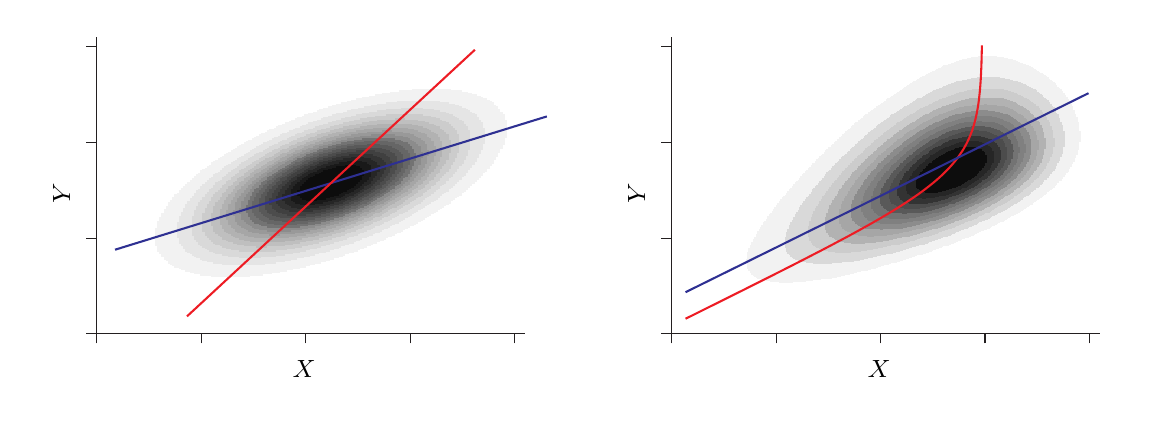
\begin{tikzpicture}[x=0.039cm,y=-0.039cm]
\useasboundingbox (0,0) rectangle (359,121);
\fill[chfourfig2c0] (125.1178,20.0029) rectangle (137.7724,20.4369);
\fill[chfourfig2c0] (120.8996,20.4369) rectangle (141.2876,20.8710);
\fill[chfourfig2c0] (118.0875,20.8710) rectangle (143.3967,21.3050);
\fill[chfourfig2c0] (115.2753,21.3050) rectangle (144.8028,21.7390);
\fill[chfourfig2c0] (113.1662,21.7390) rectangle (146.2088,22.1730);
\fill[chfourfig2c0] (111.0571,22.1730) rectangle (147.6149,22.6071);
\fill[chfourfig2c0] (108.9480,22.6071) rectangle (148.3180,23.0411);
\fill[chfourfig2c0] (106.8389,23.0411) rectangle (149.7240,23.4751);
\fill[chfourfig2c0] (105.4328,23.4751) rectangle (150.4271,23.9092);
\fill[chfourfig2c0] (104.0268,23.9092) rectangle (120.1966,24.3432);
\fill[chfourfig2c1] (120.1966,23.9092) rectangle (134.2573,24.3432);
\fill[chfourfig2c0] (134.2573,23.9092) rectangle (151.1301,24.3432);
\fill[chfourfig2c0] (101.9177,24.3432) rectangle (116.6814,24.7772);
\fill[chfourfig2c1] (116.6814,24.3432) rectangle (137.0694,24.7772);
\fill[chfourfig2c0] (137.0694,24.3432) rectangle (151.8331,24.7772);
\fill[chfourfig2c0] (100.5116,24.7772) rectangle (113.8692,25.2112);
\fill[chfourfig2c1] (113.8692,24.7772) rectangle (139.1785,25.2112);
\fill[chfourfig2c0] (139.1785,24.7772) rectangle (151.8331,25.2112);
\fill[chfourfig2c0] (99.1055,25.2112) rectangle (111.7601,25.6453);
\fill[chfourfig2c1] (111.7601,25.2112) rectangle (140.5846,25.6453);
\fill[chfourfig2c0] (140.5846,25.2112) rectangle (152.5362,25.6453);
\fill[chfourfig2c0] (97.6994,25.6453) rectangle (109.6510,26.0793);
\fill[chfourfig2c1] (109.6510,25.6453) rectangle (141.2876,26.0793);
\fill[chfourfig2c0] (141.2876,25.6453) rectangle (153.2392,26.0793);
\fill[chfourfig2c0] (96.2934,26.0793) rectangle (107.5419,26.5133);
\fill[chfourfig2c1] (107.5419,26.0793) rectangle (121.6026,26.5133);
\fill[chfourfig2c2] (121.6026,26.0793) rectangle (128.6330,26.5133);
\fill[chfourfig2c1] (128.6330,26.0793) rectangle (142.6937,26.5133);
\fill[chfourfig2c0] (142.6937,26.0793) rectangle (153.2392,26.5133);
\fill[chfourfig2c0] (94.8873,26.5133) rectangle (105.4328,26.9474);
\fill[chfourfig2c1] (105.4328,26.5133) rectangle (116.6814,26.9474);
\fill[chfourfig2c2] (116.6814,26.5133) rectangle (132.1482,26.9474);
\fill[chfourfig2c1] (132.1482,26.5133) rectangle (143.3967,26.9474);
\fill[chfourfig2c0] (143.3967,26.5133) rectangle (153.9422,26.9474);
\fill[chfourfig2c0] (94.1843,26.9474) rectangle (104.0268,27.3814);
\fill[chfourfig2c1] (104.0268,26.9474) rectangle (113.8692,27.3814);
\fill[chfourfig2c2] (113.8692,26.9474) rectangle (134.2573,27.3814);
\fill[chfourfig2c1] (134.2573,26.9474) rectangle (144.0997,27.3814);
\fill[chfourfig2c0] (144.0997,26.9474) rectangle (153.9422,27.3814);
\fill[chfourfig2c0] (92.7782,27.3814) rectangle (102.6207,27.8154);
\fill[chfourfig2c1] (102.6207,27.3814) rectangle (111.0571,27.8154);
\fill[chfourfig2c2] (111.0571,27.3814) rectangle (136.3664,27.8154);
\fill[chfourfig2c1] (136.3664,27.3814) rectangle (144.8028,27.8154);
\fill[chfourfig2c0] (144.8028,27.3814) rectangle (154.6453,27.8154);
\fill[chfourfig2c0] (91.3721,27.8154) rectangle (100.5116,28.2495);
\fill[chfourfig2c1] (100.5116,27.8154) rectangle (108.9480,28.2495);
\fill[chfourfig2c2] (108.9480,27.8154) rectangle (137.0694,28.2495);
\fill[chfourfig2c1] (137.0694,27.8154) rectangle (145.5058,28.2495);
\fill[chfourfig2c0] (145.5058,27.8154) rectangle (154.6453,28.2495);
\fill[chfourfig2c0] (89.9661,28.2495) rectangle (99.1055,28.6835);
\fill[chfourfig2c1] (99.1055,28.2495) rectangle (106.8389,28.6835);
\fill[chfourfig2c2] (106.8389,28.2495) rectangle (116.6814,28.6835);
\fill[chfourfig2c3] (116.6814,28.2495) rectangle (128.6330,28.6835);
\fill[chfourfig2c2] (128.6330,28.2495) rectangle (138.4755,28.6835);
\fill[chfourfig2c1] (138.4755,28.2495) rectangle (146.2088,28.6835);
\fill[chfourfig2c0] (146.2088,28.2495) rectangle (155.3483,29.1175);
\fill[chfourfig2c0] (89.2630,28.6835) rectangle (97.6994,29.1175);
\fill[chfourfig2c1] (97.6994,28.6835) rectangle (105.4328,29.1175);
\fill[chfourfig2c2] (105.4328,28.6835) rectangle (113.1662,29.1175);
\fill[chfourfig2c3] (113.1662,28.6835) rectangle (131.4451,29.1175);
\fill[chfourfig2c2] (131.4451,28.6835) rectangle (139.1785,29.1175);
\fill[chfourfig2c1] (139.1785,28.6835) rectangle (146.2088,29.1175);
\fill[chfourfig2c0] (87.8570,29.1175) rectangle (96.2934,29.5515);
\fill[chfourfig2c1] (96.2934,29.1175) rectangle (103.3237,29.5515);
\fill[chfourfig2c2] (103.3237,29.1175) rectangle (110.3541,29.5515);
\fill[chfourfig2c3] (110.3541,29.1175) rectangle (132.8512,29.5515);
\fill[chfourfig2c2] (132.8512,29.1175) rectangle (139.8815,29.5515);
\fill[chfourfig2c1] (139.8815,29.1175) rectangle (146.9119,29.5515);
\fill[chfourfig2c0] (146.9119,29.1175) rectangle (155.3483,29.9856);
\fill[chfourfig2c0] (87.1539,29.5515) rectangle (95.5903,29.9856);
\fill[chfourfig2c1] (95.5903,29.5515) rectangle (101.9177,29.9856);
\fill[chfourfig2c2] (101.9177,29.5515) rectangle (108.2450,29.9856);
\fill[chfourfig2c3] (108.2450,29.5515) rectangle (119.4935,29.9856);
\fill[chfourfig2c4] (119.4935,29.5515) rectangle (123.0087,29.9856);
\fill[chfourfig2c3] (123.0087,29.5515) rectangle (134.2573,29.9856);
\fill[chfourfig2c2] (134.2573,29.5515) rectangle (140.5846,29.9856);
\fill[chfourfig2c1] (140.5846,29.5515) rectangle (146.9119,29.9856);
\fill[chfourfig2c0] (85.7479,29.9856) rectangle (94.1843,30.4196);
\fill[chfourfig2c1] (94.1843,29.9856) rectangle (100.5116,30.4196);
\fill[chfourfig2c2] (100.5116,29.9856) rectangle (106.1359,30.4196);
\fill[chfourfig2c3] (106.1359,29.9856) rectangle (113.8692,30.4196);
\fill[chfourfig2c4] (113.8692,29.9856) rectangle (127.2269,30.4196);
\fill[chfourfig2c3] (127.2269,29.9856) rectangle (134.9603,30.4196);
\fill[chfourfig2c2] (134.9603,29.9856) rectangle (141.2876,30.4196);
\fill[chfourfig2c1] (141.2876,29.9856) rectangle (147.6149,30.4196);
\fill[chfourfig2c0] (147.6149,29.9856) rectangle (156.0513,30.8536);
\fill[chfourfig2c0] (85.0448,30.4196) rectangle (92.7782,30.8536);
\fill[chfourfig2c1] (92.7782,30.4196) rectangle (99.1055,30.8536);
\fill[chfourfig2c2] (99.1055,30.4196) rectangle (104.7298,30.8536);
\fill[chfourfig2c3] (104.7298,30.4196) rectangle (111.0571,30.8536);
\fill[chfourfig2c4] (111.0571,30.4196) rectangle (129.3360,30.8536);
\fill[chfourfig2c3] (129.3360,30.4196) rectangle (136.3664,30.8536);
\fill[chfourfig2c2] (136.3664,30.4196) rectangle (141.9906,30.8536);
\fill[chfourfig2c1] (141.9906,30.4196) rectangle (147.6149,30.8536);
\fill[chfourfig2c0] (83.6387,30.8536) rectangle (91.3721,31.2877);
\fill[chfourfig2c1] (91.3721,30.8536) rectangle (97.6994,31.2877);
\fill[chfourfig2c2] (97.6994,30.8536) rectangle (102.6207,31.2877);
\fill[chfourfig2c3] (102.6207,30.8536) rectangle (108.9480,31.2877);
\fill[chfourfig2c4] (108.9480,30.8536) rectangle (130.7421,31.2877);
\fill[chfourfig2c3] (130.7421,30.8536) rectangle (137.0694,31.2877);
\fill[chfourfig2c2] (137.0694,30.8536) rectangle (141.9906,31.2877);
\fill[chfourfig2c1] (141.9906,30.8536) rectangle (148.3180,31.2877);
\fill[chfourfig2c0] (82.9357,31.2877) rectangle (90.6691,31.7217);
\fill[chfourfig2c1] (90.6691,31.2877) rectangle (96.2934,31.7217);
\fill[chfourfig2c2] (96.2934,31.2877) rectangle (101.2146,31.7217);
\fill[chfourfig2c3] (101.2146,31.2877) rectangle (106.8389,31.7217);
\fill[chfourfig2c4] (106.8389,31.2877) rectangle (113.8692,31.7217);
\fill[chfourfig2c5] (113.8692,31.2877) rectangle (125.1178,31.7217);
\fill[chfourfig2c4] (125.1178,31.2877) rectangle (132.1482,31.7217);
\fill[chfourfig2c3] (132.1482,31.2877) rectangle (137.7724,31.7217);
\fill[chfourfig2c2] (137.7724,31.2877) rectangle (142.6937,32.1557);
\fill[chfourfig2c1] (142.6937,31.2877) rectangle (148.3180,32.1557);
\fill[chfourfig2c0] (81.5296,31.7217) rectangle (89.2630,32.1557);
\fill[chfourfig2c1] (89.2630,31.7217) rectangle (94.8873,32.1557);
\fill[chfourfig2c2] (94.8873,31.7217) rectangle (99.8086,32.1557);
\fill[chfourfig2c3] (99.8086,31.7217) rectangle (104.7298,32.1557);
\fill[chfourfig2c4] (104.7298,31.7217) rectangle (110.3541,32.1557);
\fill[chfourfig2c5] (110.3541,31.7217) rectangle (127.2269,32.1557);
\fill[chfourfig2c4] (127.2269,31.7217) rectangle (132.8512,32.1557);
\fill[chfourfig2c3] (132.8512,31.7217) rectangle (137.7724,32.1557);
\fill[chfourfig2c0] (148.3180,30.8536) rectangle (156.0513,32.5898);
\fill[chfourfig2c0] (80.8266,32.1557) rectangle (88.5600,32.5898);
\fill[chfourfig2c1] (88.5600,32.1557) rectangle (93.4812,32.5898);
\fill[chfourfig2c2] (93.4812,32.1557) rectangle (98.4025,32.5898);
\fill[chfourfig2c3] (98.4025,32.1557) rectangle (102.6207,32.5898);
\fill[chfourfig2c4] (102.6207,32.1557) rectangle (108.2450,32.5898);
\fill[chfourfig2c5] (108.2450,32.1557) rectangle (128.6330,32.5898);
\fill[chfourfig2c4] (128.6330,32.1557) rectangle (134.2573,32.5898);
\fill[chfourfig2c3] (134.2573,32.1557) rectangle (138.4755,32.5898);
\fill[chfourfig2c2] (138.4755,32.1557) rectangle (143.3967,32.5898);
\fill[chfourfig2c1] (143.3967,32.1557) rectangle (148.3180,32.5898);
\fill[chfourfig2c0] (80.1236,32.5898) rectangle (87.1539,33.0238);
\fill[chfourfig2c1] (87.1539,32.5898) rectangle (92.7782,33.0238);
\fill[chfourfig2c2] (92.7782,32.5898) rectangle (96.9964,33.0238);
\fill[chfourfig2c3] (96.9964,32.5898) rectangle (101.2146,33.0238);
\fill[chfourfig2c4] (101.2146,32.5898) rectangle (106.1359,33.0238);
\fill[chfourfig2c5] (106.1359,32.5898) rectangle (112.4632,33.0238);
\fill[chfourfig2c6] (112.4632,32.5898) rectangle (123.7117,33.0238);
\fill[chfourfig2c5] (123.7117,32.5898) rectangle (130.0390,33.0238);
\fill[chfourfig2c4] (130.0390,32.5898) rectangle (134.2573,33.0238);
\fill[chfourfig2c3] (134.2573,32.5898) rectangle (139.1785,33.0238);
\fill[chfourfig2c2] (139.1785,32.5898) rectangle (143.3967,33.4578);
\fill[chfourfig2c1] (143.3967,32.5898) rectangle (149.0210,33.4578);
\fill[chfourfig2c0] (78.7175,33.0238) rectangle (86.4509,33.4578);
\fill[chfourfig2c1] (86.4509,33.0238) rectangle (91.3721,33.4578);
\fill[chfourfig2c2] (91.3721,33.0238) rectangle (95.5903,33.4578);
\fill[chfourfig2c3] (95.5903,33.0238) rectangle (99.8086,33.4578);
\fill[chfourfig2c4] (99.8086,33.0238) rectangle (104.0268,33.4578);
\fill[chfourfig2c5] (104.0268,33.0238) rectangle (109.6510,33.4578);
\fill[chfourfig2c6] (109.6510,33.0238) rectangle (125.8208,33.4578);
\fill[chfourfig2c5] (125.8208,33.0238) rectangle (130.7421,33.4578);
\fill[chfourfig2c4] (130.7421,33.0238) rectangle (134.9603,33.4578);
\fill[chfourfig2c3] (134.9603,33.0238) rectangle (139.1785,33.4578);
\fill[chfourfig2c0] (78.0145,33.4578) rectangle (85.0448,33.8918);
\fill[chfourfig2c1] (85.0448,33.4578) rectangle (89.9661,33.8918);
\fill[chfourfig2c2] (89.9661,33.4578) rectangle (94.1843,33.8918);
\fill[chfourfig2c3] (94.1843,33.4578) rectangle (98.4025,33.8918);
\fill[chfourfig2c4] (98.4025,33.4578) rectangle (102.6207,33.8918);
\fill[chfourfig2c5] (102.6207,33.4578) rectangle (106.8389,33.8918);
\fill[chfourfig2c6] (106.8389,33.4578) rectangle (115.2753,33.8918);
\fill[chfourfig2c7] (115.2753,33.4578) rectangle (118.7905,33.8918);
\fill[chfourfig2c6] (118.7905,33.4578) rectangle (127.2269,33.8918);
\fill[chfourfig2c5] (127.2269,33.4578) rectangle (131.4451,33.8918);
\fill[chfourfig2c4] (131.4451,33.4578) rectangle (135.6633,33.8918);
\fill[chfourfig2c3] (135.6633,33.4578) rectangle (139.8815,33.8918);
\fill[chfourfig2c0] (77.3114,33.8918) rectangle (84.3418,34.3259);
\fill[chfourfig2c1] (84.3418,33.8918) rectangle (89.2630,34.3259);
\fill[chfourfig2c2] (89.2630,33.8918) rectangle (93.4812,34.3259);
\fill[chfourfig2c3] (93.4812,33.8918) rectangle (96.9964,34.3259);
\fill[chfourfig2c4] (96.9964,33.8918) rectangle (100.5116,34.3259);
\fill[chfourfig2c5] (100.5116,33.8918) rectangle (104.7298,34.3259);
\fill[chfourfig2c6] (104.7298,33.8918) rectangle (110.3541,34.3259);
\fill[chfourfig2c7] (110.3541,33.8918) rectangle (122.3057,34.3259);
\fill[chfourfig2c6] (122.3057,33.8918) rectangle (127.9299,34.3259);
\fill[chfourfig2c5] (127.9299,33.8918) rectangle (132.1482,34.3259);
\fill[chfourfig2c4] (132.1482,33.8918) rectangle (136.3664,34.3259);
\fill[chfourfig2c2] (139.8815,33.4578) rectangle (144.0997,34.7599);
\fill[chfourfig2c3] (136.3664,33.8918) rectangle (139.8815,34.7599);
\fill[chfourfig2c0] (75.9054,34.3259) rectangle (82.9357,34.7599);
\fill[chfourfig2c1] (82.9357,34.3259) rectangle (87.8570,34.7599);
\fill[chfourfig2c2] (87.8570,34.3259) rectangle (92.0752,34.7599);
\fill[chfourfig2c3] (92.0752,34.3259) rectangle (95.5903,34.7599);
\fill[chfourfig2c4] (95.5903,34.3259) rectangle (99.1055,34.7599);
\fill[chfourfig2c5] (99.1055,34.3259) rectangle (103.3237,34.7599);
\fill[chfourfig2c6] (103.3237,34.3259) rectangle (107.5419,34.7599);
\fill[chfourfig2c7] (107.5419,34.3259) rectangle (124.4148,34.7599);
\fill[chfourfig2c6] (124.4148,34.3259) rectangle (129.3360,34.7599);
\fill[chfourfig2c5] (129.3360,34.3259) rectangle (132.8512,34.7599);
\fill[chfourfig2c4] (132.8512,34.3259) rectangle (136.3664,34.7599);
\fill[chfourfig2c0] (75.2023,34.7599) rectangle (82.2327,35.1939);
\fill[chfourfig2c1] (82.2327,34.7599) rectangle (87.1539,35.1939);
\fill[chfourfig2c2] (87.1539,34.7599) rectangle (90.6691,35.1939);
\fill[chfourfig2c3] (90.6691,34.7599) rectangle (94.1843,35.1939);
\fill[chfourfig2c4] (94.1843,34.7599) rectangle (97.6994,35.1939);
\fill[chfourfig2c5] (97.6994,34.7599) rectangle (101.2146,35.1939);
\fill[chfourfig2c6] (101.2146,34.7599) rectangle (105.4328,35.1939);
\fill[chfourfig2c7] (105.4328,34.7599) rectangle (111.7601,35.1939);
\fill[chfourfig2c8] (111.7601,34.7599) rectangle (119.4935,35.1939);
\fill[chfourfig2c7] (119.4935,34.7599) rectangle (125.8208,35.1939);
\fill[chfourfig2c6] (125.8208,34.7599) rectangle (130.0390,35.1939);
\fill[chfourfig2c5] (130.0390,34.7599) rectangle (133.5542,35.6280);
\fill[chfourfig2c4] (133.5542,34.7599) rectangle (137.0694,35.6280);
\fill[chfourfig2c0] (74.4993,35.1939) rectangle (81.5296,35.6280);
\fill[chfourfig2c1] (81.5296,35.1939) rectangle (85.7479,35.6280);
\fill[chfourfig2c2] (85.7479,35.1939) rectangle (89.9661,35.6280);
\fill[chfourfig2c3] (89.9661,35.1939) rectangle (93.4812,35.6280);
\fill[chfourfig2c4] (93.4812,35.1939) rectangle (96.2934,35.6280);
\fill[chfourfig2c5] (96.2934,35.1939) rectangle (99.8086,35.6280);
\fill[chfourfig2c6] (99.8086,35.1939) rectangle (103.3237,35.6280);
\fill[chfourfig2c7] (103.3237,35.1939) rectangle (108.2450,35.6280);
\fill[chfourfig2c8] (108.2450,35.1939) rectangle (122.3057,35.6280);
\fill[chfourfig2c7] (122.3057,35.1939) rectangle (126.5239,35.6280);
\fill[chfourfig2c6] (126.5239,35.1939) rectangle (130.0390,35.6280);
\fill[chfourfig2c0] (149.0210,32.5898) rectangle (156.0513,36.0620);
\fill[chfourfig2c0] (73.7963,35.6280) rectangle (80.1236,36.0620);
\fill[chfourfig2c1] (80.1236,35.6280) rectangle (85.0448,36.0620);
\fill[chfourfig2c2] (85.0448,35.6280) rectangle (88.5600,36.0620);
\fill[chfourfig2c3] (88.5600,35.6280) rectangle (92.0752,36.0620);
\fill[chfourfig2c4] (92.0752,35.6280) rectangle (95.5903,36.0620);
\fill[chfourfig2c5] (95.5903,35.6280) rectangle (98.4025,36.0620);
\fill[chfourfig2c6] (98.4025,35.6280) rectangle (101.9177,36.0620);
\fill[chfourfig2c7] (101.9177,35.6280) rectangle (106.1359,36.0620);
\fill[chfourfig2c8] (106.1359,35.6280) rectangle (123.7117,36.0620);
\fill[chfourfig2c7] (123.7117,35.6280) rectangle (127.2269,36.0620);
\fill[chfourfig2c6] (127.2269,35.6280) rectangle (130.7421,36.0620);
\fill[chfourfig2c5] (130.7421,35.6280) rectangle (134.2573,36.0620);
\fill[chfourfig2c3] (137.0694,34.7599) rectangle (140.5846,36.4960);
\fill[chfourfig2c4] (134.2573,35.6280) rectangle (137.0694,36.4960);
\fill[chfourfig2c0] (73.0932,36.0620) rectangle (79.4205,36.4960);
\fill[chfourfig2c1] (79.4205,36.0620) rectangle (84.3418,36.4960);
\fill[chfourfig2c2] (84.3418,36.0620) rectangle (87.8570,36.4960);
\fill[chfourfig2c3] (87.8570,36.0620) rectangle (91.3721,36.4960);
\fill[chfourfig2c4] (91.3721,36.0620) rectangle (94.1843,36.4960);
\fill[chfourfig2c5] (94.1843,36.0620) rectangle (96.9964,36.4960);
\fill[chfourfig2c6] (96.9964,36.0620) rectangle (100.5116,36.4960);
\fill[chfourfig2c7] (100.5116,36.0620) rectangle (104.0268,36.4960);
\fill[chfourfig2c8] (104.0268,36.0620) rectangle (108.9480,36.4960);
\fill[chfourfig2c9] (108.9480,36.0620) rectangle (119.4935,36.4960);
\fill[chfourfig2c8] (119.4935,36.0620) rectangle (124.4148,36.4960);
\fill[chfourfig2c7] (124.4148,36.0620) rectangle (127.9299,36.4960);
\fill[chfourfig2c6] (127.9299,36.0620) rectangle (131.4451,36.4960);
\fill[chfourfig2c5] (131.4451,36.0620) rectangle (134.2573,36.9301);
\fill[chfourfig2c0] (71.6872,36.4960) rectangle (78.7175,36.9301);
\fill[chfourfig2c1] (78.7175,36.4960) rectangle (82.9357,36.9301);
\fill[chfourfig2c2] (82.9357,36.4960) rectangle (86.4509,36.9301);
\fill[chfourfig2c3] (86.4509,36.4960) rectangle (89.9661,36.9301);
\fill[chfourfig2c4] (89.9661,36.4960) rectangle (92.7782,36.9301);
\fill[chfourfig2c5] (92.7782,36.4960) rectangle (95.5903,36.9301);
\fill[chfourfig2c6] (95.5903,36.4960) rectangle (99.1055,36.9301);
\fill[chfourfig2c7] (99.1055,36.4960) rectangle (101.9177,36.9301);
\fill[chfourfig2c8] (101.9177,36.4960) rectangle (106.1359,36.9301);
\fill[chfourfig2c9] (106.1359,36.4960) rectangle (121.6026,36.9301);
\fill[chfourfig2c8] (121.6026,36.4960) rectangle (125.1178,36.9301);
\fill[chfourfig2c7] (125.1178,36.4960) rectangle (128.6330,36.9301);
\fill[chfourfig2c6] (128.6330,36.4960) rectangle (131.4451,36.9301);
\fill[chfourfig2c4] (134.2573,36.4960) rectangle (137.7724,36.9301);
\fill[chfourfig2c0] (70.9841,36.9301) rectangle (78.0145,37.3641);
\fill[chfourfig2c1] (78.0145,36.9301) rectangle (82.2327,37.3641);
\fill[chfourfig2c2] (82.2327,36.9301) rectangle (85.7479,37.3641);
\fill[chfourfig2c3] (85.7479,36.9301) rectangle (89.2630,37.3641);
\fill[chfourfig2c4] (89.2630,36.9301) rectangle (92.0752,37.3641);
\fill[chfourfig2c5] (92.0752,36.9301) rectangle (94.8873,37.3641);
\fill[chfourfig2c6] (94.8873,36.9301) rectangle (97.6994,37.3641);
\fill[chfourfig2c7] (97.6994,36.9301) rectangle (100.5116,37.3641);
\fill[chfourfig2c8] (100.5116,36.9301) rectangle (104.0268,37.3641);
\fill[chfourfig2c9] (104.0268,36.9301) rectangle (109.6510,37.3641);
\fill[chfourfig2c10] (109.6510,36.9301) rectangle (117.3844,37.3641);
\fill[chfourfig2c9] (117.3844,36.9301) rectangle (122.3057,37.3641);
\fill[chfourfig2c8] (122.3057,36.9301) rectangle (125.8208,37.3641);
\fill[chfourfig2c7] (125.8208,36.9301) rectangle (129.3360,37.3641);
\fill[chfourfig2c1] (144.0997,33.4578) rectangle (149.0210,37.7981);
\fill[chfourfig2c0] (149.0210,36.0620) rectangle (155.3483,37.7981);
\fill[chfourfig2c6] (129.3360,36.9301) rectangle (132.1482,37.7981);
\fill[chfourfig2c0] (70.2811,37.3641) rectangle (76.6084,37.7981);
\fill[chfourfig2c1] (76.6084,37.3641) rectangle (81.5296,37.7981);
\fill[chfourfig2c2] (81.5296,37.3641) rectangle (85.0448,37.7981);
\fill[chfourfig2c3] (85.0448,37.3641) rectangle (87.8570,37.7981);
\fill[chfourfig2c4] (87.8570,37.3641) rectangle (90.6691,37.7981);
\fill[chfourfig2c5] (90.6691,37.3641) rectangle (93.4812,37.7981);
\fill[chfourfig2c6] (93.4812,37.3641) rectangle (96.2934,37.7981);
\fill[chfourfig2c7] (96.2934,37.3641) rectangle (99.1055,37.7981);
\fill[chfourfig2c8] (99.1055,37.3641) rectangle (101.9177,37.7981);
\fill[chfourfig2c9] (101.9177,37.3641) rectangle (106.1359,37.7981);
\fill[chfourfig2c10] (106.1359,37.3641) rectangle (119.4935,37.7981);
\fill[chfourfig2c9] (119.4935,37.3641) rectangle (123.7117,37.7981);
\fill[chfourfig2c8] (123.7117,37.3641) rectangle (126.5239,37.7981);
\fill[chfourfig2c7] (126.5239,37.3641) rectangle (129.3360,37.7981);
\fill[chfourfig2c0] (69.5781,37.7981) rectangle (75.9054,38.2321);
\fill[chfourfig2c1] (75.9054,37.7981) rectangle (80.1236,38.2321);
\fill[chfourfig2c2] (80.1236,37.7981) rectangle (83.6387,38.2321);
\fill[chfourfig2c3] (83.6387,37.7981) rectangle (87.1539,38.2321);
\fill[chfourfig2c4] (87.1539,37.7981) rectangle (89.9661,38.2321);
\fill[chfourfig2c5] (89.9661,37.7981) rectangle (92.0752,38.2321);
\fill[chfourfig2c6] (92.0752,37.7981) rectangle (94.8873,38.2321);
\fill[chfourfig2c7] (94.8873,37.7981) rectangle (97.6994,38.2321);
\fill[chfourfig2c8] (97.6994,37.7981) rectangle (100.5116,38.2321);
\fill[chfourfig2c9] (100.5116,37.7981) rectangle (104.0268,38.2321);
\fill[chfourfig2c10] (104.0268,37.7981) rectangle (110.3541,38.2321);
\fill[chfourfig2c11] (110.3541,37.7981) rectangle (114.5723,38.2321);
\fill[chfourfig2c10] (114.5723,37.7981) rectangle (120.8996,38.2321);
\fill[chfourfig2c9] (120.8996,37.7981) rectangle (124.4148,38.2321);
\fill[chfourfig2c0] (148.3180,37.7981) rectangle (155.3483,38.2321);
\fill[chfourfig2c5] (132.1482,36.9301) rectangle (134.9603,38.6662);
\fill[chfourfig2c8] (124.4148,37.7981) rectangle (127.2269,38.6662);
\fill[chfourfig2c7] (127.2269,37.7981) rectangle (130.0390,38.6662);
\fill[chfourfig2c6] (130.0390,37.7981) rectangle (132.1482,38.6662);
\fill[chfourfig2c0] (68.8750,38.2321) rectangle (75.2023,38.6662);
\fill[chfourfig2c1] (75.2023,38.2321) rectangle (79.4205,38.6662);
\fill[chfourfig2c2] (79.4205,38.2321) rectangle (82.9357,38.6662);
\fill[chfourfig2c3] (82.9357,38.2321) rectangle (85.7479,38.6662);
\fill[chfourfig2c4] (85.7479,38.2321) rectangle (88.5600,38.6662);
\fill[chfourfig2c5] (88.5600,38.2321) rectangle (91.3721,38.6662);
\fill[chfourfig2c6] (91.3721,38.2321) rectangle (93.4812,38.6662);
\fill[chfourfig2c7] (93.4812,38.2321) rectangle (96.2934,38.6662);
\fill[chfourfig2c8] (96.2934,38.2321) rectangle (99.1055,38.6662);
\fill[chfourfig2c9] (99.1055,38.2321) rectangle (101.9177,38.6662);
\fill[chfourfig2c10] (101.9177,38.2321) rectangle (106.1359,38.6662);
\fill[chfourfig2c11] (106.1359,38.2321) rectangle (117.3844,38.6662);
\fill[chfourfig2c10] (117.3844,38.2321) rectangle (121.6026,38.6662);
\fill[chfourfig2c9] (121.6026,38.2321) rectangle (124.4148,38.6662);
\fill[chfourfig2c0] (68.1720,38.6662) rectangle (74.4993,39.1002);
\fill[chfourfig2c1] (74.4993,38.6662) rectangle (78.7175,39.1002);
\fill[chfourfig2c2] (78.7175,38.6662) rectangle (82.2327,39.1002);
\fill[chfourfig2c3] (82.2327,38.6662) rectangle (85.0448,39.1002);
\fill[chfourfig2c4] (85.0448,38.6662) rectangle (87.8570,39.1002);
\fill[chfourfig2c5] (87.8570,38.6662) rectangle (89.9661,39.1002);
\fill[chfourfig2c6] (89.9661,38.6662) rectangle (92.7782,39.1002);
\fill[chfourfig2c7] (92.7782,38.6662) rectangle (94.8873,39.1002);
\fill[chfourfig2c8] (94.8873,38.6662) rectangle (97.6994,39.1002);
\fill[chfourfig2c9] (97.6994,38.6662) rectangle (100.5116,39.1002);
\fill[chfourfig2c10] (100.5116,38.6662) rectangle (104.0268,39.1002);
\fill[chfourfig2c11] (104.0268,38.6662) rectangle (118.7905,39.1002);
\fill[chfourfig2c10] (118.7905,38.6662) rectangle (122.3057,39.1002);
\fill[chfourfig2c9] (122.3057,38.6662) rectangle (125.1178,39.1002);
\fill[chfourfig2c0] (148.3180,38.2321) rectangle (154.6453,39.5342);
\fill[chfourfig2c8] (125.1178,38.6662) rectangle (127.9299,39.5342);
\fill[chfourfig2c0] (67.4689,39.1002) rectangle (73.7963,39.5342);
\fill[chfourfig2c1] (73.7963,39.1002) rectangle (78.0145,39.5342);
\fill[chfourfig2c2] (78.0145,39.1002) rectangle (81.5296,39.5342);
\fill[chfourfig2c3] (81.5296,39.1002) rectangle (84.3418,39.5342);
\fill[chfourfig2c4] (84.3418,39.1002) rectangle (86.4509,39.5342);
\fill[chfourfig2c5] (86.4509,39.1002) rectangle (89.2630,39.5342);
\fill[chfourfig2c6] (89.2630,39.1002) rectangle (91.3721,39.5342);
\fill[chfourfig2c7] (91.3721,39.1002) rectangle (94.1843,39.5342);
\fill[chfourfig2c8] (94.1843,39.1002) rectangle (96.2934,39.5342);
\fill[chfourfig2c9] (96.2934,39.1002) rectangle (99.1055,39.5342);
\fill[chfourfig2c10] (99.1055,39.1002) rectangle (101.9177,39.5342);
\fill[chfourfig2c11] (101.9177,39.1002) rectangle (106.8389,39.5342);
\fill[chfourfig2c12] (106.8389,39.1002) rectangle (115.2753,39.5342);
\fill[chfourfig2c11] (115.2753,39.1002) rectangle (119.4935,39.5342);
\fill[chfourfig2c10] (119.4935,39.1002) rectangle (123.0087,39.5342);
\fill[chfourfig2c9] (123.0087,39.1002) rectangle (125.1178,39.5342);
\fill[chfourfig2c2] (140.5846,34.7599) rectangle (144.0997,39.9683);
\fill[chfourfig2c1] (144.0997,37.7981) rectangle (148.3180,39.9683);
\fill[chfourfig2c7] (127.9299,38.6662) rectangle (130.0390,39.9683);
\fill[chfourfig2c6] (130.0390,38.6662) rectangle (132.8512,39.9683);
\fill[chfourfig2c0] (66.7659,39.5342) rectangle (73.0932,39.9683);
\fill[chfourfig2c1] (73.0932,39.5342) rectangle (77.3114,39.9683);
\fill[chfourfig2c2] (77.3114,39.5342) rectangle (80.1236,39.9683);
\fill[chfourfig2c3] (80.1236,39.5342) rectangle (82.9357,39.9683);
\fill[chfourfig2c4] (82.9357,39.5342) rectangle (85.7479,39.9683);
\fill[chfourfig2c5] (85.7479,39.5342) rectangle (88.5600,39.9683);
\fill[chfourfig2c6] (88.5600,39.5342) rectangle (90.6691,39.9683);
\fill[chfourfig2c7] (90.6691,39.5342) rectangle (92.7782,39.9683);
\fill[chfourfig2c8] (92.7782,39.5342) rectangle (94.8873,39.9683);
\fill[chfourfig2c9] (94.8873,39.5342) rectangle (97.6994,39.9683);
\fill[chfourfig2c10] (97.6994,39.5342) rectangle (100.5116,39.9683);
\fill[chfourfig2c11] (100.5116,39.5342) rectangle (104.0268,39.9683);
\fill[chfourfig2c12] (104.0268,39.5342) rectangle (116.6814,39.9683);
\fill[chfourfig2c11] (116.6814,39.5342) rectangle (120.1966,39.9683);
\fill[chfourfig2c10] (120.1966,39.5342) rectangle (123.0087,39.9683);
\fill[chfourfig2c9] (123.0087,39.5342) rectangle (125.8208,39.9683);
\fill[chfourfig2c0] (148.3180,39.5342) rectangle (153.9422,39.9683);
\fill[chfourfig2c8] (125.8208,39.5342) rectangle (127.9299,40.4023);
\fill[chfourfig2c0] (66.0629,39.9683) rectangle (72.3902,40.4023);
\fill[chfourfig2c1] (72.3902,39.9683) rectangle (76.6084,40.4023);
\fill[chfourfig2c2] (76.6084,39.9683) rectangle (79.4205,40.4023);
\fill[chfourfig2c3] (79.4205,39.9683) rectangle (82.2327,40.4023);
\fill[chfourfig2c4] (82.2327,39.9683) rectangle (85.0448,40.4023);
\fill[chfourfig2c5] (85.0448,39.9683) rectangle (87.1539,40.4023);
\fill[chfourfig2c6] (87.1539,39.9683) rectangle (89.2630,40.4023);
\fill[chfourfig2c7] (89.2630,39.9683) rectangle (92.0752,40.4023);
\fill[chfourfig2c8] (92.0752,39.9683) rectangle (94.1843,40.4023);
\fill[chfourfig2c9] (94.1843,39.9683) rectangle (96.2934,40.4023);
\fill[chfourfig2c10] (96.2934,39.9683) rectangle (99.1055,40.4023);
\fill[chfourfig2c11] (99.1055,39.9683) rectangle (101.9177,40.4023);
\fill[chfourfig2c12] (101.9177,39.9683) rectangle (106.8389,40.4023);
\fill[chfourfig2c13] (106.8389,39.9683) rectangle (113.1662,40.4023);
\fill[chfourfig2c12] (113.1662,39.9683) rectangle (118.0875,40.4023);
\fill[chfourfig2c11] (118.0875,39.9683) rectangle (120.8996,40.4023);
\fill[chfourfig2c10] (120.8996,39.9683) rectangle (123.7117,40.4023);
\fill[chfourfig2c7] (127.9299,39.9683) rectangle (130.7421,40.4023);
\fill[chfourfig2c3] (137.7724,36.4960) rectangle (140.5846,40.8363);
\fill[chfourfig2c4] (134.9603,36.9301) rectangle (137.7724,40.8363);
\fill[chfourfig2c9] (123.7117,39.9683) rectangle (125.8208,40.8363);
\fill[chfourfig2c2] (140.5846,39.9683) rectangle (143.3967,40.8363);
\fill[chfourfig2c0] (147.6149,39.9683) rectangle (153.9422,40.8363);
\fill[chfourfig2c0] (65.3598,40.4023) rectangle (71.6872,40.8363);
\fill[chfourfig2c1] (71.6872,40.4023) rectangle (75.2023,40.8363);
\fill[chfourfig2c2] (75.2023,40.4023) rectangle (78.7175,40.8363);
\fill[chfourfig2c3] (78.7175,40.4023) rectangle (81.5296,40.8363);
\fill[chfourfig2c4] (81.5296,40.4023) rectangle (84.3418,40.8363);
\fill[chfourfig2c5] (84.3418,40.4023) rectangle (86.4509,40.8363);
\fill[chfourfig2c6] (86.4509,40.4023) rectangle (88.5600,40.8363);
\fill[chfourfig2c7] (88.5600,40.4023) rectangle (90.6691,40.8363);
\fill[chfourfig2c8] (90.6691,40.4023) rectangle (92.7782,40.8363);
\fill[chfourfig2c9] (92.7782,40.4023) rectangle (94.8873,40.8363);
\fill[chfourfig2c10] (94.8873,40.4023) rectangle (97.6994,40.8363);
\fill[chfourfig2c11] (97.6994,40.4023) rectangle (100.5116,40.8363);
\fill[chfourfig2c12] (100.5116,40.4023) rectangle (104.0268,40.8363);
\fill[chfourfig2c13] (104.0268,40.4023) rectangle (114.5723,40.8363);
\fill[chfourfig2c12] (114.5723,40.4023) rectangle (118.7905,40.8363);
\fill[chfourfig2c11] (118.7905,40.4023) rectangle (121.6026,40.8363);
\fill[chfourfig2c10] (121.6026,40.4023) rectangle (123.7117,40.8363);
\fill[chfourfig2c8] (125.8208,40.4023) rectangle (128.6330,40.8363);
\fill[chfourfig2c1] (143.3967,39.9683) rectangle (147.6149,41.2704);
\fill[chfourfig2c0] (64.6568,40.8363) rectangle (70.9841,41.2704);
\fill[chfourfig2c1] (70.9841,40.8363) rectangle (74.4993,41.2704);
\fill[chfourfig2c2] (74.4993,40.8363) rectangle (78.0145,41.2704);
\fill[chfourfig2c3] (78.0145,40.8363) rectangle (80.8266,41.2704);
\fill[chfourfig2c4] (80.8266,40.8363) rectangle (82.9357,41.2704);
\fill[chfourfig2c5] (82.9357,40.8363) rectangle (85.7479,41.2704);
\fill[chfourfig2c6] (85.7479,40.8363) rectangle (87.8570,41.2704);
\fill[chfourfig2c7] (87.8570,40.8363) rectangle (89.9661,41.2704);
\fill[chfourfig2c8] (89.9661,40.8363) rectangle (92.0752,41.2704);
\fill[chfourfig2c9] (92.0752,40.8363) rectangle (94.1843,41.2704);
\fill[chfourfig2c10] (94.1843,40.8363) rectangle (96.2934,41.2704);
\fill[chfourfig2c11] (96.2934,40.8363) rectangle (99.1055,41.2704);
\fill[chfourfig2c12] (99.1055,40.8363) rectangle (101.9177,41.2704);
\fill[chfourfig2c13] (101.9177,40.8363) rectangle (115.9784,41.2704);
\fill[chfourfig2c12] (115.9784,40.8363) rectangle (119.4935,41.2704);
\fill[chfourfig2c11] (119.4935,40.8363) rectangle (121.6026,41.2704);
\fill[chfourfig2c10] (121.6026,40.8363) rectangle (124.4148,41.2704);
\fill[chfourfig2c0] (147.6149,40.8363) rectangle (153.2392,41.2704);
\fill[chfourfig2c5] (132.8512,38.6662) rectangle (134.9603,41.7044);
\fill[chfourfig2c6] (130.7421,39.9683) rectangle (132.8512,41.7044);
\fill[chfourfig2c7] (128.6330,40.4023) rectangle (130.7421,41.7044);
\fill[chfourfig2c2] (139.8815,40.8363) rectangle (143.3967,41.7044);
\fill[chfourfig2c0] (63.9538,41.2704) rectangle (70.2811,41.7044);
\fill[chfourfig2c1] (70.2811,41.2704) rectangle (73.7963,41.7044);
\fill[chfourfig2c2] (73.7963,41.2704) rectangle (77.3114,41.7044);
\fill[chfourfig2c3] (77.3114,41.2704) rectangle (80.1236,41.7044);
\fill[chfourfig2c4] (80.1236,41.2704) rectangle (82.2327,41.7044);
\fill[chfourfig2c5] (82.2327,41.2704) rectangle (84.3418,41.7044);
\fill[chfourfig2c6] (84.3418,41.2704) rectangle (86.4509,41.7044);
\fill[chfourfig2c7] (86.4509,41.2704) rectangle (88.5600,41.7044);
\fill[chfourfig2c8] (88.5600,41.2704) rectangle (90.6691,41.7044);
\fill[chfourfig2c9] (90.6691,41.2704) rectangle (92.7782,41.7044);
\fill[chfourfig2c10] (92.7782,41.2704) rectangle (94.8873,41.7044);
\fill[chfourfig2c11] (94.8873,41.2704) rectangle (97.6994,41.7044);
\fill[chfourfig2c12] (97.6994,41.2704) rectangle (100.5116,41.7044);
\fill[chfourfig2c13] (100.5116,41.2704) rectangle (104.7298,41.7044);
\fill[chfourfig2c14] (104.7298,41.2704) rectangle (112.4632,41.7044);
\fill[chfourfig2c13] (112.4632,41.2704) rectangle (116.6814,41.7044);
\fill[chfourfig2c12] (116.6814,41.2704) rectangle (119.4935,41.7044);
\fill[chfourfig2c11] (119.4935,41.2704) rectangle (122.3057,41.7044);
\fill[chfourfig2c1] (143.3967,41.2704) rectangle (146.9119,41.7044);
\fill[chfourfig2c4] (134.9603,40.8363) rectangle (137.0694,42.1384);
\fill[chfourfig2c0] (146.9119,41.2704) rectangle (153.2392,42.1384);
\fill[chfourfig2c0] (63.2507,41.7044) rectangle (69.5781,42.1384);
\fill[chfourfig2c1] (69.5781,41.7044) rectangle (73.0932,42.1384);
\fill[chfourfig2c2] (73.0932,41.7044) rectangle (76.6084,42.1384);
\fill[chfourfig2c3] (76.6084,41.7044) rectangle (79.4205,42.1384);
\fill[chfourfig2c4] (79.4205,41.7044) rectangle (81.5296,42.1384);
\fill[chfourfig2c5] (81.5296,41.7044) rectangle (83.6387,42.1384);
\fill[chfourfig2c6] (83.6387,41.7044) rectangle (85.7479,42.1384);
\fill[chfourfig2c7] (85.7479,41.7044) rectangle (87.8570,42.1384);
\fill[chfourfig2c8] (87.8570,41.7044) rectangle (89.9661,42.1384);
\fill[chfourfig2c9] (89.9661,41.7044) rectangle (92.0752,42.1384);
\fill[chfourfig2c10] (92.0752,41.7044) rectangle (94.1843,42.1384);
\fill[chfourfig2c11] (94.1843,41.7044) rectangle (96.2934,42.1384);
\fill[chfourfig2c12] (96.2934,41.7044) rectangle (99.1055,42.1384);
\fill[chfourfig2c13] (99.1055,41.7044) rectangle (101.9177,42.1384);
\fill[chfourfig2c14] (101.9177,41.7044) rectangle (113.8692,42.1384);
\fill[chfourfig2c13] (113.8692,41.7044) rectangle (117.3844,42.1384);
\fill[chfourfig2c12] (117.3844,41.7044) rectangle (120.1966,42.1384);
\fill[chfourfig2c5] (132.1482,41.7044) rectangle (134.9603,42.1384);
\fill[chfourfig2c8] (126.5239,40.8363) rectangle (128.6330,42.5724);
\fill[chfourfig2c3] (137.0694,40.8363) rectangle (139.8815,42.5724);
\fill[chfourfig2c7] (128.6330,41.7044) rectangle (130.0390,42.5724);
\fill[chfourfig2c2] (139.8815,41.7044) rectangle (142.6937,42.5724);
\fill[chfourfig2c1] (142.6937,41.7044) rectangle (146.9119,42.5724);
\fill[chfourfig2c0] (62.5477,42.1384) rectangle (68.8750,42.5724);
\fill[chfourfig2c1] (68.8750,42.1384) rectangle (72.3902,42.5724);
\fill[chfourfig2c2] (72.3902,42.1384) rectangle (75.9054,42.5724);
\fill[chfourfig2c3] (75.9054,42.1384) rectangle (78.7175,42.5724);
\fill[chfourfig2c4] (78.7175,42.1384) rectangle (80.8266,42.5724);
\fill[chfourfig2c5] (80.8266,42.1384) rectangle (82.9357,42.5724);
\fill[chfourfig2c6] (82.9357,42.1384) rectangle (85.0448,42.5724);
\fill[chfourfig2c7] (85.0448,42.1384) rectangle (87.1539,42.5724);
\fill[chfourfig2c8] (87.1539,42.1384) rectangle (89.2630,42.5724);
\fill[chfourfig2c9] (89.2630,42.1384) rectangle (90.6691,42.5724);
\fill[chfourfig2c10] (90.6691,42.1384) rectangle (92.7782,42.5724);
\fill[chfourfig2c11] (92.7782,42.1384) rectangle (94.8873,42.5724);
\fill[chfourfig2c12] (94.8873,42.1384) rectangle (97.6994,42.5724);
\fill[chfourfig2c13] (97.6994,42.1384) rectangle (100.5116,42.5724);
\fill[chfourfig2c14] (100.5116,42.1384) rectangle (105.4328,42.5724);
\fill[chfourfig2c15] (105.4328,42.1384) rectangle (109.6510,42.5724);
\fill[chfourfig2c14] (109.6510,42.1384) rectangle (114.5723,42.5724);
\fill[chfourfig2c13] (114.5723,42.1384) rectangle (118.0875,42.5724);
\fill[chfourfig2c0] (146.9119,42.1384) rectangle (152.5362,42.5724);
\fill[chfourfig2c4] (134.2573,42.1384) rectangle (137.0694,43.0065);
\fill[chfourfig2c0] (61.8447,42.5724) rectangle (68.1720,43.0065);
\fill[chfourfig2c1] (68.1720,42.5724) rectangle (71.6872,43.0065);
\fill[chfourfig2c2] (71.6872,42.5724) rectangle (75.2023,43.0065);
\fill[chfourfig2c3] (75.2023,42.5724) rectangle (77.3114,43.0065);
\fill[chfourfig2c4] (77.3114,42.5724) rectangle (80.1236,43.0065);
\fill[chfourfig2c5] (80.1236,42.5724) rectangle (82.2327,43.0065);
\fill[chfourfig2c6] (82.2327,42.5724) rectangle (84.3418,43.0065);
\fill[chfourfig2c7] (84.3418,42.5724) rectangle (86.4509,43.0065);
\fill[chfourfig2c8] (86.4509,42.5724) rectangle (87.8570,43.0065);
\fill[chfourfig2c9] (87.8570,42.5724) rectangle (89.9661,43.0065);
\fill[chfourfig2c10] (89.9661,42.5724) rectangle (92.0752,43.0065);
\fill[chfourfig2c11] (92.0752,42.5724) rectangle (94.1843,43.0065);
\fill[chfourfig2c12] (94.1843,42.5724) rectangle (96.2934,43.0065);
\fill[chfourfig2c13] (96.2934,42.5724) rectangle (99.1055,43.0065);
\fill[chfourfig2c14] (99.1055,42.5724) rectangle (102.6207,43.0065);
\fill[chfourfig2c15] (102.6207,42.5724) rectangle (111.7601,43.0065);
\fill[chfourfig2c14] (111.7601,42.5724) rectangle (115.2753,43.0065);
\fill[chfourfig2c13] (115.2753,42.5724) rectangle (118.0875,43.0065);
\fill[chfourfig2c3] (137.0694,42.5724) rectangle (139.1785,43.0065);
\fill[chfourfig2c2] (139.1785,42.5724) rectangle (142.6937,43.0065);
\fill[chfourfig2c1] (142.6937,42.5724) rectangle (146.2088,43.0065);
\fill[chfourfig2c0] (146.2088,42.5724) rectangle (152.5362,43.0065);
\fill[chfourfig2c9] (124.4148,40.8363) rectangle (126.5239,43.4405);
\fill[chfourfig2c12] (118.0875,42.1384) rectangle (120.1966,43.4405);
\fill[chfourfig2c8] (126.5239,42.5724) rectangle (127.9299,43.4405);
\fill[chfourfig2c0] (61.1416,43.0065) rectangle (67.4689,43.4405);
\fill[chfourfig2c1] (67.4689,43.0065) rectangle (70.9841,43.4405);
\fill[chfourfig2c2] (70.9841,43.0065) rectangle (74.4993,43.4405);
\fill[chfourfig2c3] (74.4993,43.0065) rectangle (76.6084,43.4405);
\fill[chfourfig2c4] (76.6084,43.0065) rectangle (79.4205,43.4405);
\fill[chfourfig2c5] (79.4205,43.0065) rectangle (81.5296,43.4405);
\fill[chfourfig2c6] (81.5296,43.0065) rectangle (83.6387,43.4405);
\fill[chfourfig2c7] (83.6387,43.0065) rectangle (85.0448,43.4405);
\fill[chfourfig2c8] (85.0448,43.0065) rectangle (87.1539,43.4405);
\fill[chfourfig2c9] (87.1539,43.0065) rectangle (89.2630,43.4405);
\fill[chfourfig2c10] (89.2630,43.0065) rectangle (90.6691,43.4405);
\fill[chfourfig2c11] (90.6691,43.0065) rectangle (92.7782,43.4405);
\fill[chfourfig2c12] (92.7782,43.0065) rectangle (94.8873,43.4405);
\fill[chfourfig2c13] (94.8873,43.0065) rectangle (97.6994,43.4405);
\fill[chfourfig2c14] (97.6994,43.0065) rectangle (100.5116,43.4405);
\fill[chfourfig2c15] (100.5116,43.0065) rectangle (112.4632,43.4405);
\fill[chfourfig2c14] (112.4632,43.0065) rectangle (115.9784,43.4405);
\fill[chfourfig2c13] (115.9784,43.0065) rectangle (118.0875,43.4405);
\fill[chfourfig2c6] (130.0390,41.7044) rectangle (132.1482,43.8745);
\fill[chfourfig2c5] (132.1482,42.1384) rectangle (134.2573,43.8745);
\fill[chfourfig2c4] (134.2573,43.0065) rectangle (136.3664,43.8745);
\fill[chfourfig2c3] (136.3664,43.0065) rectangle (139.1785,43.8745);
\fill[chfourfig2c2] (139.1785,43.0065) rectangle (141.9906,43.8745);
\fill[chfourfig2c1] (141.9906,43.0065) rectangle (146.2088,43.8745);
\fill[chfourfig2c0] (146.2088,43.0065) rectangle (151.8331,43.8745);
\fill[chfourfig2c0] (60.4386,43.4405) rectangle (66.7659,43.8745);
\fill[chfourfig2c1] (66.7659,43.4405) rectangle (70.2811,43.8745);
\fill[chfourfig2c2] (70.2811,43.4405) rectangle (73.7963,43.8745);
\fill[chfourfig2c3] (73.7963,43.4405) rectangle (75.9054,43.8745);
\fill[chfourfig2c4] (75.9054,43.4405) rectangle (78.7175,43.8745);
\fill[chfourfig2c5] (78.7175,43.4405) rectangle (80.8266,43.8745);
\fill[chfourfig2c6] (80.8266,43.4405) rectangle (82.9357,43.8745);
\fill[chfourfig2c7] (82.9357,43.4405) rectangle (84.3418,43.8745);
\fill[chfourfig2c8] (84.3418,43.4405) rectangle (86.4509,43.8745);
\fill[chfourfig2c9] (86.4509,43.4405) rectangle (88.5600,43.8745);
\fill[chfourfig2c10] (88.5600,43.4405) rectangle (89.9661,43.8745);
\fill[chfourfig2c11] (89.9661,43.4405) rectangle (92.0752,43.8745);
\fill[chfourfig2c12] (92.0752,43.4405) rectangle (94.1843,43.8745);
\fill[chfourfig2c13] (94.1843,43.4405) rectangle (96.2934,43.8745);
\fill[chfourfig2c14] (96.2934,43.4405) rectangle (99.1055,43.8745);
\fill[chfourfig2c15] (99.1055,43.4405) rectangle (104.0268,43.8745);
\fill[chfourfig2c16] (104.0268,43.4405) rectangle (108.9480,43.8745);
\fill[chfourfig2c15] (108.9480,43.4405) rectangle (113.1662,43.8745);
\fill[chfourfig2c14] (113.1662,43.4405) rectangle (115.9784,43.8745);
\fill[chfourfig2c13] (115.9784,43.4405) rectangle (118.7905,43.8745);
\fill[chfourfig2c7] (127.9299,42.5724) rectangle (130.0390,44.3086);
\fill[chfourfig2c0] (59.7356,43.8745) rectangle (66.0629,44.3086);
\fill[chfourfig2c1] (66.0629,43.8745) rectangle (69.5781,44.3086);
\fill[chfourfig2c2] (69.5781,43.8745) rectangle (73.0932,44.3086);
\fill[chfourfig2c3] (73.0932,43.8745) rectangle (75.2023,44.3086);
\fill[chfourfig2c4] (75.2023,43.8745) rectangle (78.0145,44.3086);
\fill[chfourfig2c5] (78.0145,43.8745) rectangle (80.1236,44.3086);
\fill[chfourfig2c6] (80.1236,43.8745) rectangle (81.5296,44.3086);
\fill[chfourfig2c7] (81.5296,43.8745) rectangle (83.6387,44.3086);
\fill[chfourfig2c8] (83.6387,43.8745) rectangle (85.7479,44.3086);
\fill[chfourfig2c9] (85.7479,43.8745) rectangle (87.1539,44.3086);
\fill[chfourfig2c10] (87.1539,43.8745) rectangle (89.2630,44.3086);
\fill[chfourfig2c11] (89.2630,43.8745) rectangle (91.3721,44.3086);
\fill[chfourfig2c12] (91.3721,43.8745) rectangle (92.7782,44.3086);
\fill[chfourfig2c13] (92.7782,43.8745) rectangle (94.8873,44.3086);
\fill[chfourfig2c14] (94.8873,43.8745) rectangle (97.6994,44.3086);
\fill[chfourfig2c15] (97.6994,43.8745) rectangle (101.2146,44.3086);
\fill[chfourfig2c16] (101.2146,43.8745) rectangle (110.3541,44.3086);
\fill[chfourfig2c15] (110.3541,43.8745) rectangle (113.8692,44.3086);
\fill[chfourfig2c6] (130.0390,43.8745) rectangle (131.4451,44.3086);
\fill[chfourfig2c4] (133.5542,43.8745) rectangle (136.3664,44.3086);
\fill[chfourfig2c3] (136.3664,43.8745) rectangle (138.4755,44.3086);
\fill[chfourfig2c2] (138.4755,43.8745) rectangle (141.9906,44.3086);
\fill[chfourfig2c1] (141.9906,43.8745) rectangle (145.5058,44.3086);
\fill[chfourfig2c0] (145.5058,43.8745) rectangle (151.8331,44.3086);
\fill[chfourfig2c10] (122.3057,41.2704) rectangle (124.4148,44.7426);
\fill[chfourfig2c9] (124.4148,43.4405) rectangle (125.8208,44.7426);
\fill[chfourfig2c8] (125.8208,43.4405) rectangle (127.9299,44.7426);
\fill[chfourfig2c14] (113.8692,43.8745) rectangle (116.6814,44.7426);
\fill[chfourfig2c0] (59.7356,44.3086) rectangle (65.3598,44.7426);
\fill[chfourfig2c1] (65.3598,44.3086) rectangle (68.8750,44.7426);
\fill[chfourfig2c2] (68.8750,44.3086) rectangle (72.3902,44.7426);
\fill[chfourfig2c3] (72.3902,44.3086) rectangle (74.4993,44.7426);
\fill[chfourfig2c4] (74.4993,44.3086) rectangle (77.3114,44.7426);
\fill[chfourfig2c5] (77.3114,44.3086) rectangle (79.4205,44.7426);
\fill[chfourfig2c6] (79.4205,44.3086) rectangle (80.8266,44.7426);
\fill[chfourfig2c7] (80.8266,44.3086) rectangle (82.9357,44.7426);
\fill[chfourfig2c8] (82.9357,44.3086) rectangle (85.0448,44.7426);
\fill[chfourfig2c9] (85.0448,44.3086) rectangle (86.4509,44.7426);
\fill[chfourfig2c10] (86.4509,44.3086) rectangle (88.5600,44.7426);
\fill[chfourfig2c11] (88.5600,44.3086) rectangle (89.9661,44.7426);
\fill[chfourfig2c12] (89.9661,44.3086) rectangle (92.0752,44.7426);
\fill[chfourfig2c13] (92.0752,44.3086) rectangle (94.1843,44.7426);
\fill[chfourfig2c14] (94.1843,44.3086) rectangle (96.2934,44.7426);
\fill[chfourfig2c15] (96.2934,44.3086) rectangle (99.8086,44.7426);
\fill[chfourfig2c16] (99.8086,44.3086) rectangle (111.0571,44.7426);
\fill[chfourfig2c15] (111.0571,44.3086) rectangle (113.8692,44.7426);
\fill[chfourfig2c7] (127.9299,44.3086) rectangle (129.3360,44.7426);
\fill[chfourfig2c3] (135.6633,44.3086) rectangle (138.4755,44.7426);
\fill[chfourfig2c2] (138.4755,44.3086) rectangle (141.2876,44.7426);
\fill[chfourfig2c1] (141.2876,44.3086) rectangle (145.5058,44.7426);
\fill[chfourfig2c0] (145.5058,44.3086) rectangle (151.1301,44.7426);
\fill[chfourfig2c5] (131.4451,43.8745) rectangle (133.5542,45.1766);
\fill[chfourfig2c6] (129.3360,44.3086) rectangle (131.4451,45.1766);
\fill[chfourfig2c4] (133.5542,44.3086) rectangle (135.6633,45.1766);
\fill[chfourfig2c0] (59.0325,44.7426) rectangle (64.6568,45.1766);
\fill[chfourfig2c1] (64.6568,44.7426) rectangle (68.8750,45.1766);
\fill[chfourfig2c2] (68.8750,44.7426) rectangle (71.6872,45.1766);
\fill[chfourfig2c3] (71.6872,44.7426) rectangle (74.4993,45.1766);
\fill[chfourfig2c4] (74.4993,44.7426) rectangle (76.6084,45.1766);
\fill[chfourfig2c5] (76.6084,44.7426) rectangle (78.7175,45.1766);
\fill[chfourfig2c6] (78.7175,44.7426) rectangle (80.1236,45.1766);
\fill[chfourfig2c7] (80.1236,44.7426) rectangle (82.2327,45.1766);
\fill[chfourfig2c8] (82.2327,44.7426) rectangle (84.3418,45.1766);
\fill[chfourfig2c9] (84.3418,44.7426) rectangle (85.7479,45.1766);
\fill[chfourfig2c10] (85.7479,44.7426) rectangle (87.8570,45.1766);
\fill[chfourfig2c11] (87.8570,44.7426) rectangle (89.2630,45.1766);
\fill[chfourfig2c12] (89.2630,44.7426) rectangle (91.3721,45.1766);
\fill[chfourfig2c13] (91.3721,44.7426) rectangle (93.4812,45.1766);
\fill[chfourfig2c14] (93.4812,44.7426) rectangle (95.5903,45.1766);
\fill[chfourfig2c15] (95.5903,44.7426) rectangle (98.4025,45.1766);
\fill[chfourfig2c16] (98.4025,44.7426) rectangle (103.3237,45.1766);
\fill[chfourfig2c17] (103.3237,44.7426) rectangle (106.8389,45.1766);
\fill[chfourfig2c16] (106.8389,44.7426) rectangle (111.7601,45.1766);
\fill[chfourfig2c9] (123.7117,44.7426) rectangle (125.8208,45.1766);
\fill[chfourfig2c8] (125.8208,44.7426) rectangle (127.2269,45.1766);
\fill[chfourfig2c3] (135.6633,44.7426) rectangle (137.7724,45.1766);
\fill[chfourfig2c2] (137.7724,44.7426) rectangle (141.2876,45.1766);
\fill[chfourfig2c1] (141.2876,44.7426) rectangle (144.8028,45.1766);
\fill[chfourfig2c0] (144.8028,44.7426) rectangle (151.1301,45.1766);
\fill[chfourfig2c11] (120.1966,41.7044) rectangle (122.3057,45.6107);
\fill[chfourfig2c12] (118.7905,43.4405) rectangle (120.1966,45.6107);
\fill[chfourfig2c13] (116.6814,43.8745) rectangle (118.7905,45.6107);
\fill[chfourfig2c10] (122.3057,44.7426) rectangle (123.7117,45.6107);
\fill[chfourfig2c7] (127.2269,44.7426) rectangle (129.3360,45.6107);
\fill[chfourfig2c0] (58.3295,45.1766) rectangle (63.9538,45.6107);
\fill[chfourfig2c1] (63.9538,45.1766) rectangle (68.1720,45.6107);
\fill[chfourfig2c2] (68.1720,45.1766) rectangle (70.9841,45.6107);
\fill[chfourfig2c3] (70.9841,45.1766) rectangle (73.7963,45.6107);
\fill[chfourfig2c4] (73.7963,45.1766) rectangle (75.9054,45.6107);
\fill[chfourfig2c5] (75.9054,45.1766) rectangle (78.0145,45.6107);
\fill[chfourfig2c6] (78.0145,45.1766) rectangle (79.4205,45.6107);
\fill[chfourfig2c7] (79.4205,45.1766) rectangle (81.5296,45.6107);
\fill[chfourfig2c8] (81.5296,45.1766) rectangle (83.6387,45.6107);
\fill[chfourfig2c9] (83.6387,45.1766) rectangle (85.0448,45.6107);
\fill[chfourfig2c10] (85.0448,45.1766) rectangle (86.4509,45.6107);
\fill[chfourfig2c11] (86.4509,45.1766) rectangle (88.5600,45.6107);
\fill[chfourfig2c12] (88.5600,45.1766) rectangle (89.9661,45.6107);
\fill[chfourfig2c13] (89.9661,45.1766) rectangle (92.0752,45.6107);
\fill[chfourfig2c14] (92.0752,45.1766) rectangle (94.1843,45.6107);
\fill[chfourfig2c15] (94.1843,45.1766) rectangle (96.9964,45.6107);
\fill[chfourfig2c16] (96.9964,45.1766) rectangle (100.5116,45.6107);
\fill[chfourfig2c17] (100.5116,45.1766) rectangle (108.2450,45.6107);
\fill[chfourfig2c16] (108.2450,45.1766) rectangle (111.7601,45.6107);
\fill[chfourfig2c6] (129.3360,45.1766) rectangle (130.7421,45.6107);
\fill[chfourfig2c1] (140.5846,45.1766) rectangle (144.8028,45.6107);
\fill[chfourfig2c0] (144.8028,45.1766) rectangle (150.4271,45.6107);
\fill[chfourfig2c9] (123.7117,45.1766) rectangle (125.1178,46.0447);
\fill[chfourfig2c8] (125.1178,45.1766) rectangle (127.2269,46.0447);
\fill[chfourfig2c5] (130.7421,45.1766) rectangle (132.8512,46.0447);
\fill[chfourfig2c4] (132.8512,45.1766) rectangle (134.9603,46.0447);
\fill[chfourfig2c3] (134.9603,45.1766) rectangle (137.7724,46.0447);
\fill[chfourfig2c2] (137.7724,45.1766) rectangle (140.5846,46.0447);
\fill[chfourfig2c0] (57.6265,45.6107) rectangle (63.2507,46.0447);
\fill[chfourfig2c1] (63.2507,45.6107) rectangle (67.4689,46.0447);
\fill[chfourfig2c2] (67.4689,45.6107) rectangle (70.2811,46.0447);
\fill[chfourfig2c3] (70.2811,45.6107) rectangle (73.0932,46.0447);
\fill[chfourfig2c4] (73.0932,45.6107) rectangle (75.2023,46.0447);
\fill[chfourfig2c5] (75.2023,45.6107) rectangle (77.3114,46.0447);
\fill[chfourfig2c6] (77.3114,45.6107) rectangle (78.7175,46.0447);
\fill[chfourfig2c7] (78.7175,45.6107) rectangle (80.8266,46.0447);
\fill[chfourfig2c8] (80.8266,45.6107) rectangle (82.9357,46.0447);
\fill[chfourfig2c9] (82.9357,45.6107) rectangle (84.3418,46.0447);
\fill[chfourfig2c10] (84.3418,45.6107) rectangle (85.7479,46.0447);
\fill[chfourfig2c11] (85.7479,45.6107) rectangle (87.8570,46.0447);
\fill[chfourfig2c12] (87.8570,45.6107) rectangle (89.2630,46.0447);
\fill[chfourfig2c13] (89.2630,45.6107) rectangle (91.3721,46.0447);
\fill[chfourfig2c14] (91.3721,45.6107) rectangle (93.4812,46.0447);
\fill[chfourfig2c15] (93.4812,45.6107) rectangle (95.5903,46.0447);
\fill[chfourfig2c16] (95.5903,45.6107) rectangle (99.1055,46.0447);
\fill[chfourfig2c17] (99.1055,45.6107) rectangle (108.9480,46.0447);
\fill[chfourfig2c10] (121.6026,45.6107) rectangle (123.7117,46.0447);
\fill[chfourfig2c7] (127.2269,45.6107) rectangle (128.6330,46.0447);
\fill[chfourfig2c6] (128.6330,45.6107) rectangle (130.7421,46.0447);
\fill[chfourfig2c1] (140.5846,45.6107) rectangle (144.0997,46.0447);
\fill[chfourfig2c0] (144.0997,45.6107) rectangle (150.4271,46.0447);
\fill[chfourfig2c14] (114.5723,44.7426) rectangle (116.6814,46.4787);
\fill[chfourfig2c16] (108.9480,45.6107) rectangle (111.7601,46.4787);
\fill[chfourfig2c13] (116.6814,45.6107) rectangle (118.0875,46.4787);
\fill[chfourfig2c12] (118.0875,45.6107) rectangle (120.1966,46.4787);
\fill[chfourfig2c11] (120.1966,45.6107) rectangle (121.6026,46.4787);
\fill[chfourfig2c0] (56.9234,46.0447) rectangle (63.2507,46.4787);
\fill[chfourfig2c1] (63.2507,46.0447) rectangle (66.7659,46.4787);
\fill[chfourfig2c2] (66.7659,46.0447) rectangle (69.5781,46.4787);
\fill[chfourfig2c3] (69.5781,46.0447) rectangle (72.3902,46.4787);
\fill[chfourfig2c4] (72.3902,46.0447) rectangle (74.4993,46.4787);
\fill[chfourfig2c5] (74.4993,46.0447) rectangle (76.6084,46.4787);
\fill[chfourfig2c6] (76.6084,46.0447) rectangle (78.7175,46.4787);
\fill[chfourfig2c7] (78.7175,46.0447) rectangle (80.1236,46.4787);
\fill[chfourfig2c8] (80.1236,46.0447) rectangle (82.2327,46.4787);
\fill[chfourfig2c9] (82.2327,46.0447) rectangle (83.6387,46.4787);
\fill[chfourfig2c10] (83.6387,46.0447) rectangle (85.0448,46.4787);
\fill[chfourfig2c11] (85.0448,46.0447) rectangle (87.1539,46.4787);
\fill[chfourfig2c12] (87.1539,46.0447) rectangle (88.5600,46.4787);
\fill[chfourfig2c13] (88.5600,46.0447) rectangle (90.6691,46.4787);
\fill[chfourfig2c14] (90.6691,46.0447) rectangle (92.7782,46.4787);
\fill[chfourfig2c15] (92.7782,46.0447) rectangle (94.8873,46.4787);
\fill[chfourfig2c16] (94.8873,46.0447) rectangle (97.6994,46.4787);
\fill[chfourfig2c17] (97.6994,46.0447) rectangle (108.9480,46.4787);
\fill[chfourfig2c9] (123.0087,46.0447) rectangle (125.1178,46.4787);
\fill[chfourfig2c8] (125.1178,46.0447) rectangle (126.5239,46.4787);
\fill[chfourfig2c7] (126.5239,46.0447) rectangle (128.6330,46.4787);
\fill[chfourfig2c6] (128.6330,46.0447) rectangle (130.0390,46.4787);
\fill[chfourfig2c1] (139.8815,46.0447) rectangle (144.0997,46.4787);
\fill[chfourfig2c0] (144.0997,46.0447) rectangle (149.7240,46.4787);
\fill[chfourfig2c15] (111.7601,44.7426) rectangle (114.5723,46.9127);
\fill[chfourfig2c10] (121.6026,46.0447) rectangle (123.0087,46.9127);
\fill[chfourfig2c5] (130.0390,46.0447) rectangle (132.1482,46.9127);
\fill[chfourfig2c4] (132.1482,46.0447) rectangle (134.2573,46.9127);
\fill[chfourfig2c3] (134.2573,46.0447) rectangle (137.0694,46.9127);
\fill[chfourfig2c2] (137.0694,46.0447) rectangle (139.8815,46.9127);
\fill[chfourfig2c0] (56.2204,46.4787) rectangle (62.5477,46.9127);
\fill[chfourfig2c1] (62.5477,46.4787) rectangle (66.0629,46.9127);
\fill[chfourfig2c2] (66.0629,46.4787) rectangle (68.8750,46.9127);
\fill[chfourfig2c3] (68.8750,46.4787) rectangle (71.6872,46.9127);
\fill[chfourfig2c4] (71.6872,46.4787) rectangle (73.7963,46.9127);
\fill[chfourfig2c5] (73.7963,46.4787) rectangle (75.9054,46.9127);
\fill[chfourfig2c6] (75.9054,46.4787) rectangle (78.0145,46.9127);
\fill[chfourfig2c7] (78.0145,46.4787) rectangle (79.4205,46.9127);
\fill[chfourfig2c8] (79.4205,46.4787) rectangle (81.5296,46.9127);
\fill[chfourfig2c9] (81.5296,46.4787) rectangle (82.9357,46.9127);
\fill[chfourfig2c10] (82.9357,46.4787) rectangle (84.3418,46.9127);
\fill[chfourfig2c11] (84.3418,46.4787) rectangle (86.4509,46.9127);
\fill[chfourfig2c12] (86.4509,46.4787) rectangle (87.8570,46.9127);
\fill[chfourfig2c13] (87.8570,46.4787) rectangle (89.9661,46.9127);
\fill[chfourfig2c14] (89.9661,46.4787) rectangle (91.3721,46.9127);
\fill[chfourfig2c15] (91.3721,46.4787) rectangle (94.1843,46.9127);
\fill[chfourfig2c16] (94.1843,46.4787) rectangle (96.2934,46.9127);
\fill[chfourfig2c17] (96.2934,46.4787) rectangle (109.6510,46.9127);
\fill[chfourfig2c14] (114.5723,46.4787) rectangle (115.9784,46.9127);
\fill[chfourfig2c11] (119.4935,46.4787) rectangle (121.6026,46.9127);
\fill[chfourfig2c8] (124.4148,46.4787) rectangle (126.5239,46.9127);
\fill[chfourfig2c7] (126.5239,46.4787) rectangle (127.9299,46.9127);
\fill[chfourfig2c1] (139.8815,46.4787) rectangle (143.3967,46.9127);
\fill[chfourfig2c0] (143.3967,46.4787) rectangle (149.7240,46.9127);
\fill[chfourfig2c13] (115.9784,46.4787) rectangle (118.0875,47.3468);
\fill[chfourfig2c12] (118.0875,46.4787) rectangle (119.4935,47.3468);
\fill[chfourfig2c9] (123.0087,46.4787) rectangle (124.4148,47.3468);
\fill[chfourfig2c6] (127.9299,46.4787) rectangle (130.0390,47.3468);
\fill[chfourfig2c0] (56.2204,46.9127) rectangle (61.8447,47.3468);
\fill[chfourfig2c1] (61.8447,46.9127) rectangle (65.3598,47.3468);
\fill[chfourfig2c2] (65.3598,46.9127) rectangle (68.8750,47.3468);
\fill[chfourfig2c3] (68.8750,46.9127) rectangle (70.9841,47.3468);
\fill[chfourfig2c4] (70.9841,46.9127) rectangle (73.0932,47.3468);
\fill[chfourfig2c5] (73.0932,46.9127) rectangle (75.2023,47.3468);
\fill[chfourfig2c6] (75.2023,46.9127) rectangle (77.3114,47.3468);
\fill[chfourfig2c7] (77.3114,46.9127) rectangle (78.7175,47.3468);
\fill[chfourfig2c8] (78.7175,46.9127) rectangle (80.8266,47.3468);
\fill[chfourfig2c9] (80.8266,46.9127) rectangle (82.2327,47.3468);
\fill[chfourfig2c10] (82.2327,46.9127) rectangle (83.6387,47.3468);
\fill[chfourfig2c11] (83.6387,46.9127) rectangle (85.7479,47.3468);
\fill[chfourfig2c12] (85.7479,46.9127) rectangle (87.1539,47.3468);
\fill[chfourfig2c13] (87.1539,46.9127) rectangle (89.2630,47.3468);
\fill[chfourfig2c14] (89.2630,46.9127) rectangle (90.6691,47.3468);
\fill[chfourfig2c15] (90.6691,46.9127) rectangle (92.7782,47.3468);
\fill[chfourfig2c16] (92.7782,46.9127) rectangle (95.5903,47.3468);
\fill[chfourfig2c17] (95.5903,46.9127) rectangle (109.6510,47.3468);
\fill[chfourfig2c10] (120.8996,46.9127) rectangle (123.0087,47.3468);
\fill[chfourfig2c7] (125.8208,46.9127) rectangle (127.9299,47.3468);
\fill[chfourfig2c5] (130.0390,46.9127) rectangle (131.4451,47.3468);
\fill[chfourfig2c4] (131.4451,46.9127) rectangle (134.2573,47.3468);
\fill[chfourfig2c3] (134.2573,46.9127) rectangle (136.3664,47.3468);
\fill[chfourfig2c1] (139.1785,46.9127) rectangle (143.3967,47.3468);
\fill[chfourfig2c0] (143.3967,46.9127) rectangle (149.0210,47.3468);
\fill[chfourfig2c14] (113.8692,46.9127) rectangle (115.9784,47.7808);
\fill[chfourfig2c11] (119.4935,46.9127) rectangle (120.8996,47.7808);
\fill[chfourfig2c8] (124.4148,46.9127) rectangle (125.8208,47.7808);
\fill[chfourfig2c2] (136.3664,46.9127) rectangle (139.1785,47.7808);
\fill[chfourfig2c0] (55.5174,47.3468) rectangle (61.1416,47.7808);
\fill[chfourfig2c1] (61.1416,47.3468) rectangle (65.3598,47.7808);
\fill[chfourfig2c2] (65.3598,47.3468) rectangle (68.1720,47.7808);
\fill[chfourfig2c3] (68.1720,47.3468) rectangle (70.2811,47.7808);
\fill[chfourfig2c5] (72.3902,47.3468) rectangle (74.4993,47.7808);
\fill[chfourfig2c6] (74.4993,47.3468) rectangle (76.6084,47.7808);
\fill[chfourfig2c7] (76.6084,47.3468) rectangle (78.0145,47.7808);
\fill[chfourfig2c8] (78.0145,47.3468) rectangle (80.1236,47.7808);
\fill[chfourfig2c9] (80.1236,47.3468) rectangle (81.5296,47.7808);
\fill[chfourfig2c10] (81.5296,47.3468) rectangle (82.9357,47.7808);
\fill[chfourfig2c11] (82.9357,47.3468) rectangle (85.0448,47.7808);
\fill[chfourfig2c12] (85.0448,47.3468) rectangle (86.4509,47.7808);
\fill[chfourfig2c13] (86.4509,47.3468) rectangle (88.5600,47.7808);
\fill[chfourfig2c14] (88.5600,47.3468) rectangle (89.9661,47.7808);
\fill[chfourfig2c15] (89.9661,47.3468) rectangle (92.0752,47.7808);
\fill[chfourfig2c16] (92.0752,47.3468) rectangle (94.8873,47.7808);
\fill[chfourfig2c17] (94.8873,47.3468) rectangle (109.6510,47.7808);
\fill[chfourfig2c13] (115.9784,47.3468) rectangle (117.3844,47.7808);
\fill[chfourfig2c12] (117.3844,47.3468) rectangle (119.4935,47.7808);
\fill[chfourfig2c10] (120.8996,47.3468) rectangle (122.3057,47.7808);
\fill[chfourfig2c9] (122.3057,47.3468) rectangle (124.4148,47.7808);
\fill[chfourfig2c7] (125.8208,47.3468) rectangle (127.2269,47.7808);
\fill[chfourfig2c5] (129.3360,47.3468) rectangle (131.4451,47.7808);
\fill[chfourfig2c4] (131.4451,47.3468) rectangle (133.5542,47.7808);
\fill[chfourfig2c3] (133.5542,47.3468) rectangle (136.3664,47.7808);
\fill[chfourfig2c1] (139.1785,47.3468) rectangle (142.6937,47.7808);
\fill[chfourfig2c16] (109.6510,46.4787) rectangle (111.7601,48.2148);
\fill[chfourfig2c15] (111.7601,46.9127) rectangle (113.8692,48.2148);
\fill[chfourfig2c4] (70.2811,47.3468) rectangle (72.3902,48.2148);
\fill[chfourfig2c6] (127.2269,47.3468) rectangle (129.3360,48.2148);
\fill[chfourfig2c0] (142.6937,47.3468) rectangle (148.3180,48.2148);
\fill[chfourfig2c0] (54.8143,47.7808) rectangle (60.4386,48.2148);
\fill[chfourfig2c1] (60.4386,47.7808) rectangle (64.6568,48.2148);
\fill[chfourfig2c2] (64.6568,47.7808) rectangle (67.4689,48.2148);
\fill[chfourfig2c3] (67.4689,47.7808) rectangle (70.2811,48.2148);
\fill[chfourfig2c5] (72.3902,47.7808) rectangle (73.7963,48.2148);
\fill[chfourfig2c6] (73.7963,47.7808) rectangle (75.9054,48.2148);
\fill[chfourfig2c7] (75.9054,47.7808) rectangle (78.0145,48.2148);
\fill[chfourfig2c8] (78.0145,47.7808) rectangle (79.4205,48.2148);
\fill[chfourfig2c9] (79.4205,47.7808) rectangle (80.8266,48.2148);
\fill[chfourfig2c10] (80.8266,47.7808) rectangle (82.9357,48.2148);
\fill[chfourfig2c11] (82.9357,47.7808) rectangle (84.3418,48.2148);
\fill[chfourfig2c12] (84.3418,47.7808) rectangle (85.7479,48.2148);
\fill[chfourfig2c13] (85.7479,47.7808) rectangle (87.8570,48.2148);
\fill[chfourfig2c14] (87.8570,47.7808) rectangle (89.2630,48.2148);
\fill[chfourfig2c15] (89.2630,47.7808) rectangle (91.3721,48.2148);
\fill[chfourfig2c16] (91.3721,47.7808) rectangle (93.4812,48.2148);
\fill[chfourfig2c17] (93.4812,47.7808) rectangle (109.6510,48.2148);
\fill[chfourfig2c14] (113.8692,47.7808) rectangle (115.2753,48.2148);
\fill[chfourfig2c13] (115.2753,47.7808) rectangle (117.3844,48.2148);
\fill[chfourfig2c12] (117.3844,47.7808) rectangle (118.7905,48.2148);
\fill[chfourfig2c10] (120.1966,47.7808) rectangle (122.3057,48.2148);
\fill[chfourfig2c9] (122.3057,47.7808) rectangle (123.7117,48.2148);
\fill[chfourfig2c7] (125.1178,47.7808) rectangle (127.2269,48.2148);
\fill[chfourfig2c5] (129.3360,47.7808) rectangle (130.7421,48.2148);
\fill[chfourfig2c3] (132.8512,47.7808) rectangle (135.6633,48.2148);
\fill[chfourfig2c2] (135.6633,47.7808) rectangle (138.4755,48.2148);
\fill[chfourfig2c1] (138.4755,47.7808) rectangle (142.6937,48.2148);
\fill[chfourfig2c11] (118.7905,47.7808) rectangle (120.1966,48.6489);
\fill[chfourfig2c8] (123.7117,47.7808) rectangle (125.1178,48.6489);
\fill[chfourfig2c4] (130.7421,47.7808) rectangle (132.8512,48.6489);
\fill[chfourfig2c0] (54.1113,48.2148) rectangle (60.4386,48.6489);
\fill[chfourfig2c1] (60.4386,48.2148) rectangle (63.9538,48.6489);
\fill[chfourfig2c2] (63.9538,48.2148) rectangle (66.7659,48.6489);
\fill[chfourfig2c3] (66.7659,48.2148) rectangle (69.5781,48.6489);
\fill[chfourfig2c4] (69.5781,48.2148) rectangle (71.6872,48.6489);
\fill[chfourfig2c5] (71.6872,48.2148) rectangle (73.7963,48.6489);
\fill[chfourfig2c6] (73.7963,48.2148) rectangle (75.2023,48.6489);
\fill[chfourfig2c7] (75.2023,48.2148) rectangle (77.3114,48.6489);
\fill[chfourfig2c8] (77.3114,48.2148) rectangle (78.7175,48.6489);
\fill[chfourfig2c9] (78.7175,48.2148) rectangle (80.1236,48.6489);
\fill[chfourfig2c10] (80.1236,48.2148) rectangle (82.2327,48.6489);
\fill[chfourfig2c11] (82.2327,48.2148) rectangle (83.6387,48.6489);
\fill[chfourfig2c12] (83.6387,48.2148) rectangle (85.0448,48.6489);
\fill[chfourfig2c13] (85.0448,48.2148) rectangle (87.1539,48.6489);
\fill[chfourfig2c14] (87.1539,48.2148) rectangle (88.5600,48.6489);
\fill[chfourfig2c15] (88.5600,48.2148) rectangle (90.6691,48.6489);
\fill[chfourfig2c16] (90.6691,48.2148) rectangle (92.7782,48.6489);
\fill[chfourfig2c17] (92.7782,48.2148) rectangle (108.9480,48.6489);
\fill[chfourfig2c16] (108.9480,48.2148) rectangle (111.7601,48.6489);
\fill[chfourfig2c15] (111.7601,48.2148) rectangle (113.1662,48.6489);
\fill[chfourfig2c14] (113.1662,48.2148) rectangle (115.2753,48.6489);
\fill[chfourfig2c13] (115.2753,48.2148) rectangle (116.6814,48.6489);
\fill[chfourfig2c12] (116.6814,48.2148) rectangle (118.7905,48.6489);
\fill[chfourfig2c10] (120.1966,48.2148) rectangle (121.6026,48.6489);
\fill[chfourfig2c9] (121.6026,48.2148) rectangle (123.7117,48.6489);
\fill[chfourfig2c7] (125.1178,48.2148) rectangle (126.5239,48.6489);
\fill[chfourfig2c6] (126.5239,48.2148) rectangle (128.6330,48.6489);
\fill[chfourfig2c5] (128.6330,48.2148) rectangle (130.7421,48.6489);
\fill[chfourfig2c3] (132.8512,48.2148) rectangle (134.9603,48.6489);
\fill[chfourfig2c2] (134.9603,48.2148) rectangle (138.4755,48.6489);
\fill[chfourfig2c1] (138.4755,48.2148) rectangle (141.9906,48.6489);
\fill[chfourfig2c0] (141.9906,48.2148) rectangle (147.6149,48.6489);
\fill[chfourfig2c0] (54.1113,48.6489) rectangle (59.7356,49.0829);
\fill[chfourfig2c1] (59.7356,48.6489) rectangle (63.2507,49.0829);
\fill[chfourfig2c3] (66.0629,48.6489) rectangle (68.8750,49.0829);
\fill[chfourfig2c4] (68.8750,48.6489) rectangle (70.9841,49.0829);
\fill[chfourfig2c5] (70.9841,48.6489) rectangle (73.0932,49.0829);
\fill[chfourfig2c6] (73.0932,48.6489) rectangle (75.2023,49.0829);
\fill[chfourfig2c7] (75.2023,48.6489) rectangle (76.6084,49.0829);
\fill[chfourfig2c8] (76.6084,48.6489) rectangle (78.0145,49.0829);
\fill[chfourfig2c9] (78.0145,48.6489) rectangle (80.1236,49.0829);
\fill[chfourfig2c10] (80.1236,48.6489) rectangle (81.5296,49.0829);
\fill[chfourfig2c11] (81.5296,48.6489) rectangle (82.9357,49.0829);
\fill[chfourfig2c12] (82.9357,48.6489) rectangle (84.3418,49.0829);
\fill[chfourfig2c13] (84.3418,48.6489) rectangle (86.4509,49.0829);
\fill[chfourfig2c14] (86.4509,48.6489) rectangle (87.8570,49.0829);
\fill[chfourfig2c15] (87.8570,48.6489) rectangle (89.9661,49.0829);
\fill[chfourfig2c16] (89.9661,48.6489) rectangle (92.0752,49.0829);
\fill[chfourfig2c17] (92.0752,48.6489) rectangle (108.9480,49.0829);
\fill[chfourfig2c15] (111.0571,48.6489) rectangle (113.1662,49.0829);
\fill[chfourfig2c14] (113.1662,48.6489) rectangle (114.5723,49.0829);
\fill[chfourfig2c13] (114.5723,48.6489) rectangle (116.6814,49.0829);
\fill[chfourfig2c12] (116.6814,48.6489) rectangle (118.0875,49.0829);
\fill[chfourfig2c10] (119.4935,48.6489) rectangle (121.6026,49.0829);
\fill[chfourfig2c9] (121.6026,48.6489) rectangle (123.0087,49.0829);
\fill[chfourfig2c8] (123.0087,48.6489) rectangle (124.4148,49.0829);
\fill[chfourfig2c7] (124.4148,48.6489) rectangle (126.5239,49.0829);
\fill[chfourfig2c6] (126.5239,48.6489) rectangle (127.9299,49.0829);
\fill[chfourfig2c3] (132.1482,48.6489) rectangle (134.9603,49.0829);
\fill[chfourfig2c2] (134.9603,48.6489) rectangle (137.7724,49.0829);
\fill[chfourfig2c1] (137.7724,48.6489) rectangle (141.2876,49.0829);
\fill[chfourfig2c0] (141.2876,48.6489) rectangle (147.6149,49.0829);
\fill[chfourfig2c2] (63.2507,48.6489) rectangle (66.0629,49.5169);
\fill[chfourfig2c16] (108.9480,48.6489) rectangle (111.0571,49.5169);
\fill[chfourfig2c11] (118.0875,48.6489) rectangle (119.4935,49.5169);
\fill[chfourfig2c5] (127.9299,48.6489) rectangle (130.0390,49.5169);
\fill[chfourfig2c4] (130.0390,48.6489) rectangle (132.1482,49.5169);
\fill[chfourfig2c0] (53.4083,49.0829) rectangle (59.0325,49.5169);
\fill[chfourfig2c1] (59.0325,49.0829) rectangle (63.2507,49.5169);
\fill[chfourfig2c3] (66.0629,49.0829) rectangle (68.1720,49.5169);
\fill[chfourfig2c5] (70.2811,49.0829) rectangle (72.3902,49.5169);
\fill[chfourfig2c6] (72.3902,49.0829) rectangle (74.4993,49.5169);
\fill[chfourfig2c7] (74.4993,49.0829) rectangle (75.9054,49.5169);
\fill[chfourfig2c8] (75.9054,49.0829) rectangle (78.0145,49.5169);
\fill[chfourfig2c9] (78.0145,49.0829) rectangle (79.4205,49.5169);
\fill[chfourfig2c10] (79.4205,49.0829) rectangle (80.8266,49.5169);
\fill[chfourfig2c11] (80.8266,49.0829) rectangle (82.2327,49.5169);
\fill[chfourfig2c12] (82.2327,49.0829) rectangle (84.3418,49.5169);
\fill[chfourfig2c13] (84.3418,49.0829) rectangle (85.7479,49.5169);
\fill[chfourfig2c14] (85.7479,49.0829) rectangle (87.8570,49.5169);
\fill[chfourfig2c15] (87.8570,49.0829) rectangle (89.2630,49.5169);
\fill[chfourfig2c16] (89.2630,49.0829) rectangle (91.3721,49.5169);
\fill[chfourfig2c17] (91.3721,49.0829) rectangle (108.9480,49.5169);
\fill[chfourfig2c15] (111.0571,49.0829) rectangle (112.4632,49.5169);
\fill[chfourfig2c14] (112.4632,49.0829) rectangle (114.5723,49.5169);
\fill[chfourfig2c13] (114.5723,49.0829) rectangle (115.9784,49.5169);
\fill[chfourfig2c12] (115.9784,49.0829) rectangle (118.0875,49.5169);
\fill[chfourfig2c10] (119.4935,49.0829) rectangle (120.8996,49.5169);
\fill[chfourfig2c8] (122.3057,49.0829) rectangle (124.4148,49.5169);
\fill[chfourfig2c7] (124.4148,49.0829) rectangle (125.8208,49.5169);
\fill[chfourfig2c6] (125.8208,49.0829) rectangle (127.9299,49.5169);
\fill[chfourfig2c3] (132.1482,49.0829) rectangle (134.2573,49.5169);
\fill[chfourfig2c1] (137.0694,49.0829) rectangle (141.2876,49.5169);
\fill[chfourfig2c0] (141.2876,49.0829) rectangle (146.9119,49.5169);
\fill[chfourfig2c4] (68.1720,49.0829) rectangle (70.2811,49.9510);
\fill[chfourfig2c9] (120.8996,49.0829) rectangle (122.3057,49.9510);
\fill[chfourfig2c2] (134.2573,49.0829) rectangle (137.0694,49.9510);
\fill[chfourfig2c1] (58.3295,49.5169) rectangle (62.5477,49.9510);
\fill[chfourfig2c2] (62.5477,49.5169) rectangle (65.3598,49.9510);
\fill[chfourfig2c3] (65.3598,49.5169) rectangle (68.1720,49.9510);
\fill[chfourfig2c5] (70.2811,49.5169) rectangle (71.6872,49.9510);
\fill[chfourfig2c6] (71.6872,49.5169) rectangle (73.7963,49.9510);
\fill[chfourfig2c7] (73.7963,49.5169) rectangle (75.2023,49.9510);
\fill[chfourfig2c8] (75.2023,49.5169) rectangle (77.3114,49.9510);
\fill[chfourfig2c9] (77.3114,49.5169) rectangle (78.7175,49.9510);
\fill[chfourfig2c10] (78.7175,49.5169) rectangle (80.1236,49.9510);
\fill[chfourfig2c11] (80.1236,49.5169) rectangle (82.2327,49.9510);
\fill[chfourfig2c12] (82.2327,49.5169) rectangle (83.6387,49.9510);
\fill[chfourfig2c13] (83.6387,49.5169) rectangle (85.0448,49.9510);
\fill[chfourfig2c14] (85.0448,49.5169) rectangle (87.1539,49.9510);
\fill[chfourfig2c15] (87.1539,49.5169) rectangle (88.5600,49.9510);
\fill[chfourfig2c15] (110.3541,49.5169) rectangle (112.4632,49.9510);
\fill[chfourfig2c14] (112.4632,49.5169) rectangle (113.8692,49.9510);
\fill[chfourfig2c13] (113.8692,49.5169) rectangle (115.9784,49.9510);
\fill[chfourfig2c12] (115.9784,49.5169) rectangle (117.3844,49.9510);
\fill[chfourfig2c11] (117.3844,49.5169) rectangle (118.7905,49.9510);
\fill[chfourfig2c10] (118.7905,49.5169) rectangle (120.8996,49.9510);
\fill[chfourfig2c8] (122.3057,49.5169) rectangle (123.7117,49.9510);
\fill[chfourfig2c7] (123.7117,49.5169) rectangle (125.8208,49.9510);
\fill[chfourfig2c6] (125.8208,49.5169) rectangle (127.2269,49.9510);
\fill[chfourfig2c5] (127.2269,49.5169) rectangle (129.3360,49.9510);
\fill[chfourfig2c4] (129.3360,49.5169) rectangle (131.4451,49.9510);
\fill[chfourfig2c3] (131.4451,49.5169) rectangle (134.2573,49.9510);
\fill[chfourfig2c1] (137.0694,49.5169) rectangle (140.5846,49.9510);
\fill[chfourfig2c0] (52.7052,49.5169) rectangle (58.3295,50.3850);
\fill[chfourfig2c16] (88.5600,49.5169) rectangle (90.6691,50.3850);
\fill[chfourfig2c17] (90.6691,49.5169) rectangle (108.2450,50.3850);
\fill[chfourfig2c16] (108.2450,49.5169) rectangle (110.3541,50.3850);
\fill[chfourfig2c0] (140.5846,49.5169) rectangle (146.2088,50.3850);
\fill[chfourfig2c1] (58.3295,49.9510) rectangle (61.8447,50.3850);
\fill[chfourfig2c2] (61.8447,49.9510) rectangle (64.6568,50.3850);
\fill[chfourfig2c3] (64.6568,49.9510) rectangle (67.4689,50.3850);
\fill[chfourfig2c4] (67.4689,49.9510) rectangle (69.5781,50.3850);
\fill[chfourfig2c5] (69.5781,49.9510) rectangle (71.6872,50.3850);
\fill[chfourfig2c6] (71.6872,49.9510) rectangle (73.0932,50.3850);
\fill[chfourfig2c7] (73.0932,49.9510) rectangle (75.2023,50.3850);
\fill[chfourfig2c8] (75.2023,49.9510) rectangle (76.6084,50.3850);
\fill[chfourfig2c9] (76.6084,49.9510) rectangle (78.0145,50.3850);
\fill[chfourfig2c10] (78.0145,49.9510) rectangle (80.1236,50.3850);
\fill[chfourfig2c11] (80.1236,49.9510) rectangle (81.5296,50.3850);
\fill[chfourfig2c12] (81.5296,49.9510) rectangle (82.9357,50.3850);
\fill[chfourfig2c13] (82.9357,49.9510) rectangle (85.0448,50.3850);
\fill[chfourfig2c14] (85.0448,49.9510) rectangle (86.4509,50.3850);
\fill[chfourfig2c15] (86.4509,49.9510) rectangle (88.5600,50.3850);
\fill[chfourfig2c15] (110.3541,49.9510) rectangle (111.7601,50.3850);
\fill[chfourfig2c14] (111.7601,49.9510) rectangle (113.8692,50.3850);
\fill[chfourfig2c13] (113.8692,49.9510) rectangle (115.2753,50.3850);
\fill[chfourfig2c12] (115.2753,49.9510) rectangle (116.6814,50.3850);
\fill[chfourfig2c11] (116.6814,49.9510) rectangle (118.7905,50.3850);
\fill[chfourfig2c10] (118.7905,49.9510) rectangle (120.1966,50.3850);
\fill[chfourfig2c9] (120.1966,49.9510) rectangle (121.6026,50.3850);
\fill[chfourfig2c8] (121.6026,49.9510) rectangle (123.7117,50.3850);
\fill[chfourfig2c7] (123.7117,49.9510) rectangle (125.1178,50.3850);
\fill[chfourfig2c6] (125.1178,49.9510) rectangle (127.2269,50.3850);
\fill[chfourfig2c5] (127.2269,49.9510) rectangle (128.6330,50.3850);
\fill[chfourfig2c3] (130.7421,49.9510) rectangle (133.5542,50.3850);
\fill[chfourfig2c2] (133.5542,49.9510) rectangle (136.3664,50.3850);
\fill[chfourfig2c1] (136.3664,49.9510) rectangle (140.5846,50.3850);
\fill[chfourfig2c4] (128.6330,49.9510) rectangle (130.7421,50.8190);
\fill[chfourfig2c0] (52.0022,50.3850) rectangle (57.6265,50.8190);
\fill[chfourfig2c1] (57.6265,50.3850) rectangle (61.1416,50.8190);
\fill[chfourfig2c2] (61.1416,50.3850) rectangle (64.6568,50.8190);
\fill[chfourfig2c3] (64.6568,50.3850) rectangle (66.7659,50.8190);
\fill[chfourfig2c5] (68.8750,50.3850) rectangle (70.9841,50.8190);
\fill[chfourfig2c6] (70.9841,50.3850) rectangle (73.0932,50.8190);
\fill[chfourfig2c7] (73.0932,50.3850) rectangle (74.4993,50.8190);
\fill[chfourfig2c8] (74.4993,50.3850) rectangle (75.9054,50.8190);
\fill[chfourfig2c9] (75.9054,50.3850) rectangle (78.0145,50.8190);
\fill[chfourfig2c10] (78.0145,50.3850) rectangle (79.4205,50.8190);
\fill[chfourfig2c11] (79.4205,50.3850) rectangle (80.8266,50.8190);
\fill[chfourfig2c12] (80.8266,50.3850) rectangle (82.9357,50.8190);
\fill[chfourfig2c13] (82.9357,50.3850) rectangle (84.3418,50.8190);
\fill[chfourfig2c14] (84.3418,50.3850) rectangle (85.7479,50.8190);
\fill[chfourfig2c15] (85.7479,50.3850) rectangle (87.8570,50.8190);
\fill[chfourfig2c16] (87.8570,50.3850) rectangle (89.9661,50.8190);
\fill[chfourfig2c17] (89.9661,50.3850) rectangle (107.5419,50.8190);
\fill[chfourfig2c16] (107.5419,50.3850) rectangle (109.6510,50.8190);
\fill[chfourfig2c15] (109.6510,50.3850) rectangle (111.7601,50.8190);
\fill[chfourfig2c14] (111.7601,50.3850) rectangle (113.1662,50.8190);
\fill[chfourfig2c13] (113.1662,50.3850) rectangle (114.5723,50.8190);
\fill[chfourfig2c12] (114.5723,50.3850) rectangle (116.6814,50.8190);
\fill[chfourfig2c11] (116.6814,50.3850) rectangle (118.0875,50.8190);
\fill[chfourfig2c10] (118.0875,50.3850) rectangle (119.4935,50.8190);
\fill[chfourfig2c9] (119.4935,50.3850) rectangle (121.6026,50.8190);
\fill[chfourfig2c8] (121.6026,50.3850) rectangle (123.0087,50.8190);
\fill[chfourfig2c7] (123.0087,50.3850) rectangle (124.4148,50.8190);
\fill[chfourfig2c6] (124.4148,50.3850) rectangle (126.5239,50.8190);
\fill[chfourfig2c5] (126.5239,50.3850) rectangle (128.6330,50.8190);
\fill[chfourfig2c3] (130.7421,50.3850) rectangle (132.8512,50.8190);
\fill[chfourfig2c2] (132.8512,50.3850) rectangle (136.3664,50.8190);
\fill[chfourfig2c1] (136.3664,50.3850) rectangle (139.8815,50.8190);
\fill[chfourfig2c0] (139.8815,50.3850) rectangle (145.5058,50.8190);
\fill[chfourfig2c4] (66.7659,50.3850) rectangle (68.8750,51.2530);
\fill[chfourfig2c1] (56.9234,50.8190) rectangle (61.1416,51.2530);
\fill[chfourfig2c2] (61.1416,50.8190) rectangle (63.9538,51.2530);
\fill[chfourfig2c3] (63.9538,50.8190) rectangle (66.7659,51.2530);
\fill[chfourfig2c5] (68.8750,50.8190) rectangle (70.2811,51.2530);
\fill[chfourfig2c6] (70.2811,50.8190) rectangle (72.3902,51.2530);
\fill[chfourfig2c7] (72.3902,50.8190) rectangle (73.7963,51.2530);
\fill[chfourfig2c8] (73.7963,50.8190) rectangle (75.9054,51.2530);
\fill[chfourfig2c9] (75.9054,50.8190) rectangle (77.3114,51.2530);
\fill[chfourfig2c10] (77.3114,50.8190) rectangle (78.7175,51.2530);
\fill[chfourfig2c11] (78.7175,50.8190) rectangle (80.8266,51.2530);
\fill[chfourfig2c12] (80.8266,50.8190) rectangle (82.2327,51.2530);
\fill[chfourfig2c13] (82.2327,50.8190) rectangle (83.6387,51.2530);
\fill[chfourfig2c14] (83.6387,50.8190) rectangle (85.7479,51.2530);
\fill[chfourfig2c15] (85.7479,50.8190) rectangle (87.1539,51.2530);
\fill[chfourfig2c15] (108.9480,50.8190) rectangle (111.0571,51.2530);
\fill[chfourfig2c14] (111.0571,50.8190) rectangle (112.4632,51.2530);
\fill[chfourfig2c13] (112.4632,50.8190) rectangle (114.5723,51.2530);
\fill[chfourfig2c12] (114.5723,50.8190) rectangle (115.9784,51.2530);
\fill[chfourfig2c11] (115.9784,50.8190) rectangle (117.3844,51.2530);
\fill[chfourfig2c10] (117.3844,50.8190) rectangle (119.4935,51.2530);
\fill[chfourfig2c9] (119.4935,50.8190) rectangle (120.8996,51.2530);
\fill[chfourfig2c8] (120.8996,50.8190) rectangle (122.3057,51.2530);
\fill[chfourfig2c7] (122.3057,50.8190) rectangle (124.4148,51.2530);
\fill[chfourfig2c6] (124.4148,50.8190) rectangle (125.8208,51.2530);
\fill[chfourfig2c5] (125.8208,50.8190) rectangle (127.9299,51.2530);
\fill[chfourfig2c4] (127.9299,50.8190) rectangle (130.0390,51.2530);
\fill[chfourfig2c3] (130.0390,50.8190) rectangle (132.8512,51.2530);
\fill[chfourfig2c2] (132.8512,50.8190) rectangle (135.6633,51.2530);
\fill[chfourfig2c1] (135.6633,50.8190) rectangle (139.1785,51.2530);
\fill[chfourfig2c0] (51.2991,50.8190) rectangle (56.9234,51.6871);
\fill[chfourfig2c16] (87.1539,50.8190) rectangle (89.2630,51.6871);
\fill[chfourfig2c17] (89.2630,50.8190) rectangle (106.8389,51.6871);
\fill[chfourfig2c16] (106.8389,50.8190) rectangle (108.9480,51.6871);
\fill[chfourfig2c0] (139.1785,50.8190) rectangle (144.8028,51.6871);
\fill[chfourfig2c1] (56.9234,51.2530) rectangle (60.4386,51.6871);
\fill[chfourfig2c3] (63.2507,51.2530) rectangle (66.0629,51.6871);
\fill[chfourfig2c4] (66.0629,51.2530) rectangle (68.1720,51.6871);
\fill[chfourfig2c5] (68.1720,51.2530) rectangle (70.2811,51.6871);
\fill[chfourfig2c6] (70.2811,51.2530) rectangle (71.6872,51.6871);
\fill[chfourfig2c7] (71.6872,51.2530) rectangle (73.7963,51.6871);
\fill[chfourfig2c8] (73.7963,51.2530) rectangle (75.2023,51.6871);
\fill[chfourfig2c10] (76.6084,51.2530) rectangle (78.7175,51.6871);
\fill[chfourfig2c11] (78.7175,51.2530) rectangle (80.1236,51.6871);
\fill[chfourfig2c12] (80.1236,51.2530) rectangle (81.5296,51.6871);
\fill[chfourfig2c13] (81.5296,51.2530) rectangle (83.6387,51.6871);
\fill[chfourfig2c14] (83.6387,51.2530) rectangle (85.0448,51.6871);
\fill[chfourfig2c15] (85.0448,51.2530) rectangle (87.1539,51.6871);
\fill[chfourfig2c15] (108.9480,51.2530) rectangle (110.3541,51.6871);
\fill[chfourfig2c14] (110.3541,51.2530) rectangle (112.4632,51.6871);
\fill[chfourfig2c13] (112.4632,51.2530) rectangle (113.8692,51.6871);
\fill[chfourfig2c12] (113.8692,51.2530) rectangle (115.2753,51.6871);
\fill[chfourfig2c11] (115.2753,51.2530) rectangle (117.3844,51.6871);
\fill[chfourfig2c10] (117.3844,51.2530) rectangle (118.7905,51.6871);
\fill[chfourfig2c9] (118.7905,51.2530) rectangle (120.1966,51.6871);
\fill[chfourfig2c8] (120.1966,51.2530) rectangle (122.3057,51.6871);
\fill[chfourfig2c7] (122.3057,51.2530) rectangle (123.7117,51.6871);
\fill[chfourfig2c6] (123.7117,51.2530) rectangle (125.8208,51.6871);
\fill[chfourfig2c5] (125.8208,51.2530) rectangle (127.2269,51.6871);
\fill[chfourfig2c3] (129.3360,51.2530) rectangle (132.1482,51.6871);
\fill[chfourfig2c2] (132.1482,51.2530) rectangle (134.9603,51.6871);
\fill[chfourfig2c1] (134.9603,51.2530) rectangle (139.1785,51.6871);
\fill[chfourfig2c2] (60.4386,51.2530) rectangle (63.2507,52.1211);
\fill[chfourfig2c9] (75.2023,51.2530) rectangle (76.6084,52.1211);
\fill[chfourfig2c4] (127.2269,51.2530) rectangle (129.3360,52.1211);
\fill[chfourfig2c0] (50.5961,51.6871) rectangle (56.2204,52.1211);
\fill[chfourfig2c1] (56.2204,51.6871) rectangle (60.4386,52.1211);
\fill[chfourfig2c3] (63.2507,51.6871) rectangle (65.3598,52.1211);
\fill[chfourfig2c6] (69.5781,51.6871) rectangle (71.6872,52.1211);
\fill[chfourfig2c7] (71.6872,51.6871) rectangle (73.0932,52.1211);
\fill[chfourfig2c8] (73.0932,51.6871) rectangle (75.2023,52.1211);
\fill[chfourfig2c10] (76.6084,51.6871) rectangle (78.0145,52.1211);
\fill[chfourfig2c12] (79.4205,51.6871) rectangle (81.5296,52.1211);
\fill[chfourfig2c13] (81.5296,51.6871) rectangle (82.9357,52.1211);
\fill[chfourfig2c14] (82.9357,51.6871) rectangle (85.0448,52.1211);
\fill[chfourfig2c15] (85.0448,51.6871) rectangle (86.4509,52.1211);
\fill[chfourfig2c17] (88.5600,51.6871) rectangle (106.1359,52.1211);
\fill[chfourfig2c16] (106.1359,51.6871) rectangle (108.2450,52.1211);
\fill[chfourfig2c15] (108.2450,51.6871) rectangle (109.6510,52.1211);
\fill[chfourfig2c14] (109.6510,51.6871) rectangle (111.7601,52.1211);
\fill[chfourfig2c13] (111.7601,51.6871) rectangle (113.1662,52.1211);
\fill[chfourfig2c12] (113.1662,51.6871) rectangle (115.2753,52.1211);
\fill[chfourfig2c11] (115.2753,51.6871) rectangle (116.6814,52.1211);
\fill[chfourfig2c10] (116.6814,51.6871) rectangle (118.0875,52.1211);
\fill[chfourfig2c9] (118.0875,51.6871) rectangle (119.4935,52.1211);
\fill[chfourfig2c8] (119.4935,51.6871) rectangle (121.6026,52.1211);
\fill[chfourfig2c7] (121.6026,51.6871) rectangle (123.0087,52.1211);
\fill[chfourfig2c6] (123.0087,51.6871) rectangle (125.1178,52.1211);
\fill[chfourfig2c5] (125.1178,51.6871) rectangle (127.2269,52.1211);
\fill[chfourfig2c3] (129.3360,51.6871) rectangle (131.4451,52.1211);
\fill[chfourfig2c1] (134.2573,51.6871) rectangle (138.4755,52.1211);
\fill[chfourfig2c0] (138.4755,51.6871) rectangle (144.0997,52.1211);
\fill[chfourfig2c4] (65.3598,51.6871) rectangle (67.4689,52.5551);
\fill[chfourfig2c5] (67.4689,51.6871) rectangle (69.5781,52.5551);
\fill[chfourfig2c11] (78.0145,51.6871) rectangle (79.4205,52.5551);
\fill[chfourfig2c16] (86.4509,51.6871) rectangle (88.5600,52.5551);
\fill[chfourfig2c2] (131.4451,51.6871) rectangle (134.2573,52.5551);
\fill[chfourfig2c0] (49.8931,52.1211) rectangle (56.2204,52.5551);
\fill[chfourfig2c1] (56.2204,52.1211) rectangle (59.7356,52.5551);
\fill[chfourfig2c2] (59.7356,52.1211) rectangle (62.5477,52.5551);
\fill[chfourfig2c3] (62.5477,52.1211) rectangle (65.3598,52.5551);
\fill[chfourfig2c6] (69.5781,52.1211) rectangle (70.9841,52.5551);
\fill[chfourfig2c7] (70.9841,52.1211) rectangle (73.0932,52.5551);
\fill[chfourfig2c8] (73.0932,52.1211) rectangle (74.4993,52.5551);
\fill[chfourfig2c9] (74.4993,52.1211) rectangle (75.9054,52.5551);
\fill[chfourfig2c10] (75.9054,52.1211) rectangle (78.0145,52.5551);
\fill[chfourfig2c12] (79.4205,52.1211) rectangle (80.8266,52.5551);
\fill[chfourfig2c13] (80.8266,52.1211) rectangle (82.9357,52.5551);
\fill[chfourfig2c14] (82.9357,52.1211) rectangle (84.3418,52.5551);
\fill[chfourfig2c15] (84.3418,52.1211) rectangle (86.4509,52.5551);
\fill[chfourfig2c17] (88.5600,52.1211) rectangle (105.4328,52.5551);
\fill[chfourfig2c16] (105.4328,52.1211) rectangle (107.5419,52.5551);
\fill[chfourfig2c15] (107.5419,52.1211) rectangle (109.6510,52.5551);
\fill[chfourfig2c14] (109.6510,52.1211) rectangle (111.0571,52.5551);
\fill[chfourfig2c13] (111.0571,52.1211) rectangle (113.1662,52.5551);
\fill[chfourfig2c12] (113.1662,52.1211) rectangle (114.5723,52.5551);
\fill[chfourfig2c11] (114.5723,52.1211) rectangle (115.9784,52.5551);
\fill[chfourfig2c10] (115.9784,52.1211) rectangle (117.3844,52.5551);
\fill[chfourfig2c9] (117.3844,52.1211) rectangle (119.4935,52.5551);
\fill[chfourfig2c8] (119.4935,52.1211) rectangle (120.8996,52.5551);
\fill[chfourfig2c7] (120.8996,52.1211) rectangle (122.3057,52.5551);
\fill[chfourfig2c6] (122.3057,52.1211) rectangle (124.4148,52.5551);
\fill[chfourfig2c5] (124.4148,52.1211) rectangle (126.5239,52.5551);
\fill[chfourfig2c4] (126.5239,52.1211) rectangle (128.6330,52.5551);
\fill[chfourfig2c3] (128.6330,52.1211) rectangle (131.4451,52.5551);
\fill[chfourfig2c1] (134.2573,52.1211) rectangle (137.7724,52.5551);
\fill[chfourfig2c0] (137.7724,52.1211) rectangle (143.3967,52.5551);
\fill[chfourfig2c0] (49.8931,52.5551) rectangle (55.5174,52.9892);
\fill[chfourfig2c1] (55.5174,52.5551) rectangle (59.0325,52.9892);
\fill[chfourfig2c2] (59.0325,52.5551) rectangle (62.5477,52.9892);
\fill[chfourfig2c3] (62.5477,52.5551) rectangle (64.6568,52.9892);
\fill[chfourfig2c5] (66.7659,52.5551) rectangle (68.8750,52.9892);
\fill[chfourfig2c6] (68.8750,52.5551) rectangle (70.9841,52.9892);
\fill[chfourfig2c7] (70.9841,52.5551) rectangle (72.3902,52.9892);
\fill[chfourfig2c9] (73.7963,52.5551) rectangle (75.9054,52.9892);
\fill[chfourfig2c10] (75.9054,52.5551) rectangle (77.3114,52.9892);
\fill[chfourfig2c12] (78.7175,52.5551) rectangle (80.8266,52.9892);
\fill[chfourfig2c13] (80.8266,52.5551) rectangle (82.2327,52.9892);
\fill[chfourfig2c14] (82.2327,52.5551) rectangle (84.3418,52.9892);
\fill[chfourfig2c15] (84.3418,52.5551) rectangle (85.7479,52.9892);
\fill[chfourfig2c16] (85.7479,52.5551) rectangle (88.5600,52.9892);
\fill[chfourfig2c17] (88.5600,52.5551) rectangle (104.7298,52.9892);
\fill[chfourfig2c16] (104.7298,52.5551) rectangle (106.8389,52.9892);
\fill[chfourfig2c15] (106.8389,52.5551) rectangle (108.9480,52.9892);
\fill[chfourfig2c14] (108.9480,52.5551) rectangle (110.3541,52.9892);
\fill[chfourfig2c13] (110.3541,52.5551) rectangle (112.4632,52.9892);
\fill[chfourfig2c12] (112.4632,52.5551) rectangle (113.8692,52.9892);
\fill[chfourfig2c11] (113.8692,52.5551) rectangle (115.2753,52.9892);
\fill[chfourfig2c10] (115.2753,52.5551) rectangle (117.3844,52.9892);
\fill[chfourfig2c9] (117.3844,52.5551) rectangle (118.7905,52.9892);
\fill[chfourfig2c8] (118.7905,52.5551) rectangle (120.1966,52.9892);
\fill[chfourfig2c7] (120.1966,52.5551) rectangle (122.3057,52.9892);
\fill[chfourfig2c6] (122.3057,52.5551) rectangle (123.7117,52.9892);
\fill[chfourfig2c5] (123.7117,52.5551) rectangle (125.8208,52.9892);
\fill[chfourfig2c4] (125.8208,52.5551) rectangle (127.9299,52.9892);
\fill[chfourfig2c3] (127.9299,52.5551) rectangle (130.7421,52.9892);
\fill[chfourfig2c2] (130.7421,52.5551) rectangle (133.5542,52.9892);
\fill[chfourfig2c1] (133.5542,52.5551) rectangle (137.0694,52.9892);
\fill[chfourfig2c0] (137.0694,52.5551) rectangle (143.3967,52.9892);
\fill[chfourfig2c4] (64.6568,52.5551) rectangle (66.7659,53.4232);
\fill[chfourfig2c8] (72.3902,52.5551) rectangle (73.7963,53.4232);
\fill[chfourfig2c11] (77.3114,52.5551) rectangle (78.7175,53.4232);
\fill[chfourfig2c1] (54.8143,52.9892) rectangle (59.0325,53.4232);
\fill[chfourfig2c2] (59.0325,52.9892) rectangle (61.8447,53.4232);
\fill[chfourfig2c3] (61.8447,52.9892) rectangle (64.6568,53.4232);
\fill[chfourfig2c5] (66.7659,52.9892) rectangle (68.1720,53.4232);
\fill[chfourfig2c7] (70.2811,52.9892) rectangle (72.3902,53.4232);
\fill[chfourfig2c9] (73.7963,52.9892) rectangle (75.2023,53.4232);
\fill[chfourfig2c10] (75.2023,52.9892) rectangle (77.3114,53.4232);
\fill[chfourfig2c12] (78.7175,52.9892) rectangle (80.1236,53.4232);
\fill[chfourfig2c13] (80.1236,52.9892) rectangle (82.2327,53.4232);
\fill[chfourfig2c14] (82.2327,52.9892) rectangle (83.6387,53.4232);
\fill[chfourfig2c17] (87.8570,52.9892) rectangle (104.0268,53.4232);
\fill[chfourfig2c16] (104.0268,52.9892) rectangle (106.1359,53.4232);
\fill[chfourfig2c15] (106.1359,52.9892) rectangle (108.2450,53.4232);
\fill[chfourfig2c14] (108.2450,52.9892) rectangle (109.6510,53.4232);
\fill[chfourfig2c13] (109.6510,52.9892) rectangle (111.7601,53.4232);
\fill[chfourfig2c12] (111.7601,52.9892) rectangle (113.1662,53.4232);
\fill[chfourfig2c11] (113.1662,52.9892) rectangle (114.5723,53.4232);
\fill[chfourfig2c10] (114.5723,52.9892) rectangle (116.6814,53.4232);
\fill[chfourfig2c9] (116.6814,52.9892) rectangle (118.0875,53.4232);
\fill[chfourfig2c8] (118.0875,52.9892) rectangle (119.4935,53.4232);
\fill[chfourfig2c7] (119.4935,52.9892) rectangle (121.6026,53.4232);
\fill[chfourfig2c6] (121.6026,52.9892) rectangle (123.7117,53.4232);
\fill[chfourfig2c5] (123.7117,52.9892) rectangle (125.1178,53.4232);
\fill[chfourfig2c3] (127.2269,52.9892) rectangle (130.0390,53.4232);
\fill[chfourfig2c2] (130.0390,52.9892) rectangle (132.8512,53.4232);
\fill[chfourfig2c1] (132.8512,52.9892) rectangle (137.0694,53.4232);
\fill[chfourfig2c0] (137.0694,52.9892) rectangle (142.6937,53.4232);
\fill[chfourfig2c0] (49.1900,52.9892) rectangle (54.8143,53.8572);
\fill[chfourfig2c6] (68.1720,52.9892) rectangle (70.2811,53.8572);
\fill[chfourfig2c4] (125.1178,52.9892) rectangle (127.2269,53.8572);
\fill[chfourfig2c1] (54.8143,53.4232) rectangle (58.3295,53.8572);
\fill[chfourfig2c3] (61.1416,53.4232) rectangle (63.9538,53.8572);
\fill[chfourfig2c4] (63.9538,53.4232) rectangle (66.0629,53.8572);
\fill[chfourfig2c5] (66.0629,53.4232) rectangle (68.1720,53.8572);
\fill[chfourfig2c7] (70.2811,53.4232) rectangle (71.6872,53.8572);
\fill[chfourfig2c9] (73.0932,53.4232) rectangle (75.2023,53.8572);
\fill[chfourfig2c10] (75.2023,53.4232) rectangle (76.6084,53.8572);
\fill[chfourfig2c12] (78.0145,53.4232) rectangle (80.1236,53.8572);
\fill[chfourfig2c13] (80.1236,53.4232) rectangle (81.5296,53.8572);
\fill[chfourfig2c17] (87.8570,53.4232) rectangle (102.6207,53.8572);
\fill[chfourfig2c16] (102.6207,53.4232) rectangle (105.4328,53.8572);
\fill[chfourfig2c15] (105.4328,53.4232) rectangle (107.5419,53.8572);
\fill[chfourfig2c14] (107.5419,53.4232) rectangle (108.9480,53.8572);
\fill[chfourfig2c13] (108.9480,53.4232) rectangle (111.0571,53.8572);
\fill[chfourfig2c12] (111.0571,53.4232) rectangle (112.4632,53.8572);
\fill[chfourfig2c11] (112.4632,53.4232) rectangle (114.5723,53.8572);
\fill[chfourfig2c10] (114.5723,53.4232) rectangle (115.9784,53.8572);
\fill[chfourfig2c9] (115.9784,53.4232) rectangle (117.3844,53.8572);
\fill[chfourfig2c8] (117.3844,53.4232) rectangle (119.4935,53.8572);
\fill[chfourfig2c7] (119.4935,53.4232) rectangle (120.8996,53.8572);
\fill[chfourfig2c6] (120.8996,53.4232) rectangle (123.0087,53.8572);
\fill[chfourfig2c5] (123.0087,53.4232) rectangle (125.1178,53.8572);
\fill[chfourfig2c3] (127.2269,53.4232) rectangle (129.3360,53.8572);
\fill[chfourfig2c2] (129.3360,53.4232) rectangle (132.1482,53.8572);
\fill[chfourfig2c1] (132.1482,53.4232) rectangle (136.3664,53.8572);
\fill[chfourfig2c0] (136.3664,53.4232) rectangle (141.9906,53.8572);
\fill[chfourfig2c15] (83.6387,52.9892) rectangle (85.7479,54.2913);
\fill[chfourfig2c2] (58.3295,53.4232) rectangle (61.1416,54.2913);
\fill[chfourfig2c8] (71.6872,53.4232) rectangle (73.0932,54.2913);
\fill[chfourfig2c11] (76.6084,53.4232) rectangle (78.0145,54.2913);
\fill[chfourfig2c14] (81.5296,53.4232) rectangle (83.6387,54.2913);
\fill[chfourfig2c0] (48.4870,53.8572) rectangle (54.1113,54.2913);
\fill[chfourfig2c1] (54.1113,53.8572) rectangle (58.3295,54.2913);
\fill[chfourfig2c3] (61.1416,53.8572) rectangle (63.2507,54.2913);
\fill[chfourfig2c4] (63.2507,53.8572) rectangle (66.0629,54.2913);
\fill[chfourfig2c5] (66.0629,53.8572) rectangle (67.4689,54.2913);
\fill[chfourfig2c7] (69.5781,53.8572) rectangle (71.6872,54.2913);
\fill[chfourfig2c10] (74.4993,53.8572) rectangle (76.6084,54.2913);
\fill[chfourfig2c17] (87.8570,53.8572) rectangle (101.9177,54.2913);
\fill[chfourfig2c16] (101.9177,53.8572) rectangle (104.7298,54.2913);
\fill[chfourfig2c15] (104.7298,53.8572) rectangle (106.8389,54.2913);
\fill[chfourfig2c14] (106.8389,53.8572) rectangle (108.2450,54.2913);
\fill[chfourfig2c13] (108.2450,53.8572) rectangle (110.3541,54.2913);
\fill[chfourfig2c12] (110.3541,53.8572) rectangle (111.7601,54.2913);
\fill[chfourfig2c11] (111.7601,53.8572) rectangle (113.8692,54.2913);
\fill[chfourfig2c10] (113.8692,53.8572) rectangle (115.2753,54.2913);
\fill[chfourfig2c9] (115.2753,53.8572) rectangle (116.6814,54.2913);
\fill[chfourfig2c8] (116.6814,53.8572) rectangle (118.7905,54.2913);
\fill[chfourfig2c7] (118.7905,53.8572) rectangle (120.1966,54.2913);
\fill[chfourfig2c6] (120.1966,53.8572) rectangle (122.3057,54.2913);
\fill[chfourfig2c5] (122.3057,53.8572) rectangle (124.4148,54.2913);
\fill[chfourfig2c4] (124.4148,53.8572) rectangle (126.5239,54.2913);
\fill[chfourfig2c3] (126.5239,53.8572) rectangle (128.6330,54.2913);
\fill[chfourfig2c2] (128.6330,53.8572) rectangle (132.1482,54.2913);
\fill[chfourfig2c1] (132.1482,53.8572) rectangle (135.6633,54.2913);
\fill[chfourfig2c0] (135.6633,53.8572) rectangle (141.2876,54.2913);
\fill[chfourfig2c16] (85.7479,52.9892) rectangle (87.8570,54.7253);
\fill[chfourfig2c6] (67.4689,53.8572) rectangle (69.5781,54.7253);
\fill[chfourfig2c9] (73.0932,53.8572) rectangle (74.4993,54.7253);
\fill[chfourfig2c12] (78.0145,53.8572) rectangle (79.4205,54.7253);
\fill[chfourfig2c13] (79.4205,53.8572) rectangle (81.5296,54.7253);
\fill[chfourfig2c0] (47.7840,54.2913) rectangle (54.1113,54.7253);
\fill[chfourfig2c1] (54.1113,54.2913) rectangle (57.6265,54.7253);
\fill[chfourfig2c7] (69.5781,54.2913) rectangle (70.9841,54.7253);
\fill[chfourfig2c8] (70.9841,54.2913) rectangle (73.0932,54.7253);
\fill[chfourfig2c11] (75.9054,54.2913) rectangle (78.0145,54.7253);
\fill[chfourfig2c14] (81.5296,54.2913) rectangle (82.9357,54.7253);
\fill[chfourfig2c17] (87.8570,54.2913) rectangle (101.2146,54.7253);
\fill[chfourfig2c16] (101.2146,54.2913) rectangle (103.3237,54.7253);
\fill[chfourfig2c15] (103.3237,54.2913) rectangle (106.1359,54.7253);
\fill[chfourfig2c14] (106.1359,54.2913) rectangle (107.5419,54.7253);
\fill[chfourfig2c13] (107.5419,54.2913) rectangle (109.6510,54.7253);
\fill[chfourfig2c12] (109.6510,54.2913) rectangle (111.0571,54.7253);
\fill[chfourfig2c11] (111.0571,54.2913) rectangle (113.1662,54.7253);
\fill[chfourfig2c10] (113.1662,54.2913) rectangle (114.5723,54.7253);
\fill[chfourfig2c9] (114.5723,54.2913) rectangle (115.9784,54.7253);
\fill[chfourfig2c8] (115.9784,54.2913) rectangle (118.0875,54.7253);
\fill[chfourfig2c7] (118.0875,54.2913) rectangle (119.4935,54.7253);
\fill[chfourfig2c6] (119.4935,54.2913) rectangle (121.6026,54.7253);
\fill[chfourfig2c5] (121.6026,54.2913) rectangle (123.7117,54.7253);
\fill[chfourfig2c4] (123.7117,54.2913) rectangle (125.8208,54.7253);
\fill[chfourfig2c3] (125.8208,54.2913) rectangle (128.6330,54.7253);
\fill[chfourfig2c2] (128.6330,54.2913) rectangle (131.4451,54.7253);
\fill[chfourfig2c1] (131.4451,54.2913) rectangle (134.9603,54.7253);
\fill[chfourfig2c0] (134.9603,54.2913) rectangle (141.2876,54.7253);
\fill[chfourfig2c2] (57.6265,54.2913) rectangle (60.4386,55.1593);
\fill[chfourfig2c3] (60.4386,54.2913) rectangle (63.2507,55.1593);
\fill[chfourfig2c4] (63.2507,54.2913) rectangle (65.3598,55.1593);
\fill[chfourfig2c5] (65.3598,54.2913) rectangle (67.4689,55.1593);
\fill[chfourfig2c10] (74.4993,54.2913) rectangle (75.9054,55.1593);
\fill[chfourfig2c0] (47.7840,54.7253) rectangle (53.4083,55.1593);
\fill[chfourfig2c1] (53.4083,54.7253) rectangle (57.6265,55.1593);
\fill[chfourfig2c6] (67.4689,54.7253) rectangle (68.8750,55.1593);
\fill[chfourfig2c7] (68.8750,54.7253) rectangle (70.9841,55.1593);
\fill[chfourfig2c8] (70.9841,54.7253) rectangle (72.3902,55.1593);
\fill[chfourfig2c9] (72.3902,54.7253) rectangle (74.4993,55.1593);
\fill[chfourfig2c17] (88.5600,54.7253) rectangle (99.8086,55.1593);
\fill[chfourfig2c16] (99.8086,54.7253) rectangle (102.6207,55.1593);
\fill[chfourfig2c15] (102.6207,54.7253) rectangle (104.7298,55.1593);
\fill[chfourfig2c14] (104.7298,54.7253) rectangle (106.8389,55.1593);
\fill[chfourfig2c13] (106.8389,54.7253) rectangle (108.9480,55.1593);
\fill[chfourfig2c12] (108.9480,54.7253) rectangle (110.3541,55.1593);
\fill[chfourfig2c11] (110.3541,54.7253) rectangle (112.4632,55.1593);
\fill[chfourfig2c10] (112.4632,54.7253) rectangle (113.8692,55.1593);
\fill[chfourfig2c9] (113.8692,54.7253) rectangle (115.2753,55.1593);
\fill[chfourfig2c8] (115.2753,54.7253) rectangle (117.3844,55.1593);
\fill[chfourfig2c7] (117.3844,54.7253) rectangle (118.7905,55.1593);
\fill[chfourfig2c6] (118.7905,54.7253) rectangle (120.8996,55.1593);
\fill[chfourfig2c5] (120.8996,54.7253) rectangle (123.0087,55.1593);
\fill[chfourfig2c4] (123.0087,54.7253) rectangle (125.1178,55.1593);
\fill[chfourfig2c3] (125.1178,54.7253) rectangle (127.9299,55.1593);
\fill[chfourfig2c2] (127.9299,54.7253) rectangle (130.7421,55.1593);
\fill[chfourfig2c1] (130.7421,54.7253) rectangle (134.2573,55.1593);
\fill[chfourfig2c0] (134.2573,54.7253) rectangle (140.5846,55.1593);
\fill[chfourfig2c11] (75.9054,54.7253) rectangle (77.3114,55.5933);
\fill[chfourfig2c12] (77.3114,54.7253) rectangle (79.4205,55.5933);
\fill[chfourfig2c13] (79.4205,54.7253) rectangle (80.8266,55.5933);
\fill[chfourfig2c16] (85.7479,54.7253) rectangle (88.5600,55.5933);
\fill[chfourfig2c0] (47.0809,55.1593) rectangle (53.4083,55.5933);
\fill[chfourfig2c1] (53.4083,55.1593) rectangle (56.9234,55.5933);
\fill[chfourfig2c6] (66.7659,55.1593) rectangle (68.8750,55.5933);
\fill[chfourfig2c7] (68.8750,55.1593) rectangle (70.2811,55.5933);
\fill[chfourfig2c10] (73.7963,55.1593) rectangle (75.9054,55.5933);
\fill[chfourfig2c17] (88.5600,55.1593) rectangle (98.4025,55.5933);
\fill[chfourfig2c16] (98.4025,55.1593) rectangle (101.9177,55.5933);
\fill[chfourfig2c15] (101.9177,55.1593) rectangle (104.0268,55.5933);
\fill[chfourfig2c14] (104.0268,55.1593) rectangle (106.1359,55.5933);
\fill[chfourfig2c13] (106.1359,55.1593) rectangle (108.2450,55.5933);
\fill[chfourfig2c12] (108.2450,55.1593) rectangle (109.6510,55.5933);
\fill[chfourfig2c11] (109.6510,55.1593) rectangle (111.7601,55.5933);
\fill[chfourfig2c10] (111.7601,55.1593) rectangle (113.1662,55.5933);
\fill[chfourfig2c9] (113.1662,55.1593) rectangle (114.5723,55.5933);
\fill[chfourfig2c8] (114.5723,55.1593) rectangle (116.6814,55.5933);
\fill[chfourfig2c7] (116.6814,55.1593) rectangle (118.7905,55.5933);
\fill[chfourfig2c6] (118.7905,55.1593) rectangle (120.1966,55.5933);
\fill[chfourfig2c5] (120.1966,55.1593) rectangle (122.3057,55.5933);
\fill[chfourfig2c4] (122.3057,55.1593) rectangle (124.4148,55.5933);
\fill[chfourfig2c3] (124.4148,55.1593) rectangle (127.2269,55.5933);
\fill[chfourfig2c2] (127.2269,55.1593) rectangle (130.0390,55.5933);
\fill[chfourfig2c1] (130.0390,55.1593) rectangle (134.2573,55.5933);
\fill[chfourfig2c0] (134.2573,55.1593) rectangle (139.8815,55.5933);
\fill[chfourfig2c2] (56.9234,55.1593) rectangle (59.7356,56.0274);
\fill[chfourfig2c3] (59.7356,55.1593) rectangle (62.5477,56.0274);
\fill[chfourfig2c4] (62.5477,55.1593) rectangle (64.6568,56.0274);
\fill[chfourfig2c5] (64.6568,55.1593) rectangle (66.7659,56.0274);
\fill[chfourfig2c8] (70.2811,55.1593) rectangle (72.3902,56.0274);
\fill[chfourfig2c9] (72.3902,55.1593) rectangle (73.7963,56.0274);
\fill[chfourfig2c0] (47.0809,55.5933) rectangle (52.7052,56.0274);
\fill[chfourfig2c1] (52.7052,55.5933) rectangle (56.9234,56.0274);
\fill[chfourfig2c6] (66.7659,55.5933) rectangle (68.1720,56.0274);
\fill[chfourfig2c16] (85.7479,55.5933) rectangle (89.2630,56.0274);
\fill[chfourfig2c17] (89.2630,55.5933) rectangle (96.9964,56.0274);
\fill[chfourfig2c16] (96.9964,55.5933) rectangle (100.5116,56.0274);
\fill[chfourfig2c15] (100.5116,55.5933) rectangle (103.3237,56.0274);
\fill[chfourfig2c14] (103.3237,55.5933) rectangle (105.4328,56.0274);
\fill[chfourfig2c13] (105.4328,55.5933) rectangle (107.5419,56.0274);
\fill[chfourfig2c12] (107.5419,55.5933) rectangle (108.9480,56.0274);
\fill[chfourfig2c11] (108.9480,55.5933) rectangle (111.0571,56.0274);
\fill[chfourfig2c10] (111.0571,55.5933) rectangle (112.4632,56.0274);
\fill[chfourfig2c9] (112.4632,55.5933) rectangle (113.8692,56.0274);
\fill[chfourfig2c8] (113.8692,55.5933) rectangle (115.9784,56.0274);
\fill[chfourfig2c7] (115.9784,55.5933) rectangle (118.0875,56.0274);
\fill[chfourfig2c6] (118.0875,55.5933) rectangle (119.4935,56.0274);
\fill[chfourfig2c5] (119.4935,55.5933) rectangle (121.6026,56.0274);
\fill[chfourfig2c4] (121.6026,55.5933) rectangle (123.7117,56.0274);
\fill[chfourfig2c3] (123.7117,55.5933) rectangle (126.5239,56.0274);
\fill[chfourfig2c2] (126.5239,55.5933) rectangle (129.3360,56.0274);
\fill[chfourfig2c1] (129.3360,55.5933) rectangle (133.5542,56.0274);
\fill[chfourfig2c0] (133.5542,55.5933) rectangle (139.1785,56.0274);
\fill[chfourfig2c15] (82.9357,54.2913) rectangle (85.7479,56.4614);
\fill[chfourfig2c14] (80.8266,54.7253) rectangle (82.9357,56.4614);
\fill[chfourfig2c7] (68.1720,55.5933) rectangle (70.2811,56.4614);
\fill[chfourfig2c10] (73.7963,55.5933) rectangle (75.2023,56.4614);
\fill[chfourfig2c0] (46.3779,56.0274) rectangle (52.7052,56.4614);
\fill[chfourfig2c1] (52.7052,56.0274) rectangle (56.2204,56.4614);
\fill[chfourfig2c2] (56.2204,56.0274) rectangle (59.7356,56.4614);
\fill[chfourfig2c3] (59.7356,56.0274) rectangle (61.8447,56.4614);
\fill[chfourfig2c8] (70.2811,56.0274) rectangle (71.6872,56.4614);
\fill[chfourfig2c9] (71.6872,56.0274) rectangle (73.7963,56.4614);
\fill[chfourfig2c16] (85.7479,56.0274) rectangle (90.6691,56.4614);
\fill[chfourfig2c17] (90.6691,56.0274) rectangle (94.1843,56.4614);
\fill[chfourfig2c16] (94.1843,56.0274) rectangle (99.1055,56.4614);
\fill[chfourfig2c15] (99.1055,56.0274) rectangle (101.9177,56.4614);
\fill[chfourfig2c14] (101.9177,56.0274) rectangle (104.0268,56.4614);
\fill[chfourfig2c13] (104.0268,56.0274) rectangle (106.1359,56.4614);
\fill[chfourfig2c12] (106.1359,56.0274) rectangle (108.2450,56.4614);
\fill[chfourfig2c11] (108.2450,56.0274) rectangle (109.6510,56.4614);
\fill[chfourfig2c10] (109.6510,56.0274) rectangle (111.7601,56.4614);
\fill[chfourfig2c9] (111.7601,56.0274) rectangle (113.1662,56.4614);
\fill[chfourfig2c8] (113.1662,56.0274) rectangle (115.2753,56.4614);
\fill[chfourfig2c7] (115.2753,56.0274) rectangle (117.3844,56.4614);
\fill[chfourfig2c6] (117.3844,56.0274) rectangle (118.7905,56.4614);
\fill[chfourfig2c5] (118.7905,56.0274) rectangle (120.8996,56.4614);
\fill[chfourfig2c4] (120.8996,56.0274) rectangle (123.0087,56.4614);
\fill[chfourfig2c3] (123.0087,56.0274) rectangle (125.8208,56.4614);
\fill[chfourfig2c2] (125.8208,56.0274) rectangle (128.6330,56.4614);
\fill[chfourfig2c1] (128.6330,56.0274) rectangle (132.8512,56.4614);
\fill[chfourfig2c0] (132.8512,56.0274) rectangle (138.4755,56.4614);
\fill[chfourfig2c4] (61.8447,56.0274) rectangle (63.9538,56.8954);
\fill[chfourfig2c6] (66.0629,56.0274) rectangle (68.1720,56.8954);
\fill[chfourfig2c0] (46.3779,56.4614) rectangle (52.0022,56.8954);
\fill[chfourfig2c1] (52.0022,56.4614) rectangle (56.2204,56.8954);
\fill[chfourfig2c2] (56.2204,56.4614) rectangle (59.0325,56.8954);
\fill[chfourfig2c3] (59.0325,56.4614) rectangle (61.8447,56.8954);
\fill[chfourfig2c7] (68.1720,56.4614) rectangle (69.5781,56.8954);
\fill[chfourfig2c15] (83.6387,56.4614) rectangle (86.4509,56.8954);
\fill[chfourfig2c16] (86.4509,56.4614) rectangle (97.6994,56.8954);
\fill[chfourfig2c15] (97.6994,56.4614) rectangle (101.2146,56.8954);
\fill[chfourfig2c14] (101.2146,56.4614) rectangle (103.3237,56.8954);
\fill[chfourfig2c13] (103.3237,56.4614) rectangle (105.4328,56.8954);
\fill[chfourfig2c12] (105.4328,56.4614) rectangle (107.5419,56.8954);
\fill[chfourfig2c11] (107.5419,56.4614) rectangle (108.9480,56.8954);
\fill[chfourfig2c10] (108.9480,56.4614) rectangle (111.0571,56.8954);
\fill[chfourfig2c9] (111.0571,56.4614) rectangle (112.4632,56.8954);
\fill[chfourfig2c8] (112.4632,56.4614) rectangle (114.5723,56.8954);
\fill[chfourfig2c7] (114.5723,56.4614) rectangle (116.6814,56.8954);
\fill[chfourfig2c6] (116.6814,56.4614) rectangle (118.0875,56.8954);
\fill[chfourfig2c5] (118.0875,56.4614) rectangle (120.1966,56.8954);
\fill[chfourfig2c4] (120.1966,56.4614) rectangle (123.0087,56.8954);
\fill[chfourfig2c3] (123.0087,56.4614) rectangle (125.1178,56.8954);
\fill[chfourfig2c2] (125.1178,56.4614) rectangle (128.6330,56.8954);
\fill[chfourfig2c1] (128.6330,56.4614) rectangle (132.1482,56.8954);
\fill[chfourfig2c0] (132.1482,56.4614) rectangle (137.7724,56.8954);
\fill[chfourfig2c13] (78.7175,55.5933) rectangle (80.8266,57.3295);
\fill[chfourfig2c5] (63.9538,56.0274) rectangle (66.0629,57.3295);
\fill[chfourfig2c14] (80.8266,56.4614) rectangle (83.6387,57.3295);
\fill[chfourfig2c0] (45.6749,56.8954) rectangle (52.0022,57.3295);
\fill[chfourfig2c1] (52.0022,56.8954) rectangle (55.5174,57.3295);
\fill[chfourfig2c2] (55.5174,56.8954) rectangle (59.0325,57.3295);
\fill[chfourfig2c3] (59.0325,56.8954) rectangle (61.1416,57.3295);
\fill[chfourfig2c4] (61.1416,56.8954) rectangle (63.9538,57.3295);
\fill[chfourfig2c6] (66.0629,56.8954) rectangle (67.4689,57.3295);
\fill[chfourfig2c15] (83.6387,56.8954) rectangle (87.1539,57.3295);
\fill[chfourfig2c16] (87.1539,56.8954) rectangle (96.2934,57.3295);
\fill[chfourfig2c15] (96.2934,56.8954) rectangle (99.8086,57.3295);
\fill[chfourfig2c14] (99.8086,56.8954) rectangle (102.6207,57.3295);
\fill[chfourfig2c13] (102.6207,56.8954) rectangle (104.7298,57.3295);
\fill[chfourfig2c12] (104.7298,56.8954) rectangle (106.1359,57.3295);
\fill[chfourfig2c11] (106.1359,56.8954) rectangle (108.2450,57.3295);
\fill[chfourfig2c10] (108.2450,56.8954) rectangle (110.3541,57.3295);
\fill[chfourfig2c9] (110.3541,56.8954) rectangle (111.7601,57.3295);
\fill[chfourfig2c8] (111.7601,56.8954) rectangle (113.8692,57.3295);
\fill[chfourfig2c7] (113.8692,56.8954) rectangle (115.9784,57.3295);
\fill[chfourfig2c6] (115.9784,56.8954) rectangle (117.3844,57.3295);
\fill[chfourfig2c5] (117.3844,56.8954) rectangle (119.4935,57.3295);
\fill[chfourfig2c4] (119.4935,56.8954) rectangle (122.3057,57.3295);
\fill[chfourfig2c3] (122.3057,56.8954) rectangle (124.4148,57.3295);
\fill[chfourfig2c2] (124.4148,56.8954) rectangle (127.9299,57.3295);
\fill[chfourfig2c1] (127.9299,56.8954) rectangle (131.4451,57.3295);
\fill[chfourfig2c0] (131.4451,56.8954) rectangle (137.7724,57.3295);
\fill[chfourfig2c12] (77.3114,55.5933) rectangle (78.7175,57.7635);
\fill[chfourfig2c8] (69.5781,56.4614) rectangle (71.6872,57.7635);
\fill[chfourfig2c9] (71.6872,56.4614) rectangle (73.0932,57.7635);
\fill[chfourfig2c13] (78.7175,57.3295) rectangle (81.5296,57.7635);
\fill[chfourfig2c14] (81.5296,57.3295) rectangle (84.3418,57.7635);
\fill[chfourfig2c15] (84.3418,57.3295) rectangle (88.5600,57.7635);
\fill[chfourfig2c16] (88.5600,57.3295) rectangle (93.4812,57.7635);
\fill[chfourfig2c15] (93.4812,57.3295) rectangle (98.4025,57.7635);
\fill[chfourfig2c14] (98.4025,57.3295) rectangle (101.2146,57.7635);
\fill[chfourfig2c13] (101.2146,57.3295) rectangle (103.3237,57.7635);
\fill[chfourfig2c12] (103.3237,57.3295) rectangle (105.4328,57.7635);
\fill[chfourfig2c11] (105.4328,57.3295) rectangle (107.5419,57.7635);
\fill[chfourfig2c10] (107.5419,57.3295) rectangle (108.9480,57.7635);
\fill[chfourfig2c9] (108.9480,57.3295) rectangle (111.0571,57.7635);
\fill[chfourfig2c8] (111.0571,57.3295) rectangle (113.1662,57.7635);
\fill[chfourfig2c7] (113.1662,57.3295) rectangle (114.5723,57.7635);
\fill[chfourfig2c6] (114.5723,57.3295) rectangle (116.6814,57.7635);
\fill[chfourfig2c5] (116.6814,57.3295) rectangle (118.7905,57.7635);
\fill[chfourfig2c4] (118.7905,57.3295) rectangle (121.6026,57.7635);
\fill[chfourfig2c3] (121.6026,57.3295) rectangle (123.7117,57.7635);
\fill[chfourfig2c2] (123.7117,57.3295) rectangle (127.2269,57.7635);
\fill[chfourfig2c1] (127.2269,57.3295) rectangle (130.7421,57.7635);
\fill[chfourfig2c0] (130.7421,57.3295) rectangle (137.0694,57.7635);
\fill[chfourfig2c0] (45.6749,57.3295) rectangle (51.2991,58.1975);
\fill[chfourfig2c1] (51.2991,57.3295) rectangle (55.5174,58.1975);
\fill[chfourfig2c2] (55.5174,57.3295) rectangle (58.3295,58.1975);
\fill[chfourfig2c3] (58.3295,57.3295) rectangle (61.1416,58.1975);
\fill[chfourfig2c4] (61.1416,57.3295) rectangle (63.2507,58.1975);
\fill[chfourfig2c13] (79.4205,57.7635) rectangle (81.5296,58.1975);
\fill[chfourfig2c14] (81.5296,57.7635) rectangle (85.0448,58.1975);
\fill[chfourfig2c15] (85.0448,57.7635) rectangle (96.9964,58.1975);
\fill[chfourfig2c14] (96.9964,57.7635) rectangle (99.8086,58.1975);
\fill[chfourfig2c13] (99.8086,57.7635) rectangle (102.6207,58.1975);
\fill[chfourfig2c12] (102.6207,57.7635) rectangle (104.7298,58.1975);
\fill[chfourfig2c11] (104.7298,57.7635) rectangle (106.8389,58.1975);
\fill[chfourfig2c10] (106.8389,57.7635) rectangle (108.2450,58.1975);
\fill[chfourfig2c9] (108.2450,57.7635) rectangle (110.3541,58.1975);
\fill[chfourfig2c8] (110.3541,57.7635) rectangle (112.4632,58.1975);
\fill[chfourfig2c7] (112.4632,57.7635) rectangle (113.8692,58.1975);
\fill[chfourfig2c6] (113.8692,57.7635) rectangle (115.9784,58.1975);
\fill[chfourfig2c5] (115.9784,57.7635) rectangle (118.0875,58.1975);
\fill[chfourfig2c4] (118.0875,57.7635) rectangle (120.8996,58.1975);
\fill[chfourfig2c3] (120.8996,57.7635) rectangle (123.0087,58.1975);
\fill[chfourfig2c2] (123.0087,57.7635) rectangle (126.5239,58.1975);
\fill[chfourfig2c1] (126.5239,57.7635) rectangle (130.0390,58.1975);
\fill[chfourfig2c0] (130.0390,57.7635) rectangle (136.3664,58.1975);
\fill[chfourfig2c7] (67.4689,56.8954) rectangle (69.5781,58.6316);
\fill[chfourfig2c8] (69.5781,57.7635) rectangle (70.9841,58.6316);
\fill[chfourfig2c0] (44.9718,58.1975) rectangle (51.2991,58.6316);
\fill[chfourfig2c1] (51.2991,58.1975) rectangle (54.8143,58.6316);
\fill[chfourfig2c2] (54.8143,58.1975) rectangle (58.3295,58.6316);
\fill[chfourfig2c3] (58.3295,58.1975) rectangle (60.4386,58.6316);
\fill[chfourfig2c13] (79.4205,58.1975) rectangle (82.2327,58.6316);
\fill[chfourfig2c14] (82.2327,58.1975) rectangle (85.7479,58.6316);
\fill[chfourfig2c15] (85.7479,58.1975) rectangle (94.8873,58.6316);
\fill[chfourfig2c14] (94.8873,58.1975) rectangle (98.4025,58.6316);
\fill[chfourfig2c13] (98.4025,58.1975) rectangle (101.2146,58.6316);
\fill[chfourfig2c12] (101.2146,58.1975) rectangle (103.3237,58.6316);
\fill[chfourfig2c11] (103.3237,58.1975) rectangle (105.4328,58.6316);
\fill[chfourfig2c10] (105.4328,58.1975) rectangle (107.5419,58.6316);
\fill[chfourfig2c9] (107.5419,58.1975) rectangle (109.6510,58.6316);
\fill[chfourfig2c8] (109.6510,58.1975) rectangle (111.0571,58.6316);
\fill[chfourfig2c7] (111.0571,58.1975) rectangle (113.1662,58.6316);
\fill[chfourfig2c6] (113.1662,58.1975) rectangle (115.2753,58.6316);
\fill[chfourfig2c5] (115.2753,58.1975) rectangle (117.3844,58.6316);
\fill[chfourfig2c4] (117.3844,58.1975) rectangle (120.1966,58.6316);
\fill[chfourfig2c3] (120.1966,58.1975) rectangle (122.3057,58.6316);
\fill[chfourfig2c2] (122.3057,58.1975) rectangle (125.8208,58.6316);
\fill[chfourfig2c1] (125.8208,58.1975) rectangle (129.3360,58.6316);
\fill[chfourfig2c0] (129.3360,58.1975) rectangle (135.6633,58.6316);
\fill[chfourfig2c5] (63.2507,57.3295) rectangle (65.3598,59.0656);
\fill[chfourfig2c12] (77.3114,57.7635) rectangle (79.4205,59.0656);
\fill[chfourfig2c4] (60.4386,58.1975) rectangle (63.2507,59.0656);
\fill[chfourfig2c0] (44.9718,58.6316) rectangle (50.5961,59.0656);
\fill[chfourfig2c13] (79.4205,58.6316) rectangle (82.9357,59.0656);
\fill[chfourfig2c14] (82.9357,58.6316) rectangle (87.8570,59.0656);
\fill[chfourfig2c15] (87.8570,58.6316) rectangle (92.0752,59.0656);
\fill[chfourfig2c14] (92.0752,58.6316) rectangle (96.9964,59.0656);
\fill[chfourfig2c13] (96.9964,58.6316) rectangle (99.8086,59.0656);
\fill[chfourfig2c12] (99.8086,58.6316) rectangle (102.6207,59.0656);
\fill[chfourfig2c11] (102.6207,58.6316) rectangle (104.7298,59.0656);
\fill[chfourfig2c10] (104.7298,58.6316) rectangle (106.8389,59.0656);
\fill[chfourfig2c9] (106.8389,58.6316) rectangle (108.2450,59.0656);
\fill[chfourfig2c8] (108.2450,58.6316) rectangle (110.3541,59.0656);
\fill[chfourfig2c7] (110.3541,58.6316) rectangle (112.4632,59.0656);
\fill[chfourfig2c6] (112.4632,58.6316) rectangle (114.5723,59.0656);
\fill[chfourfig2c5] (114.5723,58.6316) rectangle (116.6814,59.0656);
\fill[chfourfig2c4] (116.6814,58.6316) rectangle (118.7905,59.0656);
\fill[chfourfig2c3] (118.7905,58.6316) rectangle (121.6026,59.0656);
\fill[chfourfig2c2] (121.6026,58.6316) rectangle (125.1178,59.0656);
\fill[chfourfig2c1] (125.1178,58.6316) rectangle (128.6330,59.0656);
\fill[chfourfig2c0] (128.6330,58.6316) rectangle (134.9603,59.0656);
\fill[chfourfig2c11] (75.2023,55.5933) rectangle (77.3114,59.4996);
\fill[chfourfig2c6] (65.3598,57.3295) rectangle (67.4689,59.4996);
\fill[chfourfig2c1] (50.5961,58.6316) rectangle (54.8143,59.4996);
\fill[chfourfig2c2] (54.8143,58.6316) rectangle (57.6265,59.4996);
\fill[chfourfig2c7] (67.4689,58.6316) rectangle (68.8750,59.4996);
\fill[chfourfig2c5] (62.5477,59.0656) rectangle (65.3598,59.4996);
\fill[chfourfig2c12] (77.3114,59.0656) rectangle (80.1236,59.4996);
\fill[chfourfig2c13] (80.1236,59.0656) rectangle (83.6387,59.4996);
\fill[chfourfig2c14] (83.6387,59.0656) rectangle (95.5903,59.4996);
\fill[chfourfig2c13] (95.5903,59.0656) rectangle (98.4025,59.4996);
\fill[chfourfig2c12] (98.4025,59.0656) rectangle (101.2146,59.4996);
\fill[chfourfig2c11] (101.2146,59.0656) rectangle (103.3237,59.4996);
\fill[chfourfig2c10] (103.3237,59.0656) rectangle (105.4328,59.4996);
\fill[chfourfig2c9] (105.4328,59.0656) rectangle (107.5419,59.4996);
\fill[chfourfig2c8] (107.5419,59.0656) rectangle (109.6510,59.4996);
\fill[chfourfig2c7] (109.6510,59.0656) rectangle (111.7601,59.4996);
\fill[chfourfig2c6] (111.7601,59.0656) rectangle (113.8692,59.4996);
\fill[chfourfig2c5] (113.8692,59.0656) rectangle (115.9784,59.4996);
\fill[chfourfig2c4] (115.9784,59.0656) rectangle (118.0875,59.4996);
\fill[chfourfig2c3] (118.0875,59.0656) rectangle (120.8996,59.4996);
\fill[chfourfig2c2] (120.8996,59.0656) rectangle (124.4148,59.4996);
\fill[chfourfig2c1] (124.4148,59.0656) rectangle (127.9299,59.4996);
\fill[chfourfig2c0] (127.9299,59.0656) rectangle (134.2573,59.4996);
\fill[chfourfig2c10] (73.0932,56.4614) rectangle (75.2023,59.9336);
\fill[chfourfig2c0] (44.2688,59.0656) rectangle (50.5961,59.9336);
\fill[chfourfig2c1] (50.5961,59.4996) rectangle (54.1113,59.9336);
\fill[chfourfig2c11] (75.2023,59.4996) rectangle (78.0145,59.9336);
\fill[chfourfig2c12] (78.0145,59.4996) rectangle (80.8266,59.9336);
\fill[chfourfig2c13] (80.8266,59.4996) rectangle (85.0448,59.9336);
\fill[chfourfig2c14] (85.0448,59.4996) rectangle (92.7782,59.9336);
\fill[chfourfig2c13] (92.7782,59.4996) rectangle (96.9964,59.9336);
\fill[chfourfig2c12] (96.9964,59.4996) rectangle (99.8086,59.9336);
\fill[chfourfig2c11] (99.8086,59.4996) rectangle (102.6207,59.9336);
\fill[chfourfig2c10] (102.6207,59.4996) rectangle (104.7298,59.9336);
\fill[chfourfig2c9] (104.7298,59.4996) rectangle (106.8389,59.9336);
\fill[chfourfig2c8] (106.8389,59.4996) rectangle (108.9480,59.9336);
\fill[chfourfig2c7] (108.9480,59.4996) rectangle (111.0571,59.9336);
\fill[chfourfig2c6] (111.0571,59.4996) rectangle (113.1662,59.9336);
\fill[chfourfig2c5] (113.1662,59.4996) rectangle (115.2753,59.9336);
\fill[chfourfig2c4] (115.2753,59.4996) rectangle (117.3844,59.9336);
\fill[chfourfig2c3] (117.3844,59.4996) rectangle (120.1966,59.9336);
\fill[chfourfig2c2] (120.1966,59.4996) rectangle (123.7117,59.9336);
\fill[chfourfig2c1] (123.7117,59.4996) rectangle (127.2269,59.9336);
\fill[chfourfig2c0] (127.2269,59.4996) rectangle (133.5542,59.9336);
\fill[chfourfig2c9] (70.9841,57.7635) rectangle (73.0932,60.3677);
\fill[chfourfig2c3] (57.6265,58.6316) rectangle (60.4386,60.3677);
\fill[chfourfig2c8] (68.8750,58.6316) rectangle (70.9841,60.3677);
\fill[chfourfig2c4] (60.4386,59.0656) rectangle (62.5477,60.3677);
\fill[chfourfig2c2] (54.1113,59.4996) rectangle (57.6265,60.3677);
\fill[chfourfig2c0] (44.2688,59.9336) rectangle (49.8931,60.3677);
\fill[chfourfig2c10] (73.0932,59.9336) rectangle (75.9054,60.3677);
\fill[chfourfig2c11] (75.9054,59.9336) rectangle (78.0145,60.3677);
\fill[chfourfig2c12] (78.0145,59.9336) rectangle (81.5296,60.3677);
\fill[chfourfig2c13] (81.5296,59.9336) rectangle (95.5903,60.3677);
\fill[chfourfig2c12] (95.5903,59.9336) rectangle (98.4025,60.3677);
\fill[chfourfig2c11] (98.4025,59.9336) rectangle (101.2146,60.3677);
\fill[chfourfig2c10] (101.2146,59.9336) rectangle (103.3237,60.3677);
\fill[chfourfig2c9] (103.3237,59.9336) rectangle (105.4328,60.3677);
\fill[chfourfig2c8] (105.4328,59.9336) rectangle (107.5419,60.3677);
\fill[chfourfig2c7] (107.5419,59.9336) rectangle (109.6510,60.3677);
\fill[chfourfig2c6] (109.6510,59.9336) rectangle (111.7601,60.3677);
\fill[chfourfig2c5] (111.7601,59.9336) rectangle (114.5723,60.3677);
\fill[chfourfig2c4] (114.5723,59.9336) rectangle (116.6814,60.3677);
\fill[chfourfig2c3] (116.6814,59.9336) rectangle (119.4935,60.3677);
\fill[chfourfig2c2] (119.4935,59.9336) rectangle (123.0087,60.3677);
\fill[chfourfig2c1] (123.0087,59.9336) rectangle (126.5239,60.3677);
\fill[chfourfig2c0] (126.5239,59.9336) rectangle (132.8512,60.3677);
\fill[chfourfig2c7] (66.7659,59.4996) rectangle (68.8750,60.8017);
\fill[chfourfig2c8] (68.8750,60.3677) rectangle (71.6872,60.8017);
\fill[chfourfig2c10] (73.7963,60.3677) rectangle (75.9054,60.8017);
\fill[chfourfig2c11] (75.9054,60.3677) rectangle (78.7175,60.8017);
\fill[chfourfig2c12] (78.7175,60.3677) rectangle (82.9357,60.8017);
\fill[chfourfig2c13] (82.9357,60.3677) rectangle (93.4812,60.8017);
\fill[chfourfig2c12] (93.4812,60.3677) rectangle (96.9964,60.8017);
\fill[chfourfig2c11] (96.9964,60.3677) rectangle (99.8086,60.8017);
\fill[chfourfig2c10] (99.8086,60.3677) rectangle (102.6207,60.8017);
\fill[chfourfig2c9] (102.6207,60.3677) rectangle (104.7298,60.8017);
\fill[chfourfig2c8] (104.7298,60.3677) rectangle (106.8389,60.8017);
\fill[chfourfig2c7] (106.8389,60.3677) rectangle (108.9480,60.8017);
\fill[chfourfig2c6] (108.9480,60.3677) rectangle (111.0571,60.8017);
\fill[chfourfig2c5] (111.0571,60.3677) rectangle (113.1662,60.8017);
\fill[chfourfig2c4] (113.1662,60.3677) rectangle (115.9784,60.8017);
\fill[chfourfig2c3] (115.9784,60.3677) rectangle (118.7905,60.8017);
\fill[chfourfig2c2] (118.7905,60.3677) rectangle (122.3057,60.8017);
\fill[chfourfig2c1] (122.3057,60.3677) rectangle (125.8208,60.8017);
\fill[chfourfig2c0] (125.8208,60.3677) rectangle (132.1482,60.8017);
\fill[chfourfig2c6] (64.6568,59.4996) rectangle (66.7659,61.2357);
\fill[chfourfig2c1] (49.8931,59.9336) rectangle (54.1113,61.2357);
\fill[chfourfig2c0] (43.5658,60.3677) rectangle (49.8931,61.2357);
\fill[chfourfig2c2] (54.1113,60.3677) rectangle (56.9234,61.2357);
\fill[chfourfig2c9] (71.6872,60.3677) rectangle (73.7963,61.2357);
\fill[chfourfig2c7] (66.7659,60.8017) rectangle (69.5781,61.2357);
\fill[chfourfig2c10] (73.7963,60.8017) rectangle (76.6084,61.2357);
\fill[chfourfig2c11] (76.6084,60.8017) rectangle (79.4205,61.2357);
\fill[chfourfig2c12] (79.4205,60.8017) rectangle (84.3418,61.2357);
\fill[chfourfig2c13] (84.3418,60.8017) rectangle (90.6691,61.2357);
\fill[chfourfig2c12] (90.6691,60.8017) rectangle (95.5903,61.2357);
\fill[chfourfig2c11] (95.5903,60.8017) rectangle (98.4025,61.2357);
\fill[chfourfig2c10] (98.4025,60.8017) rectangle (101.2146,61.2357);
\fill[chfourfig2c9] (101.2146,60.8017) rectangle (103.3237,61.2357);
\fill[chfourfig2c8] (103.3237,60.8017) rectangle (105.4328,61.2357);
\fill[chfourfig2c7] (105.4328,60.8017) rectangle (108.2450,61.2357);
\fill[chfourfig2c6] (108.2450,60.8017) rectangle (110.3541,61.2357);
\fill[chfourfig2c5] (110.3541,60.8017) rectangle (112.4632,61.2357);
\fill[chfourfig2c4] (112.4632,60.8017) rectangle (115.2753,61.2357);
\fill[chfourfig2c3] (115.2753,60.8017) rectangle (118.0875,61.2357);
\fill[chfourfig2c2] (118.0875,60.8017) rectangle (120.8996,61.2357);
\fill[chfourfig2c1] (120.8996,60.8017) rectangle (125.1178,61.2357);
\fill[chfourfig2c0] (125.1178,60.8017) rectangle (131.4451,61.2357);
\fill[chfourfig2c8] (69.5781,60.8017) rectangle (71.6872,61.6698);
\fill[chfourfig2c0] (43.5658,61.2357) rectangle (49.1900,61.6698);
\fill[chfourfig2c9] (71.6872,61.2357) rectangle (74.4993,61.6698);
\fill[chfourfig2c10] (74.4993,61.2357) rectangle (77.3114,61.6698);
\fill[chfourfig2c11] (77.3114,61.2357) rectangle (80.8266,61.6698);
\fill[chfourfig2c12] (80.8266,61.2357) rectangle (93.4812,61.6698);
\fill[chfourfig2c11] (93.4812,61.2357) rectangle (96.9964,61.6698);
\fill[chfourfig2c10] (96.9964,61.2357) rectangle (99.8086,61.6698);
\fill[chfourfig2c9] (99.8086,61.2357) rectangle (102.6207,61.6698);
\fill[chfourfig2c8] (102.6207,61.2357) rectangle (104.7298,61.6698);
\fill[chfourfig2c7] (104.7298,61.2357) rectangle (106.8389,61.6698);
\fill[chfourfig2c6] (106.8389,61.2357) rectangle (108.9480,61.6698);
\fill[chfourfig2c5] (108.9480,61.2357) rectangle (111.7601,61.6698);
\fill[chfourfig2c4] (111.7601,61.2357) rectangle (114.5723,61.6698);
\fill[chfourfig2c3] (114.5723,61.2357) rectangle (117.3844,61.6698);
\fill[chfourfig2c2] (117.3844,61.2357) rectangle (120.1966,61.6698);
\fill[chfourfig2c1] (120.1966,61.2357) rectangle (124.4148,61.6698);
\fill[chfourfig2c0] (124.4148,61.2357) rectangle (130.7421,61.6698);
\fill[chfourfig2c9] (72.3902,61.6698) rectangle (74.4993,62.1038);
\fill[chfourfig2c10] (74.4993,61.6698) rectangle (78.0145,62.1038);
\fill[chfourfig2c11] (78.0145,61.6698) rectangle (82.2327,62.1038);
\fill[chfourfig2c12] (82.2327,61.6698) rectangle (90.6691,62.1038);
\fill[chfourfig2c11] (90.6691,61.6698) rectangle (95.5903,62.1038);
\fill[chfourfig2c10] (95.5903,61.6698) rectangle (98.4025,62.1038);
\fill[chfourfig2c9] (98.4025,61.6698) rectangle (101.2146,62.1038);
\fill[chfourfig2c8] (101.2146,61.6698) rectangle (103.3237,62.1038);
\fill[chfourfig2c7] (103.3237,61.6698) rectangle (106.1359,62.1038);
\fill[chfourfig2c6] (106.1359,61.6698) rectangle (108.2450,62.1038);
\fill[chfourfig2c5] (108.2450,61.6698) rectangle (111.0571,62.1038);
\fill[chfourfig2c4] (111.0571,61.6698) rectangle (113.1662,62.1038);
\fill[chfourfig2c3] (113.1662,61.6698) rectangle (115.9784,62.1038);
\fill[chfourfig2c2] (115.9784,61.6698) rectangle (119.4935,62.1038);
\fill[chfourfig2c1] (119.4935,61.6698) rectangle (123.7117,62.1038);
\fill[chfourfig2c0] (123.7117,61.6698) rectangle (130.0390,62.1038);
\fill[chfourfig2c5] (62.5477,59.4996) rectangle (64.6568,62.5378);
\fill[chfourfig2c6] (64.6568,61.2357) rectangle (67.4689,62.5378);
\fill[chfourfig2c7] (67.4689,61.2357) rectangle (69.5781,62.5378);
\fill[chfourfig2c8] (69.5781,61.6698) rectangle (72.3902,62.5378);
\fill[chfourfig2c9] (72.3902,62.1038) rectangle (75.2023,62.5378);
\fill[chfourfig2c10] (75.2023,62.1038) rectangle (78.7175,62.5378);
\fill[chfourfig2c11] (78.7175,62.1038) rectangle (93.4812,62.5378);
\fill[chfourfig2c10] (93.4812,62.1038) rectangle (96.9964,62.5378);
\fill[chfourfig2c9] (96.9964,62.1038) rectangle (99.8086,62.5378);
\fill[chfourfig2c8] (99.8086,62.1038) rectangle (102.6207,62.5378);
\fill[chfourfig2c7] (102.6207,62.1038) rectangle (104.7298,62.5378);
\fill[chfourfig2c6] (104.7298,62.1038) rectangle (107.5419,62.5378);
\fill[chfourfig2c5] (107.5419,62.1038) rectangle (109.6510,62.5378);
\fill[chfourfig2c4] (109.6510,62.1038) rectangle (112.4632,62.5378);
\fill[chfourfig2c3] (112.4632,62.1038) rectangle (115.2753,62.5378);
\fill[chfourfig2c2] (115.2753,62.1038) rectangle (118.7905,62.5378);
\fill[chfourfig2c1] (118.7905,62.1038) rectangle (123.0087,62.5378);
\fill[chfourfig2c0] (123.0087,62.1038) rectangle (129.3360,62.5378);
\fill[chfourfig2c0] (42.8627,61.6698) rectangle (49.1900,62.9718);
\fill[chfourfig2c9] (73.0932,62.5378) rectangle (75.9054,62.9718);
\fill[chfourfig2c10] (75.9054,62.5378) rectangle (80.1236,62.9718);
\fill[chfourfig2c11] (80.1236,62.5378) rectangle (91.3721,62.9718);
\fill[chfourfig2c10] (91.3721,62.5378) rectangle (95.5903,62.9718);
\fill[chfourfig2c9] (95.5903,62.5378) rectangle (98.4025,62.9718);
\fill[chfourfig2c8] (98.4025,62.5378) rectangle (101.2146,62.9718);
\fill[chfourfig2c7] (101.2146,62.5378) rectangle (104.0268,62.9718);
\fill[chfourfig2c6] (104.0268,62.5378) rectangle (106.1359,62.9718);
\fill[chfourfig2c5] (106.1359,62.5378) rectangle (108.9480,62.9718);
\fill[chfourfig2c4] (108.9480,62.5378) rectangle (111.7601,62.9718);
\fill[chfourfig2c3] (111.7601,62.5378) rectangle (114.5723,62.9718);
\fill[chfourfig2c2] (114.5723,62.5378) rectangle (118.0875,62.9718);
\fill[chfourfig2c1] (118.0875,62.5378) rectangle (122.3057,62.9718);
\fill[chfourfig2c0] (122.3057,62.5378) rectangle (128.6330,62.9718);
\fill[chfourfig2c1] (49.1900,61.2357) rectangle (53.4083,63.4059);
\fill[chfourfig2c6] (65.3598,62.5378) rectangle (67.4689,63.4059);
\fill[chfourfig2c7] (67.4689,62.5378) rectangle (70.2811,63.4059);
\fill[chfourfig2c8] (70.2811,62.5378) rectangle (73.0932,63.4059);
\fill[chfourfig2c0] (42.1597,62.9718) rectangle (49.1900,63.4059);
\fill[chfourfig2c9] (73.0932,62.9718) rectangle (76.6084,63.4059);
\fill[chfourfig2c10] (76.6084,62.9718) rectangle (82.9357,63.4059);
\fill[chfourfig2c11] (82.9357,62.9718) rectangle (87.1539,63.4059);
\fill[chfourfig2c10] (87.1539,62.9718) rectangle (93.4812,63.4059);
\fill[chfourfig2c9] (93.4812,62.9718) rectangle (96.9964,63.4059);
\fill[chfourfig2c8] (96.9964,62.9718) rectangle (99.8086,63.4059);
\fill[chfourfig2c7] (99.8086,62.9718) rectangle (102.6207,63.4059);
\fill[chfourfig2c6] (102.6207,62.9718) rectangle (105.4328,63.4059);
\fill[chfourfig2c5] (105.4328,62.9718) rectangle (107.5419,63.4059);
\fill[chfourfig2c4] (107.5419,62.9718) rectangle (110.3541,63.4059);
\fill[chfourfig2c3] (110.3541,62.9718) rectangle (113.8692,63.4059);
\fill[chfourfig2c2] (113.8692,62.9718) rectangle (117.3844,63.4059);
\fill[chfourfig2c1] (117.3844,62.9718) rectangle (121.6026,63.4059);
\fill[chfourfig2c0] (121.6026,62.9718) rectangle (127.9299,63.4059);
\fill[chfourfig2c7] (68.1720,63.4059) rectangle (70.9841,63.8399);
\fill[chfourfig2c8] (70.9841,63.4059) rectangle (73.7963,63.8399);
\fill[chfourfig2c9] (73.7963,63.4059) rectangle (78.0145,63.8399);
\fill[chfourfig2c10] (78.0145,63.4059) rectangle (91.3721,63.8399);
\fill[chfourfig2c9] (91.3721,63.4059) rectangle (95.5903,63.8399);
\fill[chfourfig2c8] (95.5903,63.4059) rectangle (98.4025,63.8399);
\fill[chfourfig2c7] (98.4025,63.4059) rectangle (101.2146,63.8399);
\fill[chfourfig2c6] (101.2146,63.4059) rectangle (104.0268,63.8399);
\fill[chfourfig2c5] (104.0268,63.4059) rectangle (106.8389,63.8399);
\fill[chfourfig2c4] (106.8389,63.4059) rectangle (109.6510,63.8399);
\fill[chfourfig2c3] (109.6510,63.4059) rectangle (112.4632,63.8399);
\fill[chfourfig2c2] (112.4632,63.4059) rectangle (115.9784,63.8399);
\fill[chfourfig2c1] (115.9784,63.4059) rectangle (120.8996,63.8399);
\fill[chfourfig2c0] (120.8996,63.4059) rectangle (127.2269,63.8399);
\fill[chfourfig2c4] (59.7356,60.3677) rectangle (62.5477,64.2739);
\fill[chfourfig2c5] (62.5477,62.5378) rectangle (65.3598,64.2739);
\fill[chfourfig2c6] (65.3598,63.4059) rectangle (68.1720,64.2739);
\fill[chfourfig2c7] (68.1720,63.8399) rectangle (71.6872,64.2739);
\fill[chfourfig2c8] (71.6872,63.8399) rectangle (75.2023,64.2739);
\fill[chfourfig2c9] (75.2023,63.8399) rectangle (80.1236,64.2739);
\fill[chfourfig2c10] (80.1236,63.8399) rectangle (87.8570,64.2739);
\fill[chfourfig2c9] (87.8570,63.8399) rectangle (93.4812,64.2739);
\fill[chfourfig2c8] (93.4812,63.8399) rectangle (96.9964,64.2739);
\fill[chfourfig2c7] (96.9964,63.8399) rectangle (99.8086,64.2739);
\fill[chfourfig2c6] (99.8086,63.8399) rectangle (102.6207,64.2739);
\fill[chfourfig2c5] (102.6207,63.8399) rectangle (105.4328,64.2739);
\fill[chfourfig2c4] (105.4328,63.8399) rectangle (108.2450,64.2739);
\fill[chfourfig2c3] (108.2450,63.8399) rectangle (111.7601,64.2739);
\fill[chfourfig2c2] (111.7601,63.8399) rectangle (115.2753,64.2739);
\fill[chfourfig2c1] (115.2753,63.8399) rectangle (119.4935,64.2739);
\fill[chfourfig2c0] (119.4935,63.8399) rectangle (126.5239,64.2739);
\fill[chfourfig2c3] (56.9234,60.3677) rectangle (59.7356,64.7080);
\fill[chfourfig2c4] (59.7356,64.2739) rectangle (63.2507,64.7080);
\fill[chfourfig2c6] (66.0629,64.2739) rectangle (68.8750,64.7080);
\fill[chfourfig2c7] (68.8750,64.2739) rectangle (72.3902,64.7080);
\fill[chfourfig2c8] (72.3902,64.2739) rectangle (75.9054,64.7080);
\fill[chfourfig2c9] (75.9054,64.2739) rectangle (91.3721,64.7080);
\fill[chfourfig2c8] (91.3721,64.2739) rectangle (95.5903,64.7080);
\fill[chfourfig2c7] (95.5903,64.2739) rectangle (98.4025,64.7080);
\fill[chfourfig2c6] (98.4025,64.2739) rectangle (101.9177,64.7080);
\fill[chfourfig2c5] (101.9177,64.2739) rectangle (104.7298,64.7080);
\fill[chfourfig2c4] (104.7298,64.2739) rectangle (107.5419,64.7080);
\fill[chfourfig2c3] (107.5419,64.2739) rectangle (111.0571,64.7080);
\fill[chfourfig2c2] (111.0571,64.2739) rectangle (114.5723,64.7080);
\fill[chfourfig2c1] (114.5723,64.2739) rectangle (118.7905,64.7080);
\fill[chfourfig2c0] (118.7905,64.2739) rectangle (125.8208,64.7080);
\fill[chfourfig2c0] (42.1597,63.4059) rectangle (48.4870,65.1420);
\fill[chfourfig2c5] (63.2507,64.2739) rectangle (66.0629,65.1420);
\fill[chfourfig2c6] (66.0629,64.7080) rectangle (69.5781,65.1420);
\fill[chfourfig2c7] (69.5781,64.7080) rectangle (73.0932,65.1420);
\fill[chfourfig2c8] (73.0932,64.7080) rectangle (78.0145,65.1420);
\fill[chfourfig2c9] (78.0145,64.7080) rectangle (88.5600,65.1420);
\fill[chfourfig2c8] (88.5600,64.7080) rectangle (93.4812,65.1420);
\fill[chfourfig2c7] (93.4812,64.7080) rectangle (96.9964,65.1420);
\fill[chfourfig2c6] (96.9964,64.7080) rectangle (100.5116,65.1420);
\fill[chfourfig2c5] (100.5116,64.7080) rectangle (103.3237,65.1420);
\fill[chfourfig2c4] (103.3237,64.7080) rectangle (106.1359,65.1420);
\fill[chfourfig2c3] (106.1359,64.7080) rectangle (109.6510,65.1420);
\fill[chfourfig2c2] (109.6510,64.7080) rectangle (113.1662,65.1420);
\fill[chfourfig2c1] (113.1662,64.7080) rectangle (118.0875,65.1420);
\fill[chfourfig2c0] (118.0875,64.7080) rectangle (124.4148,65.1420);
\fill[chfourfig2c4] (60.4386,64.7080) rectangle (63.2507,65.5760);
\fill[chfourfig2c5] (63.2507,65.1420) rectangle (66.7659,65.5760);
\fill[chfourfig2c6] (66.7659,65.1420) rectangle (70.2811,65.5760);
\fill[chfourfig2c7] (70.2811,65.1420) rectangle (73.7963,65.5760);
\fill[chfourfig2c8] (73.7963,65.1420) rectangle (91.3721,65.5760);
\fill[chfourfig2c7] (91.3721,65.1420) rectangle (95.5903,65.5760);
\fill[chfourfig2c6] (95.5903,65.1420) rectangle (99.1055,65.5760);
\fill[chfourfig2c5] (99.1055,65.1420) rectangle (101.9177,65.5760);
\fill[chfourfig2c4] (101.9177,65.1420) rectangle (105.4328,65.5760);
\fill[chfourfig2c3] (105.4328,65.1420) rectangle (108.9480,65.5760);
\fill[chfourfig2c2] (108.9480,65.1420) rectangle (112.4632,65.5760);
\fill[chfourfig2c1] (112.4632,65.1420) rectangle (117.3844,65.5760);
\fill[chfourfig2c0] (117.3844,65.1420) rectangle (123.7117,65.5760);
\fill[chfourfig2c6] (67.4689,65.5760) rectangle (70.9841,66.0101);
\fill[chfourfig2c7] (70.9841,65.5760) rectangle (75.2023,66.0101);
\fill[chfourfig2c8] (75.2023,65.5760) rectangle (89.2630,66.0101);
\fill[chfourfig2c7] (89.2630,65.5760) rectangle (94.1843,66.0101);
\fill[chfourfig2c6] (94.1843,65.5760) rectangle (97.6994,66.0101);
\fill[chfourfig2c5] (97.6994,65.5760) rectangle (101.2146,66.0101);
\fill[chfourfig2c4] (101.2146,65.5760) rectangle (104.0268,66.0101);
\fill[chfourfig2c3] (104.0268,65.5760) rectangle (107.5419,66.0101);
\fill[chfourfig2c2] (107.5419,65.5760) rectangle (111.7601,66.0101);
\fill[chfourfig2c1] (111.7601,65.5760) rectangle (115.9784,66.0101);
\fill[chfourfig2c0] (115.9784,65.5760) rectangle (123.0087,66.0101);
\fill[chfourfig2c2] (53.4083,61.2357) rectangle (56.9234,66.4441);
\fill[chfourfig2c3] (56.9234,64.7080) rectangle (60.4386,66.4441);
\fill[chfourfig2c4] (60.4386,65.5760) rectangle (63.9538,66.4441);
\fill[chfourfig2c5] (63.9538,65.5760) rectangle (67.4689,66.4441);
\fill[chfourfig2c6] (67.4689,66.0101) rectangle (71.6872,66.4441);
\fill[chfourfig2c7] (71.6872,66.0101) rectangle (78.0145,66.4441);
\fill[chfourfig2c8] (78.0145,66.0101) rectangle (85.7479,66.4441);
\fill[chfourfig2c7] (85.7479,66.0101) rectangle (92.0752,66.4441);
\fill[chfourfig2c6] (92.0752,66.0101) rectangle (96.2934,66.4441);
\fill[chfourfig2c5] (96.2934,66.0101) rectangle (99.8086,66.4441);
\fill[chfourfig2c4] (99.8086,66.0101) rectangle (103.3237,66.4441);
\fill[chfourfig2c3] (103.3237,66.0101) rectangle (106.8389,66.4441);
\fill[chfourfig2c2] (106.8389,66.0101) rectangle (110.3541,66.4441);
\fill[chfourfig2c1] (110.3541,66.0101) rectangle (115.2753,66.4441);
\fill[chfourfig2c0] (115.2753,66.0101) rectangle (122.3057,66.4441);
\fill[chfourfig2c4] (61.1416,66.4441) rectangle (64.6568,66.8781);
\fill[chfourfig2c5] (64.6568,66.4441) rectangle (68.1720,66.8781);
\fill[chfourfig2c6] (68.1720,66.4441) rectangle (73.0932,66.8781);
\fill[chfourfig2c7] (73.0932,66.4441) rectangle (89.9661,66.8781);
\fill[chfourfig2c6] (89.9661,66.4441) rectangle (94.1843,66.8781);
\fill[chfourfig2c5] (94.1843,66.4441) rectangle (98.4025,66.8781);
\fill[chfourfig2c4] (98.4025,66.4441) rectangle (101.9177,66.8781);
\fill[chfourfig2c3] (101.9177,66.4441) rectangle (105.4328,66.8781);
\fill[chfourfig2c2] (105.4328,66.4441) rectangle (109.6510,66.8781);
\fill[chfourfig2c1] (109.6510,66.4441) rectangle (114.5723,66.8781);
\fill[chfourfig2c0] (114.5723,66.4441) rectangle (121.6026,66.8781);
\fill[chfourfig2c3] (57.6265,66.4441) rectangle (61.1416,67.3121);
\fill[chfourfig2c4] (61.1416,66.8781) rectangle (65.3598,67.3121);
\fill[chfourfig2c5] (65.3598,66.8781) rectangle (69.5781,67.3121);
\fill[chfourfig2c6] (69.5781,66.8781) rectangle (75.2023,67.3121);
\fill[chfourfig2c7] (75.2023,66.8781) rectangle (87.1539,67.3121);
\fill[chfourfig2c6] (87.1539,66.8781) rectangle (92.7782,67.3121);
\fill[chfourfig2c5] (92.7782,66.8781) rectangle (96.9964,67.3121);
\fill[chfourfig2c4] (96.9964,66.8781) rectangle (100.5116,67.3121);
\fill[chfourfig2c3] (100.5116,66.8781) rectangle (104.0268,67.3121);
\fill[chfourfig2c2] (104.0268,66.8781) rectangle (108.2450,67.3121);
\fill[chfourfig2c1] (108.2450,66.8781) rectangle (113.1662,67.3121);
\fill[chfourfig2c0] (113.1662,66.8781) rectangle (120.1966,67.3121);
\fill[chfourfig2c1] (48.4870,63.4059) rectangle (53.4083,67.7462);
\fill[chfourfig2c2] (53.4083,66.4441) rectangle (57.6265,67.7462);
\fill[chfourfig2c3] (57.6265,67.3121) rectangle (61.8447,67.7462);
\fill[chfourfig2c4] (61.8447,67.3121) rectangle (66.0629,67.7462);
\fill[chfourfig2c5] (66.0629,67.3121) rectangle (70.2811,67.7462);
\fill[chfourfig2c6] (70.2811,67.3121) rectangle (78.7175,67.7462);
\fill[chfourfig2c7] (78.7175,67.3121) rectangle (82.2327,67.7462);
\fill[chfourfig2c6] (82.2327,67.3121) rectangle (90.6691,67.7462);
\fill[chfourfig2c5] (90.6691,67.3121) rectangle (94.8873,67.7462);
\fill[chfourfig2c4] (94.8873,67.3121) rectangle (99.1055,67.7462);
\fill[chfourfig2c3] (99.1055,67.3121) rectangle (103.3237,67.7462);
\fill[chfourfig2c2] (103.3237,67.3121) rectangle (107.5419,67.7462);
\fill[chfourfig2c1] (107.5419,67.3121) rectangle (112.4632,67.7462);
\fill[chfourfig2c0] (112.4632,67.3121) rectangle (119.4935,67.7462);
\fill[chfourfig2c3] (58.3295,67.7462) rectangle (62.5477,68.1802);
\fill[chfourfig2c4] (62.5477,67.7462) rectangle (66.7659,68.1802);
\fill[chfourfig2c5] (66.7659,67.7462) rectangle (71.6872,68.1802);
\fill[chfourfig2c6] (71.6872,67.7462) rectangle (87.8570,68.1802);
\fill[chfourfig2c5] (87.8570,67.7462) rectangle (93.4812,68.1802);
\fill[chfourfig2c4] (93.4812,67.7462) rectangle (97.6994,68.1802);
\fill[chfourfig2c3] (97.6994,67.7462) rectangle (101.9177,68.1802);
\fill[chfourfig2c2] (101.9177,67.7462) rectangle (106.1359,68.1802);
\fill[chfourfig2c1] (106.1359,67.7462) rectangle (111.0571,68.1802);
\fill[chfourfig2c0] (111.0571,67.7462) rectangle (118.7905,68.1802);
\fill[chfourfig2c0] (41.4567,65.1420) rectangle (48.4870,68.6142);
\fill[chfourfig2c1] (48.4870,67.7462) rectangle (54.1113,68.6142);
\fill[chfourfig2c2] (54.1113,67.7462) rectangle (58.3295,68.6142);
\fill[chfourfig2c3] (58.3295,68.1802) rectangle (63.2507,68.6142);
\fill[chfourfig2c4] (63.2507,68.1802) rectangle (67.4689,68.6142);
\fill[chfourfig2c5] (67.4689,68.1802) rectangle (73.7963,68.6142);
\fill[chfourfig2c6] (73.7963,68.1802) rectangle (85.0448,68.6142);
\fill[chfourfig2c5] (85.0448,68.1802) rectangle (91.3721,68.6142);
\fill[chfourfig2c4] (91.3721,68.1802) rectangle (96.2934,68.6142);
\fill[chfourfig2c3] (96.2934,68.1802) rectangle (100.5116,68.6142);
\fill[chfourfig2c2] (100.5116,68.1802) rectangle (104.7298,68.6142);
\fill[chfourfig2c1] (104.7298,68.1802) rectangle (110.3541,68.6142);
\fill[chfourfig2c0] (110.3541,68.1802) rectangle (117.3844,68.6142);
\fill[chfourfig2c1] (49.1900,68.6142) rectangle (54.1113,69.0483);
\fill[chfourfig2c2] (54.1113,68.6142) rectangle (59.0325,69.0483);
\fill[chfourfig2c3] (59.0325,68.6142) rectangle (63.2507,69.0483);
\fill[chfourfig2c4] (63.2507,68.6142) rectangle (68.8750,69.0483);
\fill[chfourfig2c5] (68.8750,68.6142) rectangle (89.2630,69.0483);
\fill[chfourfig2c4] (89.2630,68.6142) rectangle (94.8873,69.0483);
\fill[chfourfig2c3] (94.8873,68.6142) rectangle (99.1055,69.0483);
\fill[chfourfig2c2] (99.1055,68.6142) rectangle (104.0268,69.0483);
\fill[chfourfig2c1] (104.0268,68.6142) rectangle (108.9480,69.0483);
\fill[chfourfig2c0] (108.9480,68.6142) rectangle (116.6814,69.0483);
\fill[chfourfig2c3] (59.7356,69.0483) rectangle (64.6568,69.4823);
\fill[chfourfig2c4] (64.6568,69.0483) rectangle (70.2811,69.4823);
\fill[chfourfig2c5] (70.2811,69.0483) rectangle (87.1539,69.4823);
\fill[chfourfig2c4] (87.1539,69.0483) rectangle (92.7782,69.4823);
\fill[chfourfig2c3] (92.7782,69.0483) rectangle (97.6994,69.4823);
\fill[chfourfig2c2] (97.6994,69.0483) rectangle (102.6207,69.4823);
\fill[chfourfig2c1] (102.6207,69.0483) rectangle (108.2450,69.4823);
\fill[chfourfig2c0] (108.2450,69.0483) rectangle (115.9784,69.4823);
\fill[chfourfig2c1] (49.1900,69.0483) rectangle (54.8143,69.9163);
\fill[chfourfig2c2] (54.8143,69.0483) rectangle (59.7356,69.9163);
\fill[chfourfig2c3] (59.7356,69.4823) rectangle (65.3598,69.9163);
\fill[chfourfig2c4] (65.3598,69.4823) rectangle (72.3902,69.9163);
\fill[chfourfig2c5] (72.3902,69.4823) rectangle (83.6387,69.9163);
\fill[chfourfig2c4] (83.6387,69.4823) rectangle (90.6691,69.9163);
\fill[chfourfig2c3] (90.6691,69.4823) rectangle (96.2934,69.9163);
\fill[chfourfig2c2] (96.2934,69.4823) rectangle (101.2146,69.9163);
\fill[chfourfig2c1] (101.2146,69.4823) rectangle (106.8389,69.9163);
\fill[chfourfig2c0] (106.8389,69.4823) rectangle (114.5723,69.9163);
\fill[chfourfig2c0] (41.4567,68.6142) rectangle (49.1900,70.3504);
\fill[chfourfig2c1] (49.1900,69.9163) rectangle (55.5174,70.3504);
\fill[chfourfig2c2] (55.5174,69.9163) rectangle (60.4386,70.3504);
\fill[chfourfig2c3] (60.4386,69.9163) rectangle (66.7659,70.3504);
\fill[chfourfig2c4] (66.7659,69.9163) rectangle (88.5600,70.3504);
\fill[chfourfig2c3] (88.5600,69.9163) rectangle (94.8873,70.3504);
\fill[chfourfig2c2] (94.8873,69.9163) rectangle (99.8086,70.3504);
\fill[chfourfig2c1] (99.8086,69.9163) rectangle (106.1359,70.3504);
\fill[chfourfig2c0] (106.1359,69.9163) rectangle (113.8692,70.3504);
\fill[chfourfig2c1] (49.8931,70.3504) rectangle (55.5174,70.7844);
\fill[chfourfig2c2] (55.5174,70.3504) rectangle (61.1416,70.7844);
\fill[chfourfig2c3] (61.1416,70.3504) rectangle (68.1720,70.7844);
\fill[chfourfig2c4] (68.1720,70.3504) rectangle (86.4509,70.7844);
\fill[chfourfig2c3] (86.4509,70.3504) rectangle (92.7782,70.7844);
\fill[chfourfig2c2] (92.7782,70.3504) rectangle (98.4025,70.7844);
\fill[chfourfig2c1] (98.4025,70.3504) rectangle (104.7298,70.7844);
\fill[chfourfig2c0] (104.7298,70.3504) rectangle (112.4632,70.7844);
\fill[chfourfig2c0] (41.4567,70.3504) rectangle (49.8931,71.2184);
\fill[chfourfig2c1] (49.8931,70.7844) rectangle (56.2204,71.2184);
\fill[chfourfig2c2] (56.2204,70.7844) rectangle (62.5477,71.2184);
\fill[chfourfig2c3] (62.5477,70.7844) rectangle (70.2811,71.2184);
\fill[chfourfig2c4] (70.2811,70.7844) rectangle (83.6387,71.2184);
\fill[chfourfig2c3] (83.6387,70.7844) rectangle (91.3721,71.2184);
\fill[chfourfig2c2] (91.3721,70.7844) rectangle (96.9964,71.2184);
\fill[chfourfig2c1] (96.9964,70.7844) rectangle (103.3237,71.2184);
\fill[chfourfig2c0] (103.3237,70.7844) rectangle (111.7601,71.2184);
\fill[chfourfig2c1] (50.5961,71.2184) rectangle (56.9234,71.6524);
\fill[chfourfig2c2] (56.9234,71.2184) rectangle (63.2507,71.6524);
\fill[chfourfig2c3] (63.2507,71.2184) rectangle (74.4993,71.6524);
\fill[chfourfig2c4] (74.4993,71.2184) rectangle (78.0145,71.6524);
\fill[chfourfig2c3] (78.0145,71.2184) rectangle (89.2630,71.6524);
\fill[chfourfig2c2] (89.2630,71.2184) rectangle (95.5903,71.6524);
\fill[chfourfig2c1] (95.5903,71.2184) rectangle (101.9177,71.6524);
\fill[chfourfig2c0] (101.9177,71.2184) rectangle (110.3541,71.6524);
\fill[chfourfig2c0] (42.1597,71.2184) rectangle (50.5961,72.0865);
\fill[chfourfig2c1] (50.5961,71.6524) rectangle (57.6265,72.0865);
\fill[chfourfig2c2] (57.6265,71.6524) rectangle (64.6568,72.0865);
\fill[chfourfig2c3] (64.6568,71.6524) rectangle (87.1539,72.0865);
\fill[chfourfig2c2] (87.1539,71.6524) rectangle (94.1843,72.0865);
\fill[chfourfig2c1] (94.1843,71.6524) rectangle (101.2146,72.0865);
\fill[chfourfig2c0] (101.2146,71.6524) rectangle (109.6510,72.0865);
\fill[chfourfig2c1] (51.2991,72.0865) rectangle (58.3295,72.5205);
\fill[chfourfig2c2] (58.3295,72.0865) rectangle (66.0629,72.5205);
\fill[chfourfig2c3] (66.0629,72.0865) rectangle (84.3418,72.5205);
\fill[chfourfig2c2] (84.3418,72.0865) rectangle (92.0752,72.5205);
\fill[chfourfig2c1] (92.0752,72.0865) rectangle (99.8086,72.5205);
\fill[chfourfig2c0] (99.8086,72.0865) rectangle (108.2450,72.5205);
\fill[chfourfig2c0] (42.1597,72.0865) rectangle (51.2991,72.9545);
\fill[chfourfig2c1] (51.2991,72.5205) rectangle (59.0325,72.9545);
\fill[chfourfig2c2] (59.0325,72.5205) rectangle (68.8750,72.9545);
\fill[chfourfig2c3] (68.8750,72.5205) rectangle (80.8266,72.9545);
\fill[chfourfig2c2] (80.8266,72.5205) rectangle (90.6691,72.9545);
\fill[chfourfig2c1] (90.6691,72.5205) rectangle (98.4025,72.9545);
\fill[chfourfig2c0] (98.4025,72.5205) rectangle (107.5419,72.9545);
\fill[chfourfig2c0] (42.8627,72.9545) rectangle (52.0022,73.3886);
\fill[chfourfig2c1] (52.0022,72.9545) rectangle (60.4386,73.3886);
\fill[chfourfig2c2] (60.4386,72.9545) rectangle (88.5600,73.3886);
\fill[chfourfig2c1] (88.5600,72.9545) rectangle (96.9964,73.3886);
\fill[chfourfig2c0] (96.9964,72.9545) rectangle (106.1359,73.3886);
\fill[chfourfig2c0] (42.8627,73.3886) rectangle (52.7052,73.8226);
\fill[chfourfig2c1] (52.7052,73.3886) rectangle (61.1416,73.8226);
\fill[chfourfig2c2] (61.1416,73.3886) rectangle (86.4509,73.8226);
\fill[chfourfig2c1] (86.4509,73.3886) rectangle (94.8873,73.8226);
\fill[chfourfig2c0] (94.8873,73.3886) rectangle (104.7298,73.8226);
\fill[chfourfig2c0] (43.5658,73.8226) rectangle (53.4083,74.2566);
\fill[chfourfig2c1] (53.4083,73.8226) rectangle (63.2507,74.2566);
\fill[chfourfig2c2] (63.2507,73.8226) rectangle (83.6387,74.2566);
\fill[chfourfig2c1] (83.6387,73.8226) rectangle (93.4812,74.2566);
\fill[chfourfig2c0] (93.4812,73.8226) rectangle (103.3237,74.2566);
\fill[chfourfig2c0] (43.5658,74.2566) rectangle (54.1113,74.6907);
\fill[chfourfig2c1] (54.1113,74.2566) rectangle (65.3598,74.6907);
\fill[chfourfig2c2] (65.3598,74.2566) rectangle (80.8266,74.6907);
\fill[chfourfig2c1] (80.8266,74.2566) rectangle (92.0752,74.6907);
\fill[chfourfig2c0] (92.0752,74.2566) rectangle (102.6207,74.6907);
\fill[chfourfig2c0] (44.2688,74.6907) rectangle (54.8143,75.1247);
\fill[chfourfig2c1] (54.8143,74.6907) rectangle (68.8750,75.1247);
\fill[chfourfig2c2] (68.8750,74.6907) rectangle (75.9054,75.1247);
\fill[chfourfig2c1] (75.9054,74.6907) rectangle (89.9661,75.1247);
\fill[chfourfig2c0] (89.9661,74.6907) rectangle (101.2146,75.1247);
\fill[chfourfig2c0] (44.2688,75.1247) rectangle (56.2204,75.5587);
\fill[chfourfig2c1] (56.2204,75.1247) rectangle (87.8570,75.5587);
\fill[chfourfig2c0] (87.8570,75.1247) rectangle (99.8086,75.5587);
\fill[chfourfig2c0] (44.9718,75.5587) rectangle (56.9234,75.9927);
\fill[chfourfig2c1] (56.9234,75.5587) rectangle (85.7479,75.9927);
\fill[chfourfig2c0] (85.7479,75.5587) rectangle (98.4025,75.9927);
\fill[chfourfig2c0] (45.6749,75.9927) rectangle (58.3295,76.4268);
\fill[chfourfig2c1] (58.3295,75.9927) rectangle (83.6387,76.4268);
\fill[chfourfig2c0] (83.6387,75.9927) rectangle (96.9964,76.4268);
\fill[chfourfig2c0] (45.6749,76.4268) rectangle (60.4386,76.8608);
\fill[chfourfig2c1] (60.4386,76.4268) rectangle (80.8266,76.8608);
\fill[chfourfig2c0] (80.8266,76.4268) rectangle (95.5903,76.8608);
\fill[chfourfig2c0] (46.3779,76.8608) rectangle (63.2507,77.2948);
\fill[chfourfig2c1] (63.2507,76.8608) rectangle (77.3114,77.2948);
\fill[chfourfig2c0] (77.3114,76.8608) rectangle (93.4812,77.2948);
\fill[chfourfig2c0] (47.0809,77.2948) rectangle (92.0752,77.7289);
\fill[chfourfig2c0] (47.7840,77.7289) rectangle (90.6691,78.1629);
\fill[chfourfig2c0] (49.1900,78.1629) rectangle (88.5600,78.5969);
\fill[chfourfig2c0] (49.8931,78.5969) rectangle (86.4509,79.0310);
\fill[chfourfig2c0] (51.2991,79.0310) rectangle (84.3418,79.4650);
\fill[chfourfig2c0] (52.7052,79.4650) rectangle (82.2327,79.8990);
\fill[chfourfig2c0] (54.1113,79.8990) rectangle (79.4205,80.3330);
\fill[chfourfig2c0] (56.2204,80.3330) rectangle (76.6084,80.7671);
\fill[chfourfig2c0] (59.7356,80.7671) rectangle (72.3902,81.2011);

\fill[chfourfig2c0] (309.4683,9.3844) rectangle (315.5818,9.6747);
\fill[chfourfig2c0] (307.1170,9.6747) rectangle (317.9331,9.9650);
\fill[chfourfig2c0] (305.7062,9.9650) rectangle (319.3439,10.2553);
\fill[chfourfig2c0] (304.2954,10.2553) rectangle (320.7547,10.5456);
\fill[chfourfig2c0] (303.3549,10.5456) rectangle (321.6953,10.8359);
\fill[chfourfig2c0] (302.4143,10.8359) rectangle (322.6358,11.1262);
\fill[chfourfig2c0] (301.4738,11.1262) rectangle (323.1061,11.4165);
\fill[chfourfig2c0] (300.5333,11.4165) rectangle (324.0466,11.7068);
\fill[chfourfig2c0] (299.5927,11.7068) rectangle (324.9871,11.9971);
\fill[chfourfig2c0] (299.1225,11.9971) rectangle (325.4574,12.2874);
\fill[chfourfig2c0] (298.1819,12.2874) rectangle (325.9277,12.5777);
\fill[chfourfig2c0] (297.7117,12.5777) rectangle (326.8682,12.8680);
\fill[chfourfig2c0] (297.2414,12.8680) rectangle (327.3385,13.1583);
\fill[chfourfig2c0] (296.3009,13.1583) rectangle (327.8087,13.4486);
\fill[chfourfig2c0] (295.8306,13.4486) rectangle (328.2790,13.7389);
\fill[chfourfig2c0] (295.3603,13.7389) rectangle (328.7493,14.0292);
\fill[chfourfig2c0] (294.4198,14.0292) rectangle (329.2195,14.3195);
\fill[chfourfig2c0] (293.9495,14.3195) rectangle (329.6898,14.6098);
\fill[chfourfig2c0] (293.4793,14.6098) rectangle (330.1601,14.9001);
\fill[chfourfig2c0] (293.0090,14.9001) rectangle (330.6303,15.1904);
\fill[chfourfig2c0] (292.5387,15.1904) rectangle (331.1006,15.4807);
\fill[chfourfig2c0] (292.0685,15.4807) rectangle (331.5709,15.7710);
\fill[chfourfig2c0] (291.1279,15.7710) rectangle (332.0411,16.0613);
\fill[chfourfig2c0] (290.6577,16.0613) rectangle (308.9981,16.3516);
\fill[chfourfig2c2] (308.9981,16.0613) rectangle (316.5223,16.3516);
\fill[chfourfig2c0] (316.5223,16.0613) rectangle (332.5114,16.3516);
\fill[chfourfig2c0] (290.1874,16.3516) rectangle (307.1170,16.6419);
\fill[chfourfig2c2] (307.1170,16.3516) rectangle (318.4034,16.6419);
\fill[chfourfig2c0] (318.4034,16.3516) rectangle (332.5114,16.6419);
\fill[chfourfig2c0] (289.7171,16.6419) rectangle (305.7062,16.9322);
\fill[chfourfig2c2] (305.7062,16.6419) rectangle (319.8142,16.9322);
\fill[chfourfig2c0] (319.8142,16.6419) rectangle (332.9817,16.9322);
\fill[chfourfig2c0] (289.2469,16.9322) rectangle (304.2954,17.2225);
\fill[chfourfig2c2] (304.2954,16.9322) rectangle (320.7547,17.2225);
\fill[chfourfig2c0] (320.7547,16.9322) rectangle (333.4519,17.2225);
\fill[chfourfig2c0] (288.7766,17.2225) rectangle (303.3549,17.5128);
\fill[chfourfig2c2] (303.3549,17.2225) rectangle (322.1655,17.5128);
\fill[chfourfig2c0] (322.1655,17.2225) rectangle (333.9222,17.5128);
\fill[chfourfig2c0] (288.3063,17.5128) rectangle (302.4143,17.8031);
\fill[chfourfig2c2] (302.4143,17.5128) rectangle (322.6358,17.8031);
\fill[chfourfig2c0] (322.6358,17.5128) rectangle (333.9222,17.8031);
\fill[chfourfig2c0] (287.8361,17.8031) rectangle (301.4738,18.0934);
\fill[chfourfig2c2] (301.4738,17.8031) rectangle (323.5763,18.0934);
\fill[chfourfig2c0] (323.5763,17.8031) rectangle (334.3925,18.0934);
\fill[chfourfig2c0] (287.3658,18.0934) rectangle (300.5333,18.3837);
\fill[chfourfig2c2] (300.5333,18.0934) rectangle (324.0466,18.3837);
\fill[chfourfig2c0] (324.0466,18.0934) rectangle (334.8627,18.3837);
\fill[chfourfig2c0] (286.8955,18.3837) rectangle (299.5927,18.6740);
\fill[chfourfig2c2] (299.5927,18.3837) rectangle (324.9871,18.6740);
\fill[chfourfig2c0] (324.9871,18.3837) rectangle (334.8627,18.6740);
\fill[chfourfig2c0] (286.4253,18.6740) rectangle (299.1225,18.9643);
\fill[chfourfig2c2] (299.1225,18.6740) rectangle (325.4574,18.9643);
\fill[chfourfig2c0] (325.4574,18.6740) rectangle (335.3330,18.9643);
\fill[chfourfig2c0] (285.9550,18.9643) rectangle (298.1819,19.2546);
\fill[chfourfig2c2] (298.1819,18.9643) rectangle (325.9277,19.2546);
\fill[chfourfig2c0] (325.9277,18.9643) rectangle (335.3330,19.2546);
\fill[chfourfig2c0] (285.4847,19.2546) rectangle (297.7117,19.5449);
\fill[chfourfig2c2] (297.7117,19.2546) rectangle (326.8682,19.5449);
\fill[chfourfig2c0] (326.8682,19.2546) rectangle (335.8033,19.5449);
\fill[chfourfig2c0] (285.0145,19.5449) rectangle (296.7711,19.8352);
\fill[chfourfig2c2] (296.7711,19.5449) rectangle (327.3385,19.8352);
\fill[chfourfig2c0] (327.3385,19.5449) rectangle (336.2735,19.8352);
\fill[chfourfig2c0] (285.0145,19.8352) rectangle (296.3009,20.1255);
\fill[chfourfig2c2] (296.3009,19.8352) rectangle (309.4683,20.1255);
\fill[chfourfig2c3] (309.4683,19.8352) rectangle (316.0521,20.1255);
\fill[chfourfig2c2] (316.0521,19.8352) rectangle (327.8087,20.1255);
\fill[chfourfig2c0] (327.8087,19.8352) rectangle (336.2735,20.1255);
\fill[chfourfig2c0] (284.5442,20.1255) rectangle (295.8306,20.4158);
\fill[chfourfig2c2] (295.8306,20.1255) rectangle (307.5873,20.4158);
\fill[chfourfig2c3] (307.5873,20.1255) rectangle (317.9331,20.4158);
\fill[chfourfig2c2] (317.9331,20.1255) rectangle (328.2790,20.4158);
\fill[chfourfig2c0] (328.2790,20.1255) rectangle (336.7438,20.4158);
\fill[chfourfig2c0] (284.0739,20.4158) rectangle (294.8901,20.7061);
\fill[chfourfig2c2] (294.8901,20.4158) rectangle (305.7062,20.7061);
\fill[chfourfig2c3] (305.7062,20.4158) rectangle (319.3439,20.7061);
\fill[chfourfig2c2] (319.3439,20.4158) rectangle (328.7493,20.7061);
\fill[chfourfig2c0] (328.7493,20.4158) rectangle (336.7438,20.7061);
\fill[chfourfig2c0] (283.6037,20.7061) rectangle (294.4198,20.9964);
\fill[chfourfig2c2] (294.4198,20.7061) rectangle (304.7657,20.9964);
\fill[chfourfig2c3] (304.7657,20.7061) rectangle (320.2845,20.9964);
\fill[chfourfig2c2] (320.2845,20.7061) rectangle (328.7493,20.9964);
\fill[chfourfig2c0] (328.7493,20.7061) rectangle (337.2141,20.9964);
\fill[chfourfig2c0] (283.1334,20.9964) rectangle (293.9495,21.2867);
\fill[chfourfig2c2] (293.9495,20.9964) rectangle (303.3549,21.2867);
\fill[chfourfig2c3] (303.3549,20.9964) rectangle (321.2250,21.2867);
\fill[chfourfig2c2] (321.2250,20.9964) rectangle (329.2195,21.2867);
\fill[chfourfig2c0] (329.2195,20.9964) rectangle (337.2141,21.2867);
\fill[chfourfig2c0] (282.6631,21.2867) rectangle (293.0090,21.5770);
\fill[chfourfig2c2] (293.0090,21.2867) rectangle (302.4143,21.5770);
\fill[chfourfig2c3] (302.4143,21.2867) rectangle (322.1655,21.5770);
\fill[chfourfig2c2] (322.1655,21.2867) rectangle (329.6898,21.5770);
\fill[chfourfig2c0] (329.6898,21.2867) rectangle (337.6843,21.5770);
\fill[chfourfig2c0] (282.1929,21.5770) rectangle (292.5387,21.8673);
\fill[chfourfig2c2] (292.5387,21.5770) rectangle (301.4738,21.8673);
\fill[chfourfig2c3] (301.4738,21.5770) rectangle (322.6358,21.8673);
\fill[chfourfig2c2] (322.6358,21.5770) rectangle (330.1601,21.8673);
\fill[chfourfig2c0] (330.1601,21.5770) rectangle (337.6843,21.8673);
\fill[chfourfig2c0] (281.7226,21.8673) rectangle (292.0685,22.1576);
\fill[chfourfig2c2] (292.0685,21.8673) rectangle (300.5333,22.1576);
\fill[chfourfig2c3] (300.5333,21.8673) rectangle (323.5763,22.1576);
\fill[chfourfig2c2] (323.5763,21.8673) rectangle (330.6303,22.1576);
\fill[chfourfig2c0] (330.6303,21.8673) rectangle (338.1546,22.4479);
\fill[chfourfig2c0] (281.2523,22.1576) rectangle (291.5982,22.4479);
\fill[chfourfig2c2] (291.5982,22.1576) rectangle (299.5927,22.4479);
\fill[chfourfig2c3] (299.5927,22.1576) rectangle (324.0466,22.4479);
\fill[chfourfig2c2] (324.0466,22.1576) rectangle (330.6303,22.4479);
\fill[chfourfig2c0] (280.7821,22.4479) rectangle (291.1279,22.7382);
\fill[chfourfig2c2] (291.1279,22.4479) rectangle (299.1225,22.7382);
\fill[chfourfig2c3] (299.1225,22.4479) rectangle (324.5169,22.7382);
\fill[chfourfig2c2] (324.5169,22.4479) rectangle (331.1006,22.7382);
\fill[chfourfig2c0] (331.1006,22.4479) rectangle (338.6249,22.7382);
\fill[chfourfig2c0] (280.3118,22.7382) rectangle (290.6577,23.0285);
\fill[chfourfig2c2] (290.6577,22.7382) rectangle (298.1819,23.0285);
\fill[chfourfig2c3] (298.1819,22.7382) rectangle (308.5278,23.0285);
\fill[chfourfig2c5] (308.5278,22.7382) rectangle (316.0521,23.0285);
\fill[chfourfig2c3] (316.0521,22.7382) rectangle (324.9871,23.0285);
\fill[chfourfig2c2] (324.9871,22.7382) rectangle (331.5709,23.0285);
\fill[chfourfig2c0] (331.5709,22.7382) rectangle (338.6249,23.3188);
\fill[chfourfig2c0] (279.8415,23.0285) rectangle (289.7171,23.3188);
\fill[chfourfig2c2] (289.7171,23.0285) rectangle (297.7117,23.3188);
\fill[chfourfig2c3] (297.7117,23.0285) rectangle (306.6467,23.3188);
\fill[chfourfig2c5] (306.6467,23.0285) rectangle (317.9331,23.3188);
\fill[chfourfig2c3] (317.9331,23.0285) rectangle (325.4574,23.3188);
\fill[chfourfig2c2] (325.4574,23.0285) rectangle (331.5709,23.3188);
\fill[chfourfig2c0] (279.3713,23.3188) rectangle (289.2469,23.6091);
\fill[chfourfig2c2] (289.2469,23.3188) rectangle (296.7711,23.6091);
\fill[chfourfig2c3] (296.7711,23.3188) rectangle (305.2359,23.6091);
\fill[chfourfig2c5] (305.2359,23.3188) rectangle (318.8737,23.6091);
\fill[chfourfig2c3] (318.8737,23.3188) rectangle (325.9277,23.6091);
\fill[chfourfig2c2] (325.9277,23.3188) rectangle (332.0411,23.6091);
\fill[chfourfig2c0] (332.0411,23.3188) rectangle (339.0951,23.6091);
\fill[chfourfig2c0] (279.3713,23.6091) rectangle (288.7766,23.8994);
\fill[chfourfig2c2] (288.7766,23.6091) rectangle (296.3009,23.8994);
\fill[chfourfig2c3] (296.3009,23.6091) rectangle (303.8251,23.8994);
\fill[chfourfig2c5] (303.8251,23.6091) rectangle (319.8142,23.8994);
\fill[chfourfig2c3] (319.8142,23.6091) rectangle (326.3979,23.8994);
\fill[chfourfig2c2] (326.3979,23.6091) rectangle (332.5114,23.8994);
\fill[chfourfig2c0] (332.5114,23.6091) rectangle (339.0951,23.8994);
\fill[chfourfig2c0] (278.9010,23.8994) rectangle (288.3063,24.1897);
\fill[chfourfig2c2] (288.3063,23.8994) rectangle (295.3603,24.1897);
\fill[chfourfig2c3] (295.3603,23.8994) rectangle (302.8846,24.1897);
\fill[chfourfig2c5] (302.8846,23.8994) rectangle (320.7547,24.1897);
\fill[chfourfig2c3] (320.7547,23.8994) rectangle (326.8682,24.1897);
\fill[chfourfig2c2] (326.8682,23.8994) rectangle (332.5114,24.1897);
\fill[chfourfig2c0] (332.5114,23.8994) rectangle (339.5654,24.1897);
\fill[chfourfig2c0] (278.4307,24.1897) rectangle (287.8361,24.4800);
\fill[chfourfig2c2] (287.8361,24.1897) rectangle (294.8901,24.4800);
\fill[chfourfig2c3] (294.8901,24.1897) rectangle (301.9441,24.4800);
\fill[chfourfig2c5] (301.9441,24.1897) rectangle (321.6953,24.4800);
\fill[chfourfig2c3] (321.6953,24.1897) rectangle (327.3385,24.4800);
\fill[chfourfig2c2] (327.3385,24.1897) rectangle (332.9817,24.4800);
\fill[chfourfig2c0] (332.9817,24.1897) rectangle (339.5654,24.7703);
\fill[chfourfig2c0] (277.9605,24.4800) rectangle (287.3658,24.7703);
\fill[chfourfig2c2] (287.3658,24.4800) rectangle (294.4198,24.7703);
\fill[chfourfig2c3] (294.4198,24.4800) rectangle (301.0035,24.7703);
\fill[chfourfig2c5] (301.0035,24.4800) rectangle (322.1655,24.7703);
\fill[chfourfig2c3] (322.1655,24.4800) rectangle (327.8087,24.7703);
\fill[chfourfig2c2] (327.8087,24.4800) rectangle (332.9817,24.7703);
\fill[chfourfig2c0] (277.4902,24.7703) rectangle (286.8955,25.0606);
\fill[chfourfig2c2] (286.8955,24.7703) rectangle (293.4793,25.0606);
\fill[chfourfig2c3] (293.4793,24.7703) rectangle (300.0630,25.0606);
\fill[chfourfig2c5] (300.0630,24.7703) rectangle (311.3494,25.0606);
\fill[chfourfig2c6] (311.3494,24.7703) rectangle (312.2899,25.0606);
\fill[chfourfig2c5] (312.2899,24.7703) rectangle (322.6358,25.0606);
\fill[chfourfig2c3] (322.6358,24.7703) rectangle (328.2790,25.0606);
\fill[chfourfig2c2] (328.2790,24.7703) rectangle (333.4519,25.3509);
\fill[chfourfig2c0] (333.4519,24.7703) rectangle (340.0357,25.3509);
\fill[chfourfig2c0] (277.0199,25.0606) rectangle (286.4253,25.3509);
\fill[chfourfig2c2] (286.4253,25.0606) rectangle (293.0090,25.3509);
\fill[chfourfig2c3] (293.0090,25.0606) rectangle (299.1225,25.3509);
\fill[chfourfig2c5] (299.1225,25.0606) rectangle (307.5873,25.3509);
\fill[chfourfig2c6] (307.5873,25.0606) rectangle (315.5818,25.3509);
\fill[chfourfig2c5] (315.5818,25.0606) rectangle (323.1061,25.3509);
\fill[chfourfig2c3] (323.1061,25.0606) rectangle (328.2790,25.3509);
\fill[chfourfig2c0] (276.5497,25.3509) rectangle (285.9550,25.6412);
\fill[chfourfig2c2] (285.9550,25.3509) rectangle (292.5387,25.6412);
\fill[chfourfig2c3] (292.5387,25.3509) rectangle (298.6522,25.6412);
\fill[chfourfig2c5] (298.6522,25.3509) rectangle (306.1765,25.6412);
\fill[chfourfig2c6] (306.1765,25.3509) rectangle (316.9926,25.6412);
\fill[chfourfig2c5] (316.9926,25.3509) rectangle (323.5763,25.6412);
\fill[chfourfig2c3] (323.5763,25.3509) rectangle (328.7493,25.6412);
\fill[chfourfig2c2] (328.7493,25.3509) rectangle (333.9222,25.6412);
\fill[chfourfig2c0] (333.9222,25.3509) rectangle (340.0357,25.6412);
\fill[chfourfig2c0] (276.0794,25.6412) rectangle (285.4847,25.9315);
\fill[chfourfig2c2] (285.4847,25.6412) rectangle (292.0685,25.9315);
\fill[chfourfig2c3] (292.0685,25.6412) rectangle (297.7117,25.9315);
\fill[chfourfig2c5] (297.7117,25.6412) rectangle (304.7657,25.9315);
\fill[chfourfig2c6] (304.7657,25.6412) rectangle (318.4034,25.9315);
\fill[chfourfig2c5] (318.4034,25.6412) rectangle (324.0466,25.9315);
\fill[chfourfig2c3] (324.0466,25.6412) rectangle (329.2195,25.9315);
\fill[chfourfig2c2] (329.2195,25.6412) rectangle (333.9222,25.9315);
\fill[chfourfig2c0] (333.9222,25.6412) rectangle (340.5059,25.9315);
\fill[chfourfig2c0] (276.0794,25.9315) rectangle (285.0145,26.2218);
\fill[chfourfig2c2] (285.0145,25.9315) rectangle (291.5982,26.2218);
\fill[chfourfig2c3] (291.5982,25.9315) rectangle (297.2414,26.2218);
\fill[chfourfig2c5] (297.2414,25.9315) rectangle (303.3549,26.2218);
\fill[chfourfig2c6] (303.3549,25.9315) rectangle (319.3439,26.2218);
\fill[chfourfig2c5] (319.3439,25.9315) rectangle (324.5169,26.2218);
\fill[chfourfig2c3] (324.5169,25.9315) rectangle (329.2195,26.2218);
\fill[chfourfig2c2] (329.2195,25.9315) rectangle (334.3925,26.2218);
\fill[chfourfig2c0] (275.6091,26.2218) rectangle (284.5442,26.5121);
\fill[chfourfig2c2] (284.5442,26.2218) rectangle (290.6577,26.5121);
\fill[chfourfig2c3] (290.6577,26.2218) rectangle (296.3009,26.5121);
\fill[chfourfig2c5] (296.3009,26.2218) rectangle (302.4143,26.5121);
\fill[chfourfig2c6] (302.4143,26.2218) rectangle (319.8142,26.5121);
\fill[chfourfig2c5] (319.8142,26.2218) rectangle (324.9871,26.5121);
\fill[chfourfig2c3] (324.9871,26.2218) rectangle (329.6898,26.5121);
\fill[chfourfig2c0] (334.3925,25.9315) rectangle (340.5059,26.8024);
\fill[chfourfig2c2] (329.6898,26.2218) rectangle (334.3925,26.8024);
\fill[chfourfig2c0] (275.1389,26.5121) rectangle (284.0739,26.8024);
\fill[chfourfig2c2] (284.0739,26.5121) rectangle (290.1874,26.8024);
\fill[chfourfig2c3] (290.1874,26.5121) rectangle (295.8306,26.8024);
\fill[chfourfig2c5] (295.8306,26.5121) rectangle (301.4738,26.8024);
\fill[chfourfig2c6] (301.4738,26.5121) rectangle (320.7547,26.8024);
\fill[chfourfig2c5] (320.7547,26.5121) rectangle (325.4574,26.8024);
\fill[chfourfig2c3] (325.4574,26.5121) rectangle (329.6898,26.8024);
\fill[chfourfig2c0] (274.6686,26.8024) rectangle (283.6037,27.0927);
\fill[chfourfig2c2] (283.6037,26.8024) rectangle (289.7171,27.0927);
\fill[chfourfig2c3] (289.7171,26.8024) rectangle (294.8901,27.0927);
\fill[chfourfig2c5] (294.8901,26.8024) rectangle (300.5333,27.0927);
\fill[chfourfig2c6] (300.5333,26.8024) rectangle (309.9386,27.0927);
\fill[chfourfig2c8] (309.9386,26.8024) rectangle (312.7602,27.0927);
\fill[chfourfig2c6] (312.7602,26.8024) rectangle (321.2250,27.0927);
\fill[chfourfig2c5] (321.2250,26.8024) rectangle (325.9277,27.0927);
\fill[chfourfig2c3] (325.9277,26.8024) rectangle (330.1601,27.0927);
\fill[chfourfig2c2] (330.1601,26.8024) rectangle (334.8627,27.3830);
\fill[chfourfig2c0] (274.1983,27.0927) rectangle (283.1334,27.3830);
\fill[chfourfig2c2] (283.1334,27.0927) rectangle (289.2469,27.3830);
\fill[chfourfig2c3] (289.2469,27.0927) rectangle (294.4198,27.3830);
\fill[chfourfig2c5] (294.4198,27.0927) rectangle (299.5927,27.3830);
\fill[chfourfig2c6] (299.5927,27.0927) rectangle (307.1170,27.3830);
\fill[chfourfig2c8] (307.1170,27.0927) rectangle (315.1115,27.3830);
\fill[chfourfig2c6] (315.1115,27.0927) rectangle (321.6953,27.3830);
\fill[chfourfig2c5] (321.6953,27.0927) rectangle (326.3979,27.3830);
\fill[chfourfig2c3] (326.3979,27.0927) rectangle (330.1601,27.3830);
\fill[chfourfig2c0] (334.8627,26.8024) rectangle (340.9762,27.6733);
\fill[chfourfig2c0] (273.7281,27.3830) rectangle (282.6631,27.6733);
\fill[chfourfig2c2] (282.6631,27.3830) rectangle (288.7766,27.6733);
\fill[chfourfig2c3] (288.7766,27.3830) rectangle (293.9495,27.6733);
\fill[chfourfig2c5] (293.9495,27.3830) rectangle (299.1225,27.6733);
\fill[chfourfig2c6] (299.1225,27.3830) rectangle (305.2359,27.6733);
\fill[chfourfig2c8] (305.2359,27.3830) rectangle (316.5223,27.6733);
\fill[chfourfig2c6] (316.5223,27.3830) rectangle (322.1655,27.6733);
\fill[chfourfig2c5] (322.1655,27.3830) rectangle (326.3979,27.6733);
\fill[chfourfig2c3] (326.3979,27.3830) rectangle (330.6303,27.6733);
\fill[chfourfig2c2] (330.6303,27.3830) rectangle (334.8627,27.6733);
\fill[chfourfig2c0] (273.7281,27.6733) rectangle (282.1929,27.9636);
\fill[chfourfig2c2] (282.1929,27.6733) rectangle (288.3063,27.9636);
\fill[chfourfig2c3] (288.3063,27.6733) rectangle (293.4793,27.9636);
\fill[chfourfig2c5] (293.4793,27.6733) rectangle (298.1819,27.9636);
\fill[chfourfig2c6] (298.1819,27.6733) rectangle (304.2954,27.9636);
\fill[chfourfig2c8] (304.2954,27.6733) rectangle (317.4629,27.9636);
\fill[chfourfig2c6] (317.4629,27.6733) rectangle (322.6358,27.9636);
\fill[chfourfig2c5] (322.6358,27.6733) rectangle (326.8682,27.9636);
\fill[chfourfig2c3] (326.8682,27.6733) rectangle (330.6303,27.9636);
\fill[chfourfig2c2] (330.6303,27.6733) rectangle (335.3330,27.9636);
\fill[chfourfig2c0] (335.3330,27.6733) rectangle (340.9762,27.9636);
\fill[chfourfig2c0] (273.2578,27.9636) rectangle (281.7226,28.2539);
\fill[chfourfig2c2] (281.7226,27.9636) rectangle (287.8361,28.2539);
\fill[chfourfig2c3] (287.8361,27.9636) rectangle (292.5387,28.2539);
\fill[chfourfig2c5] (292.5387,27.9636) rectangle (297.7117,28.2539);
\fill[chfourfig2c6] (297.7117,27.9636) rectangle (302.8846,28.2539);
\fill[chfourfig2c8] (302.8846,27.9636) rectangle (318.4034,28.2539);
\fill[chfourfig2c6] (318.4034,27.9636) rectangle (323.1061,28.2539);
\fill[chfourfig2c5] (323.1061,27.9636) rectangle (327.3385,28.2539);
\fill[chfourfig2c2] (331.1006,27.9636) rectangle (335.3330,28.2539);
\fill[chfourfig2c0] (335.3330,27.9636) rectangle (341.4465,28.2539);
\fill[chfourfig2c3] (327.3385,27.9636) rectangle (331.1006,28.5442);
\fill[chfourfig2c0] (272.7875,28.2539) rectangle (281.2523,28.5442);
\fill[chfourfig2c2] (281.2523,28.2539) rectangle (287.3658,28.5442);
\fill[chfourfig2c3] (287.3658,28.2539) rectangle (292.0685,28.5442);
\fill[chfourfig2c5] (292.0685,28.2539) rectangle (296.7711,28.5442);
\fill[chfourfig2c6] (296.7711,28.2539) rectangle (301.9441,28.5442);
\fill[chfourfig2c8] (301.9441,28.2539) rectangle (319.3439,28.5442);
\fill[chfourfig2c6] (319.3439,28.2539) rectangle (323.5763,28.5442);
\fill[chfourfig2c5] (323.5763,28.2539) rectangle (327.3385,28.5442);
\fill[chfourfig2c2] (331.1006,28.2539) rectangle (335.8033,28.5442);
\fill[chfourfig2c0] (272.3173,28.5442) rectangle (280.7821,28.8345);
\fill[chfourfig2c2] (280.7821,28.5442) rectangle (286.8955,28.8345);
\fill[chfourfig2c3] (286.8955,28.5442) rectangle (291.5982,28.8345);
\fill[chfourfig2c5] (291.5982,28.5442) rectangle (296.3009,28.8345);
\fill[chfourfig2c6] (296.3009,28.5442) rectangle (301.0035,28.8345);
\fill[chfourfig2c8] (301.0035,28.5442) rectangle (319.8142,28.8345);
\fill[chfourfig2c6] (319.8142,28.5442) rectangle (324.0466,28.8345);
\fill[chfourfig2c5] (324.0466,28.5442) rectangle (327.8087,28.8345);
\fill[chfourfig2c0] (335.8033,28.2539) rectangle (341.4465,29.1248);
\fill[chfourfig2c3] (327.8087,28.5442) rectangle (331.5709,29.1248);
\fill[chfourfig2c2] (331.5709,28.5442) rectangle (335.8033,29.1248);
\fill[chfourfig2c0] (271.8470,28.8345) rectangle (280.7821,29.1248);
\fill[chfourfig2c2] (280.7821,28.8345) rectangle (286.4253,29.1248);
\fill[chfourfig2c3] (286.4253,28.8345) rectangle (291.1279,29.1248);
\fill[chfourfig2c5] (291.1279,28.8345) rectangle (295.3603,29.1248);
\fill[chfourfig2c6] (295.3603,28.8345) rectangle (300.0630,29.1248);
\fill[chfourfig2c8] (300.0630,28.8345) rectangle (307.1170,29.1248);
\fill[chfourfig2c18] (307.1170,28.8345) rectangle (314.1710,29.1248);
\fill[chfourfig2c8] (314.1710,28.8345) rectangle (320.2845,29.1248);
\fill[chfourfig2c6] (320.2845,28.8345) rectangle (324.5169,29.1248);
\fill[chfourfig2c5] (324.5169,28.8345) rectangle (327.8087,29.1248);
\fill[chfourfig2c0] (271.8470,29.1248) rectangle (280.3118,29.4151);
\fill[chfourfig2c2] (280.3118,29.1248) rectangle (285.9550,29.4151);
\fill[chfourfig2c3] (285.9550,29.1248) rectangle (290.6577,29.4151);
\fill[chfourfig2c5] (290.6577,29.1248) rectangle (294.8901,29.4151);
\fill[chfourfig2c6] (294.8901,29.1248) rectangle (299.5927,29.4151);
\fill[chfourfig2c8] (299.5927,29.1248) rectangle (305.2359,29.4151);
\fill[chfourfig2c18] (305.2359,29.1248) rectangle (315.5818,29.4151);
\fill[chfourfig2c8] (315.5818,29.1248) rectangle (320.7547,29.4151);
\fill[chfourfig2c6] (320.7547,29.1248) rectangle (324.5169,29.4151);
\fill[chfourfig2c5] (324.5169,29.1248) rectangle (328.2790,29.4151);
\fill[chfourfig2c2] (332.0411,29.1248) rectangle (335.8033,29.4151);
\fill[chfourfig2c0] (335.8033,29.1248) rectangle (341.9167,29.4151);
\fill[chfourfig2c3] (328.2790,29.1248) rectangle (332.0411,29.7054);
\fill[chfourfig2c0] (271.3767,29.4151) rectangle (279.8415,29.7054);
\fill[chfourfig2c2] (279.8415,29.4151) rectangle (285.4847,29.7054);
\fill[chfourfig2c3] (285.4847,29.4151) rectangle (290.1874,29.7054);
\fill[chfourfig2c5] (290.1874,29.4151) rectangle (294.4198,29.7054);
\fill[chfourfig2c6] (294.4198,29.4151) rectangle (298.6522,29.7054);
\fill[chfourfig2c8] (298.6522,29.4151) rectangle (303.8251,29.7054);
\fill[chfourfig2c18] (303.8251,29.4151) rectangle (316.5223,29.7054);
\fill[chfourfig2c8] (316.5223,29.4151) rectangle (321.2250,29.7054);
\fill[chfourfig2c6] (321.2250,29.4151) rectangle (324.9871,29.7054);
\fill[chfourfig2c5] (324.9871,29.4151) rectangle (328.2790,29.7054);
\fill[chfourfig2c2] (332.0411,29.4151) rectangle (336.2735,29.9957);
\fill[chfourfig2c0] (270.9065,29.7054) rectangle (279.3713,29.9957);
\fill[chfourfig2c2] (279.3713,29.7054) rectangle (285.0145,29.9957);
\fill[chfourfig2c3] (285.0145,29.7054) rectangle (289.7171,29.9957);
\fill[chfourfig2c5] (289.7171,29.7054) rectangle (293.9495,29.9957);
\fill[chfourfig2c6] (293.9495,29.7054) rectangle (298.1819,29.9957);
\fill[chfourfig2c8] (298.1819,29.7054) rectangle (302.8846,29.9957);
\fill[chfourfig2c18] (302.8846,29.7054) rectangle (317.4629,29.9957);
\fill[chfourfig2c8] (317.4629,29.7054) rectangle (321.6953,29.9957);
\fill[chfourfig2c6] (321.6953,29.7054) rectangle (325.4574,29.9957);
\fill[chfourfig2c3] (328.7493,29.7054) rectangle (332.0411,29.9957);
\fill[chfourfig2c5] (325.4574,29.7054) rectangle (328.7493,30.2860);
\fill[chfourfig2c0] (270.4362,29.9957) rectangle (278.9010,30.2860);
\fill[chfourfig2c2] (278.9010,29.9957) rectangle (284.5442,30.2860);
\fill[chfourfig2c3] (284.5442,29.9957) rectangle (289.2469,30.2860);
\fill[chfourfig2c5] (289.2469,29.9957) rectangle (293.0090,30.2860);
\fill[chfourfig2c6] (293.0090,29.9957) rectangle (297.2414,30.2860);
\fill[chfourfig2c8] (297.2414,29.9957) rectangle (301.9441,30.2860);
\fill[chfourfig2c18] (301.9441,29.9957) rectangle (317.9331,30.2860);
\fill[chfourfig2c8] (317.9331,29.9957) rectangle (322.1655,30.2860);
\fill[chfourfig2c6] (322.1655,29.9957) rectangle (325.4574,30.2860);
\fill[chfourfig2c3] (328.7493,29.9957) rectangle (332.5114,30.2860);
\fill[chfourfig2c0] (336.2735,29.4151) rectangle (341.9167,30.5763);
\fill[chfourfig2c2] (332.5114,29.9957) rectangle (336.2735,30.5763);
\fill[chfourfig2c0] (270.4362,30.2860) rectangle (278.4307,30.5763);
\fill[chfourfig2c2] (278.4307,30.2860) rectangle (284.0739,30.5763);
\fill[chfourfig2c3] (284.0739,30.2860) rectangle (288.7766,30.5763);
\fill[chfourfig2c5] (288.7766,30.2860) rectangle (292.5387,30.5763);
\fill[chfourfig2c6] (292.5387,30.2860) rectangle (296.7711,30.5763);
\fill[chfourfig2c8] (296.7711,30.2860) rectangle (301.0035,30.5763);
\fill[chfourfig2c18] (301.0035,30.2860) rectangle (308.9981,30.5763);
\fill[chfourfig2c9] (308.9981,30.2860) rectangle (310.8791,30.5763);
\fill[chfourfig2c18] (310.8791,30.2860) rectangle (318.8737,30.5763);
\fill[chfourfig2c8] (318.8737,30.2860) rectangle (322.6358,30.5763);
\fill[chfourfig2c6] (322.6358,30.2860) rectangle (325.9277,30.5763);
\fill[chfourfig2c5] (325.9277,30.2860) rectangle (329.2195,30.8666);
\fill[chfourfig2c3] (329.2195,30.2860) rectangle (332.5114,30.8666);
\fill[chfourfig2c0] (269.9659,30.5763) rectangle (277.9605,30.8666);
\fill[chfourfig2c2] (277.9605,30.5763) rectangle (283.6037,30.8666);
\fill[chfourfig2c3] (283.6037,30.5763) rectangle (288.3063,30.8666);
\fill[chfourfig2c5] (288.3063,30.5763) rectangle (292.0685,30.8666);
\fill[chfourfig2c6] (292.0685,30.5763) rectangle (295.8306,30.8666);
\fill[chfourfig2c8] (295.8306,30.5763) rectangle (300.0630,30.8666);
\fill[chfourfig2c18] (300.0630,30.5763) rectangle (306.1765,30.8666);
\fill[chfourfig2c9] (306.1765,30.5763) rectangle (313.7007,30.8666);
\fill[chfourfig2c18] (313.7007,30.5763) rectangle (319.3439,30.8666);
\fill[chfourfig2c8] (319.3439,30.5763) rectangle (323.1061,30.8666);
\fill[chfourfig2c6] (323.1061,30.5763) rectangle (325.9277,30.8666);
\fill[chfourfig2c2] (332.5114,30.5763) rectangle (336.7438,30.8666);
\fill[chfourfig2c0] (336.7438,30.5763) rectangle (341.9167,30.8666);
\fill[chfourfig2c0] (269.4957,30.8666) rectangle (277.9605,31.1569);
\fill[chfourfig2c2] (277.9605,30.8666) rectangle (283.1334,31.1569);
\fill[chfourfig2c3] (283.1334,30.8666) rectangle (287.8361,31.1569);
\fill[chfourfig2c5] (287.8361,30.8666) rectangle (291.5982,31.1569);
\fill[chfourfig2c6] (291.5982,30.8666) rectangle (295.3603,31.1569);
\fill[chfourfig2c8] (295.3603,30.8666) rectangle (299.5927,31.1569);
\fill[chfourfig2c18] (299.5927,30.8666) rectangle (304.7657,31.1569);
\fill[chfourfig2c9] (304.7657,30.8666) rectangle (315.1115,31.1569);
\fill[chfourfig2c18] (315.1115,30.8666) rectangle (319.8142,31.1569);
\fill[chfourfig2c8] (319.8142,30.8666) rectangle (323.1061,31.1569);
\fill[chfourfig2c6] (323.1061,30.8666) rectangle (326.3979,31.1569);
\fill[chfourfig2c5] (326.3979,30.8666) rectangle (329.6898,31.4472);
\fill[chfourfig2c0] (269.0254,31.1569) rectangle (277.4902,31.4472);
\fill[chfourfig2c2] (277.4902,31.1569) rectangle (282.6631,31.4472);
\fill[chfourfig2c3] (282.6631,31.1569) rectangle (287.3658,31.4472);
\fill[chfourfig2c5] (287.3658,31.1569) rectangle (291.1279,31.4472);
\fill[chfourfig2c6] (291.1279,31.1569) rectangle (294.8901,31.4472);
\fill[chfourfig2c8] (294.8901,31.1569) rectangle (298.6522,31.4472);
\fill[chfourfig2c18] (298.6522,31.1569) rectangle (303.3549,31.4472);
\fill[chfourfig2c9] (303.3549,31.1569) rectangle (316.0521,31.4472);
\fill[chfourfig2c18] (316.0521,31.1569) rectangle (320.2845,31.4472);
\fill[chfourfig2c8] (320.2845,31.1569) rectangle (323.5763,31.4472);
\fill[chfourfig2c6] (323.5763,31.1569) rectangle (326.3979,31.4472);
\fill[chfourfig2c3] (329.6898,30.8666) rectangle (332.9817,31.7375);
\fill[chfourfig2c2] (332.9817,30.8666) rectangle (336.7438,31.7375);
\fill[chfourfig2c0] (336.7438,30.8666) rectangle (342.3870,31.7375);
\fill[chfourfig2c0] (269.0254,31.4472) rectangle (277.0199,31.7375);
\fill[chfourfig2c2] (277.0199,31.4472) rectangle (282.6631,31.7375);
\fill[chfourfig2c3] (282.6631,31.4472) rectangle (286.8955,31.7375);
\fill[chfourfig2c5] (286.8955,31.4472) rectangle (290.6577,31.7375);
\fill[chfourfig2c6] (290.6577,31.4472) rectangle (294.4198,31.7375);
\fill[chfourfig2c8] (294.4198,31.4472) rectangle (298.1819,31.7375);
\fill[chfourfig2c18] (298.1819,31.4472) rectangle (302.4143,31.7375);
\fill[chfourfig2c9] (302.4143,31.4472) rectangle (316.5223,31.7375);
\fill[chfourfig2c18] (316.5223,31.4472) rectangle (320.7547,31.7375);
\fill[chfourfig2c8] (320.7547,31.4472) rectangle (324.0466,31.7375);
\fill[chfourfig2c5] (326.8682,31.4472) rectangle (329.6898,31.7375);
\fill[chfourfig2c6] (324.0466,31.4472) rectangle (326.8682,32.0278);
\fill[chfourfig2c0] (268.5551,31.7375) rectangle (276.5497,32.0278);
\fill[chfourfig2c2] (276.5497,31.7375) rectangle (282.1929,32.0278);
\fill[chfourfig2c3] (282.1929,31.7375) rectangle (286.4253,32.0278);
\fill[chfourfig2c5] (286.4253,31.7375) rectangle (290.1874,32.0278);
\fill[chfourfig2c6] (290.1874,31.7375) rectangle (293.4793,32.0278);
\fill[chfourfig2c8] (293.4793,31.7375) rectangle (297.2414,32.0278);
\fill[chfourfig2c18] (297.2414,31.7375) rectangle (301.4738,32.0278);
\fill[chfourfig2c9] (301.4738,31.7375) rectangle (317.4629,32.0278);
\fill[chfourfig2c18] (317.4629,31.7375) rectangle (321.2250,32.0278);
\fill[chfourfig2c8] (321.2250,31.7375) rectangle (324.0466,32.0278);
\fill[chfourfig2c5] (326.8682,31.7375) rectangle (330.1601,32.0278);
\fill[chfourfig2c3] (330.1601,31.7375) rectangle (332.9817,32.0278);
\fill[chfourfig2c2] (332.9817,31.7375) rectangle (337.2141,32.0278);
\fill[chfourfig2c2] (276.0794,32.0278) rectangle (281.7226,32.3181);
\fill[chfourfig2c3] (281.7226,32.0278) rectangle (285.9550,32.3181);
\fill[chfourfig2c5] (285.9550,32.0278) rectangle (289.7171,32.3181);
\fill[chfourfig2c6] (289.7171,32.0278) rectangle (293.0090,32.3181);
\fill[chfourfig2c8] (293.0090,32.0278) rectangle (296.7711,32.3181);
\fill[chfourfig2c18] (296.7711,32.0278) rectangle (300.5333,32.3181);
\fill[chfourfig2c9] (300.5333,32.0278) rectangle (307.1170,32.3181);
\fill[chfourfig2c11] (307.1170,32.0278) rectangle (311.8197,32.3181);
\fill[chfourfig2c9] (311.8197,32.0278) rectangle (317.9331,32.3181);
\fill[chfourfig2c18] (317.9331,32.0278) rectangle (321.2250,32.3181);
\fill[chfourfig2c8] (321.2250,32.0278) rectangle (324.5169,32.3181);
\fill[chfourfig2c0] (268.0849,32.0278) rectangle (276.0794,32.6084);
\fill[chfourfig2c6] (324.5169,32.0278) rectangle (327.3385,32.6084);
\fill[chfourfig2c5] (327.3385,32.0278) rectangle (330.1601,32.6084);
\fill[chfourfig2c3] (330.1601,32.0278) rectangle (333.4519,32.6084);
\fill[chfourfig2c2] (276.0794,32.3181) rectangle (281.2523,32.6084);
\fill[chfourfig2c3] (281.2523,32.3181) rectangle (285.4847,32.6084);
\fill[chfourfig2c5] (285.4847,32.3181) rectangle (289.2469,32.6084);
\fill[chfourfig2c6] (289.2469,32.3181) rectangle (292.5387,32.6084);
\fill[chfourfig2c8] (292.5387,32.3181) rectangle (295.8306,32.6084);
\fill[chfourfig2c18] (295.8306,32.3181) rectangle (299.5927,32.6084);
\fill[chfourfig2c9] (299.5927,32.3181) rectangle (305.2359,32.6084);
\fill[chfourfig2c11] (305.2359,32.3181) rectangle (313.7007,32.6084);
\fill[chfourfig2c9] (313.7007,32.3181) rectangle (318.4034,32.6084);
\fill[chfourfig2c18] (318.4034,32.3181) rectangle (321.6953,32.6084);
\fill[chfourfig2c8] (321.6953,32.3181) rectangle (324.5169,32.6084);
\fill[chfourfig2c0] (267.6146,32.6084) rectangle (275.6091,32.8987);
\fill[chfourfig2c2] (275.6091,32.6084) rectangle (280.7821,32.8987);
\fill[chfourfig2c3] (280.7821,32.6084) rectangle (285.0145,32.8987);
\fill[chfourfig2c5] (285.0145,32.6084) rectangle (288.7766,32.8987);
\fill[chfourfig2c6] (288.7766,32.6084) rectangle (292.0685,32.8987);
\fill[chfourfig2c8] (292.0685,32.6084) rectangle (295.3603,32.8987);
\fill[chfourfig2c18] (295.3603,32.6084) rectangle (299.1225,32.8987);
\fill[chfourfig2c9] (299.1225,32.6084) rectangle (303.8251,32.8987);
\fill[chfourfig2c11] (303.8251,32.6084) rectangle (314.6413,32.8987);
\fill[chfourfig2c9] (314.6413,32.6084) rectangle (318.8737,32.8987);
\fill[chfourfig2c18] (318.8737,32.6084) rectangle (322.1655,32.8987);
\fill[chfourfig2c8] (322.1655,32.6084) rectangle (324.9871,33.1890);
\fill[chfourfig2c6] (324.9871,32.6084) rectangle (327.8087,33.1890);
\fill[chfourfig2c0] (267.1443,32.8987) rectangle (275.1389,33.1890);
\fill[chfourfig2c2] (275.1389,32.8987) rectangle (280.3118,33.1890);
\fill[chfourfig2c3] (280.3118,32.8987) rectangle (284.5442,33.1890);
\fill[chfourfig2c5] (284.5442,32.8987) rectangle (288.3063,33.1890);
\fill[chfourfig2c6] (288.3063,32.8987) rectangle (291.5982,33.1890);
\fill[chfourfig2c8] (291.5982,32.8987) rectangle (294.8901,33.1890);
\fill[chfourfig2c18] (294.8901,32.8987) rectangle (298.1819,33.1890);
\fill[chfourfig2c9] (298.1819,32.8987) rectangle (302.8846,33.1890);
\fill[chfourfig2c11] (302.8846,32.8987) rectangle (315.5818,33.1890);
\fill[chfourfig2c9] (315.5818,32.8987) rectangle (319.3439,33.1890);
\fill[chfourfig2c18] (319.3439,32.8987) rectangle (322.1655,33.1890);
\fill[chfourfig2c2] (333.4519,32.0278) rectangle (337.2141,33.4793);
\fill[chfourfig2c3] (330.6303,32.6084) rectangle (333.4519,33.4793);
\fill[chfourfig2c0] (267.1443,33.1890) rectangle (274.6686,33.4793);
\fill[chfourfig2c2] (274.6686,33.1890) rectangle (280.3118,33.4793);
\fill[chfourfig2c3] (280.3118,33.1890) rectangle (284.0739,33.4793);
\fill[chfourfig2c5] (284.0739,33.1890) rectangle (287.8361,33.4793);
\fill[chfourfig2c6] (287.8361,33.1890) rectangle (291.1279,33.4793);
\fill[chfourfig2c8] (291.1279,33.1890) rectangle (294.4198,33.4793);
\fill[chfourfig2c18] (294.4198,33.1890) rectangle (297.7117,33.4793);
\fill[chfourfig2c9] (297.7117,33.1890) rectangle (301.4738,33.4793);
\fill[chfourfig2c11] (301.4738,33.1890) rectangle (316.0521,33.4793);
\fill[chfourfig2c9] (316.0521,33.1890) rectangle (319.8142,33.4793);
\fill[chfourfig2c0] (337.2141,31.7375) rectangle (342.3870,33.7696);
\fill[chfourfig2c5] (327.8087,32.6084) rectangle (330.6303,33.7696);
\fill[chfourfig2c18] (319.8142,33.1890) rectangle (322.6358,33.7696);
\fill[chfourfig2c8] (322.6358,33.1890) rectangle (325.4574,33.7696);
\fill[chfourfig2c6] (325.4574,33.1890) rectangle (327.8087,33.7696);
\fill[chfourfig2c0] (266.6741,33.4793) rectangle (274.6686,33.7696);
\fill[chfourfig2c2] (274.6686,33.4793) rectangle (279.8415,33.7696);
\fill[chfourfig2c3] (279.8415,33.4793) rectangle (283.6037,33.7696);
\fill[chfourfig2c5] (283.6037,33.4793) rectangle (287.3658,33.7696);
\fill[chfourfig2c6] (287.3658,33.4793) rectangle (290.6577,33.7696);
\fill[chfourfig2c8] (290.6577,33.4793) rectangle (293.9495,33.7696);
\fill[chfourfig2c18] (293.9495,33.4793) rectangle (297.2414,33.7696);
\fill[chfourfig2c9] (297.2414,33.4793) rectangle (301.0035,33.7696);
\fill[chfourfig2c11] (301.0035,33.4793) rectangle (308.0575,33.7696);
\fill[chfourfig2c12] (308.0575,33.4793) rectangle (309.9386,33.7696);
\fill[chfourfig2c11] (309.9386,33.4793) rectangle (316.5223,33.7696);
\fill[chfourfig2c9] (316.5223,33.4793) rectangle (319.8142,33.7696);
\fill[chfourfig2c2] (333.9222,33.4793) rectangle (337.2141,33.7696);
\fill[chfourfig2c3] (330.6303,33.4793) rectangle (333.9222,34.0599);
\fill[chfourfig2c0] (266.2038,33.7696) rectangle (274.1983,34.0599);
\fill[chfourfig2c2] (274.1983,33.7696) rectangle (279.3713,34.0599);
\fill[chfourfig2c3] (279.3713,33.7696) rectangle (283.6037,34.0599);
\fill[chfourfig2c5] (283.6037,33.7696) rectangle (286.8955,34.0599);
\fill[chfourfig2c6] (286.8955,33.7696) rectangle (290.1874,34.0599);
\fill[chfourfig2c8] (290.1874,33.7696) rectangle (293.0090,34.0599);
\fill[chfourfig2c18] (293.0090,33.7696) rectangle (296.3009,34.0599);
\fill[chfourfig2c9] (296.3009,33.7696) rectangle (300.0630,34.0599);
\fill[chfourfig2c11] (300.0630,33.7696) rectangle (305.2359,34.0599);
\fill[chfourfig2c12] (305.2359,33.7696) rectangle (312.2899,34.0599);
\fill[chfourfig2c11] (312.2899,33.7696) rectangle (316.9926,34.0599);
\fill[chfourfig2c9] (316.9926,33.7696) rectangle (320.2845,34.0599);
\fill[chfourfig2c18] (320.2845,33.7696) rectangle (323.1061,34.0599);
\fill[chfourfig2c8] (323.1061,33.7696) rectangle (325.4574,34.0599);
\fill[chfourfig2c6] (325.4574,33.7696) rectangle (328.2790,34.0599);
\fill[chfourfig2c5] (328.2790,33.7696) rectangle (330.6303,34.0599);
\fill[chfourfig2c0] (266.2038,34.0599) rectangle (273.7281,34.3502);
\fill[chfourfig2c2] (273.7281,34.0599) rectangle (278.9010,34.3502);
\fill[chfourfig2c3] (278.9010,34.0599) rectangle (283.1334,34.3502);
\fill[chfourfig2c5] (283.1334,34.0599) rectangle (286.4253,34.3502);
\fill[chfourfig2c6] (286.4253,34.0599) rectangle (289.7171,34.3502);
\fill[chfourfig2c8] (289.7171,34.0599) rectangle (292.5387,34.3502);
\fill[chfourfig2c18] (292.5387,34.0599) rectangle (295.8306,34.3502);
\fill[chfourfig2c9] (295.8306,34.0599) rectangle (299.1225,34.3502);
\fill[chfourfig2c11] (299.1225,34.0599) rectangle (303.8251,34.3502);
\fill[chfourfig2c12] (303.8251,34.0599) rectangle (313.2305,34.3502);
\fill[chfourfig2c11] (313.2305,34.0599) rectangle (317.4629,34.3502);
\fill[chfourfig2c9] (317.4629,34.0599) rectangle (320.7547,34.3502);
\fill[chfourfig2c18] (320.7547,34.0599) rectangle (323.1061,34.3502);
\fill[chfourfig2c8] (323.1061,34.0599) rectangle (325.9277,34.3502);
\fill[chfourfig2c0] (265.7335,34.3502) rectangle (273.7281,34.6405);
\fill[chfourfig2c2] (273.7281,34.3502) rectangle (278.4307,34.6405);
\fill[chfourfig2c3] (278.4307,34.3502) rectangle (282.6631,34.6405);
\fill[chfourfig2c5] (282.6631,34.3502) rectangle (285.9550,34.6405);
\fill[chfourfig2c6] (285.9550,34.3502) rectangle (289.2469,34.6405);
\fill[chfourfig2c8] (289.2469,34.3502) rectangle (292.0685,34.6405);
\fill[chfourfig2c18] (292.0685,34.3502) rectangle (295.3603,34.6405);
\fill[chfourfig2c9] (295.3603,34.3502) rectangle (298.6522,34.6405);
\fill[chfourfig2c11] (298.6522,34.3502) rectangle (302.8846,34.6405);
\fill[chfourfig2c12] (302.8846,34.3502) rectangle (314.1710,34.6405);
\fill[chfourfig2c11] (314.1710,34.3502) rectangle (317.9331,34.6405);
\fill[chfourfig2c9] (317.9331,34.3502) rectangle (320.7547,34.6405);
\fill[chfourfig2c18] (320.7547,34.3502) rectangle (323.5763,34.6405);
\fill[chfourfig2c6] (325.9277,34.0599) rectangle (328.2790,34.9308);
\fill[chfourfig2c5] (328.2790,34.0599) rectangle (331.1006,34.9308);
\fill[chfourfig2c8] (323.5763,34.3502) rectangle (325.9277,34.9308);
\fill[chfourfig2c0] (265.2633,34.6405) rectangle (273.2578,34.9308);
\fill[chfourfig2c2] (273.2578,34.6405) rectangle (278.4307,34.9308);
\fill[chfourfig2c3] (278.4307,34.6405) rectangle (282.1929,34.9308);
\fill[chfourfig2c5] (282.1929,34.6405) rectangle (285.4847,34.9308);
\fill[chfourfig2c6] (285.4847,34.6405) rectangle (288.7766,34.9308);
\fill[chfourfig2c8] (288.7766,34.6405) rectangle (291.5982,34.9308);
\fill[chfourfig2c18] (291.5982,34.6405) rectangle (294.8901,34.9308);
\fill[chfourfig2c9] (294.8901,34.6405) rectangle (297.7117,34.9308);
\fill[chfourfig2c11] (297.7117,34.6405) rectangle (301.9441,34.9308);
\fill[chfourfig2c12] (301.9441,34.6405) rectangle (314.6413,34.9308);
\fill[chfourfig2c11] (314.6413,34.6405) rectangle (318.4034,34.9308);
\fill[chfourfig2c9] (318.4034,34.6405) rectangle (321.2250,34.9308);
\fill[chfourfig2c18] (321.2250,34.6405) rectangle (323.5763,35.2211);
\fill[chfourfig2c0] (265.2633,34.9308) rectangle (272.7875,35.2211);
\fill[chfourfig2c2] (272.7875,34.9308) rectangle (277.9605,35.2211);
\fill[chfourfig2c3] (277.9605,34.9308) rectangle (281.7226,35.2211);
\fill[chfourfig2c5] (281.7226,34.9308) rectangle (285.4847,35.2211);
\fill[chfourfig2c6] (285.4847,34.9308) rectangle (288.3063,35.2211);
\fill[chfourfig2c8] (288.3063,34.9308) rectangle (291.1279,35.2211);
\fill[chfourfig2c18] (291.1279,34.9308) rectangle (293.9495,35.2211);
\fill[chfourfig2c9] (293.9495,34.9308) rectangle (297.2414,35.2211);
\fill[chfourfig2c11] (297.2414,34.9308) rectangle (301.0035,35.2211);
\fill[chfourfig2c12] (301.0035,34.9308) rectangle (315.5818,35.2211);
\fill[chfourfig2c11] (315.5818,34.9308) rectangle (318.8737,35.2211);
\fill[chfourfig2c9] (318.8737,34.9308) rectangle (321.2250,35.2211);
\fill[chfourfig2c8] (323.5763,34.9308) rectangle (326.3979,35.2211);
\fill[chfourfig2c0] (264.7930,35.2211) rectangle (272.3173,35.5114);
\fill[chfourfig2c2] (272.3173,35.2211) rectangle (277.4902,35.5114);
\fill[chfourfig2c3] (277.4902,35.2211) rectangle (281.7226,35.5114);
\fill[chfourfig2c5] (281.7226,35.2211) rectangle (285.0145,35.5114);
\fill[chfourfig2c6] (285.0145,35.2211) rectangle (287.8361,35.5114);
\fill[chfourfig2c8] (287.8361,35.2211) rectangle (290.6577,35.5114);
\fill[chfourfig2c18] (290.6577,35.2211) rectangle (293.4793,35.5114);
\fill[chfourfig2c9] (293.4793,35.2211) rectangle (296.7711,35.5114);
\fill[chfourfig2c11] (296.7711,35.2211) rectangle (300.0630,35.5114);
\fill[chfourfig2c12] (300.0630,35.2211) rectangle (305.7062,35.5114);
\fill[chfourfig2c14] (305.7062,35.2211) rectangle (310.4089,35.5114);
\fill[chfourfig2c12] (310.4089,35.2211) rectangle (316.0521,35.5114);
\fill[chfourfig2c11] (316.0521,35.2211) rectangle (318.8737,35.5114);
\fill[chfourfig2c9] (318.8737,35.2211) rectangle (321.6953,35.5114);
\fill[chfourfig2c2] (333.9222,33.7696) rectangle (337.6843,35.8017);
\fill[chfourfig2c3] (331.1006,34.0599) rectangle (333.9222,35.8017);
\fill[chfourfig2c5] (328.7493,34.9308) rectangle (331.1006,35.8017);
\fill[chfourfig2c0] (264.3227,35.5114) rectangle (272.3173,35.8017);
\fill[chfourfig2c2] (272.3173,35.5114) rectangle (277.0199,35.8017);
\fill[chfourfig2c3] (277.0199,35.5114) rectangle (281.2523,35.8017);
\fill[chfourfig2c5] (281.2523,35.5114) rectangle (284.5442,35.8017);
\fill[chfourfig2c6] (284.5442,35.5114) rectangle (287.3658,35.8017);
\fill[chfourfig2c8] (287.3658,35.5114) rectangle (290.1874,35.8017);
\fill[chfourfig2c18] (290.1874,35.5114) rectangle (293.0090,35.8017);
\fill[chfourfig2c9] (293.0090,35.5114) rectangle (296.3009,35.8017);
\fill[chfourfig2c11] (296.3009,35.5114) rectangle (299.5927,35.8017);
\fill[chfourfig2c12] (299.5927,35.5114) rectangle (304.2954,35.8017);
\fill[chfourfig2c14] (304.2954,35.5114) rectangle (311.8197,35.8017);
\fill[chfourfig2c12] (311.8197,35.5114) rectangle (316.0521,35.8017);
\fill[chfourfig2c11] (316.0521,35.5114) rectangle (319.3439,35.8017);
\fill[chfourfig2c18] (321.6953,35.2211) rectangle (324.0466,36.0920);
\fill[chfourfig2c8] (324.0466,35.2211) rectangle (326.3979,36.0920);
\fill[chfourfig2c9] (319.3439,35.5114) rectangle (321.6953,36.0920);
\fill[chfourfig2c0] (264.3227,35.8017) rectangle (271.8470,36.0920);
\fill[chfourfig2c2] (271.8470,35.8017) rectangle (277.0199,36.0920);
\fill[chfourfig2c3] (277.0199,35.8017) rectangle (280.7821,36.0920);
\fill[chfourfig2c5] (280.7821,35.8017) rectangle (284.0739,36.0920);
\fill[chfourfig2c6] (284.0739,35.8017) rectangle (286.8955,36.0920);
\fill[chfourfig2c8] (286.8955,35.8017) rectangle (289.7171,36.0920);
\fill[chfourfig2c18] (289.7171,35.8017) rectangle (292.5387,36.0920);
\fill[chfourfig2c9] (292.5387,35.8017) rectangle (295.3603,36.0920);
\fill[chfourfig2c11] (295.3603,35.8017) rectangle (298.6522,36.0920);
\fill[chfourfig2c12] (298.6522,35.8017) rectangle (302.8846,36.0920);
\fill[chfourfig2c14] (302.8846,35.8017) rectangle (312.7602,36.0920);
\fill[chfourfig2c12] (312.7602,35.8017) rectangle (316.5223,36.0920);
\fill[chfourfig2c11] (316.5223,35.8017) rectangle (319.3439,36.0920);
\fill[chfourfig2c6] (326.3979,34.9308) rectangle (328.7493,36.3823);
\fill[chfourfig2c0] (263.8525,36.0920) rectangle (271.3767,36.3823);
\fill[chfourfig2c2] (271.3767,36.0920) rectangle (276.5497,36.3823);
\fill[chfourfig2c3] (276.5497,36.0920) rectangle (280.3118,36.3823);
\fill[chfourfig2c5] (280.3118,36.0920) rectangle (283.6037,36.3823);
\fill[chfourfig2c6] (283.6037,36.0920) rectangle (286.8955,36.3823);
\fill[chfourfig2c8] (286.8955,36.0920) rectangle (289.2469,36.3823);
\fill[chfourfig2c18] (289.2469,36.0920) rectangle (292.0685,36.3823);
\fill[chfourfig2c9] (292.0685,36.0920) rectangle (294.8901,36.3823);
\fill[chfourfig2c11] (294.8901,36.0920) rectangle (298.1819,36.3823);
\fill[chfourfig2c12] (298.1819,36.0920) rectangle (301.9441,36.3823);
\fill[chfourfig2c14] (301.9441,36.0920) rectangle (313.2305,36.3823);
\fill[chfourfig2c12] (313.2305,36.0920) rectangle (316.9926,36.3823);
\fill[chfourfig2c11] (316.9926,36.0920) rectangle (319.8142,36.3823);
\fill[chfourfig2c8] (324.5169,36.0920) rectangle (326.3979,36.3823);
\fill[chfourfig2c5] (328.7493,35.8017) rectangle (331.5709,36.6726);
\fill[chfourfig2c9] (319.8142,36.0920) rectangle (322.1655,36.6726);
\fill[chfourfig2c0] (263.3822,36.3823) rectangle (271.3767,36.6726);
\fill[chfourfig2c2] (271.3767,36.3823) rectangle (276.0794,36.6726);
\fill[chfourfig2c3] (276.0794,36.3823) rectangle (279.8415,36.6726);
\fill[chfourfig2c6] (283.1334,36.3823) rectangle (286.4253,36.6726);
\fill[chfourfig2c8] (286.4253,36.3823) rectangle (289.2469,36.6726);
\fill[chfourfig2c18] (289.2469,36.3823) rectangle (291.5982,36.6726);
\fill[chfourfig2c9] (291.5982,36.3823) rectangle (294.4198,36.6726);
\fill[chfourfig2c11] (294.4198,36.3823) rectangle (297.2414,36.6726);
\fill[chfourfig2c12] (297.2414,36.3823) rectangle (301.0035,36.6726);
\fill[chfourfig2c14] (301.0035,36.3823) rectangle (314.1710,36.6726);
\fill[chfourfig2c12] (314.1710,36.3823) rectangle (317.4629,36.6726);
\fill[chfourfig2c11] (317.4629,36.3823) rectangle (319.8142,36.6726);
\fill[chfourfig2c6] (326.8682,36.3823) rectangle (328.7493,36.6726);
\fill[chfourfig2c18] (322.1655,36.0920) rectangle (324.5169,36.9629);
\fill[chfourfig2c5] (279.8415,36.3823) rectangle (283.1334,36.9629);
\fill[chfourfig2c0] (263.3822,36.6726) rectangle (270.9065,36.9629);
\fill[chfourfig2c2] (270.9065,36.6726) rectangle (275.6091,36.9629);
\fill[chfourfig2c3] (275.6091,36.6726) rectangle (279.8415,36.9629);
\fill[chfourfig2c6] (283.1334,36.6726) rectangle (285.9550,36.9629);
\fill[chfourfig2c8] (285.9550,36.6726) rectangle (288.7766,36.9629);
\fill[chfourfig2c18] (288.7766,36.6726) rectangle (291.1279,36.9629);
\fill[chfourfig2c9] (291.1279,36.6726) rectangle (293.9495,36.9629);
\fill[chfourfig2c11] (293.9495,36.6726) rectangle (296.7711,36.9629);
\fill[chfourfig2c12] (296.7711,36.6726) rectangle (300.0630,36.9629);
\fill[chfourfig2c14] (300.0630,36.6726) rectangle (314.6413,36.9629);
\fill[chfourfig2c12] (314.6413,36.6726) rectangle (317.4629,36.9629);
\fill[chfourfig2c11] (317.4629,36.6726) rectangle (320.2845,36.9629);
\fill[chfourfig2c9] (320.2845,36.6726) rectangle (322.1655,36.9629);
\fill[chfourfig2c0] (337.6843,33.7696) rectangle (342.8573,37.2532);
\fill[chfourfig2c0] (262.9119,36.9629) rectangle (270.4362,37.2532);
\fill[chfourfig2c2] (270.4362,36.9629) rectangle (275.6091,37.2532);
\fill[chfourfig2c3] (275.6091,36.9629) rectangle (279.3713,37.2532);
\fill[chfourfig2c5] (279.3713,36.9629) rectangle (282.6631,37.2532);
\fill[chfourfig2c6] (282.6631,36.9629) rectangle (285.4847,37.2532);
\fill[chfourfig2c8] (285.4847,36.9629) rectangle (288.3063,37.2532);
\fill[chfourfig2c18] (288.3063,36.9629) rectangle (290.6577,37.2532);
\fill[chfourfig2c9] (290.6577,36.9629) rectangle (293.4793,37.2532);
\fill[chfourfig2c11] (293.4793,36.9629) rectangle (296.3009,37.2532);
\fill[chfourfig2c12] (296.3009,36.9629) rectangle (299.5927,37.2532);
\fill[chfourfig2c14] (299.5927,36.9629) rectangle (304.7657,37.2532);
\fill[chfourfig2c15] (304.7657,36.9629) rectangle (309.9386,37.2532);
\fill[chfourfig2c14] (309.9386,36.9629) rectangle (314.6413,37.2532);
\fill[chfourfig2c12] (314.6413,36.9629) rectangle (317.9331,37.2532);
\fill[chfourfig2c11] (317.9331,36.9629) rectangle (320.2845,37.5435);
\fill[chfourfig2c0] (262.4417,37.2532) rectangle (270.4362,37.5435);
\fill[chfourfig2c2] (270.4362,37.2532) rectangle (275.1389,37.5435);
\fill[chfourfig2c3] (275.1389,37.2532) rectangle (278.9010,37.5435);
\fill[chfourfig2c5] (278.9010,37.2532) rectangle (282.1929,37.5435);
\fill[chfourfig2c6] (282.1929,37.2532) rectangle (285.0145,37.5435);
\fill[chfourfig2c8] (285.0145,37.2532) rectangle (287.8361,37.5435);
\fill[chfourfig2c18] (287.8361,37.2532) rectangle (290.1874,37.5435);
\fill[chfourfig2c9] (290.1874,37.2532) rectangle (293.0090,37.5435);
\fill[chfourfig2c11] (293.0090,37.2532) rectangle (295.8306,37.5435);
\fill[chfourfig2c12] (295.8306,37.2532) rectangle (298.6522,37.5435);
\fill[chfourfig2c14] (298.6522,37.2532) rectangle (303.3549,37.5435);
\fill[chfourfig2c15] (303.3549,37.2532) rectangle (310.8791,37.5435);
\fill[chfourfig2c14] (310.8791,37.2532) rectangle (315.1115,37.5435);
\fill[chfourfig2c12] (315.1115,37.2532) rectangle (317.9331,37.5435);
\fill[chfourfig2c8] (324.5169,36.3823) rectangle (326.8682,37.8338);
\fill[chfourfig2c9] (320.2845,36.9629) rectangle (322.6358,37.8338);
\fill[chfourfig2c18] (322.6358,36.9629) rectangle (324.5169,37.8338);
\fill[chfourfig2c0] (262.4417,37.5435) rectangle (269.9659,37.8338);
\fill[chfourfig2c2] (269.9659,37.5435) rectangle (274.6686,37.8338);
\fill[chfourfig2c8] (284.5442,37.5435) rectangle (287.3658,37.8338);
\fill[chfourfig2c18] (287.3658,37.5435) rectangle (290.1874,37.8338);
\fill[chfourfig2c9] (290.1874,37.5435) rectangle (292.5387,37.8338);
\fill[chfourfig2c11] (292.5387,37.5435) rectangle (295.3603,37.8338);
\fill[chfourfig2c12] (295.3603,37.5435) rectangle (298.1819,37.8338);
\fill[chfourfig2c14] (298.1819,37.5435) rectangle (302.4143,37.8338);
\fill[chfourfig2c15] (302.4143,37.5435) rectangle (311.8197,37.8338);
\fill[chfourfig2c14] (311.8197,37.5435) rectangle (315.5818,37.8338);
\fill[chfourfig2c11] (318.4034,37.5435) rectangle (320.2845,37.8338);
\fill[chfourfig2c3] (274.6686,37.5435) rectangle (278.4307,38.1241);
\fill[chfourfig2c5] (278.4307,37.5435) rectangle (281.7226,38.1241);
\fill[chfourfig2c6] (281.7226,37.5435) rectangle (284.5442,38.1241);
\fill[chfourfig2c12] (315.5818,37.5435) rectangle (318.4034,38.1241);
\fill[chfourfig2c0] (261.9714,37.8338) rectangle (269.4957,38.1241);
\fill[chfourfig2c2] (269.4957,37.8338) rectangle (274.6686,38.1241);
\fill[chfourfig2c8] (284.5442,37.8338) rectangle (286.8955,38.1241);
\fill[chfourfig2c18] (286.8955,37.8338) rectangle (289.7171,38.1241);
\fill[chfourfig2c9] (289.7171,37.8338) rectangle (292.0685,38.1241);
\fill[chfourfig2c11] (292.0685,37.8338) rectangle (294.8901,38.1241);
\fill[chfourfig2c12] (294.8901,37.8338) rectangle (297.7117,38.1241);
\fill[chfourfig2c14] (297.7117,37.8338) rectangle (301.4738,38.1241);
\fill[chfourfig2c15] (301.4738,37.8338) rectangle (312.2899,38.1241);
\fill[chfourfig2c14] (312.2899,37.8338) rectangle (315.5818,38.1241);
\fill[chfourfig2c0] (261.5011,38.1241) rectangle (269.4957,38.4144);
\fill[chfourfig2c2] (269.4957,38.1241) rectangle (274.1983,38.4144);
\fill[chfourfig2c3] (274.1983,38.1241) rectangle (277.9605,38.4144);
\fill[chfourfig2c5] (277.9605,38.1241) rectangle (281.2523,38.4144);
\fill[chfourfig2c6] (281.2523,38.1241) rectangle (284.0739,38.4144);
\fill[chfourfig2c8] (284.0739,38.1241) rectangle (286.4253,38.4144);
\fill[chfourfig2c18] (286.4253,38.1241) rectangle (289.2469,38.4144);
\fill[chfourfig2c9] (289.2469,38.1241) rectangle (291.5982,38.4144);
\fill[chfourfig2c11] (291.5982,38.1241) rectangle (294.4198,38.4144);
\fill[chfourfig2c12] (294.4198,38.1241) rectangle (297.2414,38.4144);
\fill[chfourfig2c14] (297.2414,38.1241) rectangle (300.5333,38.4144);
\fill[chfourfig2c15] (300.5333,38.1241) rectangle (312.7602,38.4144);
\fill[chfourfig2c14] (312.7602,38.1241) rectangle (316.0521,38.4144);
\fill[chfourfig2c3] (331.5709,35.8017) rectangle (334.3925,38.7047);
\fill[chfourfig2c2] (334.3925,35.8017) rectangle (337.6843,38.7047);
\fill[chfourfig2c11] (318.4034,37.8338) rectangle (320.7547,38.7047);
\fill[chfourfig2c9] (320.7547,37.8338) rectangle (322.6358,38.7047);
\fill[chfourfig2c18] (322.6358,37.8338) rectangle (324.9871,38.7047);
\fill[chfourfig2c12] (316.0521,38.1241) rectangle (318.4034,38.7047);
\fill[chfourfig2c0] (261.5011,38.4144) rectangle (269.0254,38.7047);
\fill[chfourfig2c2] (269.0254,38.4144) rectangle (273.7281,38.7047);
\fill[chfourfig2c5] (277.4902,38.4144) rectangle (280.7821,38.7047);
\fill[chfourfig2c6] (280.7821,38.4144) rectangle (283.6037,38.7047);
\fill[chfourfig2c8] (283.6037,38.4144) rectangle (286.4253,38.7047);
\fill[chfourfig2c18] (286.4253,38.4144) rectangle (288.7766,38.7047);
\fill[chfourfig2c9] (288.7766,38.4144) rectangle (291.1279,38.7047);
\fill[chfourfig2c11] (291.1279,38.4144) rectangle (293.9495,38.7047);
\fill[chfourfig2c12] (293.9495,38.4144) rectangle (296.3009,38.7047);
\fill[chfourfig2c14] (296.3009,38.4144) rectangle (300.0630,38.7047);
\fill[chfourfig2c15] (300.0630,38.4144) rectangle (313.2305,38.7047);
\fill[chfourfig2c14] (313.2305,38.4144) rectangle (316.0521,38.7047);
\fill[chfourfig2c0] (337.6843,37.2532) rectangle (342.3870,38.9950);
\fill[chfourfig2c3] (273.7281,38.4144) rectangle (277.4902,38.9950);
\fill[chfourfig2c0] (261.0309,38.7047) rectangle (268.5551,38.9950);
\fill[chfourfig2c2] (268.5551,38.7047) rectangle (273.7281,38.9950);
\fill[chfourfig2c5] (277.4902,38.7047) rectangle (280.3118,38.9950);
\fill[chfourfig2c8] (283.1334,38.7047) rectangle (285.9550,38.9950);
\fill[chfourfig2c18] (285.9550,38.7047) rectangle (288.3063,38.9950);
\fill[chfourfig2c9] (288.3063,38.7047) rectangle (290.6577,38.9950);
\fill[chfourfig2c11] (290.6577,38.7047) rectangle (293.4793,38.9950);
\fill[chfourfig2c12] (293.4793,38.7047) rectangle (295.8306,38.9950);
\fill[chfourfig2c14] (295.8306,38.7047) rectangle (299.1225,38.9950);
\fill[chfourfig2c15] (299.1225,38.7047) rectangle (304.7657,38.9950);
\fill[chfourfig2c17] (304.7657,38.7047) rectangle (308.5278,38.9950);
\fill[chfourfig2c15] (308.5278,38.7047) rectangle (313.7007,38.9950);
\fill[chfourfig2c2] (333.9222,38.7047) rectangle (337.6843,38.9950);
\fill[chfourfig2c6] (280.3118,38.7047) rectangle (283.1334,39.2853);
\fill[chfourfig2c14] (313.7007,38.7047) rectangle (316.5223,39.2853);
\fill[chfourfig2c0] (260.5606,38.9950) rectangle (268.5551,39.2853);
\fill[chfourfig2c2] (268.5551,38.9950) rectangle (273.2578,39.2853);
\fill[chfourfig2c3] (273.2578,38.9950) rectangle (277.0199,39.2853);
\fill[chfourfig2c5] (277.0199,38.9950) rectangle (280.3118,39.2853);
\fill[chfourfig2c8] (283.1334,38.9950) rectangle (285.4847,39.2853);
\fill[chfourfig2c18] (285.4847,38.9950) rectangle (287.8361,39.2853);
\fill[chfourfig2c9] (287.8361,38.9950) rectangle (290.6577,39.2853);
\fill[chfourfig2c11] (290.6577,38.9950) rectangle (293.0090,39.2853);
\fill[chfourfig2c12] (293.0090,38.9950) rectangle (295.3603,39.2853);
\fill[chfourfig2c14] (295.3603,38.9950) rectangle (298.6522,39.2853);
\fill[chfourfig2c15] (298.6522,38.9950) rectangle (303.3549,39.2853);
\fill[chfourfig2c17] (303.3549,38.9950) rectangle (309.4683,39.2853);
\fill[chfourfig2c15] (309.4683,38.9950) rectangle (313.7007,39.2853);
\fill[chfourfig2c5] (329.2195,36.6726) rectangle (331.5709,39.5756);
\fill[chfourfig2c3] (331.5709,38.7047) rectangle (333.9222,39.5756);
\fill[chfourfig2c0] (260.5606,39.2853) rectangle (268.0849,39.5756);
\fill[chfourfig2c2] (268.0849,39.2853) rectangle (272.7875,39.5756);
\fill[chfourfig2c5] (276.5497,39.2853) rectangle (279.8415,39.5756);
\fill[chfourfig2c6] (279.8415,39.2853) rectangle (282.6631,39.5756);
\fill[chfourfig2c8] (282.6631,39.2853) rectangle (285.0145,39.5756);
\fill[chfourfig2c18] (285.0145,39.2853) rectangle (287.8361,39.5756);
\fill[chfourfig2c9] (287.8361,39.2853) rectangle (290.1874,39.5756);
\fill[chfourfig2c11] (290.1874,39.2853) rectangle (292.5387,39.5756);
\fill[chfourfig2c12] (292.5387,39.2853) rectangle (294.8901,39.5756);
\fill[chfourfig2c14] (294.8901,39.2853) rectangle (298.1819,39.5756);
\fill[chfourfig2c15] (298.1819,39.2853) rectangle (301.9441,39.5756);
\fill[chfourfig2c17] (301.9441,39.2853) rectangle (309.9386,39.5756);
\fill[chfourfig2c15] (309.9386,39.2853) rectangle (314.1710,39.5756);
\fill[chfourfig2c6] (326.8682,36.6726) rectangle (329.2195,39.8659);
\fill[chfourfig2c12] (316.5223,38.7047) rectangle (318.8737,39.8659);
\fill[chfourfig2c11] (318.8737,38.7047) rectangle (320.7547,39.8659);
\fill[chfourfig2c9] (320.7547,38.7047) rectangle (323.1061,39.8659);
\fill[chfourfig2c0] (337.2141,38.9950) rectangle (342.3870,39.8659);
\fill[chfourfig2c3] (272.7875,39.2853) rectangle (276.5497,39.8659);
\fill[chfourfig2c14] (314.1710,39.2853) rectangle (316.5223,39.8659);
\fill[chfourfig2c0] (260.0903,39.5756) rectangle (267.6146,39.8659);
\fill[chfourfig2c2] (267.6146,39.5756) rectangle (272.7875,39.8659);
\fill[chfourfig2c5] (276.5497,39.5756) rectangle (279.3713,39.8659);
\fill[chfourfig2c6] (279.3713,39.5756) rectangle (282.1929,39.8659);
\fill[chfourfig2c8] (282.1929,39.5756) rectangle (285.0145,39.8659);
\fill[chfourfig2c18] (285.0145,39.5756) rectangle (287.3658,39.8659);
\fill[chfourfig2c9] (287.3658,39.5756) rectangle (289.7171,39.8659);
\fill[chfourfig2c11] (289.7171,39.5756) rectangle (292.0685,39.8659);
\fill[chfourfig2c12] (292.0685,39.5756) rectangle (294.4198,39.8659);
\fill[chfourfig2c14] (294.4198,39.5756) rectangle (297.2414,39.8659);
\fill[chfourfig2c15] (297.2414,39.5756) rectangle (301.4738,39.8659);
\fill[chfourfig2c17] (301.4738,39.5756) rectangle (310.8791,39.8659);
\fill[chfourfig2c5] (329.2195,39.5756) rectangle (331.1006,39.8659);
\fill[chfourfig2c15] (310.8791,39.5756) rectangle (314.1710,40.1562);
\fill[chfourfig2c0] (259.6201,39.8659) rectangle (267.6146,40.1562);
\fill[chfourfig2c2] (267.6146,39.8659) rectangle (272.3173,40.1562);
\fill[chfourfig2c3] (272.3173,39.8659) rectangle (276.0794,40.1562);
\fill[chfourfig2c5] (276.0794,39.8659) rectangle (279.3713,40.1562);
\fill[chfourfig2c6] (279.3713,39.8659) rectangle (281.7226,40.1562);
\fill[chfourfig2c8] (281.7226,39.8659) rectangle (284.5442,40.1562);
\fill[chfourfig2c18] (284.5442,39.8659) rectangle (286.8955,40.1562);
\fill[chfourfig2c9] (286.8955,39.8659) rectangle (289.2469,40.1562);
\fill[chfourfig2c11] (289.2469,39.8659) rectangle (291.5982,40.1562);
\fill[chfourfig2c12] (291.5982,39.8659) rectangle (293.9495,40.1562);
\fill[chfourfig2c14] (293.9495,39.8659) rectangle (296.7711,40.1562);
\fill[chfourfig2c15] (296.7711,39.8659) rectangle (300.5333,40.1562);
\fill[chfourfig2c17] (300.5333,39.8659) rectangle (310.8791,40.1562);
\fill[chfourfig2c14] (314.1710,39.8659) rectangle (316.9926,40.1562);
\fill[chfourfig2c11] (318.8737,39.8659) rectangle (321.2250,40.4465);
\fill[chfourfig2c9] (321.2250,39.8659) rectangle (323.1061,40.4465);
\fill[chfourfig2c0] (259.6201,40.1562) rectangle (267.1443,40.4465);
\fill[chfourfig2c2] (267.1443,40.1562) rectangle (271.8470,40.4465);
\fill[chfourfig2c3] (271.8470,40.1562) rectangle (275.6091,40.4465);
\fill[chfourfig2c5] (275.6091,40.1562) rectangle (278.9010,40.4465);
\fill[chfourfig2c6] (278.9010,40.1562) rectangle (281.7226,40.4465);
\fill[chfourfig2c8] (281.7226,40.1562) rectangle (284.0739,40.4465);
\fill[chfourfig2c18] (284.0739,40.1562) rectangle (286.4253,40.4465);
\fill[chfourfig2c9] (286.4253,40.1562) rectangle (288.7766,40.4465);
\fill[chfourfig2c11] (288.7766,40.1562) rectangle (291.1279,40.4465);
\fill[chfourfig2c12] (291.1279,40.1562) rectangle (293.4793,40.4465);
\fill[chfourfig2c14] (293.4793,40.1562) rectangle (296.3009,40.4465);
\fill[chfourfig2c15] (296.3009,40.1562) rectangle (299.5927,40.4465);
\fill[chfourfig2c17] (299.5927,40.1562) rectangle (311.3494,40.4465);
\fill[chfourfig2c15] (311.3494,40.1562) rectangle (314.6413,40.4465);
\fill[chfourfig2c8] (324.9871,37.8338) rectangle (326.8682,40.7368);
\fill[chfourfig2c18] (323.1061,38.7047) rectangle (324.9871,40.7368);
\fill[chfourfig2c2] (266.6741,40.4465) rectangle (271.8470,40.7368);
\fill[chfourfig2c3] (271.8470,40.4465) rectangle (275.1389,40.7368);
\fill[chfourfig2c5] (275.1389,40.4465) rectangle (278.4307,40.7368);
\fill[chfourfig2c6] (278.4307,40.4465) rectangle (281.2523,40.7368);
\fill[chfourfig2c8] (281.2523,40.4465) rectangle (283.6037,40.7368);
\fill[chfourfig2c12] (290.6577,40.4465) rectangle (293.4793,40.7368);
\fill[chfourfig2c14] (293.4793,40.4465) rectangle (295.8306,40.7368);
\fill[chfourfig2c15] (295.8306,40.4465) rectangle (299.1225,40.7368);
\fill[chfourfig2c17] (299.1225,40.4465) rectangle (311.8197,40.7368);
\fill[chfourfig2c9] (320.7547,40.4465) rectangle (323.1061,40.7368);
\fill[chfourfig2c2] (333.9222,38.9950) rectangle (337.2141,41.0271);
\fill[chfourfig2c3] (331.1006,39.5756) rectangle (333.9222,41.0271);
\fill[chfourfig2c0] (337.2141,39.8659) rectangle (341.9167,41.0271);
\fill[chfourfig2c0] (259.1498,40.4465) rectangle (266.6741,41.0271);
\fill[chfourfig2c18] (283.6037,40.4465) rectangle (285.9550,41.0271);
\fill[chfourfig2c9] (285.9550,40.4465) rectangle (288.3063,41.0271);
\fill[chfourfig2c11] (288.3063,40.4465) rectangle (290.6577,41.0271);
\fill[chfourfig2c2] (266.6741,40.7368) rectangle (271.3767,41.0271);
\fill[chfourfig2c3] (271.3767,40.7368) rectangle (275.1389,41.0271);
\fill[chfourfig2c5] (275.1389,40.7368) rectangle (277.9605,41.0271);
\fill[chfourfig2c8] (280.7821,40.7368) rectangle (283.6037,41.0271);
\fill[chfourfig2c12] (290.6577,40.7368) rectangle (293.0090,41.0271);
\fill[chfourfig2c14] (293.0090,40.7368) rectangle (295.3603,41.0271);
\fill[chfourfig2c15] (295.3603,40.7368) rectangle (298.6522,41.0271);
\fill[chfourfig2c17] (298.6522,40.7368) rectangle (311.8197,41.0271);
\fill[chfourfig2c6] (326.8682,39.8659) rectangle (328.7493,41.3174);
\fill[chfourfig2c15] (311.8197,40.4465) rectangle (314.6413,41.3174);
\fill[chfourfig2c6] (277.9605,40.7368) rectangle (280.7821,41.3174);
\fill[chfourfig2c8] (324.5169,40.7368) rectangle (326.8682,41.3174);
\fill[chfourfig2c0] (258.6795,41.0271) rectangle (266.2038,41.3174);
\fill[chfourfig2c2] (266.2038,41.0271) rectangle (270.9065,41.3174);
\fill[chfourfig2c5] (274.6686,41.0271) rectangle (277.9605,41.3174);
\fill[chfourfig2c8] (280.7821,41.0271) rectangle (283.1334,41.3174);
\fill[chfourfig2c18] (283.1334,41.0271) rectangle (285.4847,41.3174);
\fill[chfourfig2c9] (285.4847,41.0271) rectangle (287.8361,41.3174);
\fill[chfourfig2c11] (287.8361,41.0271) rectangle (290.1874,41.3174);
\fill[chfourfig2c12] (290.1874,41.0271) rectangle (292.5387,41.3174);
\fill[chfourfig2c14] (292.5387,41.0271) rectangle (294.8901,41.3174);
\fill[chfourfig2c15] (294.8901,41.0271) rectangle (298.1819,41.3174);
\fill[chfourfig2c17] (298.1819,41.0271) rectangle (311.8197,41.3174);
\fill[chfourfig2c0] (336.7438,41.0271) rectangle (341.9167,41.3174);
\fill[chfourfig2c5] (328.7493,39.8659) rectangle (331.1006,41.6077);
\fill[chfourfig2c3] (270.9065,41.0271) rectangle (274.6686,41.6077);
\fill[chfourfig2c3] (331.1006,41.0271) rectangle (333.4519,41.6077);
\fill[chfourfig2c2] (265.7335,41.3174) rectangle (270.9065,41.6077);
\fill[chfourfig2c5] (274.6686,41.3174) rectangle (277.4902,41.6077);
\fill[chfourfig2c6] (277.4902,41.3174) rectangle (280.3118,41.6077);
\fill[chfourfig2c8] (280.3118,41.3174) rectangle (282.6631,41.6077);
\fill[chfourfig2c9] (285.0145,41.3174) rectangle (287.3658,41.6077);
\fill[chfourfig2c11] (287.3658,41.3174) rectangle (289.7171,41.6077);
\fill[chfourfig2c12] (289.7171,41.3174) rectangle (292.0685,41.6077);
\fill[chfourfig2c14] (292.0685,41.3174) rectangle (294.4198,41.6077);
\fill[chfourfig2c15] (294.4198,41.3174) rectangle (297.7117,41.6077);
\fill[chfourfig2c17] (297.7117,41.3174) rectangle (312.2899,41.6077);
\fill[chfourfig2c0] (258.2093,41.3174) rectangle (265.7335,41.8980);
\fill[chfourfig2c18] (282.6631,41.3174) rectangle (285.0145,41.8980);
\fill[chfourfig2c6] (326.3979,41.3174) rectangle (328.7493,41.8980);
\fill[chfourfig2c2] (265.7335,41.6077) rectangle (270.4362,41.8980);
\fill[chfourfig2c3] (270.4362,41.6077) rectangle (274.1983,41.8980);
\fill[chfourfig2c5] (274.1983,41.6077) rectangle (277.0199,41.8980);
\fill[chfourfig2c8] (279.8415,41.6077) rectangle (282.6631,41.8980);
\fill[chfourfig2c9] (285.0145,41.6077) rectangle (286.8955,41.8980);
\fill[chfourfig2c11] (286.8955,41.6077) rectangle (289.2469,41.8980);
\fill[chfourfig2c12] (289.2469,41.6077) rectangle (291.5982,41.8980);
\fill[chfourfig2c14] (291.5982,41.6077) rectangle (293.9495,41.8980);
\fill[chfourfig2c15] (293.9495,41.6077) rectangle (297.2414,41.8980);
\fill[chfourfig2c17] (297.2414,41.6077) rectangle (312.2899,41.8980);
\fill[chfourfig2c5] (328.7493,41.6077) rectangle (330.6303,41.8980);
\fill[chfourfig2c2] (333.4519,41.0271) rectangle (336.7438,42.1883);
\fill[chfourfig2c0] (336.7438,41.3174) rectangle (341.4465,42.1883);
\fill[chfourfig2c6] (277.0199,41.6077) rectangle (279.8415,42.1883);
\fill[chfourfig2c3] (330.6303,41.6077) rectangle (333.4519,42.1883);
\fill[chfourfig2c0] (257.7390,41.8980) rectangle (265.2633,42.1883);
\fill[chfourfig2c2] (265.2633,41.8980) rectangle (269.9659,42.1883);
\fill[chfourfig2c5] (273.7281,41.8980) rectangle (277.0199,42.1883);
\fill[chfourfig2c8] (279.8415,41.8980) rectangle (282.1929,42.1883);
\fill[chfourfig2c18] (282.1929,41.8980) rectangle (284.5442,42.1883);
\fill[chfourfig2c9] (284.5442,41.8980) rectangle (286.8955,42.1883);
\fill[chfourfig2c11] (286.8955,41.8980) rectangle (288.7766,42.1883);
\fill[chfourfig2c14] (291.1279,41.8980) rectangle (293.9495,42.1883);
\fill[chfourfig2c15] (293.9495,41.8980) rectangle (296.7711,42.1883);
\fill[chfourfig2c17] (296.7711,41.8980) rectangle (312.2899,42.1883);
\fill[chfourfig2c18] (322.6358,40.7368) rectangle (324.5169,42.4786);
\fill[chfourfig2c8] (324.5169,41.3174) rectangle (326.3979,42.4786);
\fill[chfourfig2c3] (269.9659,41.8980) rectangle (273.7281,42.4786);
\fill[chfourfig2c12] (288.7766,41.8980) rectangle (291.1279,42.4786);
\fill[chfourfig2c0] (257.7390,42.1883) rectangle (264.7930,42.4786);
\fill[chfourfig2c2] (264.7930,42.1883) rectangle (269.9659,42.4786);
\fill[chfourfig2c5] (273.7281,42.1883) rectangle (276.5497,42.4786);
\fill[chfourfig2c6] (276.5497,42.1883) rectangle (279.3713,42.4786);
\fill[chfourfig2c8] (279.3713,42.1883) rectangle (281.7226,42.4786);
\fill[chfourfig2c9] (284.0739,42.1883) rectangle (286.4253,42.4786);
\fill[chfourfig2c11] (286.4253,42.1883) rectangle (288.7766,42.4786);
\fill[chfourfig2c14] (291.1279,42.1883) rectangle (293.4793,42.4786);
\fill[chfourfig2c15] (293.4793,42.1883) rectangle (296.3009,42.4786);
\fill[chfourfig2c17] (296.3009,42.1883) rectangle (312.2899,42.4786);
\fill[chfourfig2c0] (336.2735,42.1883) rectangle (341.4465,42.4786);
\fill[chfourfig2c11] (318.8737,40.4465) rectangle (320.7547,42.7689);
\fill[chfourfig2c9] (320.7547,40.7368) rectangle (322.6358,42.7689);
\fill[chfourfig2c6] (326.3979,41.8980) rectangle (328.2790,42.7689);
\fill[chfourfig2c5] (328.2790,41.8980) rectangle (330.6303,42.7689);
\fill[chfourfig2c18] (281.7226,42.1883) rectangle (284.0739,42.7689);
\fill[chfourfig2c3] (330.6303,42.1883) rectangle (332.9817,42.7689);
\fill[chfourfig2c0] (257.2687,42.4786) rectangle (264.7930,42.7689);
\fill[chfourfig2c2] (264.7930,42.4786) rectangle (269.4957,42.7689);
\fill[chfourfig2c3] (269.4957,42.4786) rectangle (273.2578,42.7689);
\fill[chfourfig2c5] (273.2578,42.4786) rectangle (276.0794,42.7689);
\fill[chfourfig2c8] (278.9010,42.4786) rectangle (281.7226,42.7689);
\fill[chfourfig2c9] (284.0739,42.4786) rectangle (285.9550,42.7689);
\fill[chfourfig2c11] (285.9550,42.4786) rectangle (288.3063,42.7689);
\fill[chfourfig2c12] (288.3063,42.4786) rectangle (290.6577,42.7689);
\fill[chfourfig2c14] (290.6577,42.4786) rectangle (293.0090,42.7689);
\fill[chfourfig2c15] (293.0090,42.4786) rectangle (295.8306,42.7689);
\fill[chfourfig2c17] (295.8306,42.4786) rectangle (312.2899,42.7689);
\fill[chfourfig2c18] (322.6358,42.4786) rectangle (324.0466,42.7689);
\fill[chfourfig2c8] (324.0466,42.4786) rectangle (326.3979,42.7689);
\fill[chfourfig2c12] (316.9926,39.8659) rectangle (318.8737,43.0592);
\fill[chfourfig2c14] (314.6413,40.1562) rectangle (316.9926,43.0592);
\fill[chfourfig2c6] (276.0794,42.4786) rectangle (278.9010,43.0592);
\fill[chfourfig2c5] (272.7875,42.7689) rectangle (276.0794,43.0592);
\fill[chfourfig2c8] (278.9010,42.7689) rectangle (281.2523,43.0592);
\fill[chfourfig2c18] (281.2523,42.7689) rectangle (283.6037,43.0592);
\fill[chfourfig2c9] (283.6037,42.7689) rectangle (285.9550,43.0592);
\fill[chfourfig2c11] (285.9550,42.7689) rectangle (287.8361,43.0592);
\fill[chfourfig2c12] (287.8361,42.7689) rectangle (290.1874,43.0592);
\fill[chfourfig2c14] (290.1874,42.7689) rectangle (292.5387,43.0592);
\fill[chfourfig2c15] (292.5387,42.7689) rectangle (295.3603,43.0592);
\fill[chfourfig2c17] (295.3603,42.7689) rectangle (312.2899,43.0592);
\fill[chfourfig2c11] (318.8737,42.7689) rectangle (320.2845,43.0592);
\fill[chfourfig2c6] (325.9277,42.7689) rectangle (328.2790,43.0592);
\fill[chfourfig2c5] (328.2790,42.7689) rectangle (330.1601,43.0592);
\fill[chfourfig2c2] (332.9817,42.1883) rectangle (336.2735,43.3495);
\fill[chfourfig2c0] (336.2735,42.4786) rectangle (340.9762,43.3495);
\fill[chfourfig2c0] (256.7985,42.7689) rectangle (264.3227,43.3495);
\fill[chfourfig2c2] (264.3227,42.7689) rectangle (269.0254,43.3495);
\fill[chfourfig2c3] (269.0254,42.7689) rectangle (272.7875,43.3495);
\fill[chfourfig2c3] (330.1601,42.7689) rectangle (332.9817,43.3495);
\fill[chfourfig2c5] (272.7875,43.0592) rectangle (275.6091,43.3495);
\fill[chfourfig2c6] (275.6091,43.0592) rectangle (278.4307,43.3495);
\fill[chfourfig2c8] (278.4307,43.0592) rectangle (280.7821,43.3495);
\fill[chfourfig2c9] (283.1334,43.0592) rectangle (285.4847,43.3495);
\fill[chfourfig2c11] (285.4847,43.0592) rectangle (287.8361,43.3495);
\fill[chfourfig2c12] (287.8361,43.0592) rectangle (289.7171,43.3495);
\fill[chfourfig2c15] (292.0685,43.0592) rectangle (294.8901,43.3495);
\fill[chfourfig2c17] (294.8901,43.0592) rectangle (312.2899,43.3495);
\fill[chfourfig2c18] (322.1655,42.7689) rectangle (324.0466,43.6398);
\fill[chfourfig2c8] (324.0466,42.7689) rectangle (325.9277,43.6398);
\fill[chfourfig2c18] (280.7821,43.0592) rectangle (283.1334,43.6398);
\fill[chfourfig2c14] (289.7171,43.0592) rectangle (292.0685,43.6398);
\fill[chfourfig2c6] (325.9277,43.0592) rectangle (327.8087,43.6398);
\fill[chfourfig2c0] (256.3282,43.3495) rectangle (263.8525,43.6398);
\fill[chfourfig2c2] (263.8525,43.3495) rectangle (268.5551,43.6398);
\fill[chfourfig2c3] (268.5551,43.3495) rectangle (272.3173,43.6398);
\fill[chfourfig2c5] (272.3173,43.3495) rectangle (275.6091,43.6398);
\fill[chfourfig2c6] (275.6091,43.3495) rectangle (277.9605,43.6398);
\fill[chfourfig2c8] (277.9605,43.3495) rectangle (280.7821,43.6398);
\fill[chfourfig2c9] (283.1334,43.3495) rectangle (285.0145,43.6398);
\fill[chfourfig2c11] (285.0145,43.3495) rectangle (287.3658,43.6398);
\fill[chfourfig2c12] (287.3658,43.3495) rectangle (289.7171,43.6398);
\fill[chfourfig2c15] (292.0685,43.3495) rectangle (294.4198,43.6398);
\fill[chfourfig2c0] (335.8033,43.3495) rectangle (340.9762,43.6398);
\fill[chfourfig2c15] (312.2899,41.3174) rectangle (314.6413,43.9301);
\fill[chfourfig2c9] (320.2845,42.7689) rectangle (322.1655,43.9301);
\fill[chfourfig2c14] (314.6413,43.0592) rectangle (316.5223,43.9301);
\fill[chfourfig2c11] (318.4034,43.0592) rectangle (320.2845,43.9301);
\fill[chfourfig2c5] (327.8087,43.0592) rectangle (330.1601,43.9301);
\fill[chfourfig2c17] (294.4198,43.3495) rectangle (312.2899,43.9301);
\fill[chfourfig2c3] (330.1601,43.3495) rectangle (332.5114,43.9301);
\fill[chfourfig2c0] (256.3282,43.6398) rectangle (263.3822,43.9301);
\fill[chfourfig2c2] (263.3822,43.6398) rectangle (268.5551,43.9301);
\fill[chfourfig2c3] (268.5551,43.6398) rectangle (271.8470,43.9301);
\fill[chfourfig2c5] (271.8470,43.6398) rectangle (275.1389,43.9301);
\fill[chfourfig2c6] (275.1389,43.6398) rectangle (277.9605,43.9301);
\fill[chfourfig2c8] (277.9605,43.6398) rectangle (280.3118,43.9301);
\fill[chfourfig2c18] (280.3118,43.6398) rectangle (282.6631,43.9301);
\fill[chfourfig2c9] (282.6631,43.6398) rectangle (285.0145,43.9301);
\fill[chfourfig2c11] (285.0145,43.6398) rectangle (286.8955,43.9301);
\fill[chfourfig2c12] (286.8955,43.6398) rectangle (289.2469,43.9301);
\fill[chfourfig2c14] (289.2469,43.6398) rectangle (291.5982,43.9301);
\fill[chfourfig2c15] (291.5982,43.6398) rectangle (294.4198,43.9301);
\fill[chfourfig2c18] (322.1655,43.6398) rectangle (323.5763,43.9301);
\fill[chfourfig2c6] (325.4574,43.6398) rectangle (327.8087,43.9301);
\fill[chfourfig2c12] (316.5223,43.0592) rectangle (318.4034,44.2204);
\fill[chfourfig2c2] (332.5114,43.3495) rectangle (335.8033,44.2204);
\fill[chfourfig2c0] (335.8033,43.6398) rectangle (340.5059,44.2204);
\fill[chfourfig2c0] (255.8579,43.9301) rectangle (263.3822,44.2204);
\fill[chfourfig2c2] (263.3822,43.9301) rectangle (268.0849,44.2204);
\fill[chfourfig2c3] (268.0849,43.9301) rectangle (271.8470,44.2204);
\fill[chfourfig2c5] (271.8470,43.9301) rectangle (274.6686,44.2204);
\fill[chfourfig2c6] (274.6686,43.9301) rectangle (277.4902,44.2204);
\fill[chfourfig2c8] (277.4902,43.9301) rectangle (279.8415,44.2204);
\fill[chfourfig2c9] (282.1929,43.9301) rectangle (284.5442,44.2204);
\fill[chfourfig2c11] (284.5442,43.9301) rectangle (286.8955,44.2204);
\fill[chfourfig2c12] (286.8955,43.9301) rectangle (288.7766,44.2204);
\fill[chfourfig2c15] (291.1279,43.9301) rectangle (293.9495,44.2204);
\fill[chfourfig2c17] (293.9495,43.9301) rectangle (311.8197,44.2204);
\fill[chfourfig2c14] (314.1710,43.9301) rectangle (316.5223,44.2204);
\fill[chfourfig2c11] (318.4034,43.9301) rectangle (319.8142,44.2204);
\fill[chfourfig2c3] (329.6898,43.9301) rectangle (332.5114,44.2204);
\fill[chfourfig2c8] (323.5763,43.6398) rectangle (325.4574,44.5107);
\fill[chfourfig2c18] (279.8415,43.9301) rectangle (282.1929,44.5107);
\fill[chfourfig2c14] (288.7766,43.9301) rectangle (291.1279,44.5107);
\fill[chfourfig2c18] (321.6953,43.9301) rectangle (323.5763,44.5107);
\fill[chfourfig2c6] (325.4574,43.9301) rectangle (327.3385,44.5107);
\fill[chfourfig2c5] (271.3767,44.2204) rectangle (274.6686,44.5107);
\fill[chfourfig2c6] (274.6686,44.2204) rectangle (277.0199,44.5107);
\fill[chfourfig2c8] (277.0199,44.2204) rectangle (279.8415,44.5107);
\fill[chfourfig2c9] (282.1929,44.2204) rectangle (284.0739,44.5107);
\fill[chfourfig2c11] (284.0739,44.2204) rectangle (286.4253,44.5107);
\fill[chfourfig2c12] (286.4253,44.2204) rectangle (288.7766,44.5107);
\fill[chfourfig2c15] (291.1279,44.2204) rectangle (293.4793,44.5107);
\fill[chfourfig2c17] (293.4793,44.2204) rectangle (311.8197,44.5107);
\fill[chfourfig2c0] (335.3330,44.2204) rectangle (340.5059,44.5107);
\fill[chfourfig2c15] (311.8197,43.9301) rectangle (314.1710,44.8010);
\fill[chfourfig2c9] (319.8142,43.9301) rectangle (321.6953,44.8010);
\fill[chfourfig2c5] (327.3385,43.9301) rectangle (329.6898,44.8010);
\fill[chfourfig2c0] (255.3877,44.2204) rectangle (262.9119,44.8010);
\fill[chfourfig2c2] (262.9119,44.2204) rectangle (267.6146,44.8010);
\fill[chfourfig2c3] (267.6146,44.2204) rectangle (271.3767,44.8010);
\fill[chfourfig2c14] (314.1710,44.2204) rectangle (316.0521,44.8010);
\fill[chfourfig2c11] (317.9331,44.2204) rectangle (319.8142,44.8010);
\fill[chfourfig2c3] (329.6898,44.2204) rectangle (332.0411,44.8010);
\fill[chfourfig2c5] (271.3767,44.5107) rectangle (274.1983,44.8010);
\fill[chfourfig2c6] (274.1983,44.5107) rectangle (277.0199,44.8010);
\fill[chfourfig2c8] (277.0199,44.5107) rectangle (279.3713,44.8010);
\fill[chfourfig2c18] (279.3713,44.5107) rectangle (281.7226,44.8010);
\fill[chfourfig2c9] (281.7226,44.5107) rectangle (284.0739,44.8010);
\fill[chfourfig2c11] (284.0739,44.5107) rectangle (285.9550,44.8010);
\fill[chfourfig2c12] (285.9550,44.5107) rectangle (288.3063,44.8010);
\fill[chfourfig2c14] (288.3063,44.5107) rectangle (290.6577,44.8010);
\fill[chfourfig2c15] (290.6577,44.5107) rectangle (293.0090,44.8010);
\fill[chfourfig2c18] (321.6953,44.5107) rectangle (323.1061,44.8010);
\fill[chfourfig2c6] (324.9871,44.5107) rectangle (327.3385,44.8010);
\fill[chfourfig2c12] (316.0521,44.2204) rectangle (317.9331,45.0913);
\fill[chfourfig2c2] (332.0411,44.2204) rectangle (335.3330,45.0913);
\fill[chfourfig2c17] (293.0090,44.5107) rectangle (311.8197,45.0913);
\fill[chfourfig2c0] (335.3330,44.5107) rectangle (340.0357,45.0913);
\fill[chfourfig2c0] (254.9174,44.8010) rectangle (262.4417,45.0913);
\fill[chfourfig2c2] (262.4417,44.8010) rectangle (267.1443,45.0913);
\fill[chfourfig2c3] (267.1443,44.8010) rectangle (270.9065,45.0913);
\fill[chfourfig2c5] (270.9065,44.8010) rectangle (274.1983,45.0913);
\fill[chfourfig2c6] (274.1983,44.8010) rectangle (276.5497,45.0913);
\fill[chfourfig2c11] (283.6037,44.8010) rectangle (285.9550,45.0913);
\fill[chfourfig2c12] (285.9550,44.8010) rectangle (287.8361,45.0913);
\fill[chfourfig2c15] (290.1874,44.8010) rectangle (293.0090,45.0913);
\fill[chfourfig2c15] (311.8197,44.8010) rectangle (313.7007,45.0913);
\fill[chfourfig2c14] (313.7007,44.8010) rectangle (316.0521,45.0913);
\fill[chfourfig2c11] (317.9331,44.8010) rectangle (319.3439,45.0913);
\fill[chfourfig2c3] (329.2195,44.8010) rectangle (332.0411,45.0913);
\fill[chfourfig2c8] (323.1061,44.5107) rectangle (324.9871,45.3816);
\fill[chfourfig2c8] (276.5497,44.8010) rectangle (278.9010,45.3816);
\fill[chfourfig2c18] (278.9010,44.8010) rectangle (281.2523,45.3816);
\fill[chfourfig2c9] (281.2523,44.8010) rectangle (283.6037,45.3816);
\fill[chfourfig2c14] (287.8361,44.8010) rectangle (290.1874,45.3816);
\fill[chfourfig2c9] (319.3439,44.8010) rectangle (321.2250,45.3816);
\fill[chfourfig2c18] (321.2250,44.8010) rectangle (323.1061,45.3816);
\fill[chfourfig2c6] (324.9871,44.8010) rectangle (326.8682,45.3816);
\fill[chfourfig2c5] (326.8682,44.8010) rectangle (329.2195,45.3816);
\fill[chfourfig2c0] (254.9174,45.0913) rectangle (261.9714,45.3816);
\fill[chfourfig2c2] (261.9714,45.0913) rectangle (267.1443,45.3816);
\fill[chfourfig2c3] (267.1443,45.0913) rectangle (270.4362,45.3816);
\fill[chfourfig2c5] (270.4362,45.0913) rectangle (273.7281,45.3816);
\fill[chfourfig2c6] (273.7281,45.0913) rectangle (276.5497,45.3816);
\fill[chfourfig2c11] (283.6037,45.0913) rectangle (285.4847,45.3816);
\fill[chfourfig2c12] (285.4847,45.0913) rectangle (287.8361,45.3816);
\fill[chfourfig2c15] (290.1874,45.0913) rectangle (292.5387,45.3816);
\fill[chfourfig2c3] (329.2195,45.0913) rectangle (331.5709,45.3816);
\fill[chfourfig2c0] (334.8627,45.0913) rectangle (340.0357,45.3816);
\fill[chfourfig2c17] (292.5387,45.0913) rectangle (311.3494,45.6719);
\fill[chfourfig2c15] (311.3494,45.0913) rectangle (313.7007,45.6719);
\fill[chfourfig2c14] (313.7007,45.0913) rectangle (315.5818,45.6719);
\fill[chfourfig2c12] (315.5818,45.0913) rectangle (317.4629,45.6719);
\fill[chfourfig2c11] (317.4629,45.0913) rectangle (319.3439,45.6719);
\fill[chfourfig2c0] (254.4471,45.3816) rectangle (261.9714,45.6719);
\fill[chfourfig2c2] (261.9714,45.3816) rectangle (266.6741,45.6719);
\fill[chfourfig2c3] (266.6741,45.3816) rectangle (270.4362,45.6719);
\fill[chfourfig2c5] (270.4362,45.3816) rectangle (273.2578,45.6719);
\fill[chfourfig2c9] (280.7821,45.3816) rectangle (283.1334,45.6719);
\fill[chfourfig2c11] (283.1334,45.3816) rectangle (285.4847,45.6719);
\fill[chfourfig2c12] (285.4847,45.3816) rectangle (287.3658,45.6719);
\fill[chfourfig2c15] (289.7171,45.3816) rectangle (292.5387,45.6719);
\fill[chfourfig2c9] (319.3439,45.3816) rectangle (320.7547,45.6719);
\fill[chfourfig2c6] (324.5169,45.3816) rectangle (326.8682,45.6719);
\fill[chfourfig2c5] (326.8682,45.3816) rectangle (328.7493,45.6719);
\fill[chfourfig2c2] (331.5709,45.0913) rectangle (334.8627,45.9622);
\fill[chfourfig2c6] (273.2578,45.3816) rectangle (276.0794,45.9622);
\fill[chfourfig2c8] (276.0794,45.3816) rectangle (278.4307,45.9622);
\fill[chfourfig2c18] (278.4307,45.3816) rectangle (280.7821,45.9622);
\fill[chfourfig2c14] (287.3658,45.3816) rectangle (289.7171,45.9622);
\fill[chfourfig2c18] (320.7547,45.3816) rectangle (322.6358,45.9622);
\fill[chfourfig2c8] (322.6358,45.3816) rectangle (324.5169,45.9622);
\fill[chfourfig2c3] (328.7493,45.3816) rectangle (331.5709,45.9622);
\fill[chfourfig2c0] (334.8627,45.3816) rectangle (339.5654,45.9622);
\fill[chfourfig2c5] (269.9659,45.6719) rectangle (273.2578,45.9622);
\fill[chfourfig2c9] (280.7821,45.6719) rectangle (282.6631,45.9622);
\fill[chfourfig2c11] (282.6631,45.6719) rectangle (285.0145,45.9622);
\fill[chfourfig2c12] (285.0145,45.6719) rectangle (287.3658,45.9622);
\fill[chfourfig2c15] (289.7171,45.6719) rectangle (292.0685,45.9622);
\fill[chfourfig2c17] (292.0685,45.6719) rectangle (310.8791,45.9622);
\fill[chfourfig2c6] (324.5169,45.6719) rectangle (326.3979,45.9622);
\fill[chfourfig2c0] (253.9769,45.6719) rectangle (261.5011,46.2525);
\fill[chfourfig2c2] (261.5011,45.6719) rectangle (266.2038,46.2525);
\fill[chfourfig2c3] (266.2038,45.6719) rectangle (269.9659,46.2525);
\fill[chfourfig2c15] (310.8791,45.6719) rectangle (313.2305,46.2525);
\fill[chfourfig2c14] (313.2305,45.6719) rectangle (315.1115,46.2525);
\fill[chfourfig2c12] (315.1115,45.6719) rectangle (316.9926,46.2525);
\fill[chfourfig2c11] (316.9926,45.6719) rectangle (318.8737,46.2525);
\fill[chfourfig2c9] (318.8737,45.6719) rectangle (320.7547,46.2525);
\fill[chfourfig2c5] (326.3979,45.6719) rectangle (328.7493,46.2525);
\fill[chfourfig2c5] (269.9659,45.9622) rectangle (272.7875,46.2525);
\fill[chfourfig2c6] (272.7875,45.9622) rectangle (275.6091,46.2525);
\fill[chfourfig2c8] (275.6091,45.9622) rectangle (277.9605,46.2525);
\fill[chfourfig2c9] (280.3118,45.9622) rectangle (282.6631,46.2525);
\fill[chfourfig2c11] (282.6631,45.9622) rectangle (284.5442,46.2525);
\fill[chfourfig2c14] (286.8955,45.9622) rectangle (289.2469,46.2525);
\fill[chfourfig2c15] (289.2469,45.9622) rectangle (291.5982,46.2525);
\fill[chfourfig2c17] (291.5982,45.9622) rectangle (310.8791,46.2525);
\fill[chfourfig2c18] (320.7547,45.9622) rectangle (322.1655,46.2525);
\fill[chfourfig2c6] (324.0466,45.9622) rectangle (326.3979,46.2525);
\fill[chfourfig2c3] (328.7493,45.9622) rectangle (331.1006,46.2525);
\fill[chfourfig2c18] (277.9605,45.9622) rectangle (280.3118,46.5428);
\fill[chfourfig2c12] (284.5442,45.9622) rectangle (286.8955,46.5428);
\fill[chfourfig2c8] (322.1655,45.9622) rectangle (324.0466,46.5428);
\fill[chfourfig2c2] (331.1006,45.9622) rectangle (334.3925,46.5428);
\fill[chfourfig2c0] (334.3925,45.9622) rectangle (339.0951,46.5428);
\fill[chfourfig2c5] (269.4957,46.2525) rectangle (272.7875,46.5428);
\fill[chfourfig2c6] (272.7875,46.2525) rectangle (275.1389,46.5428);
\fill[chfourfig2c8] (275.1389,46.2525) rectangle (277.9605,46.5428);
\fill[chfourfig2c9] (280.3118,46.2525) rectangle (282.1929,46.5428);
\fill[chfourfig2c11] (282.1929,46.2525) rectangle (284.5442,46.5428);
\fill[chfourfig2c14] (286.8955,46.2525) rectangle (288.7766,46.5428);
\fill[chfourfig2c15] (288.7766,46.2525) rectangle (291.5982,46.5428);
\fill[chfourfig2c17] (291.5982,46.2525) rectangle (310.4089,46.5428);
\fill[chfourfig2c18] (320.2845,46.2525) rectangle (322.1655,46.5428);
\fill[chfourfig2c3] (328.2790,46.2525) rectangle (331.1006,46.5428);
\fill[chfourfig2c0] (253.5066,46.2525) rectangle (261.0309,46.8331);
\fill[chfourfig2c2] (261.0309,46.2525) rectangle (265.7335,46.8331);
\fill[chfourfig2c3] (265.7335,46.2525) rectangle (269.4957,46.8331);
\fill[chfourfig2c15] (310.4089,46.2525) rectangle (312.7602,46.8331);
\fill[chfourfig2c14] (312.7602,46.2525) rectangle (314.6413,46.8331);
\fill[chfourfig2c12] (314.6413,46.2525) rectangle (316.5223,46.8331);
\fill[chfourfig2c11] (316.5223,46.2525) rectangle (318.4034,46.8331);
\fill[chfourfig2c9] (318.4034,46.2525) rectangle (320.2845,46.8331);
\fill[chfourfig2c6] (324.0466,46.2525) rectangle (325.9277,46.8331);
\fill[chfourfig2c5] (325.9277,46.2525) rectangle (328.2790,46.8331);
\fill[chfourfig2c5] (269.4957,46.5428) rectangle (272.3173,46.8331);
\fill[chfourfig2c6] (272.3173,46.5428) rectangle (275.1389,46.8331);
\fill[chfourfig2c8] (275.1389,46.5428) rectangle (277.4902,46.8331);
\fill[chfourfig2c18] (277.4902,46.5428) rectangle (279.8415,46.8331);
\fill[chfourfig2c9] (279.8415,46.5428) rectangle (282.1929,46.8331);
\fill[chfourfig2c11] (282.1929,46.5428) rectangle (284.0739,46.8331);
\fill[chfourfig2c12] (284.0739,46.5428) rectangle (286.4253,46.8331);
\fill[chfourfig2c14] (286.4253,46.5428) rectangle (288.7766,46.8331);
\fill[chfourfig2c15] (288.7766,46.5428) rectangle (291.1279,46.8331);
\fill[chfourfig2c17] (291.1279,46.5428) rectangle (310.4089,46.8331);
\fill[chfourfig2c18] (320.2845,46.5428) rectangle (321.6953,46.8331);
\fill[chfourfig2c8] (321.6953,46.5428) rectangle (324.0466,46.8331);
\fill[chfourfig2c3] (328.2790,46.5428) rectangle (330.6303,46.8331);
\fill[chfourfig2c0] (333.9222,46.5428) rectangle (339.0951,46.8331);
\fill[chfourfig2c2] (330.6303,46.5428) rectangle (333.9222,47.1234);
\fill[chfourfig2c0] (253.0363,46.8331) rectangle (260.5606,47.1234);
\fill[chfourfig2c2] (260.5606,46.8331) rectangle (265.2633,47.1234);
\fill[chfourfig2c3] (265.2633,46.8331) rectangle (269.0254,47.1234);
\fill[chfourfig2c5] (269.0254,46.8331) rectangle (272.3173,47.1234);
\fill[chfourfig2c6] (272.3173,46.8331) rectangle (274.6686,47.1234);
\fill[chfourfig2c8] (274.6686,46.8331) rectangle (277.4902,47.1234);
\fill[chfourfig2c18] (277.4902,46.8331) rectangle (279.3713,47.1234);
\fill[chfourfig2c11] (281.7226,46.8331) rectangle (284.0739,47.1234);
\fill[chfourfig2c12] (284.0739,46.8331) rectangle (285.9550,47.1234);
\fill[chfourfig2c15] (288.3063,46.8331) rectangle (291.1279,47.1234);
\fill[chfourfig2c17] (291.1279,46.8331) rectangle (309.9386,47.1234);
\fill[chfourfig2c18] (319.8142,46.8331) rectangle (321.6953,47.1234);
\fill[chfourfig2c8] (321.6953,46.8331) rectangle (323.5763,47.1234);
\fill[chfourfig2c3] (327.8087,46.8331) rectangle (330.6303,47.1234);
\fill[chfourfig2c0] (333.9222,46.8331) rectangle (338.6249,47.1234);
\fill[chfourfig2c9] (279.3713,46.8331) rectangle (281.7226,47.4137);
\fill[chfourfig2c14] (285.9550,46.8331) rectangle (288.3063,47.4137);
\fill[chfourfig2c15] (309.9386,46.8331) rectangle (312.2899,47.4137);
\fill[chfourfig2c14] (312.2899,46.8331) rectangle (314.1710,47.4137);
\fill[chfourfig2c12] (314.1710,46.8331) rectangle (316.0521,47.4137);
\fill[chfourfig2c11] (316.0521,46.8331) rectangle (317.9331,47.4137);
\fill[chfourfig2c9] (317.9331,46.8331) rectangle (319.8142,47.4137);
\fill[chfourfig2c6] (323.5763,46.8331) rectangle (325.4574,47.4137);
\fill[chfourfig2c5] (325.4574,46.8331) rectangle (327.8087,47.4137);
\fill[chfourfig2c0] (253.0363,47.1234) rectangle (260.0903,47.4137);
\fill[chfourfig2c2] (260.0903,47.1234) rectangle (265.2633,47.4137);
\fill[chfourfig2c3] (265.2633,47.1234) rectangle (268.5551,47.4137);
\fill[chfourfig2c5] (268.5551,47.1234) rectangle (271.8470,47.4137);
\fill[chfourfig2c6] (271.8470,47.1234) rectangle (274.6686,47.4137);
\fill[chfourfig2c8] (274.6686,47.1234) rectangle (277.0199,47.4137);
\fill[chfourfig2c18] (277.0199,47.1234) rectangle (279.3713,47.4137);
\fill[chfourfig2c11] (281.7226,47.1234) rectangle (283.6037,47.4137);
\fill[chfourfig2c12] (283.6037,47.1234) rectangle (285.9550,47.4137);
\fill[chfourfig2c15] (288.3063,47.1234) rectangle (290.6577,47.4137);
\fill[chfourfig2c17] (290.6577,47.1234) rectangle (309.9386,47.4137);
\fill[chfourfig2c18] (319.8142,47.1234) rectangle (321.2250,47.4137);
\fill[chfourfig2c8] (321.2250,47.1234) rectangle (323.5763,47.4137);
\fill[chfourfig2c3] (327.8087,47.1234) rectangle (330.1601,47.4137);
\fill[chfourfig2c0] (333.4519,47.1234) rectangle (338.6249,47.4137);
\fill[chfourfig2c2] (330.1601,47.1234) rectangle (333.4519,47.7040);
\fill[chfourfig2c0] (252.5661,47.4137) rectangle (260.0903,47.7040);
\fill[chfourfig2c2] (260.0903,47.4137) rectangle (264.7930,47.7040);
\fill[chfourfig2c3] (264.7930,47.4137) rectangle (268.5551,47.7040);
\fill[chfourfig2c5] (268.5551,47.4137) rectangle (271.3767,47.7040);
\fill[chfourfig2c11] (281.2523,47.4137) rectangle (283.6037,47.7040);
\fill[chfourfig2c12] (283.6037,47.4137) rectangle (285.4847,47.7040);
\fill[chfourfig2c15] (287.8361,47.4137) rectangle (290.6577,47.7040);
\fill[chfourfig2c17] (290.6577,47.4137) rectangle (309.4683,47.7040);
\fill[chfourfig2c15] (309.4683,47.4137) rectangle (311.8197,47.7040);
\fill[chfourfig2c14] (311.8197,47.4137) rectangle (313.7007,47.7040);
\fill[chfourfig2c9] (317.4629,47.4137) rectangle (319.3439,47.7040);
\fill[chfourfig2c18] (319.3439,47.4137) rectangle (321.2250,47.7040);
\fill[chfourfig2c8] (321.2250,47.4137) rectangle (323.1061,47.7040);
\fill[chfourfig2c6] (323.1061,47.4137) rectangle (324.9871,47.7040);
\fill[chfourfig2c3] (327.3385,47.4137) rectangle (330.1601,47.7040);
\fill[chfourfig2c0] (333.4519,47.4137) rectangle (338.1546,47.7040);
\fill[chfourfig2c6] (271.3767,47.4137) rectangle (274.1983,47.9943);
\fill[chfourfig2c8] (274.1983,47.4137) rectangle (276.5497,47.9943);
\fill[chfourfig2c18] (276.5497,47.4137) rectangle (278.9010,47.9943);
\fill[chfourfig2c9] (278.9010,47.4137) rectangle (281.2523,47.9943);
\fill[chfourfig2c12] (313.7007,47.4137) rectangle (315.5818,47.9943);
\fill[chfourfig2c11] (315.5818,47.4137) rectangle (317.4629,47.9943);
\fill[chfourfig2c5] (324.9871,47.4137) rectangle (327.3385,47.9943);
\fill[chfourfig2c2] (259.6201,47.7040) rectangle (264.7930,47.9943);
\fill[chfourfig2c3] (264.7930,47.7040) rectangle (268.0849,47.9943);
\fill[chfourfig2c5] (268.0849,47.7040) rectangle (271.3767,47.9943);
\fill[chfourfig2c11] (281.2523,47.7040) rectangle (283.1334,47.9943);
\fill[chfourfig2c14] (311.3494,47.7040) rectangle (313.7007,47.9943);
\fill[chfourfig2c9] (317.4629,47.7040) rectangle (318.8737,47.9943);
\fill[chfourfig2c6] (322.6358,47.7040) rectangle (324.9871,47.9943);
\fill[chfourfig2c3] (327.3385,47.7040) rectangle (329.6898,47.9943);
\fill[chfourfig2c0] (332.9817,47.7040) rectangle (338.1546,47.9943);
\fill[chfourfig2c14] (285.4847,47.4137) rectangle (287.8361,48.2846);
\fill[chfourfig2c0] (252.0958,47.7040) rectangle (259.6201,48.2846);
\fill[chfourfig2c12] (283.1334,47.7040) rectangle (285.4847,48.2846);
\fill[chfourfig2c15] (287.8361,47.7040) rectangle (290.1874,48.2846);
\fill[chfourfig2c17] (290.1874,47.7040) rectangle (308.9981,48.2846);
\fill[chfourfig2c15] (308.9981,47.7040) rectangle (311.3494,48.2846);
\fill[chfourfig2c18] (318.8737,47.7040) rectangle (320.7547,48.2846);
\fill[chfourfig2c8] (320.7547,47.7040) rectangle (322.6358,48.2846);
\fill[chfourfig2c2] (329.6898,47.7040) rectangle (332.9817,48.2846);
\fill[chfourfig2c2] (259.6201,47.9943) rectangle (264.3227,48.2846);
\fill[chfourfig2c3] (264.3227,47.9943) rectangle (268.0849,48.2846);
\fill[chfourfig2c5] (268.0849,47.9943) rectangle (270.9065,48.2846);
\fill[chfourfig2c11] (280.7821,47.9943) rectangle (283.1334,48.2846);
\fill[chfourfig2c14] (311.3494,47.9943) rectangle (313.2305,48.2846);
\fill[chfourfig2c12] (313.2305,47.9943) rectangle (315.1115,48.2846);
\fill[chfourfig2c11] (315.1115,47.9943) rectangle (316.9926,48.2846);
\fill[chfourfig2c9] (316.9926,47.9943) rectangle (318.8737,48.2846);
\fill[chfourfig2c6] (322.6358,47.9943) rectangle (324.5169,48.2846);
\fill[chfourfig2c3] (326.8682,47.9943) rectangle (329.6898,48.2846);
\fill[chfourfig2c0] (332.9817,47.9943) rectangle (337.6843,48.2846);
\fill[chfourfig2c6] (270.9065,47.9943) rectangle (273.7281,48.5749);
\fill[chfourfig2c8] (273.7281,47.9943) rectangle (276.0794,48.5749);
\fill[chfourfig2c18] (276.0794,47.9943) rectangle (278.4307,48.5749);
\fill[chfourfig2c9] (278.4307,47.9943) rectangle (280.7821,48.5749);
\fill[chfourfig2c5] (324.5169,47.9943) rectangle (326.8682,48.5749);
\fill[chfourfig2c2] (259.1498,48.2846) rectangle (264.3227,48.5749);
\fill[chfourfig2c3] (264.3227,48.2846) rectangle (267.6146,48.5749);
\fill[chfourfig2c5] (267.6146,48.2846) rectangle (270.9065,48.5749);
\fill[chfourfig2c11] (280.7821,48.2846) rectangle (282.6631,48.5749);
\fill[chfourfig2c15] (287.3658,48.2846) rectangle (290.1874,48.5749);
\fill[chfourfig2c17] (290.1874,48.2846) rectangle (308.5278,48.5749);
\fill[chfourfig2c15] (308.5278,48.2846) rectangle (310.8791,48.5749);
\fill[chfourfig2c14] (310.8791,48.2846) rectangle (312.7602,48.5749);
\fill[chfourfig2c6] (322.1655,48.2846) rectangle (324.5169,48.5749);
\fill[chfourfig2c3] (326.8682,48.2846) rectangle (329.2195,48.5749);
\fill[chfourfig2c0] (332.5114,48.2846) rectangle (337.6843,48.5749);
\fill[chfourfig2c0] (251.6255,48.2846) rectangle (259.1498,48.8652);
\fill[chfourfig2c12] (282.6631,48.2846) rectangle (285.0145,48.8652);
\fill[chfourfig2c14] (285.0145,48.2846) rectangle (287.3658,48.8652);
\fill[chfourfig2c12] (312.7602,48.2846) rectangle (314.6413,48.8652);
\fill[chfourfig2c11] (314.6413,48.2846) rectangle (316.5223,48.8652);
\fill[chfourfig2c9] (316.5223,48.2846) rectangle (318.4034,48.8652);
\fill[chfourfig2c18] (318.4034,48.2846) rectangle (320.2845,48.8652);
\fill[chfourfig2c8] (320.2845,48.2846) rectangle (322.1655,48.8652);
\fill[chfourfig2c2] (329.2195,48.2846) rectangle (332.5114,48.8652);
\fill[chfourfig2c2] (259.1498,48.5749) rectangle (263.8525,48.8652);
\fill[chfourfig2c3] (263.8525,48.5749) rectangle (267.6146,48.8652);
\fill[chfourfig2c5] (267.6146,48.5749) rectangle (270.4362,48.8652);
\fill[chfourfig2c11] (280.3118,48.5749) rectangle (282.6631,48.8652);
\fill[chfourfig2c15] (287.3658,48.5749) rectangle (289.7171,48.8652);
\fill[chfourfig2c17] (289.7171,48.5749) rectangle (308.0575,48.8652);
\fill[chfourfig2c15] (308.0575,48.5749) rectangle (310.4089,48.8652);
\fill[chfourfig2c14] (310.4089,48.5749) rectangle (312.7602,48.8652);
\fill[chfourfig2c6] (322.1655,48.5749) rectangle (324.0466,48.8652);
\fill[chfourfig2c5] (324.0466,48.5749) rectangle (326.3979,48.8652);
\fill[chfourfig2c3] (326.3979,48.5749) rectangle (329.2195,48.8652);
\fill[chfourfig2c0] (332.5114,48.5749) rectangle (337.2141,48.8652);
\fill[chfourfig2c6] (270.4362,48.5749) rectangle (273.2578,49.1555);
\fill[chfourfig2c8] (273.2578,48.5749) rectangle (275.6091,49.1555);
\fill[chfourfig2c9] (277.9605,48.5749) rectangle (280.3118,49.1555);
\fill[chfourfig2c5] (267.1443,48.8652) rectangle (270.4362,49.1555);
\fill[chfourfig2c11] (280.3118,48.8652) rectangle (282.1929,49.1555);
\fill[chfourfig2c17] (289.7171,48.8652) rectangle (307.5873,49.1555);
\fill[chfourfig2c15] (307.5873,48.8652) rectangle (309.9386,49.1555);
\fill[chfourfig2c14] (309.9386,48.8652) rectangle (312.2899,49.1555);
\fill[chfourfig2c12] (312.2899,48.8652) rectangle (314.1710,49.1555);
\fill[chfourfig2c11] (314.1710,48.8652) rectangle (316.0521,49.1555);
\fill[chfourfig2c9] (316.0521,48.8652) rectangle (317.9331,49.1555);
\fill[chfourfig2c18] (317.9331,48.8652) rectangle (319.8142,49.1555);
\fill[chfourfig2c8] (319.8142,48.8652) rectangle (321.6953,49.1555);
\fill[chfourfig2c6] (321.6953,48.8652) rectangle (323.5763,49.1555);
\fill[chfourfig2c3] (325.9277,48.8652) rectangle (328.7493,49.1555);
\fill[chfourfig2c2] (328.7493,48.8652) rectangle (332.0411,49.1555);
\fill[chfourfig2c0] (332.0411,48.8652) rectangle (337.2141,49.1555);
\fill[chfourfig2c18] (275.6091,48.5749) rectangle (277.9605,49.4458);
\fill[chfourfig2c0] (251.1553,48.8652) rectangle (258.6795,49.4458);
\fill[chfourfig2c2] (258.6795,48.8652) rectangle (263.3822,49.4458);
\fill[chfourfig2c3] (263.3822,48.8652) rectangle (267.1443,49.4458);
\fill[chfourfig2c5] (323.5763,48.8652) rectangle (325.9277,49.4458);
\fill[chfourfig2c5] (267.1443,49.1555) rectangle (269.9659,49.4458);
\fill[chfourfig2c8] (272.7875,49.1555) rectangle (275.6091,49.4458);
\fill[chfourfig2c9] (277.9605,49.1555) rectangle (279.8415,49.4458);
\fill[chfourfig2c17] (289.7171,49.1555) rectangle (307.1170,49.4458);
\fill[chfourfig2c15] (307.1170,49.1555) rectangle (309.9386,49.4458);
\fill[chfourfig2c14] (309.9386,49.1555) rectangle (311.8197,49.4458);
\fill[chfourfig2c12] (311.8197,49.1555) rectangle (313.7007,49.4458);
\fill[chfourfig2c6] (321.2250,49.1555) rectangle (323.5763,49.4458);
\fill[chfourfig2c3] (325.9277,49.1555) rectangle (328.2790,49.4458);
\fill[chfourfig2c2] (328.2790,49.1555) rectangle (332.0411,49.4458);
\fill[chfourfig2c0] (332.0411,49.1555) rectangle (336.7438,49.4458);
\fill[chfourfig2c12] (282.1929,48.8652) rectangle (284.5442,49.7361);
\fill[chfourfig2c14] (284.5442,48.8652) rectangle (286.8955,49.7361);
\fill[chfourfig2c15] (286.8955,48.8652) rectangle (289.7171,49.7361);
\fill[chfourfig2c6] (269.9659,49.1555) rectangle (272.7875,49.7361);
\fill[chfourfig2c11] (279.8415,49.1555) rectangle (282.1929,49.7361);
\fill[chfourfig2c11] (313.7007,49.1555) rectangle (315.5818,49.7361);
\fill[chfourfig2c9] (315.5818,49.1555) rectangle (317.4629,49.7361);
\fill[chfourfig2c18] (317.4629,49.1555) rectangle (319.3439,49.7361);
\fill[chfourfig2c8] (319.3439,49.1555) rectangle (321.2250,49.7361);
\fill[chfourfig2c5] (266.6741,49.4458) rectangle (269.9659,49.7361);
\fill[chfourfig2c8] (272.7875,49.4458) rectangle (275.1389,49.7361);
\fill[chfourfig2c9] (277.4902,49.4458) rectangle (279.8415,49.7361);
\fill[chfourfig2c17] (289.7171,49.4458) rectangle (306.6467,49.7361);
\fill[chfourfig2c15] (306.6467,49.4458) rectangle (309.4683,49.7361);
\fill[chfourfig2c14] (309.4683,49.4458) rectangle (311.3494,49.7361);
\fill[chfourfig2c12] (311.3494,49.4458) rectangle (313.7007,49.7361);
\fill[chfourfig2c6] (321.2250,49.4458) rectangle (323.1061,49.7361);
\fill[chfourfig2c3] (325.4574,49.4458) rectangle (328.2790,49.7361);
\fill[chfourfig2c2] (328.2790,49.4458) rectangle (331.5709,49.7361);
\fill[chfourfig2c0] (331.5709,49.4458) rectangle (336.7438,49.7361);
\fill[chfourfig2c0] (250.6850,49.4458) rectangle (258.2093,50.0264);
\fill[chfourfig2c2] (258.2093,49.4458) rectangle (262.9119,50.0264);
\fill[chfourfig2c3] (262.9119,49.4458) rectangle (266.6741,50.0264);
\fill[chfourfig2c18] (275.1389,49.4458) rectangle (277.4902,50.0264);
\fill[chfourfig2c5] (323.1061,49.4458) rectangle (325.4574,50.0264);
\fill[chfourfig2c5] (266.6741,49.7361) rectangle (269.4957,50.0264);
\fill[chfourfig2c8] (272.3173,49.7361) rectangle (275.1389,50.0264);
\fill[chfourfig2c9] (277.4902,49.7361) rectangle (279.3713,50.0264);
\fill[chfourfig2c17] (289.2469,49.7361) rectangle (306.1765,50.0264);
\fill[chfourfig2c15] (306.1765,49.7361) rectangle (308.9981,50.0264);
\fill[chfourfig2c14] (308.9981,49.7361) rectangle (310.8791,50.0264);
\fill[chfourfig2c12] (310.8791,49.7361) rectangle (313.2305,50.0264);
\fill[chfourfig2c11] (313.2305,49.7361) rectangle (315.1115,50.0264);
\fill[chfourfig2c9] (315.1115,49.7361) rectangle (316.9926,50.0264);
\fill[chfourfig2c18] (316.9926,49.7361) rectangle (318.8737,50.0264);
\fill[chfourfig2c8] (318.8737,49.7361) rectangle (320.7547,50.0264);
\fill[chfourfig2c6] (320.7547,49.7361) rectangle (323.1061,50.0264);
\fill[chfourfig2c3] (325.4574,49.7361) rectangle (327.8087,50.0264);
\fill[chfourfig2c0] (331.1006,49.7361) rectangle (336.2735,50.0264);
\fill[chfourfig2c6] (269.4957,49.7361) rectangle (272.3173,50.3167);
\fill[chfourfig2c2] (327.8087,49.7361) rectangle (331.1006,50.3167);
\fill[chfourfig2c0] (250.2147,50.0264) rectangle (257.7390,50.3167);
\fill[chfourfig2c8] (272.3173,50.0264) rectangle (274.6686,50.3167);
\fill[chfourfig2c17] (289.2469,50.0264) rectangle (305.7062,50.3167);
\fill[chfourfig2c15] (305.7062,50.0264) rectangle (308.5278,50.3167);
\fill[chfourfig2c14] (308.5278,50.0264) rectangle (310.8791,50.3167);
\fill[chfourfig2c12] (310.8791,50.0264) rectangle (312.7602,50.3167);
\fill[chfourfig2c11] (312.7602,50.0264) rectangle (314.6413,50.3167);
\fill[chfourfig2c9] (314.6413,50.0264) rectangle (316.5223,50.3167);
\fill[chfourfig2c18] (316.5223,50.0264) rectangle (318.4034,50.3167);
\fill[chfourfig2c8] (318.4034,50.0264) rectangle (320.2845,50.3167);
\fill[chfourfig2c6] (320.2845,50.0264) rectangle (322.6358,50.3167);
\fill[chfourfig2c5] (322.6358,50.0264) rectangle (324.9871,50.3167);
\fill[chfourfig2c3] (324.9871,50.0264) rectangle (327.8087,50.3167);
\fill[chfourfig2c0] (331.1006,50.0264) rectangle (335.8033,50.3167);
\fill[chfourfig2c11] (279.3713,49.7361) rectangle (281.7226,50.6070);
\fill[chfourfig2c12] (281.7226,49.7361) rectangle (284.0739,50.6070);
\fill[chfourfig2c14] (284.0739,49.7361) rectangle (286.4253,50.6070);
\fill[chfourfig2c2] (257.7390,50.0264) rectangle (262.4417,50.6070);
\fill[chfourfig2c3] (262.4417,50.0264) rectangle (266.2038,50.6070);
\fill[chfourfig2c5] (266.2038,50.0264) rectangle (269.4957,50.6070);
\fill[chfourfig2c18] (274.6686,50.0264) rectangle (277.0199,50.6070);
\fill[chfourfig2c9] (277.0199,50.0264) rectangle (279.3713,50.6070);
\fill[chfourfig2c0] (249.7445,50.3167) rectangle (257.7390,50.6070);
\fill[chfourfig2c6] (269.4957,50.3167) rectangle (271.8470,50.6070);
\fill[chfourfig2c8] (271.8470,50.3167) rectangle (274.6686,50.6070);
\fill[chfourfig2c17] (289.2469,50.3167) rectangle (305.2359,50.6070);
\fill[chfourfig2c15] (305.2359,50.3167) rectangle (308.0575,50.6070);
\fill[chfourfig2c14] (308.0575,50.3167) rectangle (310.4089,50.6070);
\fill[chfourfig2c12] (310.4089,50.3167) rectangle (312.2899,50.6070);
\fill[chfourfig2c11] (312.2899,50.3167) rectangle (314.1710,50.6070);
\fill[chfourfig2c9] (314.1710,50.3167) rectangle (316.0521,50.6070);
\fill[chfourfig2c8] (317.9331,50.3167) rectangle (320.2845,50.6070);
\fill[chfourfig2c6] (320.2845,50.3167) rectangle (322.1655,50.6070);
\fill[chfourfig2c5] (322.1655,50.3167) rectangle (324.5169,50.6070);
\fill[chfourfig2c3] (324.5169,50.3167) rectangle (327.3385,50.6070);
\fill[chfourfig2c2] (327.3385,50.3167) rectangle (330.6303,50.6070);
\fill[chfourfig2c0] (330.6303,50.3167) rectangle (335.8033,50.6070);
\fill[chfourfig2c18] (316.0521,50.3167) rectangle (317.9331,50.8973);
\fill[chfourfig2c0] (249.7445,50.6070) rectangle (257.2687,50.8973);
\fill[chfourfig2c17] (289.2469,50.6070) rectangle (304.7657,50.8973);
\fill[chfourfig2c15] (304.7657,50.6070) rectangle (307.5873,50.8973);
\fill[chfourfig2c14] (307.5873,50.6070) rectangle (309.9386,50.8973);
\fill[chfourfig2c12] (309.9386,50.6070) rectangle (311.8197,50.8973);
\fill[chfourfig2c11] (311.8197,50.6070) rectangle (313.7007,50.8973);
\fill[chfourfig2c9] (313.7007,50.6070) rectangle (316.0521,50.8973);
\fill[chfourfig2c8] (317.9331,50.6070) rectangle (319.8142,50.8973);
\fill[chfourfig2c6] (319.8142,50.6070) rectangle (321.6953,50.8973);
\fill[chfourfig2c2] (326.8682,50.6070) rectangle (330.6303,50.8973);
\fill[chfourfig2c0] (330.6303,50.6070) rectangle (335.3330,50.8973);
\fill[chfourfig2c15] (286.4253,49.7361) rectangle (289.2469,51.1876);
\fill[chfourfig2c2] (257.2687,50.6070) rectangle (261.9714,51.1876);
\fill[chfourfig2c3] (261.9714,50.6070) rectangle (265.7335,51.1876);
\fill[chfourfig2c5] (265.7335,50.6070) rectangle (269.0254,51.1876);
\fill[chfourfig2c6] (269.0254,50.6070) rectangle (271.8470,51.1876);
\fill[chfourfig2c8] (271.8470,50.6070) rectangle (274.1983,51.1876);
\fill[chfourfig2c14] (283.6037,50.6070) rectangle (286.4253,51.1876);
\fill[chfourfig2c5] (321.6953,50.6070) rectangle (324.0466,51.1876);
\fill[chfourfig2c3] (324.0466,50.6070) rectangle (326.8682,51.1876);
\fill[chfourfig2c0] (249.2742,50.8973) rectangle (257.2687,51.1876);
\fill[chfourfig2c17] (289.2469,50.8973) rectangle (304.2954,51.1876);
\fill[chfourfig2c15] (304.2954,50.8973) rectangle (307.1170,51.1876);
\fill[chfourfig2c14] (307.1170,50.8973) rectangle (309.4683,51.1876);
\fill[chfourfig2c12] (309.4683,50.8973) rectangle (311.3494,51.1876);
\fill[chfourfig2c11] (311.3494,50.8973) rectangle (313.7007,51.1876);
\fill[chfourfig2c9] (313.7007,50.8973) rectangle (315.5818,51.1876);
\fill[chfourfig2c18] (315.5818,50.8973) rectangle (317.4629,51.1876);
\fill[chfourfig2c8] (317.4629,50.8973) rectangle (319.3439,51.1876);
\fill[chfourfig2c6] (319.3439,50.8973) rectangle (321.6953,51.1876);
\fill[chfourfig2c2] (326.8682,50.8973) rectangle (330.1601,51.1876);
\fill[chfourfig2c0] (330.1601,50.8973) rectangle (335.3330,51.1876);
\fill[chfourfig2c18] (274.1983,50.6070) rectangle (276.5497,51.4779);
\fill[chfourfig2c9] (276.5497,50.6070) rectangle (278.9010,51.4779);
\fill[chfourfig2c11] (278.9010,50.6070) rectangle (281.2523,51.4779);
\fill[chfourfig2c12] (281.2523,50.6070) rectangle (283.6037,51.4779);
\fill[chfourfig2c0] (249.2742,51.1876) rectangle (256.7985,51.4779);
\fill[chfourfig2c2] (256.7985,51.1876) rectangle (261.5011,51.4779);
\fill[chfourfig2c8] (271.3767,51.1876) rectangle (274.1983,51.4779);
\fill[chfourfig2c17] (289.2469,51.1876) rectangle (303.8251,51.4779);
\fill[chfourfig2c15] (303.8251,51.1876) rectangle (306.6467,51.4779);
\fill[chfourfig2c14] (306.6467,51.1876) rectangle (308.9981,51.4779);
\fill[chfourfig2c12] (308.9981,51.1876) rectangle (310.8791,51.4779);
\fill[chfourfig2c11] (310.8791,51.1876) rectangle (313.2305,51.4779);
\fill[chfourfig2c9] (313.2305,51.1876) rectangle (315.1115,51.4779);
\fill[chfourfig2c18] (315.1115,51.1876) rectangle (316.9926,51.4779);
\fill[chfourfig2c8] (316.9926,51.1876) rectangle (318.8737,51.4779);
\fill[chfourfig2c6] (318.8737,51.1876) rectangle (321.2250,51.4779);
\fill[chfourfig2c5] (321.2250,51.1876) rectangle (323.5763,51.4779);
\fill[chfourfig2c3] (323.5763,51.1876) rectangle (326.3979,51.4779);
\fill[chfourfig2c2] (326.3979,51.1876) rectangle (329.6898,51.4779);
\fill[chfourfig2c0] (329.6898,51.1876) rectangle (334.8627,51.4779);
\fill[chfourfig2c3] (261.5011,51.1876) rectangle (265.2633,51.7682);
\fill[chfourfig2c5] (265.2633,51.1876) rectangle (268.5551,51.7682);
\fill[chfourfig2c6] (268.5551,51.1876) rectangle (271.3767,51.7682);
\fill[chfourfig2c14] (283.6037,51.1876) rectangle (285.9550,51.7682);
\fill[chfourfig2c2] (256.3282,51.4779) rectangle (261.5011,51.7682);
\fill[chfourfig2c8] (271.3767,51.4779) rectangle (273.7281,51.7682);
\fill[chfourfig2c12] (280.7821,51.4779) rectangle (283.6037,51.7682);
\fill[chfourfig2c17] (289.2469,51.4779) rectangle (302.8846,51.7682);
\fill[chfourfig2c15] (302.8846,51.4779) rectangle (306.1765,51.7682);
\fill[chfourfig2c14] (306.1765,51.4779) rectangle (308.5278,51.7682);
\fill[chfourfig2c12] (308.5278,51.4779) rectangle (310.8791,51.7682);
\fill[chfourfig2c11] (310.8791,51.4779) rectangle (312.7602,51.7682);
\fill[chfourfig2c9] (312.7602,51.4779) rectangle (314.6413,51.7682);
\fill[chfourfig2c18] (314.6413,51.4779) rectangle (316.5223,51.7682);
\fill[chfourfig2c8] (316.5223,51.4779) rectangle (318.8737,51.7682);
\fill[chfourfig2c6] (318.8737,51.4779) rectangle (320.7547,51.7682);
\fill[chfourfig2c5] (320.7547,51.4779) rectangle (323.1061,51.7682);
\fill[chfourfig2c3] (323.1061,51.4779) rectangle (325.9277,51.7682);
\fill[chfourfig2c2] (325.9277,51.4779) rectangle (329.6898,51.7682);
\fill[chfourfig2c0] (329.6898,51.4779) rectangle (334.3925,51.7682);
\fill[chfourfig2c15] (285.9550,51.1876) rectangle (289.2469,52.0585);
\fill[chfourfig2c0] (248.8039,51.4779) rectangle (256.3282,52.0585);
\fill[chfourfig2c18] (273.7281,51.4779) rectangle (276.0794,52.0585);
\fill[chfourfig2c2] (256.3282,51.7682) rectangle (261.0309,52.0585);
\fill[chfourfig2c3] (261.0309,51.7682) rectangle (265.2633,52.0585);
\fill[chfourfig2c5] (265.2633,51.7682) rectangle (268.0849,52.0585);
\fill[chfourfig2c8] (270.9065,51.7682) rectangle (273.7281,52.0585);
\fill[chfourfig2c17] (289.2469,51.7682) rectangle (302.4143,52.0585);
\fill[chfourfig2c15] (302.4143,51.7682) rectangle (305.7062,52.0585);
\fill[chfourfig2c14] (305.7062,51.7682) rectangle (308.0575,52.0585);
\fill[chfourfig2c12] (308.0575,51.7682) rectangle (310.4089,52.0585);
\fill[chfourfig2c11] (310.4089,51.7682) rectangle (312.2899,52.0585);
\fill[chfourfig2c9] (312.2899,51.7682) rectangle (314.1710,52.0585);
\fill[chfourfig2c18] (314.1710,51.7682) rectangle (316.0521,52.0585);
\fill[chfourfig2c8] (316.0521,51.7682) rectangle (318.4034,52.0585);
\fill[chfourfig2c6] (318.4034,51.7682) rectangle (320.2845,52.0585);
\fill[chfourfig2c5] (320.2845,51.7682) rectangle (323.1061,52.0585);
\fill[chfourfig2c3] (323.1061,51.7682) rectangle (325.4574,52.0585);
\fill[chfourfig2c2] (325.4574,51.7682) rectangle (329.2195,52.0585);
\fill[chfourfig2c0] (329.2195,51.7682) rectangle (334.3925,52.0585);
\fill[chfourfig2c9] (276.0794,51.4779) rectangle (278.4307,52.3488);
\fill[chfourfig2c11] (278.4307,51.4779) rectangle (280.7821,52.3488);
\fill[chfourfig2c6] (268.0849,51.7682) rectangle (270.9065,52.3488);
\fill[chfourfig2c5] (264.7930,52.0585) rectangle (268.0849,52.3488);
\fill[chfourfig2c18] (273.2578,52.0585) rectangle (276.0794,52.3488);
\fill[chfourfig2c17] (289.7171,52.0585) rectangle (301.4738,52.3488);
\fill[chfourfig2c15] (301.4738,52.0585) rectangle (304.7657,52.3488);
\fill[chfourfig2c14] (304.7657,52.0585) rectangle (307.5873,52.3488);
\fill[chfourfig2c12] (307.5873,52.0585) rectangle (309.9386,52.3488);
\fill[chfourfig2c11] (309.9386,52.0585) rectangle (311.8197,52.3488);
\fill[chfourfig2c9] (311.8197,52.0585) rectangle (313.7007,52.3488);
\fill[chfourfig2c18] (313.7007,52.0585) rectangle (316.0521,52.3488);
\fill[chfourfig2c8] (316.0521,52.0585) rectangle (317.9331,52.3488);
\fill[chfourfig2c6] (317.9331,52.0585) rectangle (320.2845,52.3488);
\fill[chfourfig2c5] (320.2845,52.0585) rectangle (322.6358,52.3488);
\fill[chfourfig2c3] (322.6358,52.0585) rectangle (325.4574,52.3488);
\fill[chfourfig2c2] (325.4574,52.0585) rectangle (328.7493,52.3488);
\fill[chfourfig2c0] (328.7493,52.0585) rectangle (333.9222,52.3488);
\fill[chfourfig2c12] (280.7821,51.7682) rectangle (283.1334,52.6391);
\fill[chfourfig2c0] (248.3337,52.0585) rectangle (255.8579,52.6391);
\fill[chfourfig2c2] (255.8579,52.0585) rectangle (261.0309,52.6391);
\fill[chfourfig2c3] (261.0309,52.0585) rectangle (264.7930,52.6391);
\fill[chfourfig2c8] (270.9065,52.0585) rectangle (273.2578,52.6391);
\fill[chfourfig2c15] (285.9550,52.0585) rectangle (289.7171,52.6391);
\fill[chfourfig2c5] (264.7930,52.3488) rectangle (267.6146,52.6391);
\fill[chfourfig2c6] (267.6146,52.3488) rectangle (270.9065,52.6391);
\fill[chfourfig2c11] (277.9605,52.3488) rectangle (280.7821,52.6391);
\fill[chfourfig2c17] (289.7171,52.3488) rectangle (301.0035,52.6391);
\fill[chfourfig2c15] (301.0035,52.3488) rectangle (304.2954,52.6391);
\fill[chfourfig2c14] (304.2954,52.3488) rectangle (307.1170,52.6391);
\fill[chfourfig2c12] (307.1170,52.3488) rectangle (309.4683,52.6391);
\fill[chfourfig2c11] (309.4683,52.3488) rectangle (311.3494,52.6391);
\fill[chfourfig2c9] (311.3494,52.3488) rectangle (313.2305,52.6391);
\fill[chfourfig2c18] (313.2305,52.3488) rectangle (315.5818,52.6391);
\fill[chfourfig2c8] (315.5818,52.3488) rectangle (317.4629,52.6391);
\fill[chfourfig2c6] (317.4629,52.3488) rectangle (319.8142,52.6391);
\fill[chfourfig2c5] (319.8142,52.3488) rectangle (322.1655,52.6391);
\fill[chfourfig2c3] (322.1655,52.3488) rectangle (324.9871,52.6391);
\fill[chfourfig2c2] (324.9871,52.3488) rectangle (328.2790,52.6391);
\fill[chfourfig2c18] (273.2578,52.3488) rectangle (275.6091,52.9294);
\fill[chfourfig2c0] (328.2790,52.3488) rectangle (333.4519,52.9294);
\fill[chfourfig2c8] (270.4362,52.6391) rectangle (273.2578,52.9294);
\fill[chfourfig2c15] (285.9550,52.6391) rectangle (290.1874,52.9294);
\fill[chfourfig2c17] (290.1874,52.6391) rectangle (300.0630,52.9294);
\fill[chfourfig2c15] (300.0630,52.6391) rectangle (303.8251,52.9294);
\fill[chfourfig2c14] (303.8251,52.6391) rectangle (306.6467,52.9294);
\fill[chfourfig2c12] (306.6467,52.6391) rectangle (308.5278,52.9294);
\fill[chfourfig2c11] (308.5278,52.6391) rectangle (310.8791,52.9294);
\fill[chfourfig2c9] (310.8791,52.6391) rectangle (312.7602,52.9294);
\fill[chfourfig2c18] (312.7602,52.6391) rectangle (315.1115,52.9294);
\fill[chfourfig2c8] (315.1115,52.6391) rectangle (316.9926,52.9294);
\fill[chfourfig2c6] (316.9926,52.6391) rectangle (319.3439,52.9294);
\fill[chfourfig2c5] (319.3439,52.6391) rectangle (321.6953,52.9294);
\fill[chfourfig2c3] (321.6953,52.6391) rectangle (324.5169,52.9294);
\fill[chfourfig2c2] (324.5169,52.6391) rectangle (328.2790,52.9294);
\fill[chfourfig2c14] (283.1334,51.7682) rectangle (285.9550,53.2197);
\fill[chfourfig2c9] (275.6091,52.3488) rectangle (277.9605,53.2197);
\fill[chfourfig2c0] (247.8634,52.6391) rectangle (255.3877,53.2197);
\fill[chfourfig2c2] (255.3877,52.6391) rectangle (260.5606,53.2197);
\fill[chfourfig2c3] (260.5606,52.6391) rectangle (264.3227,53.2197);
\fill[chfourfig2c5] (264.3227,52.6391) rectangle (267.6146,53.2197);
\fill[chfourfig2c6] (267.6146,52.6391) rectangle (270.4362,53.2197);
\fill[chfourfig2c8] (270.4362,52.9294) rectangle (272.7875,53.2197);
\fill[chfourfig2c18] (272.7875,52.9294) rectangle (275.6091,53.2197);
\fill[chfourfig2c15] (285.9550,52.9294) rectangle (290.6577,53.2197);
\fill[chfourfig2c17] (290.6577,52.9294) rectangle (299.1225,53.2197);
\fill[chfourfig2c15] (299.1225,52.9294) rectangle (302.8846,53.2197);
\fill[chfourfig2c14] (302.8846,52.9294) rectangle (305.7062,53.2197);
\fill[chfourfig2c12] (305.7062,52.9294) rectangle (308.0575,53.2197);
\fill[chfourfig2c11] (308.0575,52.9294) rectangle (310.4089,53.2197);
\fill[chfourfig2c9] (310.4089,52.9294) rectangle (312.2899,53.2197);
\fill[chfourfig2c18] (312.2899,52.9294) rectangle (314.6413,53.2197);
\fill[chfourfig2c8] (314.6413,52.9294) rectangle (316.5223,53.2197);
\fill[chfourfig2c6] (316.5223,52.9294) rectangle (318.8737,53.2197);
\fill[chfourfig2c5] (318.8737,52.9294) rectangle (321.2250,53.2197);
\fill[chfourfig2c2] (324.0466,52.9294) rectangle (327.8087,53.2197);
\fill[chfourfig2c0] (327.8087,52.9294) rectangle (332.9817,53.2197);
\fill[chfourfig2c3] (321.2250,52.9294) rectangle (324.0466,53.5100);
\fill[chfourfig2c0] (247.3931,53.2197) rectangle (255.3877,53.5100);
\fill[chfourfig2c2] (255.3877,53.2197) rectangle (260.0903,53.5100);
\fill[chfourfig2c15] (286.4253,53.2197) rectangle (291.1279,53.5100);
\fill[chfourfig2c17] (291.1279,53.2197) rectangle (297.7117,53.5100);
\fill[chfourfig2c15] (297.7117,53.2197) rectangle (302.4143,53.5100);
\fill[chfourfig2c14] (302.4143,53.2197) rectangle (305.2359,53.5100);
\fill[chfourfig2c12] (305.2359,53.2197) rectangle (307.5873,53.5100);
\fill[chfourfig2c11] (307.5873,53.2197) rectangle (309.9386,53.5100);
\fill[chfourfig2c9] (309.9386,53.2197) rectangle (311.8197,53.5100);
\fill[chfourfig2c18] (311.8197,53.2197) rectangle (314.1710,53.5100);
\fill[chfourfig2c8] (314.1710,53.2197) rectangle (316.0521,53.5100);
\fill[chfourfig2c6] (316.0521,53.2197) rectangle (318.4034,53.5100);
\fill[chfourfig2c5] (318.4034,53.2197) rectangle (321.2250,53.5100);
\fill[chfourfig2c2] (324.0466,53.2197) rectangle (327.3385,53.5100);
\fill[chfourfig2c0] (327.3385,53.2197) rectangle (332.5114,53.5100);
\fill[chfourfig2c11] (277.9605,52.6391) rectangle (280.3118,53.8003);
\fill[chfourfig2c3] (260.0903,53.2197) rectangle (263.8525,53.8003);
\fill[chfourfig2c8] (269.9659,53.2197) rectangle (272.7875,53.8003);
\fill[chfourfig2c18] (272.7875,53.2197) rectangle (275.1389,53.8003);
\fill[chfourfig2c9] (275.1389,53.2197) rectangle (277.9605,53.8003);
\fill[chfourfig2c0] (247.3931,53.5100) rectangle (254.9174,53.8003);
\fill[chfourfig2c2] (254.9174,53.5100) rectangle (260.0903,53.8003);
\fill[chfourfig2c15] (286.4253,53.5100) rectangle (292.0685,53.8003);
\fill[chfourfig2c17] (292.0685,53.5100) rectangle (296.3009,53.8003);
\fill[chfourfig2c15] (296.3009,53.5100) rectangle (301.4738,53.8003);
\fill[chfourfig2c14] (301.4738,53.5100) rectangle (304.7657,53.8003);
\fill[chfourfig2c12] (304.7657,53.5100) rectangle (307.1170,53.8003);
\fill[chfourfig2c11] (307.1170,53.5100) rectangle (309.4683,53.8003);
\fill[chfourfig2c9] (309.4683,53.5100) rectangle (311.3494,53.8003);
\fill[chfourfig2c18] (311.3494,53.5100) rectangle (313.7007,53.8003);
\fill[chfourfig2c8] (313.7007,53.5100) rectangle (316.0521,53.8003);
\fill[chfourfig2c6] (316.0521,53.5100) rectangle (317.9331,53.8003);
\fill[chfourfig2c5] (317.9331,53.5100) rectangle (320.7547,53.8003);
\fill[chfourfig2c3] (320.7547,53.5100) rectangle (323.5763,53.8003);
\fill[chfourfig2c2] (323.5763,53.5100) rectangle (326.8682,53.8003);
\fill[chfourfig2c5] (263.8525,53.2197) rectangle (267.1443,54.0906);
\fill[chfourfig2c6] (267.1443,53.2197) rectangle (269.9659,54.0906);
\fill[chfourfig2c14] (283.1334,53.2197) rectangle (286.4253,54.0906);
\fill[chfourfig2c0] (326.8682,53.5100) rectangle (332.0411,54.0906);
\fill[chfourfig2c0] (246.9229,53.8003) rectangle (254.9174,54.0906);
\fill[chfourfig2c2] (254.9174,53.8003) rectangle (259.6201,54.0906);
\fill[chfourfig2c3] (259.6201,53.8003) rectangle (263.8525,54.0906);
\fill[chfourfig2c8] (269.9659,53.8003) rectangle (272.3173,54.0906);
\fill[chfourfig2c15] (286.4253,53.8003) rectangle (301.0035,54.0906);
\fill[chfourfig2c14] (301.0035,53.8003) rectangle (303.8251,54.0906);
\fill[chfourfig2c12] (303.8251,53.8003) rectangle (306.6467,54.0906);
\fill[chfourfig2c11] (306.6467,53.8003) rectangle (308.9981,54.0906);
\fill[chfourfig2c9] (308.9981,53.8003) rectangle (310.8791,54.0906);
\fill[chfourfig2c18] (310.8791,53.8003) rectangle (313.2305,54.0906);
\fill[chfourfig2c8] (313.2305,53.8003) rectangle (315.5818,54.0906);
\fill[chfourfig2c6] (315.5818,53.8003) rectangle (317.9331,54.0906);
\fill[chfourfig2c5] (317.9331,53.8003) rectangle (320.2845,54.0906);
\fill[chfourfig2c3] (320.2845,53.8003) rectangle (323.1061,54.0906);
\fill[chfourfig2c2] (323.1061,53.8003) rectangle (326.8682,54.0906);
\fill[chfourfig2c0] (246.9229,54.0906) rectangle (254.4471,54.3809);
\fill[chfourfig2c2] (254.4471,54.0906) rectangle (259.6201,54.3809);
\fill[chfourfig2c3] (259.6201,54.0906) rectangle (263.3822,54.3809);
\fill[chfourfig2c14] (283.1334,54.0906) rectangle (286.8955,54.3809);
\fill[chfourfig2c15] (286.8955,54.0906) rectangle (300.0630,54.3809);
\fill[chfourfig2c14] (300.0630,54.0906) rectangle (303.3549,54.3809);
\fill[chfourfig2c12] (303.3549,54.0906) rectangle (306.1765,54.3809);
\fill[chfourfig2c11] (306.1765,54.0906) rectangle (308.5278,54.3809);
\fill[chfourfig2c9] (308.5278,54.0906) rectangle (310.4089,54.3809);
\fill[chfourfig2c18] (310.4089,54.0906) rectangle (312.7602,54.3809);
\fill[chfourfig2c8] (312.7602,54.0906) rectangle (315.1115,54.3809);
\fill[chfourfig2c6] (315.1115,54.0906) rectangle (317.4629,54.3809);
\fill[chfourfig2c5] (317.4629,54.0906) rectangle (319.8142,54.3809);
\fill[chfourfig2c3] (319.8142,54.0906) rectangle (322.6358,54.3809);
\fill[chfourfig2c2] (322.6358,54.0906) rectangle (326.3979,54.3809);
\fill[chfourfig2c0] (326.3979,54.0906) rectangle (331.5709,54.3809);
\fill[chfourfig2c12] (280.3118,52.6391) rectangle (283.1334,54.6712);
\fill[chfourfig2c18] (272.3173,53.8003) rectangle (275.1389,54.6712);
\fill[chfourfig2c9] (275.1389,53.8003) rectangle (277.4902,54.6712);
\fill[chfourfig2c5] (263.3822,54.0906) rectangle (266.6741,54.6712);
\fill[chfourfig2c6] (266.6741,54.0906) rectangle (269.4957,54.6712);
\fill[chfourfig2c0] (246.4526,54.3809) rectangle (254.4471,54.6712);
\fill[chfourfig2c2] (254.4471,54.3809) rectangle (259.1498,54.6712);
\fill[chfourfig2c3] (259.1498,54.3809) rectangle (263.3822,54.6712);
\fill[chfourfig2c14] (283.1334,54.3809) rectangle (287.3658,54.6712);
\fill[chfourfig2c15] (287.3658,54.3809) rectangle (299.1225,54.6712);
\fill[chfourfig2c14] (299.1225,54.3809) rectangle (302.4143,54.6712);
\fill[chfourfig2c12] (302.4143,54.3809) rectangle (305.2359,54.6712);
\fill[chfourfig2c11] (305.2359,54.3809) rectangle (307.5873,54.6712);
\fill[chfourfig2c9] (307.5873,54.3809) rectangle (309.9386,54.6712);
\fill[chfourfig2c18] (309.9386,54.3809) rectangle (312.2899,54.6712);
\fill[chfourfig2c8] (312.2899,54.3809) rectangle (314.6413,54.6712);
\fill[chfourfig2c6] (314.6413,54.3809) rectangle (316.9926,54.6712);
\fill[chfourfig2c5] (316.9926,54.3809) rectangle (319.3439,54.6712);
\fill[chfourfig2c3] (319.3439,54.3809) rectangle (322.1655,54.6712);
\fill[chfourfig2c2] (322.1655,54.3809) rectangle (325.9277,54.6712);
\fill[chfourfig2c0] (325.9277,54.3809) rectangle (331.1006,54.6712);
\fill[chfourfig2c8] (269.4957,54.0906) rectangle (272.3173,54.9615);
\fill[chfourfig2c2] (253.9769,54.6712) rectangle (259.1498,54.9615);
\fill[chfourfig2c3] (259.1498,54.6712) rectangle (262.9119,54.9615);
\fill[chfourfig2c6] (266.2038,54.6712) rectangle (269.4957,54.9615);
\fill[chfourfig2c18] (272.3173,54.6712) rectangle (274.6686,54.9615);
\fill[chfourfig2c14] (283.6037,54.6712) rectangle (287.3658,54.9615);
\fill[chfourfig2c15] (287.3658,54.6712) rectangle (298.1819,54.9615);
\fill[chfourfig2c14] (298.1819,54.6712) rectangle (301.9441,54.9615);
\fill[chfourfig2c12] (301.9441,54.6712) rectangle (304.7657,54.9615);
\fill[chfourfig2c11] (304.7657,54.6712) rectangle (307.1170,54.9615);
\fill[chfourfig2c9] (307.1170,54.6712) rectangle (309.4683,54.9615);
\fill[chfourfig2c18] (309.4683,54.6712) rectangle (311.8197,54.9615);
\fill[chfourfig2c8] (311.8197,54.6712) rectangle (314.1710,54.9615);
\fill[chfourfig2c6] (314.1710,54.6712) rectangle (316.5223,54.9615);
\fill[chfourfig2c5] (316.5223,54.6712) rectangle (318.8737,54.9615);
\fill[chfourfig2c3] (318.8737,54.6712) rectangle (321.6953,54.9615);
\fill[chfourfig2c2] (321.6953,54.6712) rectangle (325.4574,54.9615);
\fill[chfourfig2c0] (325.4574,54.6712) rectangle (330.6303,54.9615);
\fill[chfourfig2c0] (245.9823,54.6712) rectangle (253.9769,55.2518);
\fill[chfourfig2c2] (253.9769,54.9615) rectangle (258.6795,55.2518);
\fill[chfourfig2c14] (283.6037,54.9615) rectangle (288.3063,55.2518);
\fill[chfourfig2c15] (288.3063,54.9615) rectangle (296.7711,55.2518);
\fill[chfourfig2c14] (296.7711,54.9615) rectangle (301.0035,55.2518);
\fill[chfourfig2c12] (301.0035,54.9615) rectangle (304.2954,55.2518);
\fill[chfourfig2c11] (304.2954,54.9615) rectangle (306.6467,55.2518);
\fill[chfourfig2c9] (306.6467,54.9615) rectangle (308.9981,55.2518);
\fill[chfourfig2c18] (308.9981,54.9615) rectangle (311.3494,55.2518);
\fill[chfourfig2c8] (311.3494,54.9615) rectangle (313.7007,55.2518);
\fill[chfourfig2c6] (313.7007,54.9615) rectangle (316.0521,55.2518);
\fill[chfourfig2c5] (316.0521,54.9615) rectangle (318.4034,55.2518);
\fill[chfourfig2c3] (318.4034,54.9615) rectangle (321.2250,55.2518);
\fill[chfourfig2c2] (321.2250,54.9615) rectangle (324.9871,55.2518);
\fill[chfourfig2c0] (324.9871,54.9615) rectangle (330.1601,55.2518);
\fill[chfourfig2c5] (262.9119,54.6712) rectangle (266.2038,55.5421);
\fill[chfourfig2c12] (280.3118,54.6712) rectangle (283.6037,55.5421);
\fill[chfourfig2c3] (258.6795,54.9615) rectangle (262.9119,55.5421);
\fill[chfourfig2c6] (266.2038,54.9615) rectangle (269.0254,55.5421);
\fill[chfourfig2c14] (283.6037,55.2518) rectangle (288.7766,55.5421);
\fill[chfourfig2c15] (288.7766,55.2518) rectangle (295.3603,55.5421);
\fill[chfourfig2c14] (295.3603,55.2518) rectangle (300.0630,55.5421);
\fill[chfourfig2c12] (300.0630,55.2518) rectangle (303.3549,55.5421);
\fill[chfourfig2c11] (303.3549,55.2518) rectangle (306.1765,55.5421);
\fill[chfourfig2c9] (306.1765,55.2518) rectangle (308.5278,55.5421);
\fill[chfourfig2c18] (308.5278,55.2518) rectangle (310.8791,55.5421);
\fill[chfourfig2c8] (310.8791,55.2518) rectangle (313.2305,55.5421);
\fill[chfourfig2c6] (313.2305,55.2518) rectangle (315.5818,55.5421);
\fill[chfourfig2c5] (315.5818,55.2518) rectangle (317.9331,55.5421);
\fill[chfourfig2c3] (317.9331,55.2518) rectangle (321.2250,55.5421);
\fill[chfourfig2c2] (321.2250,55.2518) rectangle (324.5169,55.5421);
\fill[chfourfig2c0] (324.5169,55.2518) rectangle (330.1601,55.5421);
\fill[chfourfig2c11] (277.4902,53.8003) rectangle (280.3118,55.8324);
\fill[chfourfig2c0] (245.5121,55.2518) rectangle (253.5066,55.8324);
\fill[chfourfig2c2] (253.5066,55.2518) rectangle (258.6795,55.8324);
\fill[chfourfig2c3] (258.6795,55.5421) rectangle (262.4417,55.8324);
\fill[chfourfig2c12] (280.3118,55.5421) rectangle (284.0739,55.8324);
\fill[chfourfig2c14] (284.0739,55.5421) rectangle (291.1279,55.8324);
\fill[chfourfig2c15] (291.1279,55.5421) rectangle (292.5387,55.8324);
\fill[chfourfig2c14] (292.5387,55.5421) rectangle (299.5927,55.8324);
\fill[chfourfig2c12] (299.5927,55.5421) rectangle (302.8846,55.8324);
\fill[chfourfig2c11] (302.8846,55.5421) rectangle (305.2359,55.8324);
\fill[chfourfig2c9] (305.2359,55.5421) rectangle (307.5873,55.8324);
\fill[chfourfig2c18] (307.5873,55.5421) rectangle (309.9386,55.8324);
\fill[chfourfig2c8] (309.9386,55.5421) rectangle (312.2899,55.8324);
\fill[chfourfig2c6] (312.2899,55.5421) rectangle (315.1115,55.8324);
\fill[chfourfig2c5] (315.1115,55.5421) rectangle (317.4629,55.8324);
\fill[chfourfig2c3] (317.4629,55.5421) rectangle (320.7547,55.8324);
\fill[chfourfig2c2] (320.7547,55.5421) rectangle (324.0466,55.8324);
\fill[chfourfig2c0] (324.0466,55.5421) rectangle (329.6898,55.8324);
\fill[chfourfig2c8] (269.0254,54.9615) rectangle (271.8470,56.1227);
\fill[chfourfig2c5] (262.4417,55.5421) rectangle (265.7335,56.1227);
\fill[chfourfig2c6] (265.7335,55.5421) rectangle (269.0254,56.1227);
\fill[chfourfig2c3] (258.2093,55.8324) rectangle (262.4417,56.1227);
\fill[chfourfig2c12] (280.7821,55.8324) rectangle (284.0739,56.1227);
\fill[chfourfig2c14] (284.0739,55.8324) rectangle (298.6522,56.1227);
\fill[chfourfig2c12] (298.6522,55.8324) rectangle (301.9441,56.1227);
\fill[chfourfig2c11] (301.9441,55.8324) rectangle (304.7657,56.1227);
\fill[chfourfig2c9] (304.7657,55.8324) rectangle (307.1170,56.1227);
\fill[chfourfig2c18] (307.1170,55.8324) rectangle (309.4683,56.1227);
\fill[chfourfig2c8] (309.4683,55.8324) rectangle (311.8197,56.1227);
\fill[chfourfig2c6] (311.8197,55.8324) rectangle (314.6413,56.1227);
\fill[chfourfig2c5] (314.6413,55.8324) rectangle (316.9926,56.1227);
\fill[chfourfig2c3] (316.9926,55.8324) rectangle (320.2845,56.1227);
\fill[chfourfig2c2] (320.2845,55.8324) rectangle (324.0466,56.1227);
\fill[chfourfig2c0] (324.0466,55.8324) rectangle (329.2195,56.1227);
\fill[chfourfig2c18] (271.8470,54.9615) rectangle (274.6686,56.4130);
\fill[chfourfig2c0] (245.0418,55.8324) rectangle (253.0363,56.4130);
\fill[chfourfig2c2] (253.0363,55.8324) rectangle (258.2093,56.4130);
\fill[chfourfig2c3] (258.2093,56.1227) rectangle (261.9714,56.4130);
\fill[chfourfig2c5] (261.9714,56.1227) rectangle (265.7335,56.4130);
\fill[chfourfig2c6] (265.7335,56.1227) rectangle (268.5551,56.4130);
\fill[chfourfig2c8] (268.5551,56.1227) rectangle (271.8470,56.4130);
\fill[chfourfig2c12] (280.7821,56.1227) rectangle (284.5442,56.4130);
\fill[chfourfig2c14] (284.5442,56.1227) rectangle (297.2414,56.4130);
\fill[chfourfig2c12] (297.2414,56.1227) rectangle (301.0035,56.4130);
\fill[chfourfig2c11] (301.0035,56.1227) rectangle (303.8251,56.4130);
\fill[chfourfig2c9] (303.8251,56.1227) rectangle (306.6467,56.4130);
\fill[chfourfig2c18] (306.6467,56.1227) rectangle (308.9981,56.4130);
\fill[chfourfig2c8] (308.9981,56.1227) rectangle (311.3494,56.4130);
\fill[chfourfig2c6] (311.3494,56.1227) rectangle (314.1710,56.4130);
\fill[chfourfig2c5] (314.1710,56.1227) rectangle (316.5223,56.4130);
\fill[chfourfig2c3] (316.5223,56.1227) rectangle (319.8142,56.4130);
\fill[chfourfig2c2] (319.8142,56.1227) rectangle (323.5763,56.4130);
\fill[chfourfig2c0] (323.5763,56.1227) rectangle (328.7493,56.4130);
\fill[chfourfig2c11] (277.4902,55.8324) rectangle (280.7821,56.7033);
\fill[chfourfig2c12] (280.7821,56.4130) rectangle (285.0145,56.7033);
\fill[chfourfig2c14] (285.0145,56.4130) rectangle (296.3009,56.7033);
\fill[chfourfig2c12] (296.3009,56.4130) rectangle (300.5333,56.7033);
\fill[chfourfig2c11] (300.5333,56.4130) rectangle (303.3549,56.7033);
\fill[chfourfig2c9] (303.3549,56.4130) rectangle (306.1765,56.7033);
\fill[chfourfig2c18] (306.1765,56.4130) rectangle (308.5278,56.7033);
\fill[chfourfig2c8] (308.5278,56.4130) rectangle (310.8791,56.7033);
\fill[chfourfig2c6] (310.8791,56.4130) rectangle (313.2305,56.7033);
\fill[chfourfig2c5] (313.2305,56.4130) rectangle (316.0521,56.7033);
\fill[chfourfig2c3] (316.0521,56.4130) rectangle (319.3439,56.7033);
\fill[chfourfig2c2] (319.3439,56.4130) rectangle (323.1061,56.7033);
\fill[chfourfig2c0] (323.1061,56.4130) rectangle (328.2790,56.7033);
\fill[chfourfig2c0] (244.5715,56.4130) rectangle (252.5661,56.9936);
\fill[chfourfig2c2] (252.5661,56.4130) rectangle (257.7390,56.9936);
\fill[chfourfig2c3] (257.7390,56.4130) rectangle (261.9714,56.9936);
\fill[chfourfig2c5] (261.9714,56.4130) rectangle (265.2633,56.9936);
\fill[chfourfig2c12] (281.2523,56.7033) rectangle (285.9550,56.9936);
\fill[chfourfig2c14] (285.9550,56.7033) rectangle (294.8901,56.9936);
\fill[chfourfig2c12] (294.8901,56.7033) rectangle (299.5927,56.9936);
\fill[chfourfig2c11] (299.5927,56.7033) rectangle (302.4143,56.9936);
\fill[chfourfig2c9] (302.4143,56.7033) rectangle (305.2359,56.9936);
\fill[chfourfig2c18] (305.2359,56.7033) rectangle (308.0575,56.9936);
\fill[chfourfig2c8] (308.0575,56.7033) rectangle (310.4089,56.9936);
\fill[chfourfig2c6] (310.4089,56.7033) rectangle (312.7602,56.9936);
\fill[chfourfig2c5] (312.7602,56.7033) rectangle (315.5818,56.9936);
\fill[chfourfig2c3] (315.5818,56.7033) rectangle (318.8737,56.9936);
\fill[chfourfig2c2] (318.8737,56.7033) rectangle (322.6358,56.9936);
\fill[chfourfig2c0] (322.6358,56.7033) rectangle (327.8087,56.9936);
\fill[chfourfig2c9] (274.6686,54.6712) rectangle (277.4902,57.2839);
\fill[chfourfig2c11] (277.4902,56.7033) rectangle (281.2523,57.2839);
\fill[chfourfig2c2] (252.0958,56.9936) rectangle (257.7390,57.2839);
\fill[chfourfig2c3] (257.7390,56.9936) rectangle (261.5011,57.2839);
\fill[chfourfig2c12] (281.2523,56.9936) rectangle (286.8955,57.2839);
\fill[chfourfig2c14] (286.8955,56.9936) rectangle (293.0090,57.2839);
\fill[chfourfig2c12] (293.0090,56.9936) rectangle (298.6522,57.2839);
\fill[chfourfig2c11] (298.6522,56.9936) rectangle (301.9441,57.2839);
\fill[chfourfig2c9] (301.9441,56.9936) rectangle (304.7657,57.2839);
\fill[chfourfig2c18] (304.7657,56.9936) rectangle (307.1170,57.2839);
\fill[chfourfig2c8] (307.1170,56.9936) rectangle (309.9386,57.2839);
\fill[chfourfig2c6] (309.9386,56.9936) rectangle (312.2899,57.2839);
\fill[chfourfig2c5] (312.2899,56.9936) rectangle (315.1115,57.2839);
\fill[chfourfig2c3] (315.1115,56.9936) rectangle (318.4034,57.2839);
\fill[chfourfig2c2] (318.4034,56.9936) rectangle (322.1655,57.2839);
\fill[chfourfig2c0] (322.1655,56.9936) rectangle (327.3385,57.2839);
\fill[chfourfig2c6] (265.2633,56.4130) rectangle (268.5551,57.5742);
\fill[chfourfig2c8] (268.5551,56.4130) rectangle (271.3767,57.5742);
\fill[chfourfig2c5] (261.5011,56.9936) rectangle (265.2633,57.5742);
\fill[chfourfig2c11] (277.9605,57.2839) rectangle (281.7226,57.5742);
\fill[chfourfig2c12] (281.7226,57.2839) rectangle (297.7117,57.5742);
\fill[chfourfig2c11] (297.7117,57.2839) rectangle (301.0035,57.5742);
\fill[chfourfig2c9] (301.0035,57.2839) rectangle (303.8251,57.5742);
\fill[chfourfig2c18] (303.8251,57.2839) rectangle (306.6467,57.5742);
\fill[chfourfig2c8] (306.6467,57.2839) rectangle (308.9981,57.5742);
\fill[chfourfig2c6] (308.9981,57.2839) rectangle (311.8197,57.5742);
\fill[chfourfig2c5] (311.8197,57.2839) rectangle (314.6413,57.5742);
\fill[chfourfig2c3] (314.6413,57.2839) rectangle (317.9331,57.5742);
\fill[chfourfig2c2] (317.9331,57.2839) rectangle (321.6953,57.5742);
\fill[chfourfig2c0] (321.6953,57.2839) rectangle (327.3385,57.5742);
\fill[chfourfig2c0] (244.1013,56.9936) rectangle (252.0958,57.8645);
\fill[chfourfig2c2] (252.0958,57.2839) rectangle (257.2687,57.8645);
\fill[chfourfig2c3] (257.2687,57.2839) rectangle (261.5011,57.8645);
\fill[chfourfig2c5] (261.5011,57.5742) rectangle (264.7930,57.8645);
\fill[chfourfig2c11] (277.9605,57.5742) rectangle (282.1929,57.8645);
\fill[chfourfig2c12] (282.1929,57.5742) rectangle (296.7711,57.8645);
\fill[chfourfig2c11] (296.7711,57.5742) rectangle (300.0630,57.8645);
\fill[chfourfig2c9] (300.0630,57.5742) rectangle (303.3549,57.8645);
\fill[chfourfig2c18] (303.3549,57.5742) rectangle (306.1765,57.8645);
\fill[chfourfig2c8] (306.1765,57.5742) rectangle (308.5278,57.8645);
\fill[chfourfig2c6] (308.5278,57.5742) rectangle (311.3494,57.8645);
\fill[chfourfig2c5] (311.3494,57.5742) rectangle (314.1710,57.8645);
\fill[chfourfig2c3] (314.1710,57.5742) rectangle (317.4629,57.8645);
\fill[chfourfig2c2] (317.4629,57.5742) rectangle (321.2250,57.8645);
\fill[chfourfig2c0] (321.2250,57.5742) rectangle (326.8682,57.8645);
\fill[chfourfig2c9] (274.6686,57.2839) rectangle (277.9605,58.1548);
\fill[chfourfig2c2] (251.6255,57.8645) rectangle (257.2687,58.1548);
\fill[chfourfig2c3] (257.2687,57.8645) rectangle (261.0309,58.1548);
\fill[chfourfig2c11] (277.9605,57.8645) rectangle (282.6631,58.1548);
\fill[chfourfig2c12] (282.6631,57.8645) rectangle (295.3603,58.1548);
\fill[chfourfig2c11] (295.3603,57.8645) rectangle (299.5927,58.1548);
\fill[chfourfig2c9] (299.5927,57.8645) rectangle (302.4143,58.1548);
\fill[chfourfig2c18] (302.4143,57.8645) rectangle (305.2359,58.1548);
\fill[chfourfig2c8] (305.2359,57.8645) rectangle (308.0575,58.1548);
\fill[chfourfig2c6] (308.0575,57.8645) rectangle (310.8791,58.1548);
\fill[chfourfig2c5] (310.8791,57.8645) rectangle (313.7007,58.1548);
\fill[chfourfig2c3] (313.7007,57.8645) rectangle (316.9926,58.1548);
\fill[chfourfig2c2] (316.9926,57.8645) rectangle (320.7547,58.1548);
\fill[chfourfig2c0] (320.7547,57.8645) rectangle (326.3979,58.1548);
\fill[chfourfig2c0] (243.6310,57.8645) rectangle (251.6255,58.4451);
\fill[chfourfig2c2] (251.6255,58.1548) rectangle (256.7985,58.4451);
\fill[chfourfig2c11] (278.4307,58.1548) rectangle (283.1334,58.4451);
\fill[chfourfig2c12] (283.1334,58.1548) rectangle (293.9495,58.4451);
\fill[chfourfig2c11] (293.9495,58.1548) rectangle (298.6522,58.4451);
\fill[chfourfig2c9] (298.6522,58.1548) rectangle (301.9441,58.4451);
\fill[chfourfig2c18] (301.9441,58.1548) rectangle (304.7657,58.4451);
\fill[chfourfig2c8] (304.7657,58.1548) rectangle (307.5873,58.4451);
\fill[chfourfig2c6] (307.5873,58.1548) rectangle (309.9386,58.4451);
\fill[chfourfig2c5] (309.9386,58.1548) rectangle (313.2305,58.4451);
\fill[chfourfig2c3] (313.2305,58.1548) rectangle (316.0521,58.4451);
\fill[chfourfig2c2] (316.0521,58.1548) rectangle (320.2845,58.4451);
\fill[chfourfig2c0] (320.2845,58.1548) rectangle (325.9277,58.4451);
\fill[chfourfig2c3] (256.7985,58.1548) rectangle (261.0309,58.7354);
\fill[chfourfig2c9] (274.6686,58.1548) rectangle (278.4307,58.7354);
\fill[chfourfig2c2] (251.1553,58.4451) rectangle (256.7985,58.7354);
\fill[chfourfig2c11] (278.4307,58.4451) rectangle (284.0739,58.7354);
\fill[chfourfig2c12] (284.0739,58.4451) rectangle (292.5387,58.7354);
\fill[chfourfig2c11] (292.5387,58.4451) rectangle (297.7117,58.7354);
\fill[chfourfig2c9] (297.7117,58.4451) rectangle (301.0035,58.7354);
\fill[chfourfig2c18] (301.0035,58.4451) rectangle (303.8251,58.7354);
\fill[chfourfig2c8] (303.8251,58.4451) rectangle (306.6467,58.7354);
\fill[chfourfig2c6] (306.6467,58.4451) rectangle (309.4683,58.7354);
\fill[chfourfig2c5] (309.4683,58.4451) rectangle (312.2899,58.7354);
\fill[chfourfig2c3] (312.2899,58.4451) rectangle (315.5818,58.7354);
\fill[chfourfig2c2] (315.5818,58.4451) rectangle (319.8142,58.7354);
\fill[chfourfig2c0] (319.8142,58.4451) rectangle (325.4574,58.7354);
\fill[chfourfig2c18] (271.3767,56.4130) rectangle (274.6686,59.0257);
\fill[chfourfig2c6] (264.7930,57.5742) rectangle (268.0849,59.0257);
\fill[chfourfig2c5] (261.0309,57.8645) rectangle (264.7930,59.0257);
\fill[chfourfig2c0] (243.1607,58.4451) rectangle (251.1553,59.0257);
\fill[chfourfig2c3] (256.3282,58.7354) rectangle (261.0309,59.0257);
\fill[chfourfig2c9] (274.6686,58.7354) rectangle (278.9010,59.0257);
\fill[chfourfig2c11] (278.9010,58.7354) rectangle (285.4847,59.0257);
\fill[chfourfig2c12] (285.4847,58.7354) rectangle (290.6577,59.0257);
\fill[chfourfig2c11] (290.6577,58.7354) rectangle (296.7711,59.0257);
\fill[chfourfig2c9] (296.7711,58.7354) rectangle (300.0630,59.0257);
\fill[chfourfig2c18] (300.0630,58.7354) rectangle (303.3549,59.0257);
\fill[chfourfig2c8] (303.3549,58.7354) rectangle (306.1765,59.0257);
\fill[chfourfig2c6] (306.1765,58.7354) rectangle (308.9981,59.0257);
\fill[chfourfig2c5] (308.9981,58.7354) rectangle (311.8197,59.0257);
\fill[chfourfig2c3] (311.8197,58.7354) rectangle (315.1115,59.0257);
\fill[chfourfig2c2] (315.1115,58.7354) rectangle (319.3439,59.0257);
\fill[chfourfig2c0] (319.3439,58.7354) rectangle (324.9871,59.0257);
\fill[chfourfig2c2] (251.1553,58.7354) rectangle (256.3282,59.3160);
\fill[chfourfig2c0] (242.6905,59.0257) rectangle (251.1553,59.3160);
\fill[chfourfig2c9] (275.1389,59.0257) rectangle (279.3713,59.3160);
\fill[chfourfig2c11] (279.3713,59.0257) rectangle (295.3603,59.3160);
\fill[chfourfig2c9] (295.3603,59.0257) rectangle (299.1225,59.3160);
\fill[chfourfig2c18] (299.1225,59.0257) rectangle (302.4143,59.3160);
\fill[chfourfig2c8] (302.4143,59.0257) rectangle (305.2359,59.3160);
\fill[chfourfig2c6] (305.2359,59.0257) rectangle (308.5278,59.3160);
\fill[chfourfig2c5] (308.5278,59.0257) rectangle (311.3494,59.3160);
\fill[chfourfig2c3] (311.3494,59.0257) rectangle (314.6413,59.3160);
\fill[chfourfig2c2] (314.6413,59.0257) rectangle (318.8737,59.3160);
\fill[chfourfig2c0] (318.8737,59.0257) rectangle (324.5169,59.3160);
\fill[chfourfig2c3] (256.3282,59.0257) rectangle (260.5606,59.6063);
\fill[chfourfig2c18] (271.3767,59.0257) rectangle (275.1389,59.6063);
\fill[chfourfig2c0] (242.6905,59.3160) rectangle (250.6850,59.6063);
\fill[chfourfig2c2] (250.6850,59.3160) rectangle (256.3282,59.6063);
\fill[chfourfig2c9] (275.1389,59.3160) rectangle (279.8415,59.6063);
\fill[chfourfig2c11] (279.8415,59.3160) rectangle (294.4198,59.6063);
\fill[chfourfig2c9] (294.4198,59.3160) rectangle (298.6522,59.6063);
\fill[chfourfig2c18] (298.6522,59.3160) rectangle (301.9441,59.6063);
\fill[chfourfig2c8] (301.9441,59.3160) rectangle (304.7657,59.6063);
\fill[chfourfig2c6] (304.7657,59.3160) rectangle (307.5873,59.6063);
\fill[chfourfig2c5] (307.5873,59.3160) rectangle (310.8791,59.6063);
\fill[chfourfig2c3] (310.8791,59.3160) rectangle (314.1710,59.6063);
\fill[chfourfig2c2] (314.1710,59.3160) rectangle (318.4034,59.6063);
\fill[chfourfig2c0] (318.4034,59.3160) rectangle (324.0466,59.6063);
\fill[chfourfig2c8] (268.0849,57.5742) rectangle (271.3767,59.8966);
\fill[chfourfig2c0] (242.2202,59.6063) rectangle (250.6850,59.8966);
\fill[chfourfig2c2] (250.6850,59.6063) rectangle (255.8579,59.8966);
\fill[chfourfig2c18] (271.3767,59.6063) rectangle (275.6091,59.8966);
\fill[chfourfig2c9] (275.6091,59.6063) rectangle (280.3118,59.8966);
\fill[chfourfig2c11] (280.3118,59.6063) rectangle (293.0090,59.8966);
\fill[chfourfig2c9] (293.0090,59.6063) rectangle (297.7117,59.8966);
\fill[chfourfig2c18] (297.7117,59.6063) rectangle (301.0035,59.8966);
\fill[chfourfig2c8] (301.0035,59.6063) rectangle (303.8251,59.8966);
\fill[chfourfig2c6] (303.8251,59.6063) rectangle (307.1170,59.8966);
\fill[chfourfig2c5] (307.1170,59.6063) rectangle (309.9386,59.8966);
\fill[chfourfig2c3] (309.9386,59.6063) rectangle (313.7007,59.8966);
\fill[chfourfig2c2] (313.7007,59.6063) rectangle (317.4629,59.8966);
\fill[chfourfig2c0] (317.4629,59.6063) rectangle (323.5763,59.8966);
\fill[chfourfig2c5] (260.5606,59.0257) rectangle (264.3227,60.1869);
\fill[chfourfig2c3] (255.8579,59.6063) rectangle (260.5606,60.1869);
\fill[chfourfig2c0] (242.2202,59.8966) rectangle (250.2147,60.1869);
\fill[chfourfig2c18] (271.8470,59.8966) rectangle (275.6091,60.1869);
\fill[chfourfig2c9] (275.6091,59.8966) rectangle (280.7821,60.1869);
\fill[chfourfig2c11] (280.7821,59.8966) rectangle (291.5982,60.1869);
\fill[chfourfig2c9] (291.5982,59.8966) rectangle (296.7711,60.1869);
\fill[chfourfig2c18] (296.7711,59.8966) rectangle (300.0630,60.1869);
\fill[chfourfig2c8] (300.0630,59.8966) rectangle (303.3549,60.1869);
\fill[chfourfig2c6] (303.3549,59.8966) rectangle (306.1765,60.1869);
\fill[chfourfig2c5] (306.1765,59.8966) rectangle (309.4683,60.1869);
\fill[chfourfig2c3] (309.4683,59.8966) rectangle (313.2305,60.1869);
\fill[chfourfig2c2] (313.2305,59.8966) rectangle (316.9926,60.1869);
\fill[chfourfig2c0] (316.9926,59.8966) rectangle (323.1061,60.1869);
\fill[chfourfig2c9] (276.0794,60.1869) rectangle (282.1929,60.4772);
\fill[chfourfig2c11] (282.1929,60.1869) rectangle (289.7171,60.4772);
\fill[chfourfig2c9] (289.7171,60.1869) rectangle (295.3603,60.4772);
\fill[chfourfig2c18] (295.3603,60.1869) rectangle (299.1225,60.4772);
\fill[chfourfig2c8] (299.1225,60.1869) rectangle (302.4143,60.4772);
\fill[chfourfig2c6] (302.4143,60.1869) rectangle (305.7062,60.4772);
\fill[chfourfig2c5] (305.7062,60.1869) rectangle (308.9981,60.4772);
\fill[chfourfig2c3] (308.9981,60.1869) rectangle (312.2899,60.4772);
\fill[chfourfig2c2] (312.2899,60.1869) rectangle (316.5223,60.4772);
\fill[chfourfig2c0] (316.5223,60.1869) rectangle (322.6358,60.4772);
\fill[chfourfig2c2] (250.2147,59.8966) rectangle (255.8579,60.7675);
\fill[chfourfig2c0] (241.7499,60.1869) rectangle (250.2147,60.7675);
\fill[chfourfig2c3] (255.8579,60.1869) rectangle (260.0903,60.7675);
\fill[chfourfig2c18] (271.8470,60.1869) rectangle (276.0794,60.7675);
\fill[chfourfig2c9] (276.0794,60.4772) rectangle (284.5442,60.7675);
\fill[chfourfig2c11] (284.5442,60.4772) rectangle (286.4253,60.7675);
\fill[chfourfig2c9] (286.4253,60.4772) rectangle (294.4198,60.7675);
\fill[chfourfig2c18] (294.4198,60.4772) rectangle (298.6522,60.7675);
\fill[chfourfig2c8] (298.6522,60.4772) rectangle (301.9441,60.7675);
\fill[chfourfig2c6] (301.9441,60.4772) rectangle (305.2359,60.7675);
\fill[chfourfig2c5] (305.2359,60.4772) rectangle (308.5278,60.7675);
\fill[chfourfig2c3] (308.5278,60.4772) rectangle (311.8197,60.7675);
\fill[chfourfig2c2] (311.8197,60.4772) rectangle (316.0521,60.7675);
\fill[chfourfig2c0] (316.0521,60.4772) rectangle (322.1655,60.7675);
\fill[chfourfig2c8] (268.0849,59.8966) rectangle (271.8470,61.0578);
\fill[chfourfig2c18] (271.8470,60.7675) rectangle (276.5497,61.0578);
\fill[chfourfig2c9] (276.5497,60.7675) rectangle (293.4793,61.0578);
\fill[chfourfig2c18] (293.4793,60.7675) rectangle (297.7117,61.0578);
\fill[chfourfig2c8] (297.7117,60.7675) rectangle (301.0035,61.0578);
\fill[chfourfig2c6] (301.0035,60.7675) rectangle (304.2954,61.0578);
\fill[chfourfig2c5] (304.2954,60.7675) rectangle (307.5873,61.0578);
\fill[chfourfig2c3] (307.5873,60.7675) rectangle (311.3494,61.0578);
\fill[chfourfig2c2] (311.3494,60.7675) rectangle (315.5818,61.0578);
\fill[chfourfig2c0] (315.5818,60.7675) rectangle (321.6953,61.0578);
\fill[chfourfig2c0] (241.2797,60.7675) rectangle (249.7445,61.3481);
\fill[chfourfig2c18] (272.3173,61.0578) rectangle (277.0199,61.3481);
\fill[chfourfig2c9] (277.0199,61.0578) rectangle (292.0685,61.3481);
\fill[chfourfig2c18] (292.0685,61.0578) rectangle (296.7711,61.3481);
\fill[chfourfig2c8] (296.7711,61.0578) rectangle (300.0630,61.3481);
\fill[chfourfig2c6] (300.0630,61.0578) rectangle (303.8251,61.3481);
\fill[chfourfig2c5] (303.8251,61.0578) rectangle (307.1170,61.3481);
\fill[chfourfig2c3] (307.1170,61.0578) rectangle (310.8791,61.3481);
\fill[chfourfig2c2] (310.8791,61.0578) rectangle (315.1115,61.3481);
\fill[chfourfig2c0] (315.1115,61.0578) rectangle (321.2250,61.3481);
\fill[chfourfig2c5] (260.0903,60.1869) rectangle (264.3227,61.6384);
\fill[chfourfig2c2] (249.7445,60.7675) rectangle (255.3877,61.6384);
\fill[chfourfig2c3] (255.3877,60.7675) rectangle (260.0903,61.6384);
\fill[chfourfig2c8] (268.0849,61.0578) rectangle (272.3173,61.6384);
\fill[chfourfig2c0] (240.8094,61.3481) rectangle (249.7445,61.6384);
\fill[chfourfig2c18] (272.3173,61.3481) rectangle (277.9605,61.6384);
\fill[chfourfig2c9] (277.9605,61.3481) rectangle (290.6577,61.6384);
\fill[chfourfig2c18] (290.6577,61.3481) rectangle (295.8306,61.6384);
\fill[chfourfig2c8] (295.8306,61.3481) rectangle (299.5927,61.6384);
\fill[chfourfig2c6] (299.5927,61.3481) rectangle (302.8846,61.6384);
\fill[chfourfig2c5] (302.8846,61.3481) rectangle (306.1765,61.6384);
\fill[chfourfig2c3] (306.1765,61.3481) rectangle (309.9386,61.6384);
\fill[chfourfig2c2] (309.9386,61.3481) rectangle (314.1710,61.6384);
\fill[chfourfig2c0] (314.1710,61.3481) rectangle (320.2845,61.6384);
\fill[chfourfig2c6] (264.3227,59.0257) rectangle (268.0849,61.9287);
\fill[chfourfig2c8] (268.0849,61.6384) rectangle (272.7875,61.9287);
\fill[chfourfig2c18] (272.7875,61.6384) rectangle (278.9010,61.9287);
\fill[chfourfig2c9] (278.9010,61.6384) rectangle (289.2469,61.9287);
\fill[chfourfig2c18] (289.2469,61.6384) rectangle (294.8901,61.9287);
\fill[chfourfig2c8] (294.8901,61.6384) rectangle (298.6522,61.9287);
\fill[chfourfig2c6] (298.6522,61.6384) rectangle (301.9441,61.9287);
\fill[chfourfig2c5] (301.9441,61.6384) rectangle (305.7062,61.9287);
\fill[chfourfig2c3] (305.7062,61.6384) rectangle (309.4683,61.9287);
\fill[chfourfig2c2] (309.4683,61.6384) rectangle (313.7007,61.9287);
\fill[chfourfig2c0] (313.7007,61.6384) rectangle (319.8142,61.9287);
\fill[chfourfig2c0] (240.8094,61.6384) rectangle (249.2742,62.2190);
\fill[chfourfig2c18] (273.2578,61.9287) rectangle (280.3118,62.2190);
\fill[chfourfig2c9] (280.3118,61.9287) rectangle (286.8955,62.2190);
\fill[chfourfig2c18] (286.8955,61.9287) rectangle (293.4793,62.2190);
\fill[chfourfig2c8] (293.4793,61.9287) rectangle (297.7117,62.2190);
\fill[chfourfig2c6] (297.7117,61.9287) rectangle (301.4738,62.2190);
\fill[chfourfig2c5] (301.4738,61.9287) rectangle (304.7657,62.2190);
\fill[chfourfig2c3] (304.7657,61.9287) rectangle (308.9981,62.2190);
\fill[chfourfig2c2] (308.9981,61.9287) rectangle (313.2305,62.2190);
\fill[chfourfig2c0] (313.2305,61.9287) rectangle (319.3439,62.2190);
\fill[chfourfig2c2] (249.2742,61.6384) rectangle (254.9174,62.5093);
\fill[chfourfig2c8] (268.5551,61.9287) rectangle (273.2578,62.5093);
\fill[chfourfig2c0] (240.3391,62.2190) rectangle (249.2742,62.5093);
\fill[chfourfig2c18] (273.2578,62.2190) rectangle (292.5387,62.5093);
\fill[chfourfig2c8] (292.5387,62.2190) rectangle (296.7711,62.5093);
\fill[chfourfig2c6] (296.7711,62.2190) rectangle (300.5333,62.5093);
\fill[chfourfig2c5] (300.5333,62.2190) rectangle (304.2954,62.5093);
\fill[chfourfig2c3] (304.2954,62.2190) rectangle (308.0575,62.5093);
\fill[chfourfig2c2] (308.0575,62.2190) rectangle (312.7602,62.5093);
\fill[chfourfig2c0] (312.7602,62.2190) rectangle (318.8737,62.5093);
\fill[chfourfig2c6] (264.3227,61.9287) rectangle (268.5551,62.7996);
\fill[chfourfig2c0] (240.3391,62.5093) rectangle (248.8039,62.7996);
\fill[chfourfig2c8] (268.5551,62.5093) rectangle (273.7281,62.7996);
\fill[chfourfig2c18] (273.7281,62.5093) rectangle (291.1279,62.7996);
\fill[chfourfig2c8] (291.1279,62.5093) rectangle (295.8306,62.7996);
\fill[chfourfig2c6] (295.8306,62.5093) rectangle (299.5927,62.7996);
\fill[chfourfig2c5] (299.5927,62.5093) rectangle (303.3549,62.7996);
\fill[chfourfig2c3] (303.3549,62.5093) rectangle (307.5873,62.7996);
\fill[chfourfig2c2] (307.5873,62.5093) rectangle (311.8197,62.7996);
\fill[chfourfig2c0] (311.8197,62.5093) rectangle (318.4034,62.7996);
\fill[chfourfig2c3] (254.9174,61.6384) rectangle (259.6201,63.0899);
\fill[chfourfig2c2] (248.8039,62.5093) rectangle (254.9174,63.0899);
\fill[chfourfig2c8] (269.0254,62.7996) rectangle (274.6686,63.0899);
\fill[chfourfig2c18] (274.6686,62.7996) rectangle (289.7171,63.0899);
\fill[chfourfig2c8] (289.7171,62.7996) rectangle (294.8901,63.0899);
\fill[chfourfig2c6] (294.8901,62.7996) rectangle (299.1225,63.0899);
\fill[chfourfig2c5] (299.1225,62.7996) rectangle (302.8846,63.0899);
\fill[chfourfig2c3] (302.8846,62.7996) rectangle (306.6467,63.0899);
\fill[chfourfig2c2] (306.6467,62.7996) rectangle (311.3494,63.0899);
\fill[chfourfig2c0] (311.3494,62.7996) rectangle (317.9331,63.0899);
\fill[chfourfig2c0] (239.8689,62.7996) rectangle (248.8039,63.3802);
\fill[chfourfig2c6] (264.3227,62.7996) rectangle (269.0254,63.3802);
\fill[chfourfig2c2] (248.8039,63.0899) rectangle (254.4471,63.3802);
\fill[chfourfig2c8] (269.0254,63.0899) rectangle (275.1389,63.3802);
\fill[chfourfig2c18] (275.1389,63.0899) rectangle (288.3063,63.3802);
\fill[chfourfig2c8] (288.3063,63.0899) rectangle (293.9495,63.3802);
\fill[chfourfig2c6] (293.9495,63.0899) rectangle (298.1819,63.3802);
\fill[chfourfig2c5] (298.1819,63.0899) rectangle (301.9441,63.3802);
\fill[chfourfig2c3] (301.9441,63.0899) rectangle (306.1765,63.3802);
\fill[chfourfig2c2] (306.1765,63.0899) rectangle (310.8791,63.3802);
\fill[chfourfig2c0] (310.8791,63.0899) rectangle (317.4629,63.3802);
\fill[chfourfig2c8] (269.4957,63.3802) rectangle (276.0794,63.6705);
\fill[chfourfig2c18] (276.0794,63.3802) rectangle (286.4253,63.6705);
\fill[chfourfig2c8] (286.4253,63.3802) rectangle (293.0090,63.6705);
\fill[chfourfig2c6] (293.0090,63.3802) rectangle (297.2414,63.6705);
\fill[chfourfig2c5] (297.2414,63.3802) rectangle (301.4738,63.6705);
\fill[chfourfig2c3] (301.4738,63.3802) rectangle (305.2359,63.6705);
\fill[chfourfig2c2] (305.2359,63.3802) rectangle (309.9386,63.6705);
\fill[chfourfig2c0] (309.9386,63.3802) rectangle (316.5223,63.6705);
\fill[chfourfig2c5] (259.6201,61.6384) rectangle (264.3227,63.9608);
\fill[chfourfig2c6] (264.3227,63.3802) rectangle (269.4957,63.9608);
\fill[chfourfig2c8] (269.4957,63.6705) rectangle (277.4902,63.9608);
\fill[chfourfig2c18] (277.4902,63.6705) rectangle (284.5442,63.9608);
\fill[chfourfig2c8] (284.5442,63.6705) rectangle (291.5982,63.9608);
\fill[chfourfig2c6] (291.5982,63.6705) rectangle (296.3009,63.9608);
\fill[chfourfig2c5] (296.3009,63.6705) rectangle (300.5333,63.9608);
\fill[chfourfig2c3] (300.5333,63.6705) rectangle (304.7657,63.9608);
\fill[chfourfig2c2] (304.7657,63.6705) rectangle (309.4683,63.9608);
\fill[chfourfig2c0] (309.4683,63.6705) rectangle (316.0521,63.9608);
\fill[chfourfig2c0] (239.3986,63.3802) rectangle (248.3337,64.2511);
\fill[chfourfig2c2] (248.3337,63.3802) rectangle (254.4471,64.2511);
\fill[chfourfig2c6] (264.7930,63.9608) rectangle (269.9659,64.2511);
\fill[chfourfig2c8] (269.9659,63.9608) rectangle (290.6577,64.2511);
\fill[chfourfig2c6] (290.6577,63.9608) rectangle (295.3603,64.2511);
\fill[chfourfig2c5] (295.3603,63.9608) rectangle (299.5927,64.2511);
\fill[chfourfig2c3] (299.5927,63.9608) rectangle (303.8251,64.2511);
\fill[chfourfig2c2] (303.8251,63.9608) rectangle (308.9981,64.2511);
\fill[chfourfig2c0] (308.9981,63.9608) rectangle (315.5818,64.2511);
\fill[chfourfig2c3] (254.4471,63.0899) rectangle (259.6201,64.5414);
\fill[chfourfig2c2] (247.8634,64.2511) rectangle (254.4471,64.5414);
\fill[chfourfig2c6] (264.7930,64.2511) rectangle (270.4362,64.5414);
\fill[chfourfig2c8] (270.4362,64.2511) rectangle (289.2469,64.5414);
\fill[chfourfig2c6] (289.2469,64.2511) rectangle (294.4198,64.5414);
\fill[chfourfig2c5] (294.4198,64.2511) rectangle (299.1225,64.5414);
\fill[chfourfig2c3] (299.1225,64.2511) rectangle (303.3549,64.5414);
\fill[chfourfig2c2] (303.3549,64.2511) rectangle (308.0575,64.5414);
\fill[chfourfig2c0] (308.0575,64.2511) rectangle (315.1115,64.5414);
\fill[chfourfig2c5] (259.6201,63.9608) rectangle (264.7930,64.8317);
\fill[chfourfig2c0] (238.9283,64.2511) rectangle (247.8634,64.8317);
\fill[chfourfig2c6] (264.7930,64.5414) rectangle (270.9065,64.8317);
\fill[chfourfig2c8] (270.9065,64.5414) rectangle (287.8361,64.8317);
\fill[chfourfig2c6] (287.8361,64.5414) rectangle (293.4793,64.8317);
\fill[chfourfig2c5] (293.4793,64.5414) rectangle (298.1819,64.8317);
\fill[chfourfig2c3] (298.1819,64.5414) rectangle (302.4143,64.8317);
\fill[chfourfig2c2] (302.4143,64.5414) rectangle (307.5873,64.8317);
\fill[chfourfig2c0] (307.5873,64.5414) rectangle (314.1710,64.8317);
\fill[chfourfig2c6] (265.2633,64.8317) rectangle (271.8470,65.1220);
\fill[chfourfig2c8] (271.8470,64.8317) rectangle (286.4253,65.1220);
\fill[chfourfig2c6] (286.4253,64.8317) rectangle (292.5387,65.1220);
\fill[chfourfig2c5] (292.5387,64.8317) rectangle (297.2414,65.1220);
\fill[chfourfig2c3] (297.2414,64.8317) rectangle (301.9441,65.1220);
\fill[chfourfig2c2] (301.9441,64.8317) rectangle (306.6467,65.1220);
\fill[chfourfig2c0] (306.6467,64.8317) rectangle (313.7007,65.1220);
\fill[chfourfig2c2] (247.8634,64.5414) rectangle (253.9769,65.4123);
\fill[chfourfig2c0] (238.4581,64.8317) rectangle (247.8634,65.4123);
\fill[chfourfig2c5] (259.6201,64.8317) rectangle (265.2633,65.4123);
\fill[chfourfig2c6] (265.2633,65.1220) rectangle (272.7875,65.4123);
\fill[chfourfig2c8] (272.7875,65.1220) rectangle (285.0145,65.4123);
\fill[chfourfig2c6] (285.0145,65.1220) rectangle (291.5982,65.4123);
\fill[chfourfig2c5] (291.5982,65.1220) rectangle (296.3009,65.4123);
\fill[chfourfig2c3] (296.3009,65.1220) rectangle (301.0035,65.4123);
\fill[chfourfig2c2] (301.0035,65.1220) rectangle (306.1765,65.4123);
\fill[chfourfig2c0] (306.1765,65.1220) rectangle (313.2305,65.4123);
\fill[chfourfig2c0] (238.4581,65.4123) rectangle (247.3931,65.7026);
\fill[chfourfig2c6] (265.7335,65.4123) rectangle (274.1983,65.7026);
\fill[chfourfig2c8] (274.1983,65.4123) rectangle (282.6631,65.7026);
\fill[chfourfig2c6] (282.6631,65.4123) rectangle (290.1874,65.7026);
\fill[chfourfig2c5] (290.1874,65.4123) rectangle (295.3603,65.7026);
\fill[chfourfig2c3] (295.3603,65.4123) rectangle (300.0630,65.7026);
\fill[chfourfig2c2] (300.0630,65.4123) rectangle (305.7062,65.7026);
\fill[chfourfig2c0] (305.7062,65.4123) rectangle (312.2899,65.7026);
\fill[chfourfig2c3] (253.9769,64.5414) rectangle (259.6201,65.9929);
\fill[chfourfig2c5] (259.6201,65.4123) rectangle (265.7335,65.9929);
\fill[chfourfig2c6] (265.7335,65.7026) rectangle (277.4902,65.9929);
\fill[chfourfig2c8] (277.4902,65.7026) rectangle (278.4307,65.9929);
\fill[chfourfig2c6] (278.4307,65.7026) rectangle (289.2469,65.9929);
\fill[chfourfig2c5] (289.2469,65.7026) rectangle (294.4198,65.9929);
\fill[chfourfig2c3] (294.4198,65.7026) rectangle (299.5927,65.9929);
\fill[chfourfig2c2] (299.5927,65.7026) rectangle (304.7657,65.9929);
\fill[chfourfig2c0] (304.7657,65.7026) rectangle (311.8197,65.9929);
\fill[chfourfig2c0] (237.9878,65.7026) rectangle (247.3931,66.2832);
\fill[chfourfig2c5] (260.0903,65.9929) rectangle (266.2038,66.2832);
\fill[chfourfig2c6] (266.2038,65.9929) rectangle (287.8361,66.2832);
\fill[chfourfig2c5] (287.8361,65.9929) rectangle (293.4793,66.2832);
\fill[chfourfig2c3] (293.4793,65.9929) rectangle (298.6522,66.2832);
\fill[chfourfig2c2] (298.6522,65.9929) rectangle (303.8251,66.2832);
\fill[chfourfig2c0] (303.8251,65.9929) rectangle (311.3494,66.2832);
\fill[chfourfig2c2] (247.3931,65.4123) rectangle (253.9769,66.5735);
\fill[chfourfig2c0] (237.5175,66.2832) rectangle (247.3931,66.5735);
\fill[chfourfig2c5] (260.0903,66.2832) rectangle (266.6741,66.5735);
\fill[chfourfig2c6] (266.6741,66.2832) rectangle (286.8955,66.5735);
\fill[chfourfig2c5] (286.8955,66.2832) rectangle (292.5387,66.5735);
\fill[chfourfig2c3] (292.5387,66.2832) rectangle (297.7117,66.5735);
\fill[chfourfig2c2] (297.7117,66.2832) rectangle (303.3549,66.5735);
\fill[chfourfig2c0] (303.3549,66.2832) rectangle (310.4089,66.5735);
\fill[chfourfig2c3] (253.9769,65.9929) rectangle (260.0903,66.8638);
\fill[chfourfig2c5] (260.0903,66.5735) rectangle (267.6146,66.8638);
\fill[chfourfig2c6] (267.6146,66.5735) rectangle (285.0145,66.8638);
\fill[chfourfig2c5] (285.0145,66.5735) rectangle (291.5982,66.8638);
\fill[chfourfig2c3] (291.5982,66.5735) rectangle (296.7711,66.8638);
\fill[chfourfig2c2] (296.7711,66.5735) rectangle (302.4143,66.8638);
\fill[chfourfig2c0] (302.4143,66.5735) rectangle (309.9386,66.8638);
\fill[chfourfig2c0] (237.5175,66.5735) rectangle (246.9229,67.1541);
\fill[chfourfig2c5] (260.5606,66.8638) rectangle (268.0849,67.1541);
\fill[chfourfig2c6] (268.0849,66.8638) rectangle (283.6037,67.1541);
\fill[chfourfig2c5] (283.6037,66.8638) rectangle (290.6577,67.1541);
\fill[chfourfig2c3] (290.6577,66.8638) rectangle (296.3009,67.1541);
\fill[chfourfig2c2] (296.3009,66.8638) rectangle (301.9441,67.1541);
\fill[chfourfig2c0] (301.9441,66.8638) rectangle (308.9981,67.1541);
\fill[chfourfig2c3] (253.9769,66.8638) rectangle (260.5606,67.4444);
\fill[chfourfig2c5] (260.5606,67.1541) rectangle (269.0254,67.4444);
\fill[chfourfig2c6] (269.0254,67.1541) rectangle (281.7226,67.4444);
\fill[chfourfig2c5] (281.7226,67.1541) rectangle (289.7171,67.4444);
\fill[chfourfig2c3] (289.7171,67.1541) rectangle (295.3603,67.4444);
\fill[chfourfig2c2] (295.3603,67.1541) rectangle (301.0035,67.4444);
\fill[chfourfig2c0] (301.0035,67.1541) rectangle (308.5278,67.4444);
\fill[chfourfig2c5] (261.0309,67.4444) rectangle (270.4362,67.7347);
\fill[chfourfig2c6] (270.4362,67.4444) rectangle (279.8415,67.7347);
\fill[chfourfig2c5] (279.8415,67.4444) rectangle (288.3063,67.7347);
\fill[chfourfig2c3] (288.3063,67.4444) rectangle (294.4198,67.7347);
\fill[chfourfig2c2] (294.4198,67.4444) rectangle (300.5333,67.7347);
\fill[chfourfig2c0] (300.5333,67.4444) rectangle (308.0575,67.7347);
\fill[chfourfig2c0] (237.0473,67.1541) rectangle (246.9229,68.0250);
\fill[chfourfig2c3] (253.9769,67.4444) rectangle (261.0309,68.0250);
\fill[chfourfig2c5] (261.0309,67.7347) rectangle (273.2578,68.0250);
\fill[chfourfig2c6] (273.2578,67.7347) rectangle (275.6091,68.0250);
\fill[chfourfig2c5] (275.6091,67.7347) rectangle (287.3658,68.0250);
\fill[chfourfig2c3] (287.3658,67.7347) rectangle (293.4793,68.0250);
\fill[chfourfig2c2] (293.4793,67.7347) rectangle (299.5927,68.0250);
\fill[chfourfig2c0] (299.5927,67.7347) rectangle (307.1170,68.0250);
\fill[chfourfig2c2] (246.9229,66.5735) rectangle (253.9769,68.3153);
\fill[chfourfig2c0] (236.5770,68.0250) rectangle (246.9229,68.3153);
\fill[chfourfig2c3] (253.9769,68.0250) rectangle (261.5011,68.3153);
\fill[chfourfig2c5] (261.5011,68.0250) rectangle (285.9550,68.3153);
\fill[chfourfig2c3] (285.9550,68.0250) rectangle (292.5387,68.3153);
\fill[chfourfig2c2] (292.5387,68.0250) rectangle (298.6522,68.3153);
\fill[chfourfig2c0] (298.6522,68.0250) rectangle (306.6467,68.3153);
\fill[chfourfig2c3] (254.4471,68.3153) rectangle (261.9714,68.6056);
\fill[chfourfig2c5] (261.9714,68.3153) rectangle (284.5442,68.6056);
\fill[chfourfig2c3] (284.5442,68.3153) rectangle (291.5982,68.6056);
\fill[chfourfig2c2] (291.5982,68.3153) rectangle (298.1819,68.6056);
\fill[chfourfig2c0] (298.1819,68.3153) rectangle (305.7062,68.6056);
\fill[chfourfig2c0] (236.5770,68.3153) rectangle (246.4526,68.8959);
\fill[chfourfig2c3] (254.4471,68.6056) rectangle (262.4417,68.8959);
\fill[chfourfig2c5] (262.4417,68.6056) rectangle (283.1334,68.8959);
\fill[chfourfig2c3] (283.1334,68.6056) rectangle (290.6577,68.8959);
\fill[chfourfig2c2] (290.6577,68.6056) rectangle (297.2414,68.8959);
\fill[chfourfig2c0] (297.2414,68.6056) rectangle (305.2359,68.8959);
\fill[chfourfig2c3] (254.4471,68.8959) rectangle (262.9119,69.1862);
\fill[chfourfig2c5] (262.9119,68.8959) rectangle (281.7226,69.1862);
\fill[chfourfig2c3] (281.7226,68.8959) rectangle (289.7171,69.1862);
\fill[chfourfig2c2] (289.7171,68.8959) rectangle (296.3009,69.1862);
\fill[chfourfig2c0] (296.3009,68.8959) rectangle (304.2954,69.1862);
\fill[chfourfig2c2] (246.4526,68.3153) rectangle (254.4471,69.4765);
\fill[chfourfig2c3] (254.4471,69.1862) rectangle (263.3822,69.4765);
\fill[chfourfig2c5] (263.3822,69.1862) rectangle (280.3118,69.4765);
\fill[chfourfig2c3] (280.3118,69.1862) rectangle (288.7766,69.4765);
\fill[chfourfig2c2] (288.7766,69.1862) rectangle (295.3603,69.4765);
\fill[chfourfig2c0] (295.3603,69.1862) rectangle (303.8251,69.4765);
\fill[chfourfig2c0] (236.1067,68.8959) rectangle (246.4526,69.7668);
\fill[chfourfig2c3] (254.9174,69.4765) rectangle (264.3227,69.7668);
\fill[chfourfig2c5] (264.3227,69.4765) rectangle (278.4307,69.7668);
\fill[chfourfig2c3] (278.4307,69.4765) rectangle (287.3658,69.7668);
\fill[chfourfig2c2] (287.3658,69.4765) rectangle (294.4198,69.7668);
\fill[chfourfig2c0] (294.4198,69.4765) rectangle (302.8846,69.7668);
\fill[chfourfig2c2] (246.4526,69.4765) rectangle (254.9174,70.0571);
\fill[chfourfig2c3] (254.9174,69.7668) rectangle (265.7335,70.0571);
\fill[chfourfig2c5] (265.7335,69.7668) rectangle (276.0794,70.0571);
\fill[chfourfig2c3] (276.0794,69.7668) rectangle (286.4253,70.0571);
\fill[chfourfig2c2] (286.4253,69.7668) rectangle (293.4793,70.0571);
\fill[chfourfig2c0] (293.4793,69.7668) rectangle (302.4143,70.0571);
\fill[chfourfig2c3] (255.3877,70.0571) rectangle (268.0849,70.3474);
\fill[chfourfig2c5] (268.0849,70.0571) rectangle (272.7875,70.3474);
\fill[chfourfig2c3] (272.7875,70.0571) rectangle (285.0145,70.3474);
\fill[chfourfig2c2] (285.0145,70.0571) rectangle (293.0090,70.3474);
\fill[chfourfig2c0] (293.0090,70.0571) rectangle (301.4738,70.3474);
\fill[chfourfig2c0] (235.6365,69.7668) rectangle (246.4526,70.6377);
\fill[chfourfig2c2] (246.4526,70.0571) rectangle (255.3877,70.6377);
\fill[chfourfig2c3] (255.3877,70.3474) rectangle (284.0739,70.6377);
\fill[chfourfig2c2] (284.0739,70.3474) rectangle (292.0685,70.6377);
\fill[chfourfig2c0] (292.0685,70.3474) rectangle (300.5333,70.6377);
\fill[chfourfig2c3] (255.8579,70.6377) rectangle (282.6631,70.9280);
\fill[chfourfig2c2] (282.6631,70.6377) rectangle (291.1279,70.9280);
\fill[chfourfig2c0] (291.1279,70.6377) rectangle (300.0630,70.9280);
\fill[chfourfig2c2] (246.4526,70.6377) rectangle (255.8579,71.2183);
\fill[chfourfig2c3] (255.8579,70.9280) rectangle (281.2523,71.2183);
\fill[chfourfig2c2] (281.2523,70.9280) rectangle (290.1874,71.2183);
\fill[chfourfig2c0] (290.1874,70.9280) rectangle (299.1225,71.2183);
\fill[chfourfig2c2] (246.4526,71.2183) rectangle (256.3282,71.5086);
\fill[chfourfig2c3] (256.3282,71.2183) rectangle (279.8415,71.5086);
\fill[chfourfig2c2] (279.8415,71.2183) rectangle (289.2469,71.5086);
\fill[chfourfig2c0] (289.2469,71.2183) rectangle (298.1819,71.5086);
\fill[chfourfig2c0] (235.1662,70.6377) rectangle (246.4526,71.7989);
\fill[chfourfig2c2] (246.4526,71.5086) rectangle (256.7985,71.7989);
\fill[chfourfig2c3] (256.7985,71.5086) rectangle (278.4307,71.7989);
\fill[chfourfig2c2] (278.4307,71.5086) rectangle (287.8361,71.7989);
\fill[chfourfig2c0] (287.8361,71.5086) rectangle (297.7117,71.7989);
\fill[chfourfig2c2] (246.9229,71.7989) rectangle (257.7390,72.0892);
\fill[chfourfig2c3] (257.7390,71.7989) rectangle (277.0199,72.0892);
\fill[chfourfig2c2] (277.0199,71.7989) rectangle (286.8955,72.0892);
\fill[chfourfig2c0] (286.8955,71.7989) rectangle (296.7711,72.0892);
\fill[chfourfig2c2] (246.9229,72.0892) rectangle (258.2093,72.3795);
\fill[chfourfig2c3] (258.2093,72.0892) rectangle (275.1389,72.3795);
\fill[chfourfig2c2] (275.1389,72.0892) rectangle (285.9550,72.3795);
\fill[chfourfig2c0] (285.9550,72.0892) rectangle (295.8306,72.3795);
\fill[chfourfig2c2] (246.9229,72.3795) rectangle (259.1498,72.6698);
\fill[chfourfig2c3] (259.1498,72.3795) rectangle (273.2578,72.6698);
\fill[chfourfig2c2] (273.2578,72.3795) rectangle (285.0145,72.6698);
\fill[chfourfig2c0] (285.0145,72.3795) rectangle (294.8901,72.6698);
\fill[chfourfig2c0] (234.6959,71.7989) rectangle (246.9229,72.9601);
\fill[chfourfig2c2] (246.9229,72.6698) rectangle (260.5606,72.9601);
\fill[chfourfig2c3] (260.5606,72.6698) rectangle (271.3767,72.9601);
\fill[chfourfig2c2] (271.3767,72.6698) rectangle (284.0739,72.9601);
\fill[chfourfig2c0] (284.0739,72.6698) rectangle (294.4198,72.9601);
\fill[chfourfig2c2] (247.3931,72.9601) rectangle (262.9119,73.2504);
\fill[chfourfig2c3] (262.9119,72.9601) rectangle (268.0849,73.2504);
\fill[chfourfig2c2] (268.0849,72.9601) rectangle (282.6631,73.2504);
\fill[chfourfig2c0] (282.6631,72.9601) rectangle (293.4793,73.2504);
\fill[chfourfig2c0] (234.2257,72.9601) rectangle (247.3931,73.5407);
\fill[chfourfig2c2] (247.3931,73.2504) rectangle (281.7226,73.5407);
\fill[chfourfig2c0] (281.7226,73.2504) rectangle (292.5387,73.5407);
\fill[chfourfig2c2] (247.8634,73.5407) rectangle (280.3118,73.8310);
\fill[chfourfig2c0] (280.3118,73.5407) rectangle (291.5982,73.8310);
\fill[chfourfig2c0] (234.2257,73.5407) rectangle (247.8634,74.1213);
\fill[chfourfig2c2] (247.8634,73.8310) rectangle (279.3713,74.1213);
\fill[chfourfig2c0] (279.3713,73.8310) rectangle (290.6577,74.1213);
\fill[chfourfig2c2] (248.3337,74.1213) rectangle (277.9605,74.4116);
\fill[chfourfig2c0] (277.9605,74.1213) rectangle (289.7171,74.4116);
\fill[chfourfig2c0] (234.2257,74.1213) rectangle (248.3337,74.7019);
\fill[chfourfig2c2] (248.3337,74.4116) rectangle (276.5497,74.7019);
\fill[chfourfig2c0] (276.5497,74.4116) rectangle (288.7766,74.7019);
\fill[chfourfig2c0] (234.2257,74.7019) rectangle (248.8039,74.9922);
\fill[chfourfig2c2] (248.8039,74.7019) rectangle (275.1389,74.9922);
\fill[chfourfig2c0] (275.1389,74.7019) rectangle (287.8361,74.9922);
\fill[chfourfig2c0] (234.2257,74.9922) rectangle (249.2742,75.2825);
\fill[chfourfig2c2] (249.2742,74.9922) rectangle (273.7281,75.2825);
\fill[chfourfig2c0] (273.7281,74.9922) rectangle (286.8955,75.2825);
\fill[chfourfig2c0] (233.7554,75.2825) rectangle (249.7445,75.5728);
\fill[chfourfig2c2] (249.7445,75.2825) rectangle (272.3173,75.5728);
\fill[chfourfig2c0] (272.3173,75.2825) rectangle (285.9550,75.5728);
\fill[chfourfig2c0] (233.7554,75.5728) rectangle (250.6850,75.8631);
\fill[chfourfig2c2] (250.6850,75.5728) rectangle (270.9065,75.8631);
\fill[chfourfig2c0] (270.9065,75.5728) rectangle (285.0145,75.8631);
\fill[chfourfig2c0] (233.7554,75.8631) rectangle (251.1553,76.1534);
\fill[chfourfig2c2] (251.1553,75.8631) rectangle (269.0254,76.1534);
\fill[chfourfig2c0] (269.0254,75.8631) rectangle (284.0739,76.1534);
\fill[chfourfig2c0] (233.7554,76.1534) rectangle (252.0958,76.4437);
\fill[chfourfig2c2] (252.0958,76.1534) rectangle (267.1443,76.4437);
\fill[chfourfig2c0] (267.1443,76.1534) rectangle (283.1334,76.4437);
\fill[chfourfig2c0] (233.7554,76.4437) rectangle (253.5066,76.7340);
\fill[chfourfig2c2] (253.5066,76.4437) rectangle (265.2633,76.7340);
\fill[chfourfig2c0] (265.2633,76.4437) rectangle (282.1929,76.7340);
\fill[chfourfig2c0] (234.2257,76.7340) rectangle (255.8579,77.0243);
\fill[chfourfig2c2] (255.8579,76.7340) rectangle (261.9714,77.0243);
\fill[chfourfig2c0] (261.9714,76.7340) rectangle (281.2523,77.0243);
\fill[chfourfig2c0] (234.2257,77.0243) rectangle (280.3118,77.3146);
\fill[chfourfig2c0] (234.2257,77.3146) rectangle (278.9010,77.6049);
\fill[chfourfig2c0] (234.2257,77.6049) rectangle (277.9605,77.8952);
\fill[chfourfig2c0] (234.2257,77.8952) rectangle (277.0199,78.1855);
\fill[chfourfig2c0] (234.2257,78.1855) rectangle (276.0794,78.4758);
\fill[chfourfig2c0] (234.6959,78.4758) rectangle (274.6686,78.7661);
\fill[chfourfig2c0] (234.6959,78.7661) rectangle (273.7281,79.0564);
\fill[chfourfig2c0] (234.6959,79.0564) rectangle (272.3173,79.3467);
\fill[chfourfig2c0] (235.1662,79.3467) rectangle (271.3767,79.6370);
\fill[chfourfig2c0] (235.1662,79.6370) rectangle (269.9659,79.9273);
\fill[chfourfig2c0] (235.6365,79.9273) rectangle (269.0254,80.2176);
\fill[chfourfig2c0] (235.6365,80.2176) rectangle (267.6146,80.5079);
\fill[chfourfig2c0] (236.1067,80.5079) rectangle (266.2038,80.7982);
\fill[chfourfig2c0] (236.5770,80.7982) rectangle (264.7930,81.0885);
\fill[chfourfig2c0] (237.0473,81.0885) rectangle (263.3822,81.3788);
\fill[chfourfig2c0] (237.5175,81.3788) rectangle (261.9714,81.6691);
\fill[chfourfig2c0] (238.4581,81.6691) rectangle (260.0903,81.9594);
\fill[chfourfig2c0] (238.9283,81.9594) rectangle (258.2093,82.2497);
\fill[chfourfig2c0] (240.3391,82.2497) rectangle (255.8579,82.5400);
\fill[chfourfig2c0] (241.7499,82.5400) rectangle (253.5066,82.8303);
\fill[chfourfig2c0] (244.5715,82.8303) rectangle (249.2742,83.1206);

\path[fill=none,draw=chfourfig2c19,line width=0.3985pt,draw opacity=1.0] (19.0712,99.6940) --(161.9391,99.6940);
\path[fill=none,draw=chfourfig2c19,line width=0.3985pt,draw opacity=1.0] (22.4730,102.8123) --(22.4730,3.0307);
\path[fill=none,draw=chfourfig2c19,line width=0.3985pt,draw opacity=1.0] (56.4891,102.8123) --(56.4891,99.6940);
\path[fill=none,draw=chfourfig2c19,line width=0.3985pt,draw opacity=1.0] (90.5052,102.8123) --(90.5052,99.6940);
\path[fill=none,draw=chfourfig2c19,line width=0.3985pt,draw opacity=1.0] (124.5212,102.8123) --(124.5212,99.6940);
\path[fill=none,draw=chfourfig2c19,line width=0.3985pt,draw opacity=1.0] (158.5373,102.8123) --(158.5373,99.6940);
\path[fill=none,draw=chfourfig2c19,line width=0.3985pt,draw opacity=1.0] (19.0712,68.5123) --(22.4730,68.5123);
\path[fill=none,draw=chfourfig2c19,line width=0.3985pt,draw opacity=1.0] (19.0712,37.3307) --(22.4730,37.3307);
\path[fill=none,draw=chfourfig2c19,line width=0.3985pt,draw opacity=1.0] (19.0712,6.1490) --(22.4730,6.1490);
\path[fill=none,draw=chfourfig2c20,line width=0.7500pt,draw opacity=1.0] (28.4488,72.3022) --(29.1488,72.0818) --(29.8590,71.8721) --(30.5590,71.6522) --(31.2590,71.4318) --(31.9692,71.2119) --(32.6692,71.0022) --(33.3692,70.7818) --(34.0692,70.5619) --(34.7789,70.3522) --(35.4789,70.1318) --(36.1789,69.9119) --(36.8891,69.7022) --(37.5891,69.4818) --(38.2891,69.2619) --(38.9988,69.0420) --(39.6988,68.8318) --(40.3988,68.6119) --(41.0988,68.3920) --(41.8090,68.1818) --(42.5090,67.9619) --(43.2090,67.7420) --(43.9192,67.5318) --(44.6192,67.3119) --(45.3192,67.0920) --(46.0289,66.8721) --(46.7289,66.6619) --(47.4289,66.4420) --(48.1391,66.2221) --(48.8391,66.0119) --(49.5391,65.7920) --(50.2391,65.5721) --(50.9488,65.3619) --(51.6488,65.1420) --(52.3488,64.9221) --(53.0590,64.7022) --(53.7590,64.4920) --(54.4590,64.2721) --(55.1692,64.0522) --(55.8692,63.8420) --(56.5692,63.6221) --(57.2789,63.4022) --(57.9789,63.1920) --(58.6789,62.9721) --(59.3789,62.7522) --(60.0891,62.5318) --(60.7891,62.3221) --(61.4891,62.1022) --(62.1988,61.8818) --(62.8988,61.6721) --(63.5988,61.4522) --(64.3090,61.2318) --(65.0090,61.0221) --(65.7090,60.8022) --(66.4090,60.5818) --(67.1192,60.3619) --(67.8192,60.1522) --(68.5192,59.9318) --(69.2289,59.7119) --(69.9289,59.5022) --(70.6289,59.2818) --(71.3391,59.0619) --(72.0391,58.8522) --(72.7391,58.6318) --(73.4488,58.4119) --(74.1488,58.1920) --(74.8488,57.9818) --(75.5488,57.7619) --(76.2590,57.5420) --(76.9590,57.3318) --(77.6590,57.1119) --(78.3692,56.8920) --(79.0692,56.6818) --(79.7692,56.4619) --(80.4789,56.2420) --(81.1789,56.0221) --(81.8789,55.8119) --(82.5789,55.5920) --(83.2891,55.3721) --(83.9891,55.1619) --(84.6891,54.9420) --(85.3988,54.7221) --(86.0988,54.5119) --(86.7988,54.2920) --(87.5090,54.0721) --(88.2090,53.8522) --(88.9090,53.6420) --(89.6192,53.4221) --(90.3192,53.2022) --(91.0192,52.9920) --(91.7192,52.7721) --(92.4289,52.5522) --(93.1289,52.3420) --(93.8289,52.1221) --(94.5391,51.9022) --(95.2391,51.6818) --(95.9391,51.4721) --(96.6488,51.2522) --(97.3488,51.0318) --(98.0488,50.8221) --(98.7590,50.6022) --(99.4590,50.3818) --(100.1590,50.1721) --(100.8590,49.9522) --(101.5692,49.7318) --(102.2692,49.5119) --(102.9692,49.3022) --(103.6789,49.0818) --(104.3789,48.8619) --(105.0789,48.6522) --(105.7891,48.4318) --(106.4891,48.2119) --(107.1891,48.0022) --(107.8891,47.7818) --(108.5988,47.5619) --(109.2988,47.3420) --(109.9988,47.1318) --(110.7090,46.9119) --(111.4090,46.6920) --(112.1090,46.4818) --(112.8192,46.2619) --(113.5192,46.0420) --(114.2192,45.8318) --(114.9289,45.6119) --(115.6289,45.3920) --(116.3289,45.1721) --(117.0289,44.9619) --(117.7391,44.7420) --(118.4391,44.5221) --(119.1391,44.3119) --(119.8488,44.0920) --(120.5488,43.8721) --(121.2488,43.6619) --(121.9590,43.4420) --(122.6590,43.2221) --(123.3590,43.0022) --(124.0590,42.7920) --(124.7692,42.5721) --(125.4692,42.3522) --(126.1692,42.1420) --(126.8789,41.9221) --(127.5790,41.7022) --(128.2790,41.4920) --(128.9890,41.2721) --(129.6890,41.0522) --(130.3890,40.8318) --(131.0990,40.6221) --(131.7990,40.4022) --(132.4990,40.1818) --(133.1990,39.9721) --(133.9090,39.7522) --(134.6090,39.5318) --(135.3090,39.3221) --(136.0190,39.1022) --(136.7190,38.8818) --(137.4190,38.6619) --(138.1290,38.4522) --(138.8290,38.2318) --(139.5290,38.0119) --(140.2390,37.8022) --(140.9390,37.5818) --(141.6390,37.3619) --(142.3390,37.1522) --(143.0490,36.9318) --(143.7490,36.7119) --(144.4490,36.4920) --(145.1590,36.2818) --(145.8590,36.0619) --(146.5590,35.8420) --(147.2690,35.6318) --(147.9690,35.4119) --(148.6690,35.1920) --(149.3690,34.9818) --(150.0790,34.7619) --(150.7790,34.5420) --(151.4790,34.3221) --(152.1890,34.1119) --(152.8890,33.8920) --(153.5890,33.6721) --(154.2990,33.4619) --(154.9990,33.2420) --(155.6990,33.0221) --(156.4090,32.8119) --(157.1090,32.5920) --(157.8090,32.3721) --(158.5090,32.1522) --(159.2190,31.9420) --(159.9190,31.7221) --(160.6190,31.5022) --(161.3290,31.2920) --(162.0290,31.0721) --(162.7290,30.8522) --(163.4390,30.6318) --(164.1390,30.4221) --(164.8390,30.2022) --(165.5390,29.9818) --(166.2490,29.7721) --(166.9490,29.5522) --(167.6490,29.3318) --(168.3590,29.1221) --(169.0590,28.9022);
\path[fill=none,draw=chfourfig2c21,line width=0.7500pt,draw opacity=1.0] (51.8891,94.0022) --(52.3488,93.5721) --(52.8192,93.1318) --(53.2891,92.7022) --(53.7590,92.2619) --(54.2289,91.8318) --(54.6988,91.4022) --(55.1692,90.9619) --(55.6289,90.5318) --(56.0988,90.0920) --(56.5692,89.6619) --(57.0391,89.2318) --(57.5090,88.7920) --(57.9789,88.3619) --(58.4488,87.9221) --(58.9192,87.4920) --(59.3789,87.0619) --(59.8488,86.6221) --(60.3192,86.1920) --(60.7891,85.7522) --(61.2590,85.3221) --(61.7289,84.8920) --(62.1988,84.4522) --(62.6692,84.0221) --(63.1289,83.5818) --(63.5988,83.1522) --(64.0692,82.7221) --(64.5391,82.2818) --(65.0090,81.8522) --(65.4789,81.4119) --(65.9488,80.9818) --(66.4090,80.5522) --(66.8789,80.1119) --(67.3488,79.6818) --(67.8192,79.2420) --(68.2891,78.8119) --(68.7590,78.3818) --(69.2289,77.9420) --(69.6988,77.5119) --(70.1590,77.0721) --(70.6289,76.6420) --(71.0988,76.2119) --(71.5692,75.7721) --(72.0391,75.3420) --(72.5090,74.9022) --(72.9789,74.4721) --(73.4488,74.0420) --(73.9090,73.6022) --(74.3789,73.1721) --(74.8488,72.7318) --(75.3192,72.3022) --(75.7891,71.8721) --(76.2590,71.4318) --(76.7289,71.0022) --(77.1891,70.5619) --(77.6590,70.1318) --(78.1289,69.7022) --(78.5988,69.2619) --(79.0692,68.8318) --(79.5391,68.3920) --(80.0090,67.9619) --(80.4789,67.5318) --(80.9391,67.0920) --(81.4090,66.6619) --(81.8789,66.2221) --(82.3488,65.7920) --(82.8192,65.3619) --(83.2891,64.9221) --(83.7590,64.4920) --(84.2289,64.0522) --(84.6891,63.6221) --(85.1590,63.1920) --(85.6289,62.7522) --(86.0988,62.3221) --(86.5692,61.8818) --(87.0391,61.4522) --(87.5090,61.0221) --(87.9789,60.5818) --(88.4391,60.1522) --(88.9090,59.7119) --(89.3789,59.2818) --(89.8488,58.8522) --(90.3192,58.4119) --(90.7891,57.9818) --(91.2590,57.5420) --(91.7192,57.1119) --(92.1891,56.6818) --(92.6590,56.2420) --(93.1289,55.8119) --(93.5988,55.3721) --(94.0692,54.9420) --(94.5391,54.5119) --(95.0090,54.0721) --(95.4692,53.6420) --(95.9391,53.2022) --(96.4090,52.7721) --(96.8789,52.3420) --(97.3488,51.9022) --(97.8192,51.4721) --(98.2891,51.0318) --(98.7590,50.6022) --(99.2192,50.1721) --(99.6891,49.7318) --(100.1590,49.3022) --(100.6289,48.8619) --(101.0988,48.4318) --(101.5692,48.0022) --(102.0391,47.5619) --(102.4988,47.1318) --(102.9692,46.6920) --(103.4391,46.2619) --(103.9090,45.8318) --(104.3789,45.3920) --(104.8488,44.9619) --(105.3192,44.5221) --(105.7891,44.0920) --(106.2488,43.6619) --(106.7192,43.2221) --(107.1891,42.7920) --(107.6590,42.3522) --(108.1289,41.9221) --(108.5988,41.4920) --(109.0692,41.0522) --(109.5391,40.6221) --(109.9988,40.1818) --(110.4692,39.7522) --(110.9391,39.3221) --(111.4090,38.8818) --(111.8789,38.4522) --(112.3488,38.0119) --(112.8192,37.5818) --(113.2789,37.1522) --(113.7488,36.7119) --(114.2192,36.2818) --(114.6891,35.8420) --(115.1590,35.4119) --(115.6289,34.9818) --(116.0988,34.5420) --(116.5692,34.1119) --(117.0289,33.6721) --(117.4988,33.2420) --(117.9692,32.8119) --(118.4391,32.3721) --(118.9090,31.9420) --(119.3789,31.5022) --(119.8488,31.0721) --(120.3192,30.6318) --(120.7789,30.2022) --(121.2488,29.7721) --(121.7192,29.3318) --(122.1891,28.9022) --(122.6590,28.4619) --(123.1289,28.0318) --(123.5988,27.6022) --(124.0590,27.1619) --(124.5289,26.7318) --(124.9988,26.2920) --(125.4692,25.8619) --(125.9391,25.4318) --(126.4090,24.9920) --(126.8789,24.5619) --(127.3490,24.1221) --(127.8090,23.6920) --(128.2790,23.2619) --(128.7490,22.8221) --(129.2190,22.3920) --(129.6890,21.9522) --(130.1590,21.5221) --(130.6290,21.0920) --(131.0990,20.6522) --(131.5590,20.2221) --(132.0290,19.7818) --(132.4990,19.3522) --(132.9690,18.9221) --(133.4390,18.4818) --(133.9090,18.0522) --(134.3790,17.6119) --(134.8490,17.1818) --(135.3090,16.7522) --(135.7790,16.3119) --(136.2490,15.8818) --(136.7190,15.4420) --(137.1890,15.0119) --(137.6590,14.5818) --(138.1290,14.1420) --(138.5890,13.7119) --(139.0590,13.2721) --(139.5290,12.8420) --(139.9990,12.4119) --(140.4690,11.9721) --(140.9390,11.5420) --(141.4090,11.1022) --(141.8790,10.6721) --(142.3390,10.2420) --(142.8090,9.8022) --(143.2790,9.3721) --(143.7490,8.9318) --(144.2190,8.5022) --(144.6890,8.0721) --(145.1590,7.6318) --(145.6290,7.2022);
\path[fill=none,draw=chfourfig2c19,line width=0.3985pt,draw opacity=1.0] (206.2782,99.6940) --(349.1461,99.6940);
\path[fill=none,draw=chfourfig2c19,line width=0.3985pt,draw opacity=1.0] (209.6800,102.8123) --(209.6800,3.0307);
\path[fill=none,draw=chfourfig2c19,line width=0.3985pt,draw opacity=1.0] (243.6961,102.8123) --(243.6961,99.6940);
\path[fill=none,draw=chfourfig2c19,line width=0.3985pt,draw opacity=1.0] (277.7122,102.8123) --(277.7122,99.6940);
\path[fill=none,draw=chfourfig2c19,line width=0.3985pt,draw opacity=1.0] (311.7282,102.8123) --(311.7282,99.6940);
\path[fill=none,draw=chfourfig2c19,line width=0.3985pt,draw opacity=1.0] (345.7443,102.8123) --(345.7443,99.6940);
\path[fill=none,draw=chfourfig2c19,line width=0.3985pt,draw opacity=1.0] (206.2782,68.5123) --(209.6800,68.5123);
\path[fill=none,draw=chfourfig2c19,line width=0.3985pt,draw opacity=1.0] (206.2782,37.3307) --(209.6800,37.3307);
\path[fill=none,draw=chfourfig2c19,line width=0.3985pt,draw opacity=1.0] (206.2782,6.1490) --(209.6800,6.1490);
\path[fill=none,draw=chfourfig2c21,line width=0.7500pt,draw opacity=1.0] (214.2150,94.7818) --(215.3252,94.2318) --(217.0752,93.3619) --(218.8252,92.4920) --(220.5752,91.6221) --(222.3150,90.7522) --(224.0650,89.8920) --(225.8048,89.0221) --(227.5548,88.1522) --(229.2951,87.2818) --(231.0349,86.4119) --(232.7752,85.5522) --(234.5048,84.6818) --(236.2451,83.8119) --(237.9752,82.9420) --(239.7048,82.0721) --(241.4252,81.2119) --(243.1451,80.3420) --(244.8650,79.4721) --(246.5849,78.6022) --(248.2951,77.7318) --(249.9951,76.8721) --(251.6951,76.0022) --(253.3849,75.1318) --(255.0752,74.2619) --(256.7548,73.3920) --(258.4349,72.5318) --(260.0951,71.6619) --(261.7548,70.7920) --(263.3951,69.9221) --(265.0252,69.0522) --(266.6548,68.1920) --(268.2548,67.3221) --(269.8548,66.4522) --(271.4349,65.5818) --(272.9951,64.7119) --(274.5451,63.8522) --(276.0650,62.9818) --(277.5752,62.1119) --(279.0548,61.2420) --(280.5150,60.3721) --(281.9451,59.5119) --(283.3451,58.6420) --(284.7252,57.7721) --(286.0650,56.9022) --(287.3849,56.0318) --(288.6548,55.1721) --(289.9048,54.3022) --(291.1048,53.4318) --(292.2752,52.5619) --(293.4048,51.6920) --(294.4849,50.8318) --(295.5349,49.9619) --(296.5349,49.0920) --(297.4951,48.2221) --(298.4048,47.3522) --(299.2752,46.4920) --(300.1048,45.6221) --(300.8849,44.7522) --(301.6252,43.8818) --(302.3252,43.0119) --(302.9849,42.1522) --(303.5951,41.2818) --(304.1752,40.4119) --(304.7150,39.5420) --(305.2150,38.6721) --(305.6752,37.8119) --(306.1150,36.9420) --(306.5150,36.0721) --(306.8849,35.2022) --(307.2252,34.3318) --(307.5451,33.4721) --(307.8349,32.6022) --(308.1048,31.7318) --(308.3451,30.8619) --(308.5752,29.9920) --(308.7752,29.1318) --(308.9650,28.2619) --(309.1349,27.3920) --(309.2951,26.5221) --(309.4451,25.6522) --(309.5752,24.7920) --(309.6951,23.9221) --(309.8048,23.0522) --(309.8951,22.1818) --(309.9849,21.3119) --(310.0752,20.4522) --(310.1451,19.5818) --(310.2150,18.7119) --(310.2752,17.8420) --(310.3349,16.9721) --(310.3849,16.1119) --(310.4252,15.2420) --(310.4650,14.3721) --(310.5048,13.5022) --(310.5451,12.6318) --(310.5752,11.7721) --(310.5951,10.9022) --(310.6252,10.0318) --(310.6451,9.1619) --(310.6650,8.2920) --(310.6849,7.4318) --(310.7048,6.5619) --(310.7150,5.7619);
\path[fill=none,draw=chfourfig2c20,line width=0.7500pt,draw opacity=1.0] (214.2150,86.1420) --(215.3849,85.5619) --(217.1451,84.6920) --(218.9048,83.8221) --(220.6650,82.9522) --(222.4150,82.0920) --(224.1752,81.2221) --(225.9349,80.3522) --(227.6951,79.4818) --(229.4451,78.6119) --(231.2048,77.7522) --(232.9650,76.8818) --(234.7252,76.0119) --(236.4752,75.1420) --(238.2349,74.2721) --(239.9951,73.4119) --(241.7548,72.5420) --(243.5150,71.6721) --(245.2650,70.8022) --(247.0252,69.9318) --(248.7849,69.0721) --(250.5451,68.2022) --(252.2951,67.3318) --(254.0548,66.4619) --(255.8150,65.5920) --(257.5752,64.7318) --(259.3252,63.8619) --(261.0849,62.9920) --(262.8451,62.1221) --(264.6048,61.2522) --(266.3548,60.3920) --(268.1150,59.5221) --(269.8752,58.6522) --(271.6349,57.7818) --(273.3849,56.9119) --(275.1451,56.0522) --(276.9048,55.1818) --(278.6650,54.3119) --(280.4252,53.4420) --(282.1752,52.5721) --(283.9349,51.7119) --(285.6951,50.8420) --(287.4548,49.9721) --(289.2048,49.1022) --(290.9650,48.2318) --(292.7252,47.3721) --(294.4849,46.5022) --(296.2349,45.6318) --(297.9951,44.7619) --(299.7548,43.8920) --(301.5150,43.0318) --(303.2650,42.1619) --(305.0252,41.2920) --(306.7849,40.4221) --(308.5451,39.5522) --(310.2951,38.6920) --(312.0548,37.8221) --(313.8150,36.9522) --(315.5750,36.0818) --(317.3350,35.2119) --(319.0850,34.3522) --(320.8450,33.4818) --(322.6050,32.6119) --(324.3650,31.7420) --(326.1150,30.8721) --(327.8750,30.0119) --(329.6350,29.1420) --(331.3950,28.2721) --(333.1450,27.4022) --(334.9050,26.5318) --(336.6650,25.6721) --(338.4250,24.8022) --(340.1750,23.9318) --(341.9350,23.0619) --(343.6950,22.1920) --(345.4550,21.3318);
\node[font=\small,inner sep=0pt,rotate=90] (ch04f2t0) at (11.0529,53.8044) {$Y$};
\node[font=\small,inner sep=0pt,rotate=0] (ch04f2t1) at (90.0366,111.0919) {$X$};
\node[font=\small,inner sep=0pt,rotate=90] (ch04f2t2) at (198.2589,53.8034) {$Y$};
\node[font=\small,inner sep=0pt,rotate=0] (ch04f2t3) at (277.2426,111.0919) {$X$};
\end{tikzpicture}
\caption{两个不可识别例子中 $X,Y$ 的联合密度。左图为线性高斯情形；右图给出一个稍复杂的例子，函数、输入分布及噪声分布的参数经过“细致调谐”，其中密度图基于核密度估计。蓝色函数 $f_Y$ 对应正向模型 $Y:=f_Y(X)+N_Y$，红色函数 $f_X$ 对应反向模型 $X:=f_X(Y)+N_X$。}
\label{fig:ch04-2}
\end{figure}
